%%%%%%%%%%%%%%%%%%%%%%%%%%%%%%%%%%%%%%%%%%%%%%%%%%%%%%%%%%%
\begin{frame}[fragile]title{Notes from Avinash Sathaye}
https://http://www.ms.uky.edu/~sohum/ma162/fa\_09/lectures/
\end{frame}


%%%%%%%%%%%%%%%%%%%%%%%%%%%%%%%%%%%%%%%%%%%%%%%%%%%%%%%%%%%%%%%%%%%%%%%%%%%%%%%%%%
\begin{frame}[fragile]\frametitle{}
\begin{center}
{\Large Probability}

\end{center}
\end{frame}


\begin{frame}[fragile]\frametitle{Probability}

Two types
\begin{enumerate}
\item Discrete -- male or female, heads or tails, number of
  radioactive particles, how many buses go by, counts of nucleotides 

\item Continuous -- height of people, size of the head of a crab, 
length of time between volcanic eruptions, images (?), speech
signals

\end{enumerate}
\end{frame}


\begin{frame}[fragile]\frametitle{Discrete probability -- counting}

Who are the best counters in the world ? 

\center{
\includegraphics[scale=0.7]{sesame_street_count_dracula} }


\center{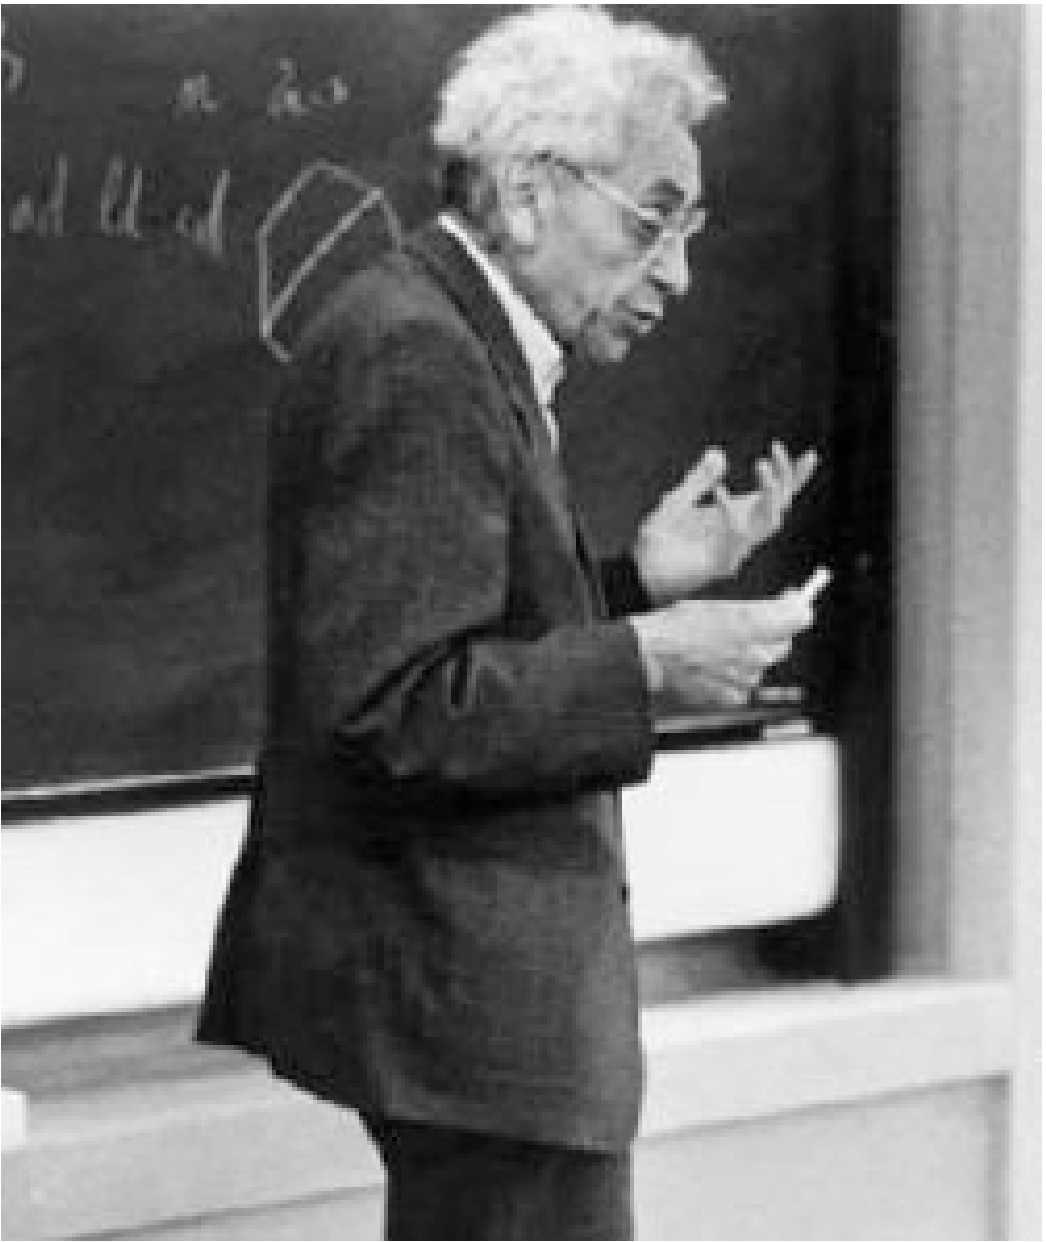
\includegraphics[scale=0.4]{Paul_Erdos} }
\end{frame}

\begin{frame}[fragile]\frametitle{Mathematics of counting and Kevin Bacon}

Combinatorics -- http://en.wikipedia.org/wiki/Combinatorics. 

\vspace{.3in}

What does Paul Erd\"{o}s have to do with Kevin Bacon ?

\end{frame}


\begin{frame}[fragile]\frametitle{Sample space}

\begin{defn}
A sample space $\cal S$ is the set of all possible outcomes
of an experiment.  \\
\end{defn}

\vspace{.1in}

Examples:

\begin{enumerate}

\item Experiment is flipping one coin -- Sample space is $\{H,T\}$. 

\item Experiment is flipping two coins -- Sample space is
  $\{HH,TT,HT,TH\}$. 

\item Experiment is flipping $n$ coins -- How many elements in the
  sample space ? 

\end{enumerate}
\end{frame}

\begin{frame}[fragile]\frametitle{Sample space}

\begin{defn}
A sample space $\cal S$ is the set of all possible outcomes
of an experiment.  
\end{defn}

\vspace{.1in}

Examples:

\begin{enumerate}
\setcounter{enumi}{4}
\item Experiment is playing five rounds of Russian roulette  -- Sample
  space is $\{D,LD,LLD,LLLD,LLLD\}$. Why is this different than coin 
flipping. 

\item Experiment is sequencing three nucleotides -- Sample space is 
$\{AAA,CCC,GGG,TTT,AAC,AAT,AAG,...,\}$. How big is this sample space ?
(Hint: There are four nucleotides.)


\end{enumerate}

\end{frame}


\begin{frame}[fragile]\frametitle{An event}

\begin{defn}
A event is any collection of outcomes contained in the sample space,
$\cal S$.
\end{defn}


Examples:

\begin{enumerate}

\item Flipping one coin -- Getting heads. 

\item Flipping two coins -- Getting two heads. 

\item Playing Russian roulette  -- Getting shot on the fourth spin. 

\item Sequencing nucleotides -- Your genome.

\end{enumerate}
\end{frame}

%%%%%%%%%%%%%%%%%%%%%%%%%%%%%%%%%%%%%%%%%%%%%%%%%%%%%%%%%%%%%%%%%%%%%%%%%%%%%%%%%%
\begin{frame}[fragile]\frametitle{}
\begin{center}
{\Large Set theory}

\end{center}
\end{frame}


\begin{frame}[fragile]\frametitle{Set theory}


An event is a set. \vspace{.1in}

\begin{defn}

\begin{enumerate}
\item The {\bf union} of two events $A$ and $B$  denoted $A \bigcup B$ 
  consists of outcomes that are either in $A$ or $B$.

\item The {\bf intersection} of two events $A$ and $B$ denoted $A \bigcap
  B$ consists of outcomes that both in $A$ and $B$.

\item The {\bf complement} of an event $A$ denoted $A'$ 
is the set of all outcomes in $\cal S$ not contained in $A$,
$A' = {\cal S} \backslash A$.
\end{enumerate}

\end{defn} 

\end{frame}

\begin{frame}[fragile]\frametitle{More set theory}

\begin{defn}
Two events $A$ and $B$ are {\bf mutually exclusive} or {\bf disjoint}
if  they have no outcomes in common, i.e. $A\cap B=\O$.
\end{defn} 

\vspace{.1in}

Being a Duke fan and a Carolina fan is mutually exclusive.\\
What is the event and what is the experiment ?
 
\end{frame}


%%%%%%%%%%%%%%%%%%%%%%%%%%%%%%%%%%%%%%%%%%%%%%%%%%%%%%%%%%%%%%%%%%%%%%%%%%%%%%%%%%
\begin{frame}[fragile]\frametitle{}
\begin{center}
{\Large Axioms}

\end{center}
\end{frame}





\begin{frame}[fragile]\frametitle{Axioms of probability}

Andrey Nikolaevich Kolmogorov -- measure theory.



\center{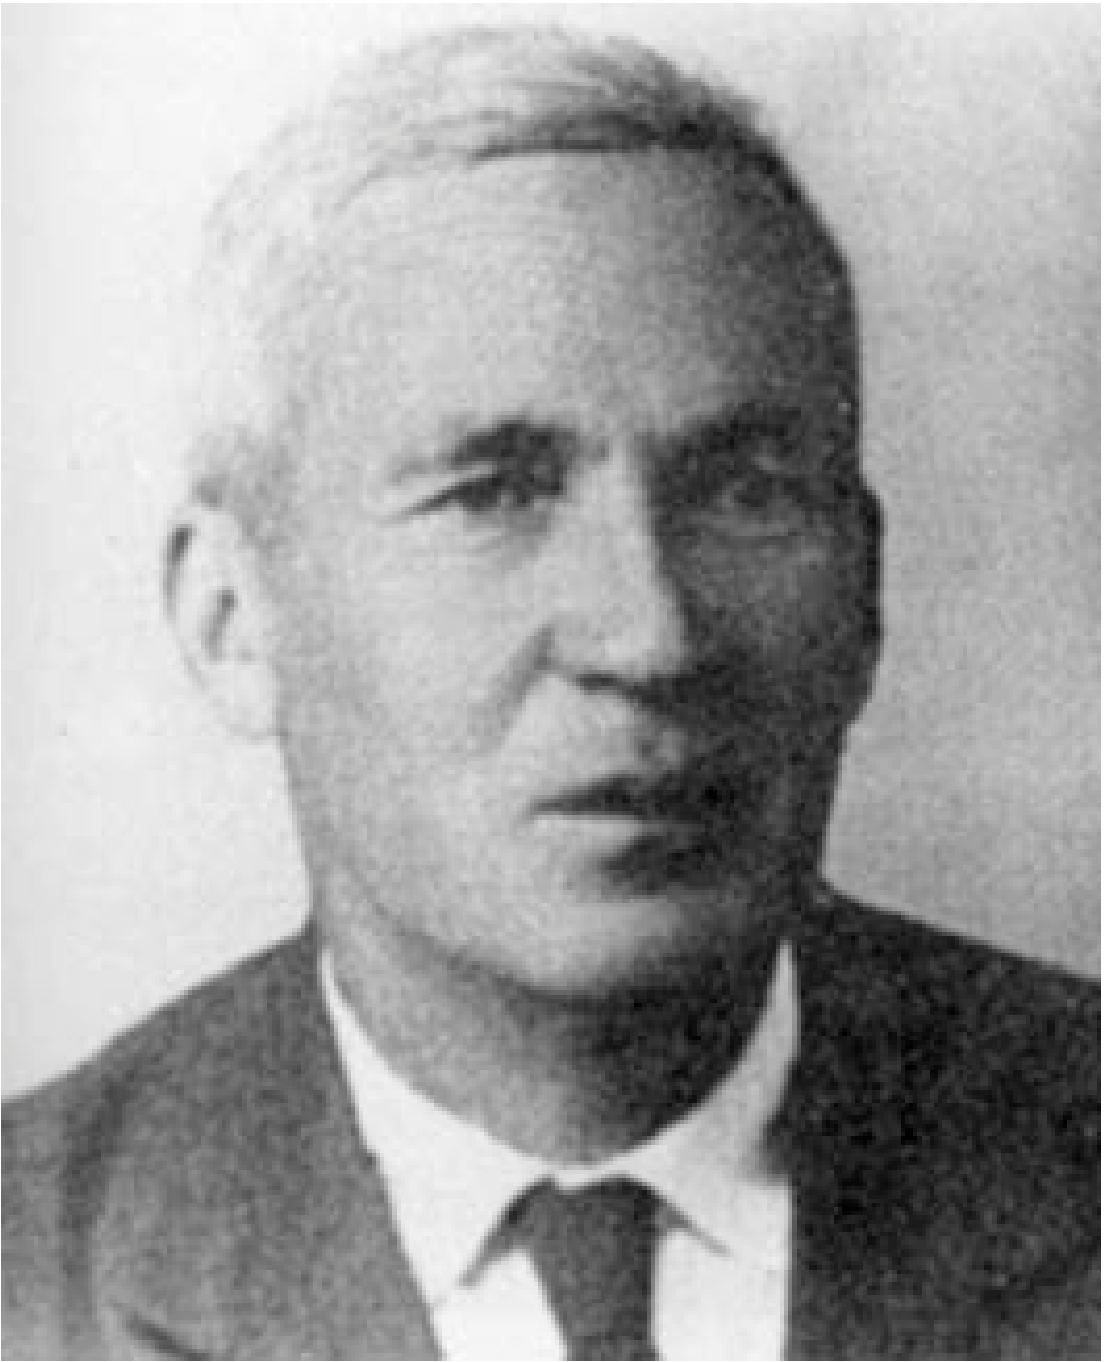
\includegraphics[scale=0.4]{Kolmogorov_7} }

\end{frame}


\begin{frame}[fragile]\frametitle{Axioms of probability}

Bruno de Finetti -- Dutch book.


\center{
\includegraphics[scale=0.3]{BrunodeFinetti} }

\end{frame}
 

\begin{frame}[fragile]\frametitle{Axioms of probability}


Given an experiment and a sample space $\cal S$, the objective of probability is to assign to each event $A$ a number $\pr(A)$, called the probability of the event $A$, which will give a precise measure of the chance that $A$ will occur. \\ 

\begin{enumerate}

\item Event: $A = \mbox{I fail every one in this class}$.  What is $\pr(A)$ ? 

\item Event: $A = \mbox{someone here wins the lottery}$.  What is $\pr(A)$ ? 

\item Event: $A = \mbox{I spin a quarter and it comes up heads}$.
   What  is $\pr(A)$ ?

\end{enumerate}

\end{frame}

\begin{frame}[fragile]\frametitle{Axioms of probability}

\begin{defn}

Axiom 1: For any event $A$, $\pr(A) \geq 0$ . 

Axiom 2: $\pr({\cal S}) =1$. 

Axiom 3: If $A_1,A_2,...,A_k$ are mutually exclusive events, then
$$\pr\left(A_1 \bigcup A_2 \bigcup \cdots \bigcup A_k\right) = \sum_{i=1}^k
\pr(A_i).$$ 
Let $k \rightarrow \infty$,  $A_1,A_2,A_3,...$ are mutually exclusive events
$$\pr\left(A_1 \bigcup A_2 \bigcup \cdots\right) = \sum_{i=1}^\infty \pr(A_i).$$

\end{defn}

\end{frame}


\begin{frame}[fragile]\frametitle{Axioms of probability}

Example: coin flip

${\cal S} = \{H,T\}$ and $H \bigcup T = {\cal S}$ 
\begin{eqnarray*}
1 & =& \pr({\cal S})\\ 
1 & = & \pr(H) + \pr(T) = \pr({\cal S}) \\ 
\pr(T) &= & 1 - \pr(H) = p 
\end{eqnarray*}

\end{frame}


\begin{frame}[fragile]\frametitle{Axioms of probability}

Example: Five rounds of Russian roulette on a six-bullet revolver.

$A_1 = \{D\}$, $A_2 = \{LD\}$, $A_3 = \{LLD\}$, $A_4 = \{LLLD\}$, $A_{5} = \{LLLLD\}$ \\ 
and $\pr(A_1)=...=\pr(A_{5}) = 1/6$, ${\cal S} = A_1 \bigcup A_2 \bigcup A_3 \bigcup \cdots$
so

\begin{eqnarray*}
1 & = & \pr({\cal S}) = \pr(A_1) + ... + \pr(A_5) 
\end{eqnarray*}

Missing something?

\end{frame}

%%%%%%%%%%%%%%%%%%%%%%%%%%%%%%%%%%%%%%%%%%%%%%%%%%%%%%%%%%%%%%%%%%%%%%%%%%%%%%%%%%
\begin{frame}[fragile]\frametitle{}
\begin{center}
{\Large Properties}

\end{center}
\end{frame}




\begin{frame}[fragile]\frametitle{Properties of probability -- Venn diagrams}

\begin{prop}
For any event $A$, $\pr(A) = 1- \pr(A')$ 
\end{prop} 

\vspace{.1in}

Sometimes $A'$ is easier to compute than $A$. \\ 
Example: Flip $n$ coins with $\pr(H) = p$. What is the 
probability of the event one or more heads ?
\begin{eqnarray*}
\pr(\bar{A}) &= &\pr(TTTTT\cdots) = (1-p)^n \\
\pr(A) &= & 1- (1-p)^n.
\end{eqnarray*}
\end{frame}

\begin{frame}[fragile]\frametitle{Properties of probability -- Venn diagrams}


\begin{prop}
If $A$ and $B$ are mutually exclusive, then 
$\pr\left(A \bigcap B\right) = 0$ and $A \bigcap B = \emptyset$. 
\end{prop}

\end{frame}


\begin{frame}[fragile]\frametitle{Properties of probability -- Venn diagrams}


\begin{prop}
For any two events $A$ and $B$, 
$$\pr\left(A \bigcup B\right) = \pr(A) +\pr(B) - \pr\left(A \bigcap B\right).$$
\end{prop}

\end{frame}


\begin{frame}[fragile]\frametitle{Properties of probability -- Venn diagrams}

For any three events $A$, $B$, $C$,
\begin{eqnarray*}
\pr \left(A \bigcup B  \bigcup C \right) &= &\pr(A) +\pr(B)+ \pr(C)\\
& & - \pr \left(A \bigcap B\right)- \pr\left(A \bigcap C \right) - \pr\left(B
  \bigcap C \right)\\
& & + \pr\left(A \bigcap B \bigcap C \right).
\end{eqnarray*}

\end{frame}

\begin{frame}[fragile]\frametitle{Properties of probability -- Venn diagrams}

For any three events $A$, $B$, $C$,
\begin{eqnarray*}
\pr \left(A \bigcup B  \bigcup C \right) &= &\pr(A) +\pr(B)+ \pr(C)\\
& & - \pr \left(A \bigcap B\right)- \pr\left(A \bigcap C \right) - \pr\left(B
  \bigcap C \right)\\
& & + \pr\left(A \bigcap B \bigcap C \right).
\end{eqnarray*}
\end{frame}

\begin{frame}[fragile]\frametitle{Properties of probability -- Venn diagrams}

In an experiment with $N$ outcomes that are equally likely the 
probability of any outcome $A$ is 
$$\pr(A) = p = \frac{1}{N}.$$  

\vspace{.2in}

Roll a six sided dice. What is $p$ ?
\end{frame}

%%%%%%%%%%%%%%%%%%%%%%%%%%%%%%%%%%%%%%%%%%%%%%%%%%%%%%%%%%%%%%%%%%%%%%%%%%%%%%%%%%
\begin{frame}[fragile]\frametitle{}
\begin{center}
{\Large Combinatorics -- counting}

\end{center}
\end{frame}



\begin{frame}[fragile]\frametitle{Counting 101}

When you have to count go through the following checklist 

\begin{enumerate}

\item Does order matter ? 

\item Can objects be chosen only once ? 

\item Can I break the problem into simpler computations ? 

\item Is the complement simpler to work with ? 
 
\item Can I simplify computations by conditioning ? 

\end{enumerate}

\end{frame}

\begin{frame}[fragile]\frametitle{Order matters with repetition}

Given a set of objects for example $A,B,C,D$. \\
 

Assume
\begin{enumerate}

\item Order matters: $ABC$ is different from $CBA$.

\item Objects can be selected more than once, i.e. $AAA$ is possible.

\end{enumerate}

\end{frame}


\begin{frame}[fragile]\frametitle{Order matters with repetition}


An ordered collection of $k$ objects is a $k$-tuple. \\ 

\vspace{.1in}

Your genome is a $k$-tuple, $\{AAACTGATTTCCC \cdots \}$,
with $k \approx 3$ billion. \\ 

\vspace{.1in}

A fixed price meal is a $k$-tuple, $\{\mbox{app},\mbox{main},\mbox{dessert}\}$,
with $k = 3$. 

\end{frame}




\begin{frame}[fragile]\frametitle{Order matters - product rule}

\begin{prop}
A set consists of ordered collections of $k$-tuples with $n_1$ choices
for element $1$, $n_2$ choices for element $2$ ,..., and $n_k$ choices
for element $k$. The number of possible $k$-tuples are 
$n_1 n_2 \cdots n_k$.
\end{prop}
 
\end{frame}


\begin{frame}[fragile]\frametitle{Fixed price menu}

\center{
\includegraphics[scale=0.4]{ref} }

\end{frame}


\begin{frame}[fragile]\frametitle{Fixed price menu}

Appetizers: $n_1 = 6$ \\
Mains: $n_2 = 6$ \\
Desserts $n_3 = 6$ \\

Number of meals: $n_1 \times n_2 \times n_3 = 216$.
\end{frame}

\begin{frame}[fragile]\frametitle{An argument for intelligent design}


Your genome is a $k$-tuple, with $k \approx 3$ billion. \\ 

William A. Dembski makes the following argument.
\begin{enumerate}
\item Assume that $A,C,T,G$ are equally likely. 
\item Assume that order matters and an amino acid in one position
does not effect others. 
\item The probability of your genome is $1/4^{30,000,000,000}$. 
\item Astronomically small chance so cannot be random, or evolve from
random mutations.
\end{enumerate}

\end{frame}

\begin{frame}[fragile]\frametitle{Order matters without repetition - permutation}

Given a set of objects for example $A,B,C,D$. \\
 
Assume
\begin{enumerate}

\item Order matters: $ABC$ is different from $CBA$.

\item Objects cannot be selected more than once: $AAA$ is not possible,
neither is $AAB$. $ACB$ is possible.

\end{enumerate}

\end{frame}

\begin{frame}[fragile]\frametitle{Order matters without repetition - permutation}

Example: Pick a starting lineup for Duke given 
the $12$ people on the roster. \\


$$P_{5,12} = 12  \times 11  \times 10  \times 9
 \times 8.$$ 
  
More generally
$$P_{k,n} = \frac{n!}{(n-k)!},$$
where $n! = n(n-1)(n-2)(n-3)\cdots 1$ and $0! = 1$. \\

\end{frame}

\begin{frame}[fragile]\frametitle{Order doesn't matter without repetition -
    combinations}

Given a set of objects for example $A,B,C,D$. \\
 
Assume
\begin{enumerate}

\item Order does not matter: $ABC$ is the same as $CBA$.

\item Objects cannot be selected more than once: $AAA$ is not possible,
neither is $AAB$. $ACB$ is possible.

\end{enumerate}
\end{frame}


\begin{frame}[fragile]\frametitle{Order doesn't matter without repetition - combinations}

\begin{defn}
Given $n$ distinct objects, any unordered subset of size 
$k$ objects is a combination. The number of combinations
is $\binom{n}{k}$ or $n$ choose $k$. 
\end{defn}
\vspace{.1in}

A bridge hand is a combination. \\ 

\vspace{.1in}

So is a poker hand.
\end{frame}


\begin{frame}[fragile]\frametitle{Order doesn't matter without repetition - combinations}

An example: Given the set $\{A,B,C,D,E\}$ how many combinations of
size three ?  

\vspace{.1in}

\begin{enumerate}

\item First observation: $P_{3,5} > \binom{5}{3}$, why ? \\ 
Permutations $\{ABC\},\{ACB\},\{BCA\},\{BAC\},\{CBA\},\{CAB\}$\\ 
Combination $\{ABC\}$.   

\item Second observation: for any combination of size $3$ there are 
$3!=6$ permutations.  

\end{enumerate}
\end{frame}


\begin{frame}[fragile]\frametitle{Order doesn't matter without repetition - combinations}

An example: Given the set $\{A,B,C,D,E\}$ how many combinations of
size three ?  

\vspace{.1in}

\begin{enumerate}
\setcounter{enumi}{2}

\item Third observation: 
\begin{eqnarray*}
P_{3,5}& = & \binom{5}{3} \times 3! \\
\binom{5}{3} &=&\frac{P_{3,5}}{3!}=  \frac{5!}{3!(5-3)!}. 
\end{eqnarray*}

\item Induction:  
$$\binom{n}{k} = \frac{n!}{k!(n-k)!}.$$

\end{enumerate}
\end{frame}

\begin{frame}[fragile]\frametitle{Poker hands}

$52$ playing cards and you are dealt $5$ cards (a hand). \\ 
$4 \mbox{ suits }: \clubsuit, \heartsuit, \spadesuit,
\diamondsuit$. \\ 
Each suit has $13$ cards $2-9,J,Q,K,A$. \\ 
You want the best hand. \\
\center{Some poker hands \\
None the same \\
Pair \\
Two pairs \\
Three of a kind \\
Full house \\
Four of a kind \\
Royal flush\\}
\end{frame}


\begin{frame}[fragile]\frametitle{Poker hands}


Number of total poker hands:
$$\binom{52}{5} = 2,598,960.$$ 
\end{frame}


\begin{frame}[fragile]\frametitle{None the same}

Number of none the same: \\ 

Counting strategy 1: break into cases and then multiply \\
Cases: face cards and suits. \\ 
Choices of faces $\binom{13}{5}$: $5$ different faces out of $13$ for
example $\{3 \,8 \, 5 \, 2 \, 9\}$. \\ 
Choices of suits $4 \times 4 \times 4 \times 4 \times 4$: each card
can be one of four suits  for example $\{\clubsuit \heartsuit \spadesuit
\diamondsuit \heartsuit\}$\\ 
Total: $\binom{13}{5}\times 4^5 = 1,317,888$ \\ 
$$\pr(\mbox{none the same}) = \frac{1,317,888}{2,598,960} = 50.7\%.$$

\end{frame}


\begin{frame}[fragile]\frametitle{Flush}

Choices of faces $\binom{13}{5}$: $5$ different faces out of $13$. \\
Choices of suits $4$. \\
Total: $\binom{13}{5}\times 4 = 5148$ \\ 
$$\pr(\mbox{flush}) = \frac{5148}{2,598,960} = 0.2\%.$$

\end{frame}



\begin{frame}[fragile]\frametitle{None the same no flush}

This example uses the idea that sometimes the complement
is easier to count. \\ 
The set $\{\mbox{None the same no flush}\}$ can be written
as
$$\{\mbox{None the same no flush}\} = \{\mbox{None the same}\} - 
\{\mbox{None the same flush}\}.$$ 
Observe: $\{\mbox{None the same flush}\}=\{\mbox{flush}\}$. \\ 
Total: $\binom{13}{5}\times 4^5 - \binom{13}{5}\times 4 = 1,312,740$ \\ 
$$\pr(\mbox{none the same no flush}) = \frac{5148}{2,598,960} = 50.5\%.$$

\end{frame}


%%%%%%%%%%%%%%%%%%%%%%%%%%%%%%%%%%%%%%%%%%%%%%%%%%%%%%%%%%%%%%%%%%%%%%%%%%%%%%%%%%
\begin{frame}[fragile]\frametitle{}
\begin{center}
{\Large Conditional probability}

\end{center}
\end{frame}


\begin{frame}[fragile]\frametitle{Conditional probability}

The notation $\pr(A|B)$ denotes the probability of $A$ given $B$
occurred. \\ 

An example of this: $A$ denotes a baboon testing positive 
for Syphilis, $B$ denotes the baboon has Syphilis. \\ 
$$\pr(A|B) > \pr(A).$$ 

\vspace{.2in}
How do baboons get Syphilis ?
\end{frame}

\begin{frame}[fragile]\frametitle{Conditional probability}

\begin{defn}

Given two events $A$ and $B$ with $\pr(B) > 0$, the
{\bf conditional probability} of $A$ given $B$ has
occurred is defined as
$$\pr(A|B) = \frac{\pr(A \bigcap B)}{\pr(B)}.$$
\end{defn}

\end{frame}

\begin{frame}[fragile]\frametitle{Conditional probability}
Some examples:


\small{

\begin{table}[htb]
\centerline{
\begin{tabular}{|l|l|l|}
\hline
& Has disease & Doesn't have disease\\
\hline
Test is positive & $9/1000$ & $50/1000$ \\
\hline
Test is negative & $1/1000$ & $940/1000$ \\
\hline
\end{tabular}
} 

\end{table}
}

Two questions: \\
$\pr(\mbox{have disease}|\mbox{test is positive})$ and 
$\pr(\mbox{test is positive}|\mbox{have disease})$.
\end{frame}


\begin{frame}[fragile]\frametitle{Conditional probability}

The events $A = \{\mbox{have disease}\}$ and $B = \{\mbox{test
  positive}\}$. \\ 
$\pr(A,B) = 9/1000 = .9\%$ and $\pr(A) = 9/1000+1/1000 = 1\%$ and 
$\pr(B) = 9/1000+50/1000 = 5.9\%$ \\ 
\begin{eqnarray*}
\pr(A|B) & = & \frac{\pr(A \bigcap B)}{\pr(B)} = \frac{.009}{.059}= 15\% \\
\pr(B|A) & = & \frac{\pr(A \bigcap B)}{\pr(A)} = \frac{.009}{.01} =
90\%.
\end{eqnarray*} 

$\pr(\mbox{have disease}|\mbox{test is positive}) = 15\%$ \\
$\pr(\mbox{test is positive}|\mbox{have disease}) = 90\%$.

\end{frame}


\begin{frame}[fragile]\frametitle{Conditional probability}

\begin{prop}[Multiplication rule]
$$\pr(B \bigcap A) = \pr(B |A) \times \pr(A).$$
\end{prop} 


\begin{prop}[Law of total probability]
Let $A_1,...,A_k$ be mutually exclusive and exhaustive events. Then
for any other event $B$
$$\pr(B) = \sum_{i=1}^k \pr(B |A_i) \times \pr(A_i).$$
\end{prop}

\end{frame}

\begin{frame}[fragile]\frametitle{Conditional probability}

Proof of Law of total probability \\ 

By logic \\
$$B = \mbox{($A_1$ and $B$) or ($A_2$ and $B$) or ... or ($A_k$ and  $B$)}.$$ 

In equation form
$$B = (A_1 \bigcap B) \bigcup (A_2 \bigcap B) \bigcup ... \bigcup (A_K
\bigcap B)).$$ 

This implies
$$\pr(B) = \pr \left[(A_1 \bigcap B) \bigcup (A_2 \bigcap B) \bigcup
    ... \bigcup (A_K \bigcap B)\right].$$ 

\end{frame}

\begin{frame}[fragile]\frametitle{Conditional probability}

Proof of Law of total probability \\ 

$$\pr(B) = \pr \left\{(A_1 \bigcap B) \bigcup (A_2 \bigcap B) \bigcup
    ... \bigcup (A_K \bigcap B)\right\}.$$ 
Since $A_i$ are exclusive and exhaustive
$$\pr(B) = \sum_{i=1}^k \pr(A_i \bigcap B) = \sum_{i=1}^k \pr(B |A_i)
\times \pr(A_i) .$$
The last step is by the multiplication rule.
\end{frame}

\begin{frame}[fragile]\frametitle{Bayes' theorem}

\begin{thm}
Let $A_1,...,A_k$ be mutually exclusive and exhaustive events with 
$\pr(A_i) > 0$ for all $i=1,...,k$. Then
for any other event $B$ with $\pr(B) > 0$
$$\pr(A_j|B) = \frac{\pr(A_j \bigcap B)}{\pr(B)} = \frac{\pr(B|A_j)
  \pr(A_j)}{\sum_{i=1}^k \pr(B|A_i) \pr(A_i)}, \, \, \, \, \, j=1,...,k.
$$
\end{thm}

\end{frame}


\begin{frame}[fragile]\frametitle{Bayes' theorem}

A common application of Bayes' theorem is the following:
$$\pr(\mbox{model}|\mbox{data}) = \frac{\pr(\mbox{data}|\mbox{model})
  \, \pr(\mbox{model})}{\pr(\mbox{data})}.$$ 
 
The important quantities are:
\begin{enumerate}
\item Likelihood: $\pr(\mbox{data}|\mbox{model})$ 
\item Prior: $\pr(\mbox{model})$ 
\item Posterior: $\pr(\mbox{model}|\mbox{data})$ 
\end{enumerate}
\end{frame}


\begin{frame}[fragile]\frametitle{The reverend Thomas Bayes}
\center{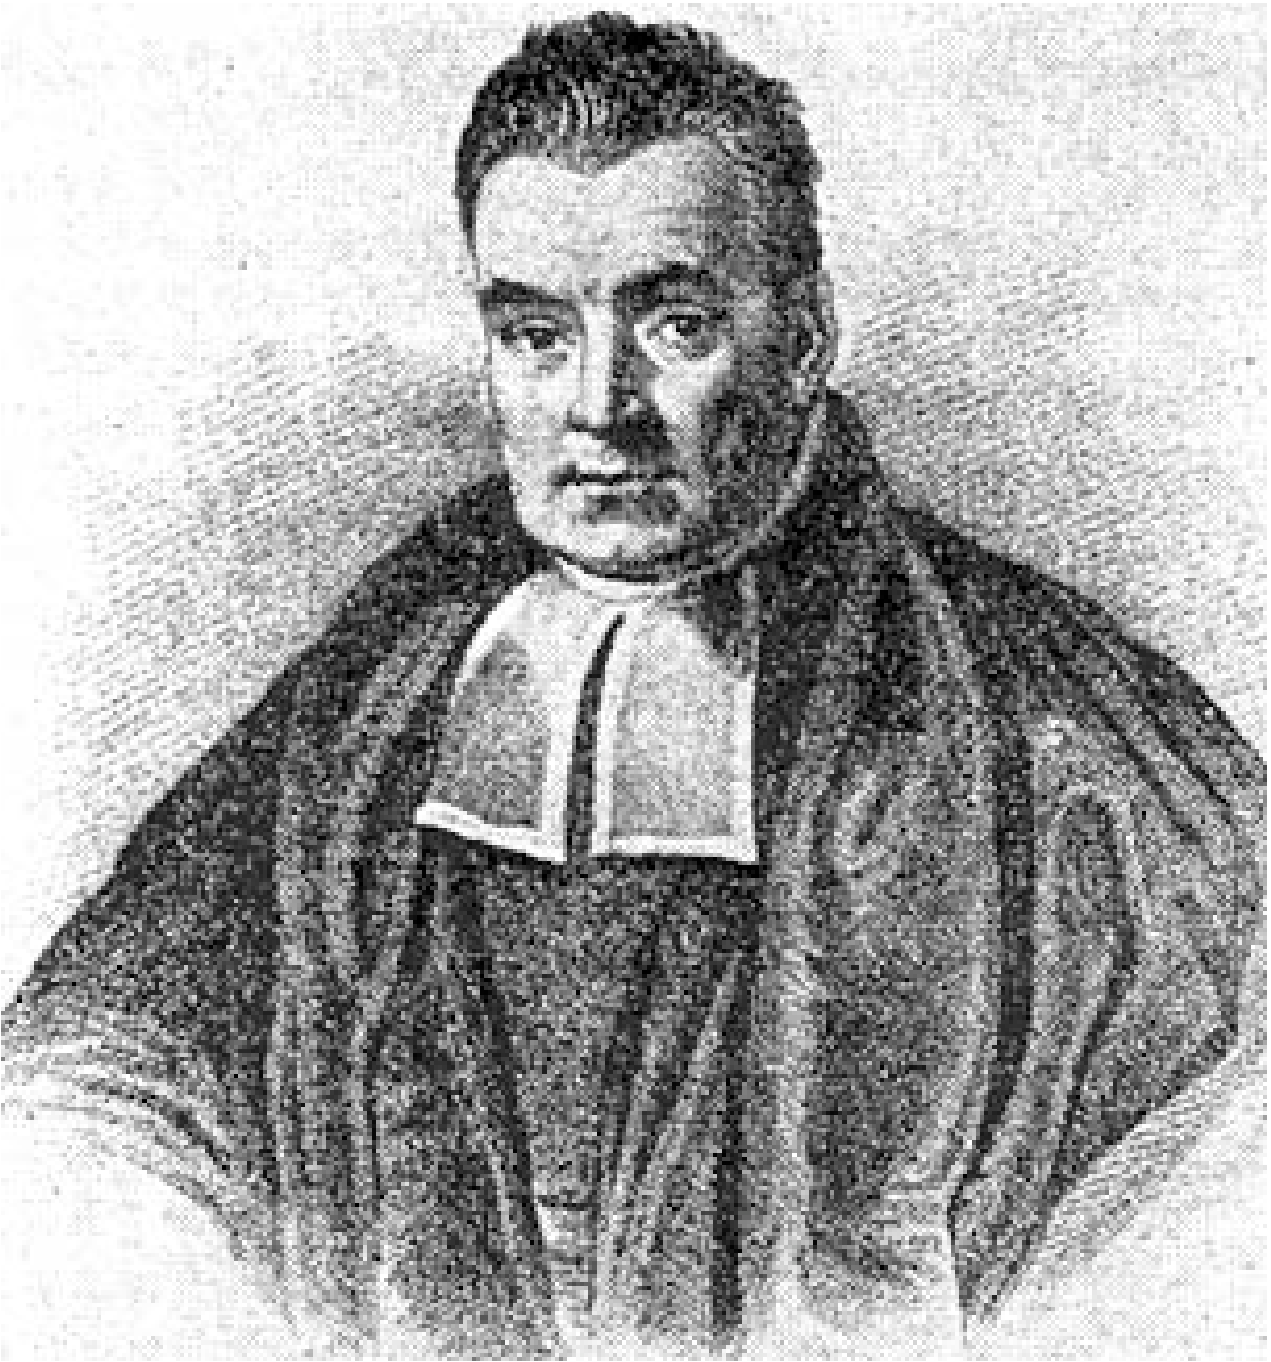
\includegraphics[scale=0.4]{Thomasbayes} }
\end{frame}

\begin{frame}[fragile]\frametitle{Monty Hall}
\alert{\url{http://math.ucsd.edu/~crypto/Monty/monty.html}}
\end{frame}


\begin{frame}[fragile]\frametitle{Monty Hall}


Should I switch or not ? \\ 

Say you pick door $A$ and Monty opens door $B$ \\ 

The prior probability that the prize is behind
door $\pr(A) = 1/3$. \\ 

Probability Monty opens door $B$ if the prize is behind $A$ is
$\pr(\mbox{Monty opens }B|A) = 1/2$. \\ 

Probability Monty opens door $B$ if the prize is behind $B$ is
$\pr(\mbox{Monty opens }B|B) = 0$. \\ 

Probability Monty opens door $B$ if the prize is behind $C$ is
$\pr(\mbox{Monty opens }B|C) = 1$. 

\end{frame}


\begin{frame}[fragile]\frametitle{Monty Hall}


Say you pick door $A$ and Monty opens door $B$ \\


The probability that Month opens door $B$ is 
\begin{eqnarray*}
\pr(B) &=& \pr(A) \times \pr(B|A) + \pr(B) \times \pr(B|B) + \pr(C)
\times \pr(B|C)\\
&  = & 1/6 + 0 + 1/3 = 1/2. 
\end{eqnarray*}

By Bayes rule
\begin{eqnarray*}
\pr(A|B) &=& \frac{\pr(A) \times \pr(B|A)}{\pr(B)}\\
         & = & (1/6)/(1/2) = 1/3 \\  
\pr(C|B) &=& \frac{\pr(C) \times \pr(B|C)}{\pr(B)}\\
         & = & (1/3)/(1/2) = 2/3. 
\end{eqnarray*}
\end{frame}

%%%%%%%%%%%%%%%%%%%%%%%%%%%%%%%%%%%%%%%%%%%%%%%%%%%%%%%%%%%%%%%%%%%%%%%%%%%%%%%%%%
\begin{frame}[fragile]\frametitle{}
\begin{center}
{\Large Independence}

\end{center}
\end{frame}




\begin{frame}[fragile]\frametitle{Independence}

\begin{defn}

Two events $A$ and $B$ are {\bf independent} if $\pr(A|B) = \pr(A)$ and
are {\bf dependent} otherwise.
\end{defn}

\end{frame}


\begin{frame}[fragile]\frametitle{Independence}

\begin{prop}
$A$ and $B$ are independent if and only if
$$\pr(A \bigcap B) = \pr(A) \times \pr(B).$$
\end{prop}

\end{frame}

\begin{frame}[fragile]\frametitle{Independence}

\begin{defn}
Events $A_1,...,A_n$ are {\bf mutually independent} if for every 
$k=2,3,...n$ and every subset of indices $i_1, \,i_2,...,i_k$
$$\pr(A_{i_1} \bigcap A_{i_2} \bigcap ... A_{i_k}) = \pr(A_{i_1})
\times \pr(A_{i_2}) \times ... \pr(A_{i_k}).$$
\end{defn}

\end{frame}


\begin{frame}[fragile]\frametitle{Independence}

Examples:

Events $A_1, A_2, A_3$ 
\begin{eqnarray*}
\pr(A_1 \bigcap A_2 \bigcap A_3) &= & \pr(A_1) \times \pr(A_2) \times
\pr(A_3) \\  
 &= & \pr(A_1 \bigcap A_2) \times \pr(A_3) \\ 
 &= & \pr(A_1 \bigcap A_3) \times \pr(A_2) \\ 
 &= & \pr(A_2 \bigcap A_3) \times \pr(A_1). 
\end{eqnarray*}
\end{frame}

\begin{frame}[fragile]\frametitle{Mathematical definition}

\begin{defn}
A random variable is a function that maps an event from the
sample space $\cal S$ to a real number:
$$X: \omega \rightarrow \rr,$$
where $\omega \in {\cal S}$.
\end{defn}

\end{frame}



\begin{frame}[fragile]\frametitle{Intuition}

Think of a function as a machine. It has inputs and outputs:
$f:x \rightarrow y$. 

A catapult
\center{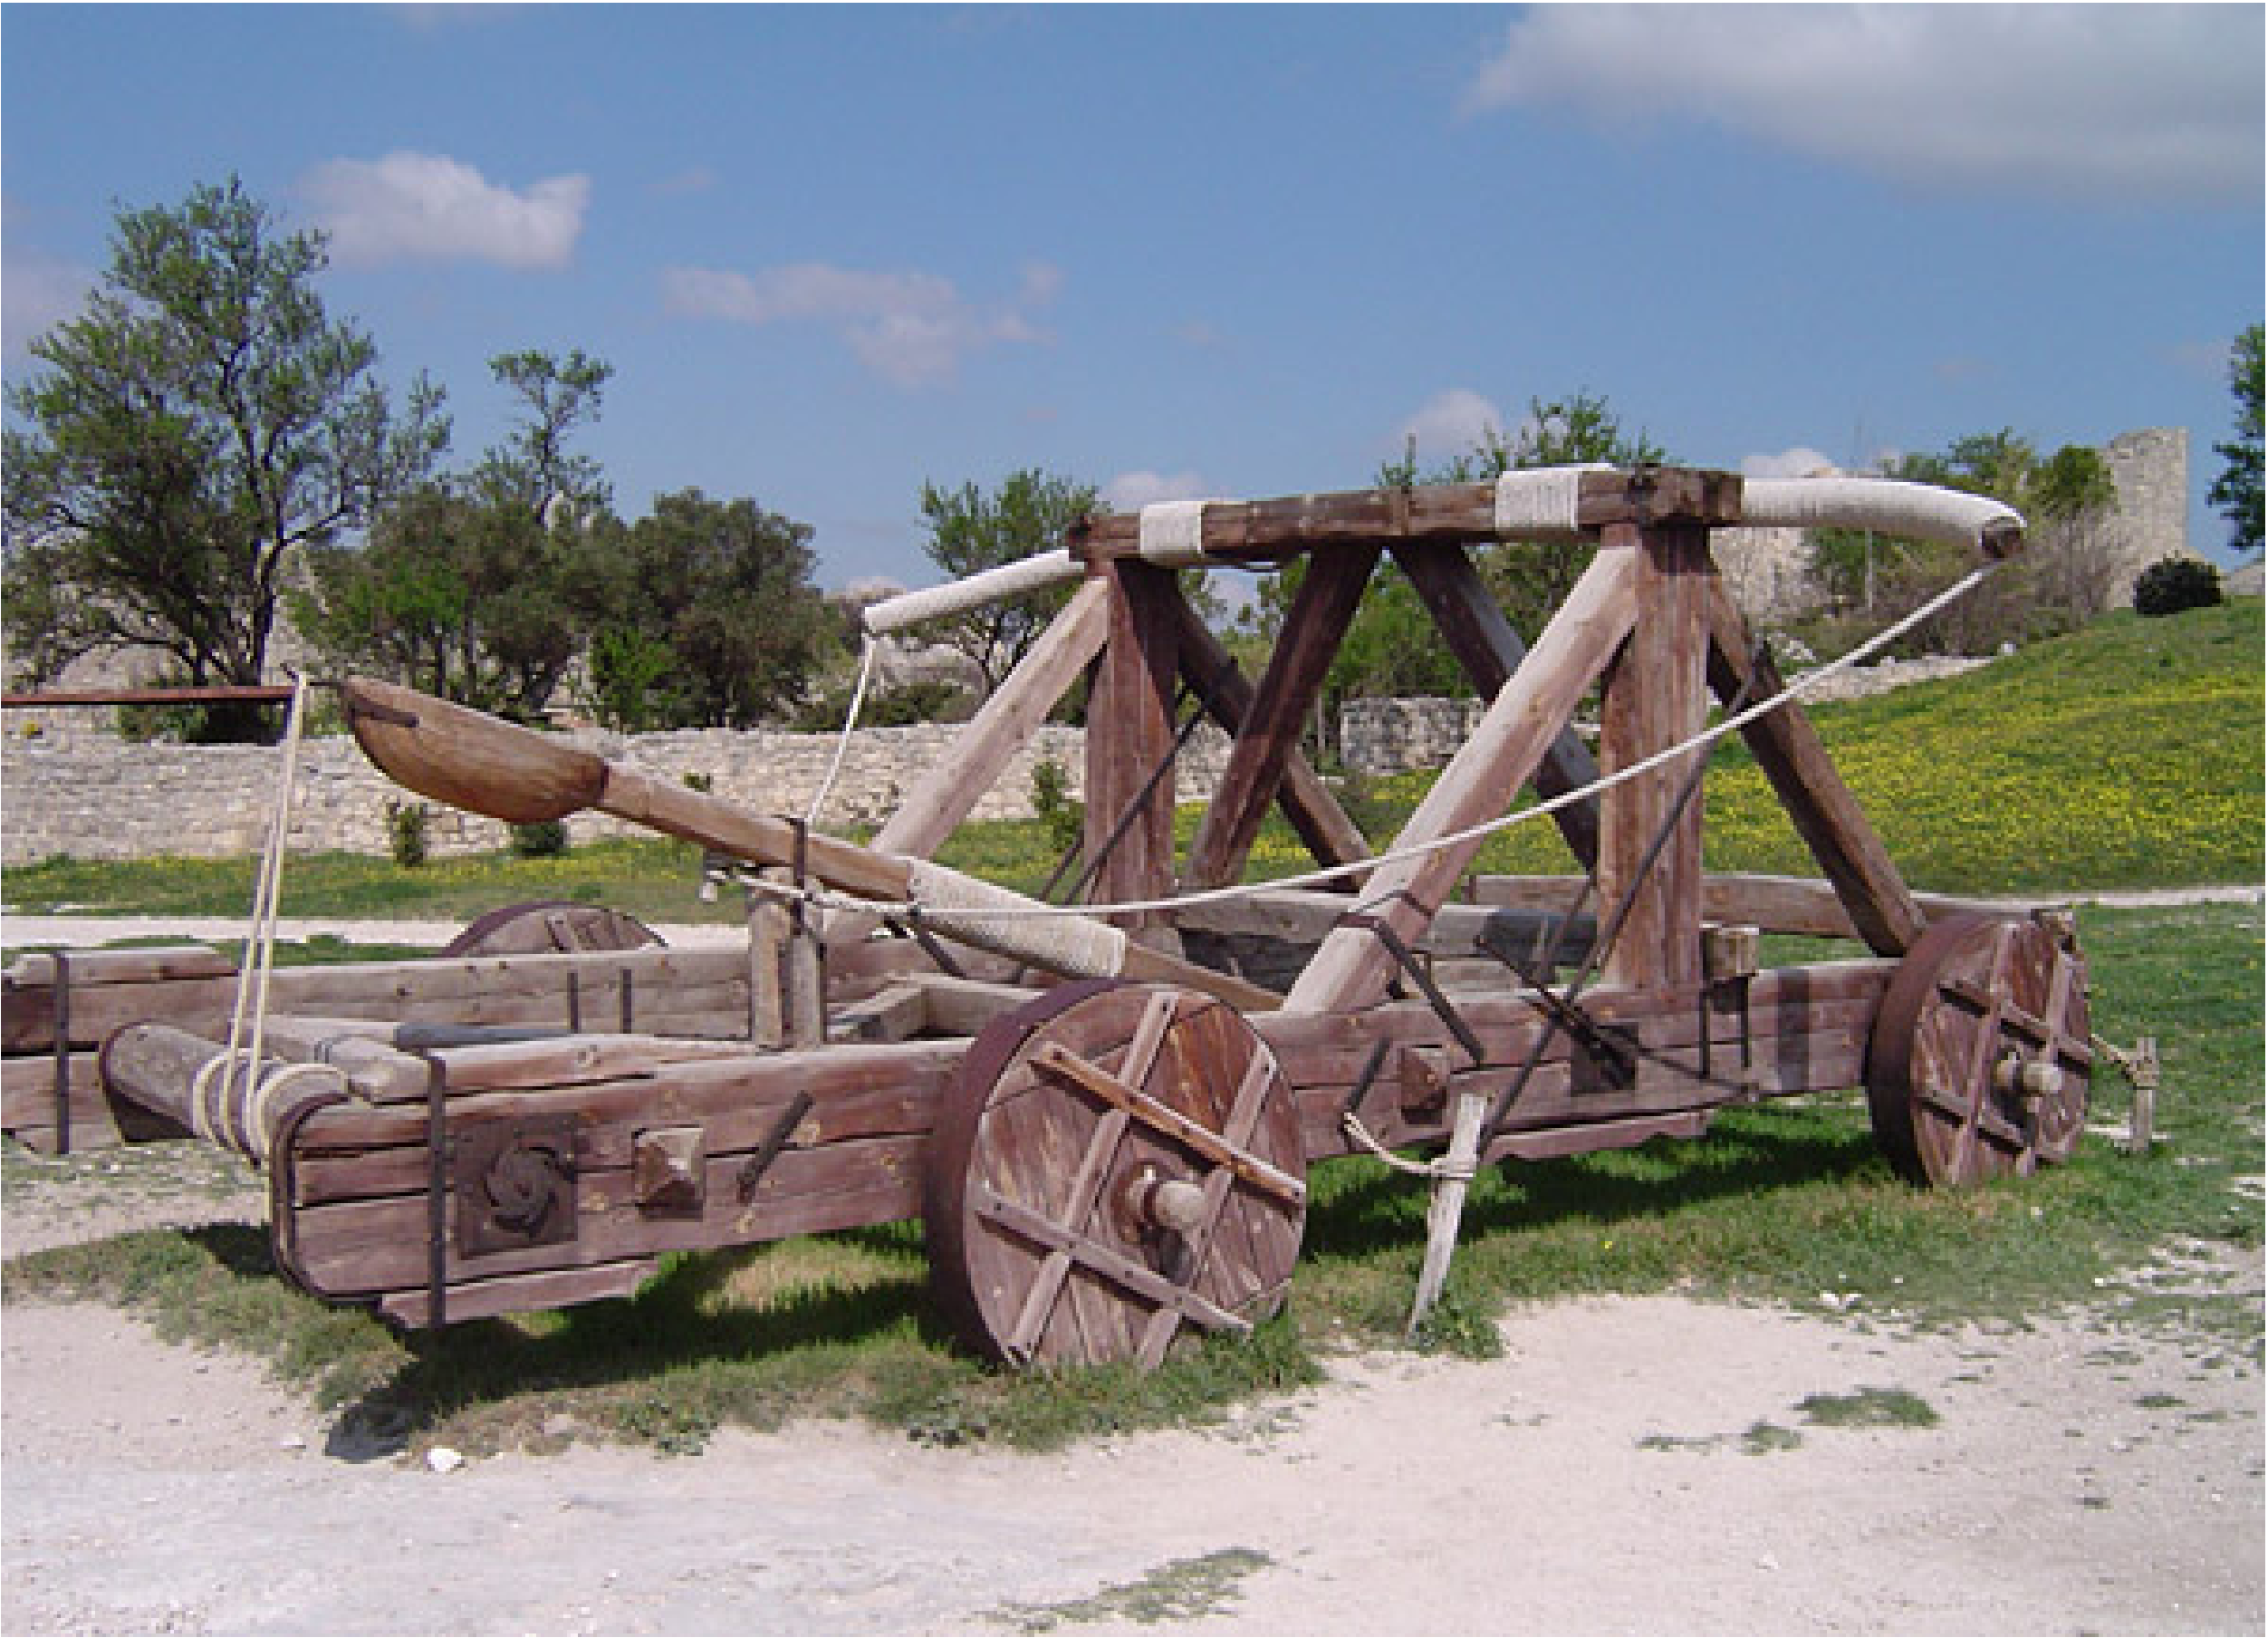
\includegraphics[scale=0.3]{Replica_catapult} }

\end{frame}


\begin{frame}[fragile]\frametitle{Intuition}

The catapult takes as inputs: a rock and tension cord. \\
The output is the distance the rock flies.

\end{frame}


\begin{frame}[fragile]\frametitle{Intuition}

The machine/function is now the flipping of a quarter by 
my thumb. The output is one of two possibilities: $\{H,T\}$.
Let us call $H=1$ and $T=0$. \\  

This function is a (discrete) random variable it maps $\{H,T\}$ into
real numbers $\{0,1\}$, \\ 
Why is this function random ? 
Why is it discrete ?


\end{frame}




\begin{frame}[fragile]\frametitle{Intuition}

Back to the catapult. Even if we know exactly the size and
shape of the rock as well as the tension of the cord,
the distance the rock flies may not always be the same
due to variation in wind and many other factors. \\ 

The catapult is a (continuous) random variable it maps 
the state of the catapult to real numbers $[0,\infty)$. \\ 
Why is this function random ? 
Why is it continuous ?


\end{frame}



\begin{frame}[fragile]\frametitle{Discrete versus continuous rv}

\begin{defn}
A {\bf discrete} random variable is a rv  which takes a finite or
countable number of values. \\
A {\bf continuous} random variable is a rv  which takes values in an
interval of the real line or all of the real line.
\end{defn}

\end{frame}


\begin{frame}[fragile]\frametitle{Bernoulli random variable}

\begin{defn}
A random variable that takes values $0$ or $1$ is called a {\bf
  Bernoulli random variable}.
\end{defn} 

\center{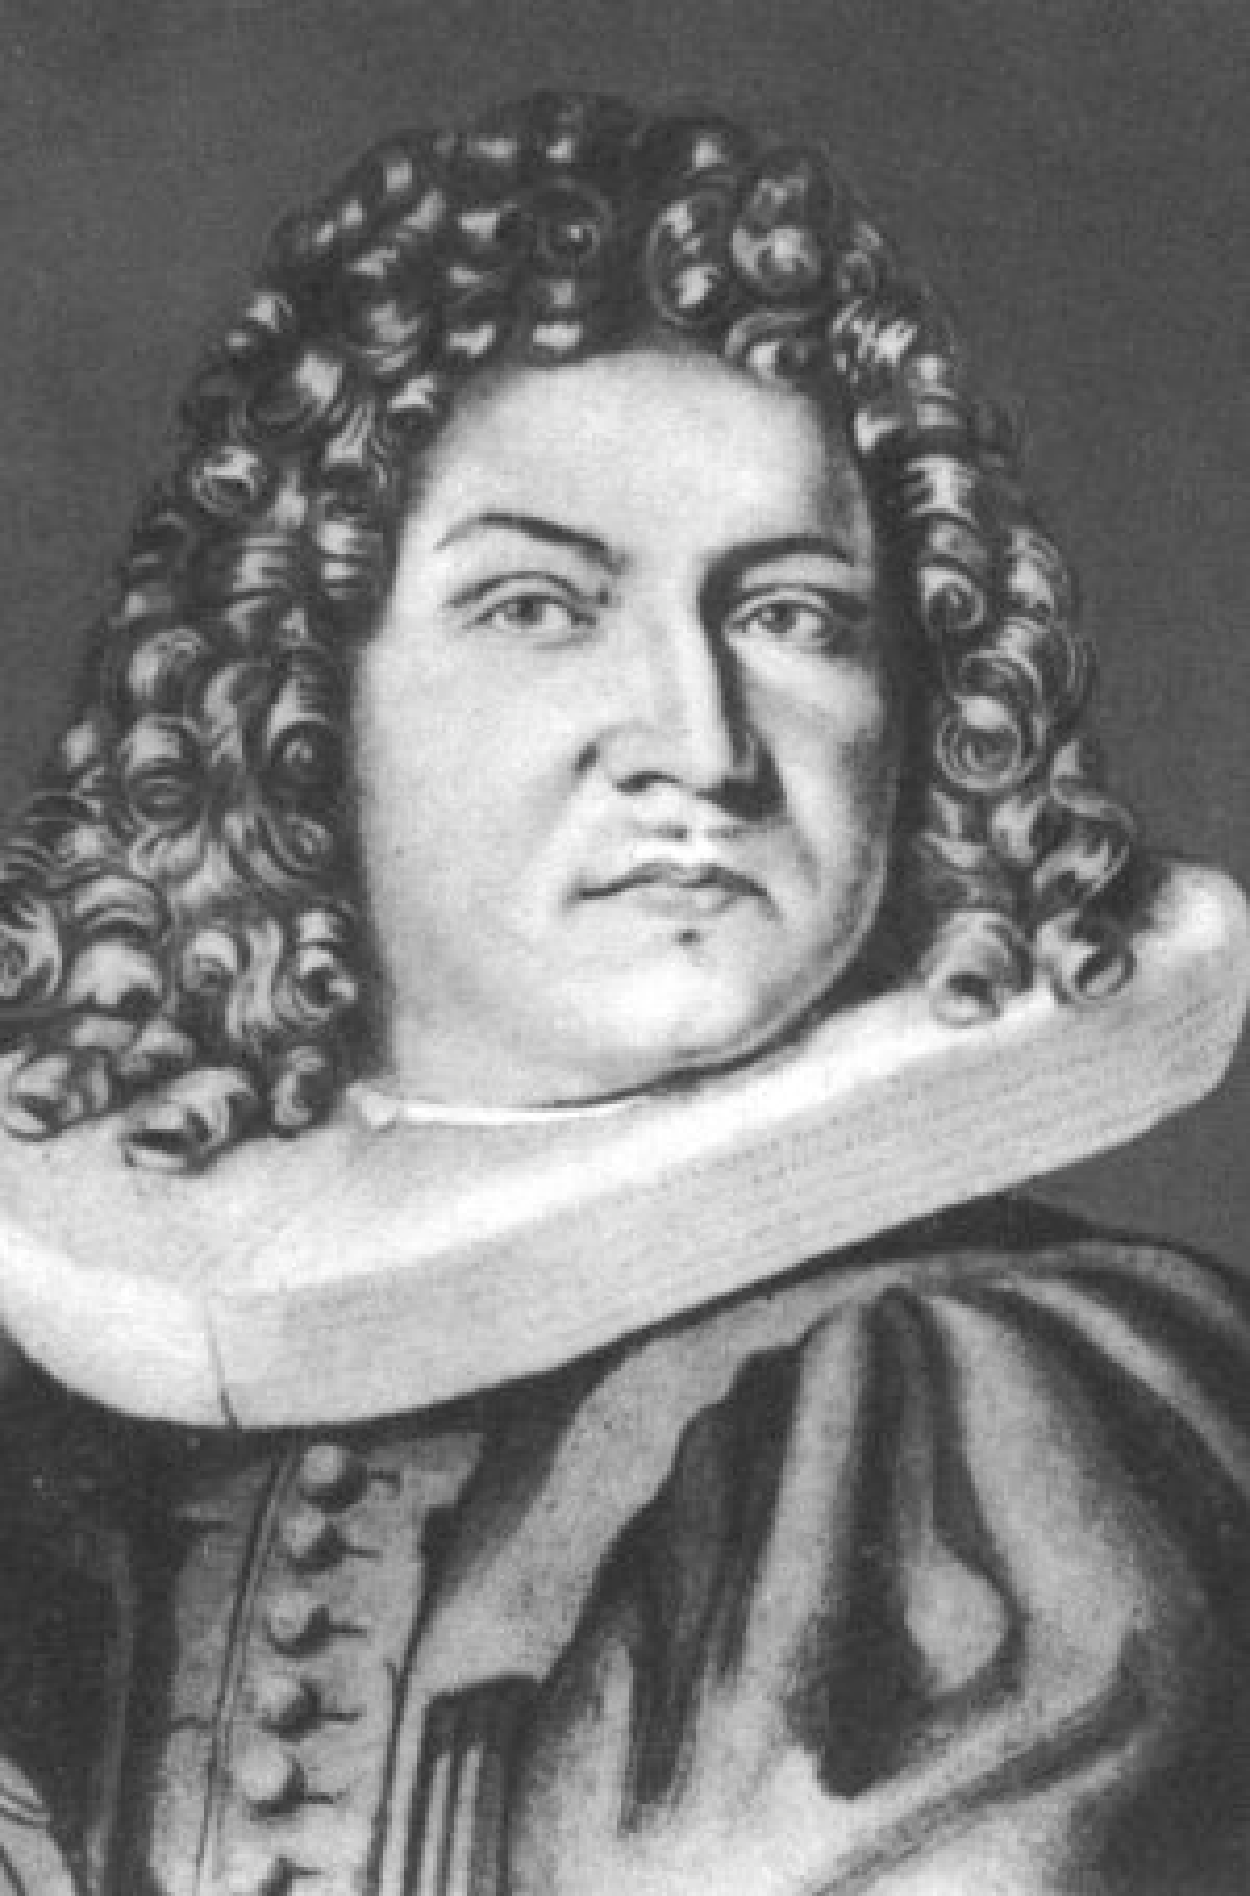
\includegraphics[scale=0.25]{Jakob_Bernoulli} }

\end{frame}


%%%%%%%%%%%%%%%%%%%%%%%%%%%%%%%%%%%%%%%%%%%%%%%%%%%%%%%%%%%%%%%%%%%%%%%%%%%%%%%%%%
\begin{frame}[fragile]\frametitle{}
\begin{center}
{\Large Distributions for discrete random variables}

\end{center}
\end{frame}



\begin{frame}[fragile]\frametitle{Distribution function}

\begin{defn}
The {\bf probability distribution function} or {\bf probability
mass function} of a discrete random variable is defined for
every possible $x$ by
$$p(x) = \pr(X=x) = \pr(X(s) = x: \mbox{for all } s \in {\cal S}).$$
\end{defn} 

\end{frame}


\begin{frame}[fragile]\frametitle{An example}

\center{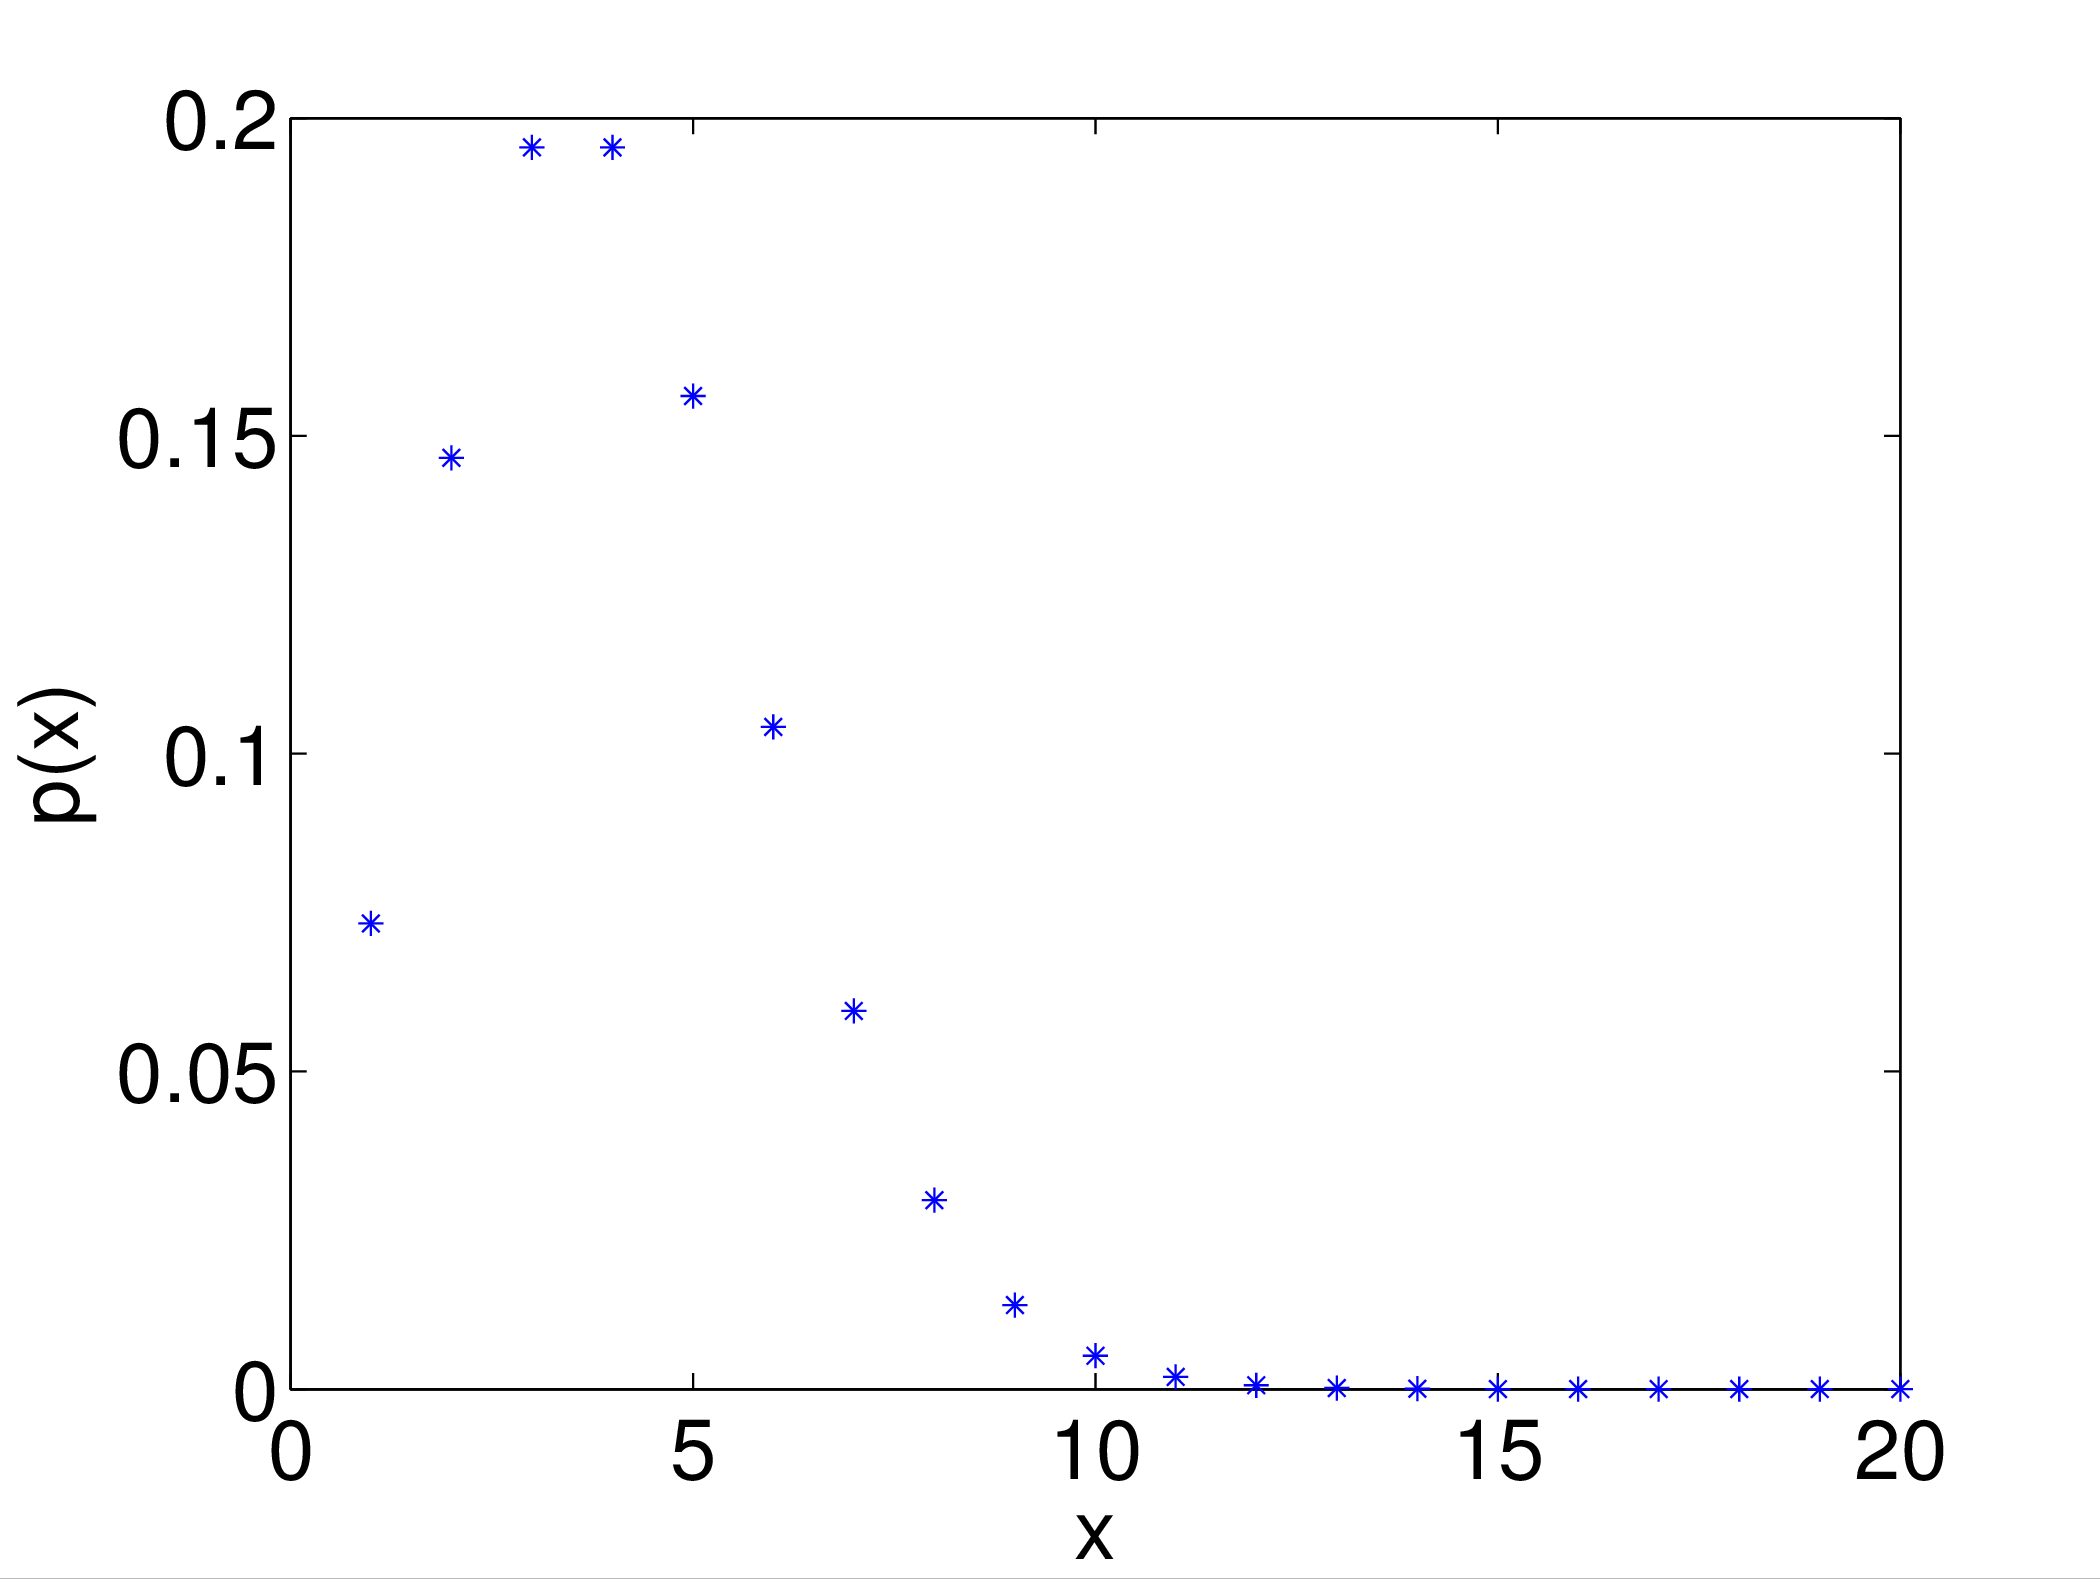
\includegraphics[scale=0.5]{poiss1} }

\end{frame}



\begin{frame}[fragile]\frametitle{Matlab code}



x= 1:20; \\
y = poisspdf(x,4); \\
plot(x,y,'*') \\

\end{frame}




\begin{frame}[fragile]\frametitle{Some properties}


\begin{enumerate}

\item $p(x) \geq 0$ for all $X=x$ 

\item $\sum_x p(x) =1$

\end{enumerate}

\end{frame}



\begin{frame}[fragile]\frametitle{Parameter of a pdf}

\begin{defn}
If $p(x)$ is parameterized by a quantity $\alpha$ then $\alpha$
is the parameter of the pdf and the set of pdfs characterized
by varying $\alpha$ is called a {\bf family} of distribution
functions.
\end{defn} 


\end{frame}


\begin{frame}[fragile]\frametitle{The Bernoulli family}

\center{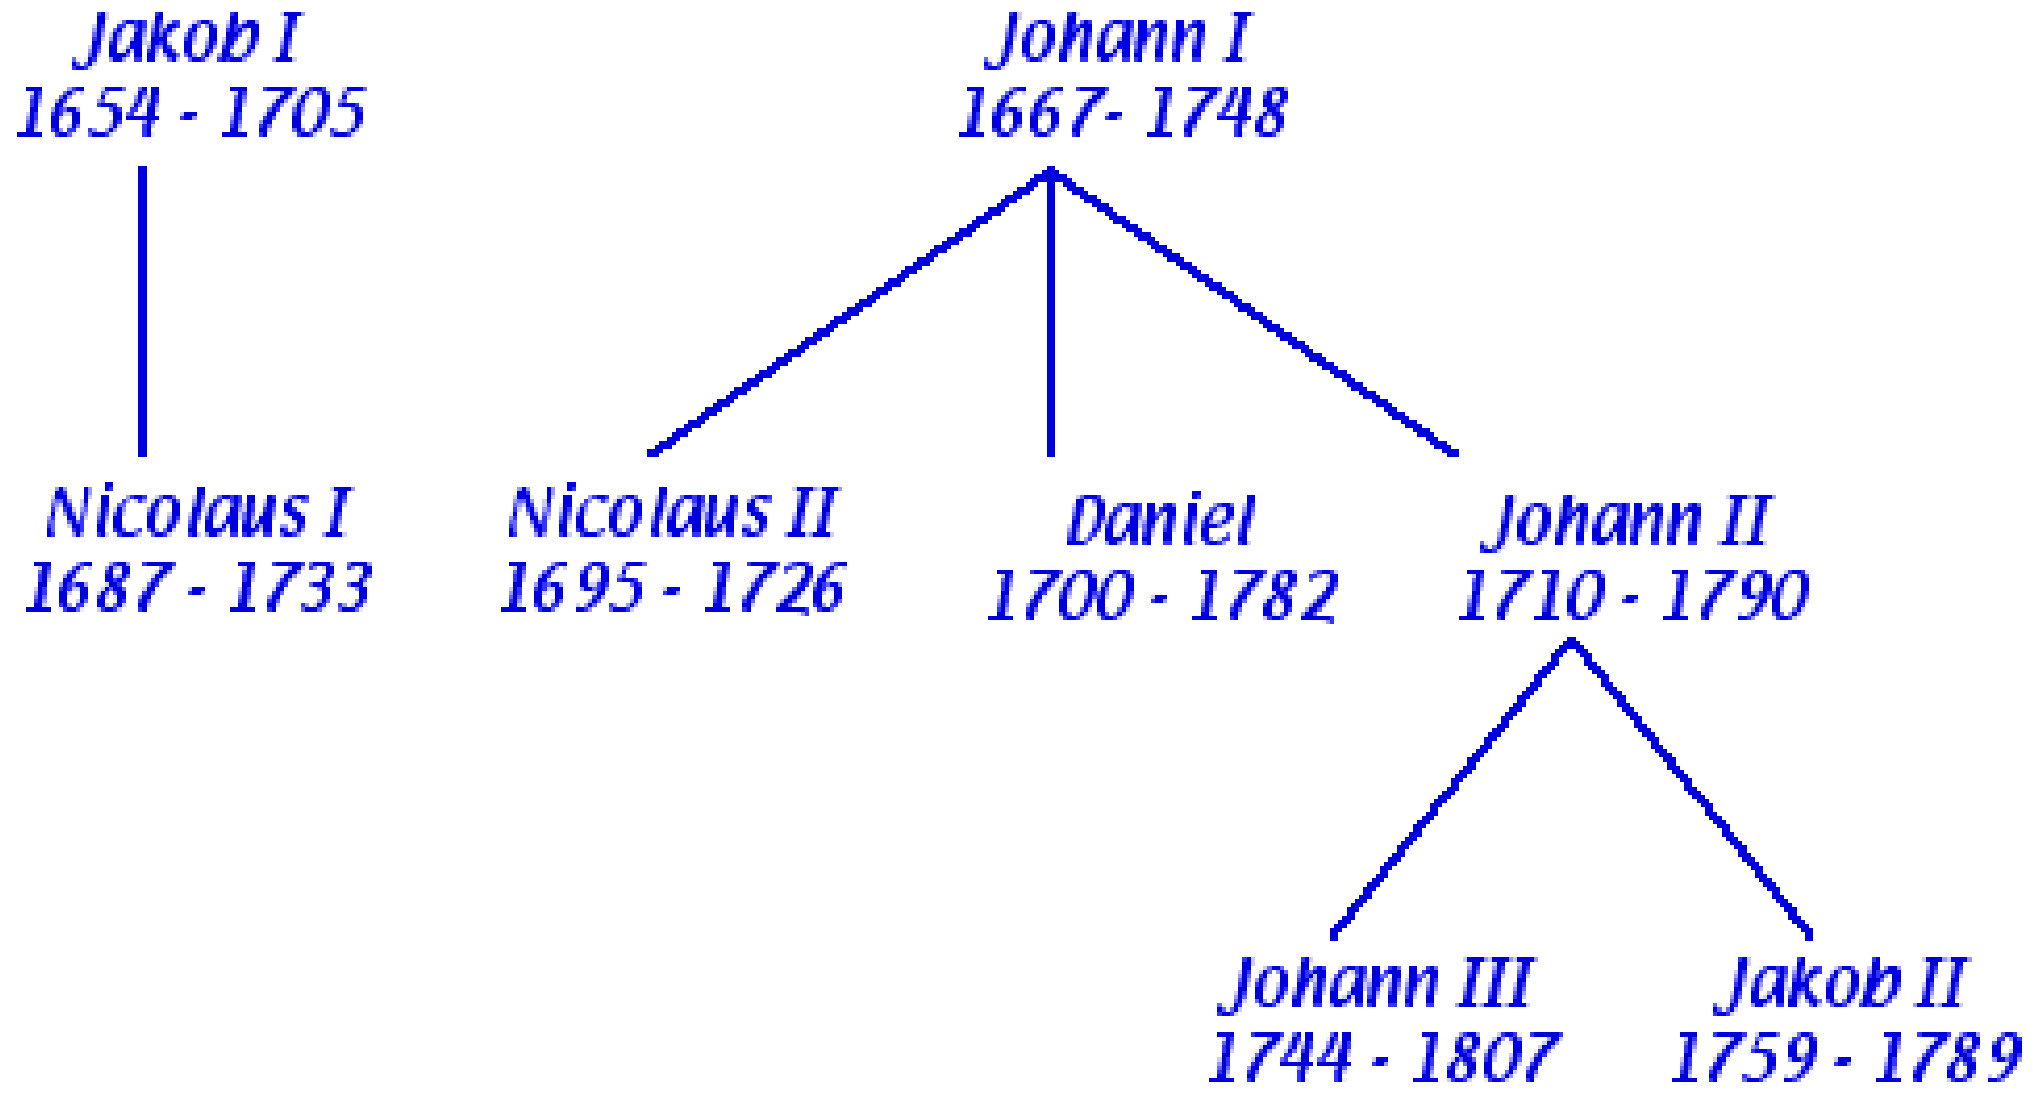
\includegraphics[scale=0.6]{Bernoulli_family} }


\end{frame}



\begin{frame}[fragile]\frametitle{The Bernoulli family}

$X = \{0,1\}$ \\
$$p(x;\alpha) = \left\{\begin{array}{ll}
			1-\alpha & \mbox{if } x =0 \\
			\alpha & \mbox{if } x=1
						   .	\end{array}
						\right.  	
$$


\end{frame}



\begin{frame}[fragile]\frametitle{The Bernoulli family}

\center{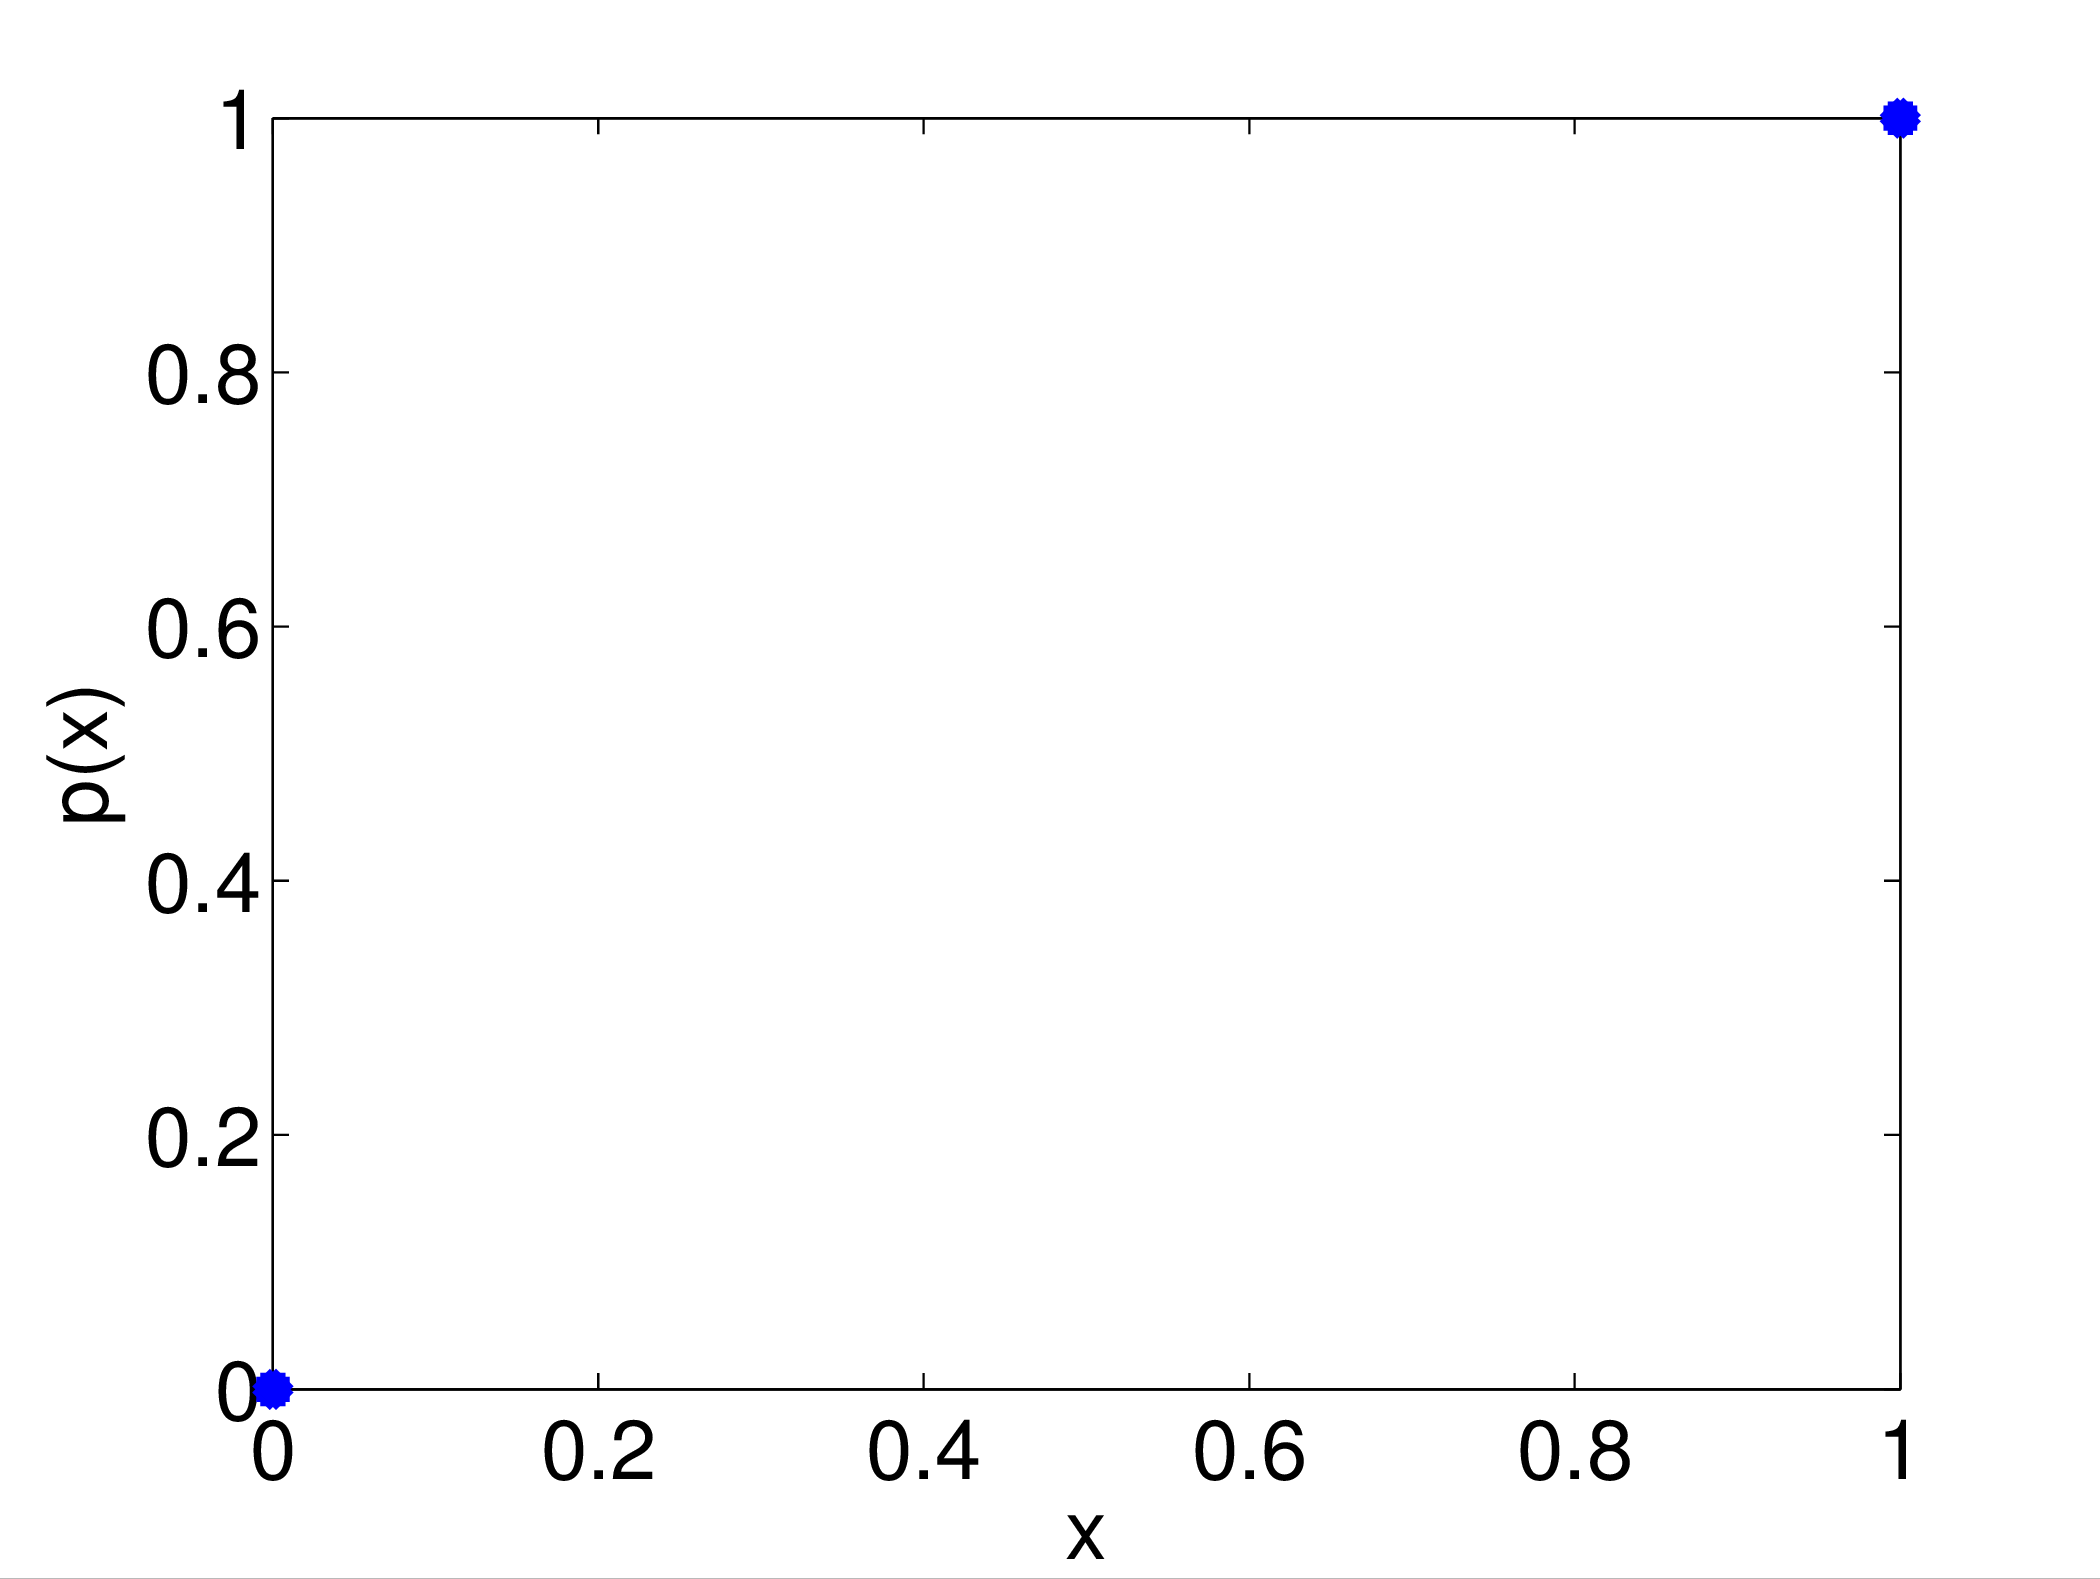
\includegraphics[scale=0.4]{image1} }


\end{frame}

\begin{frame}[fragile]\frametitle{The Bernoulli family}

\center{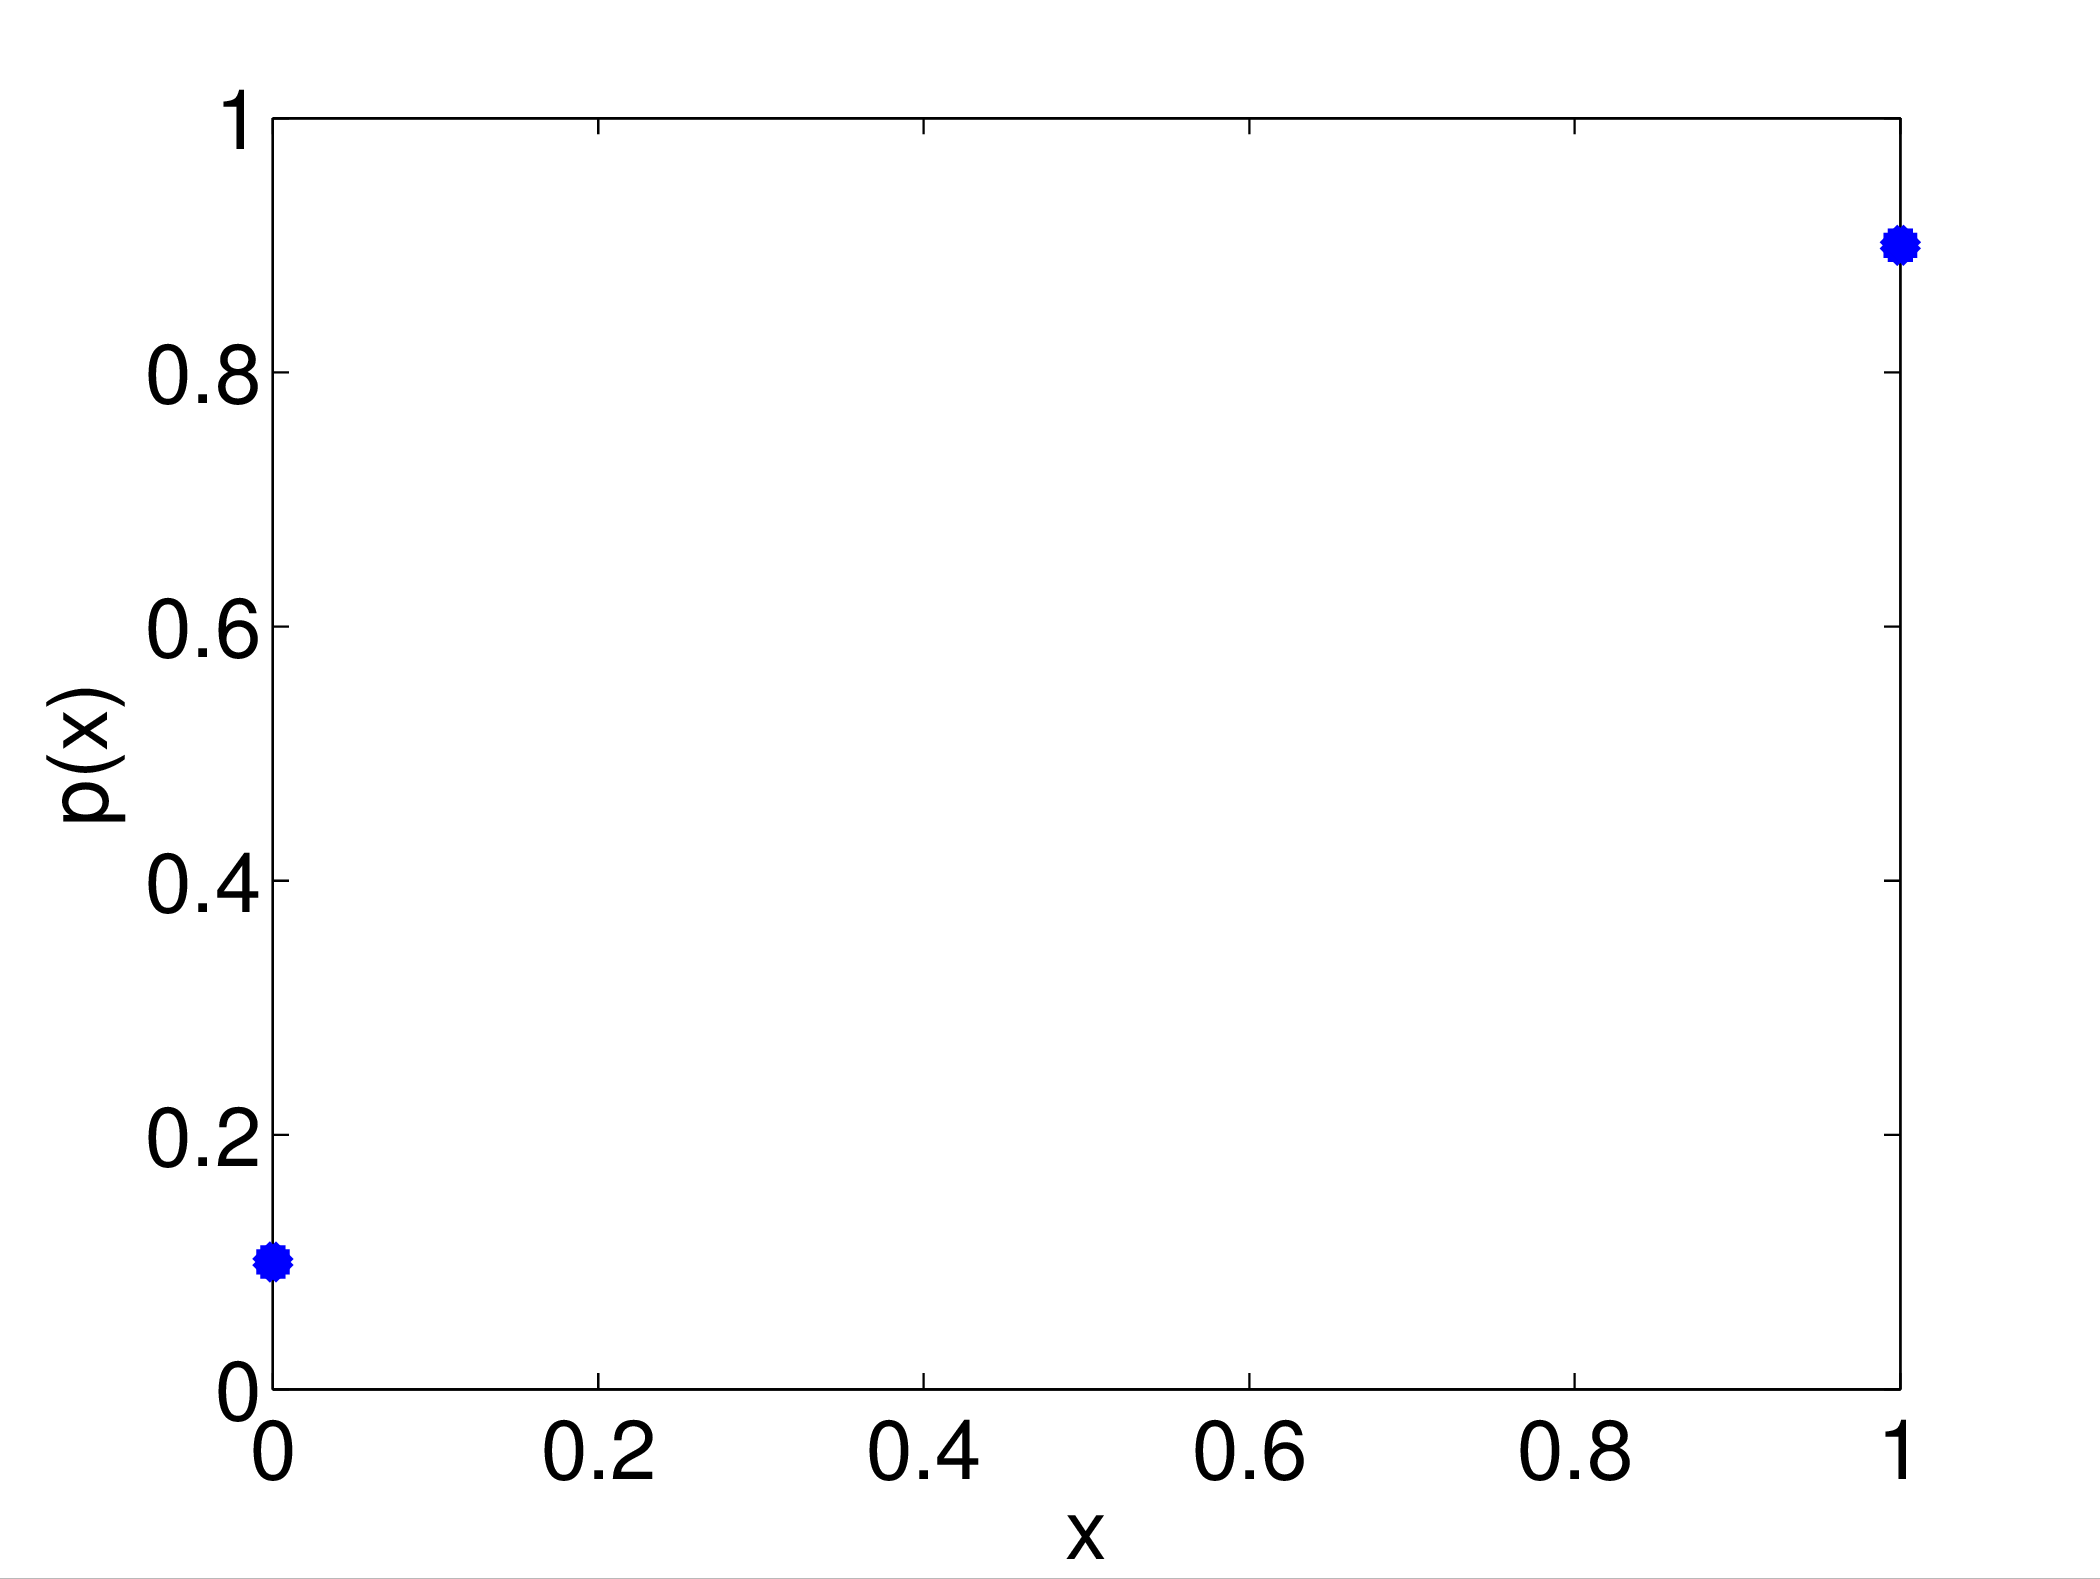
\includegraphics[scale=0.4]{image2} }


\end{frame}

\begin{frame}[fragile]\frametitle{The Bernoulli family}

\center{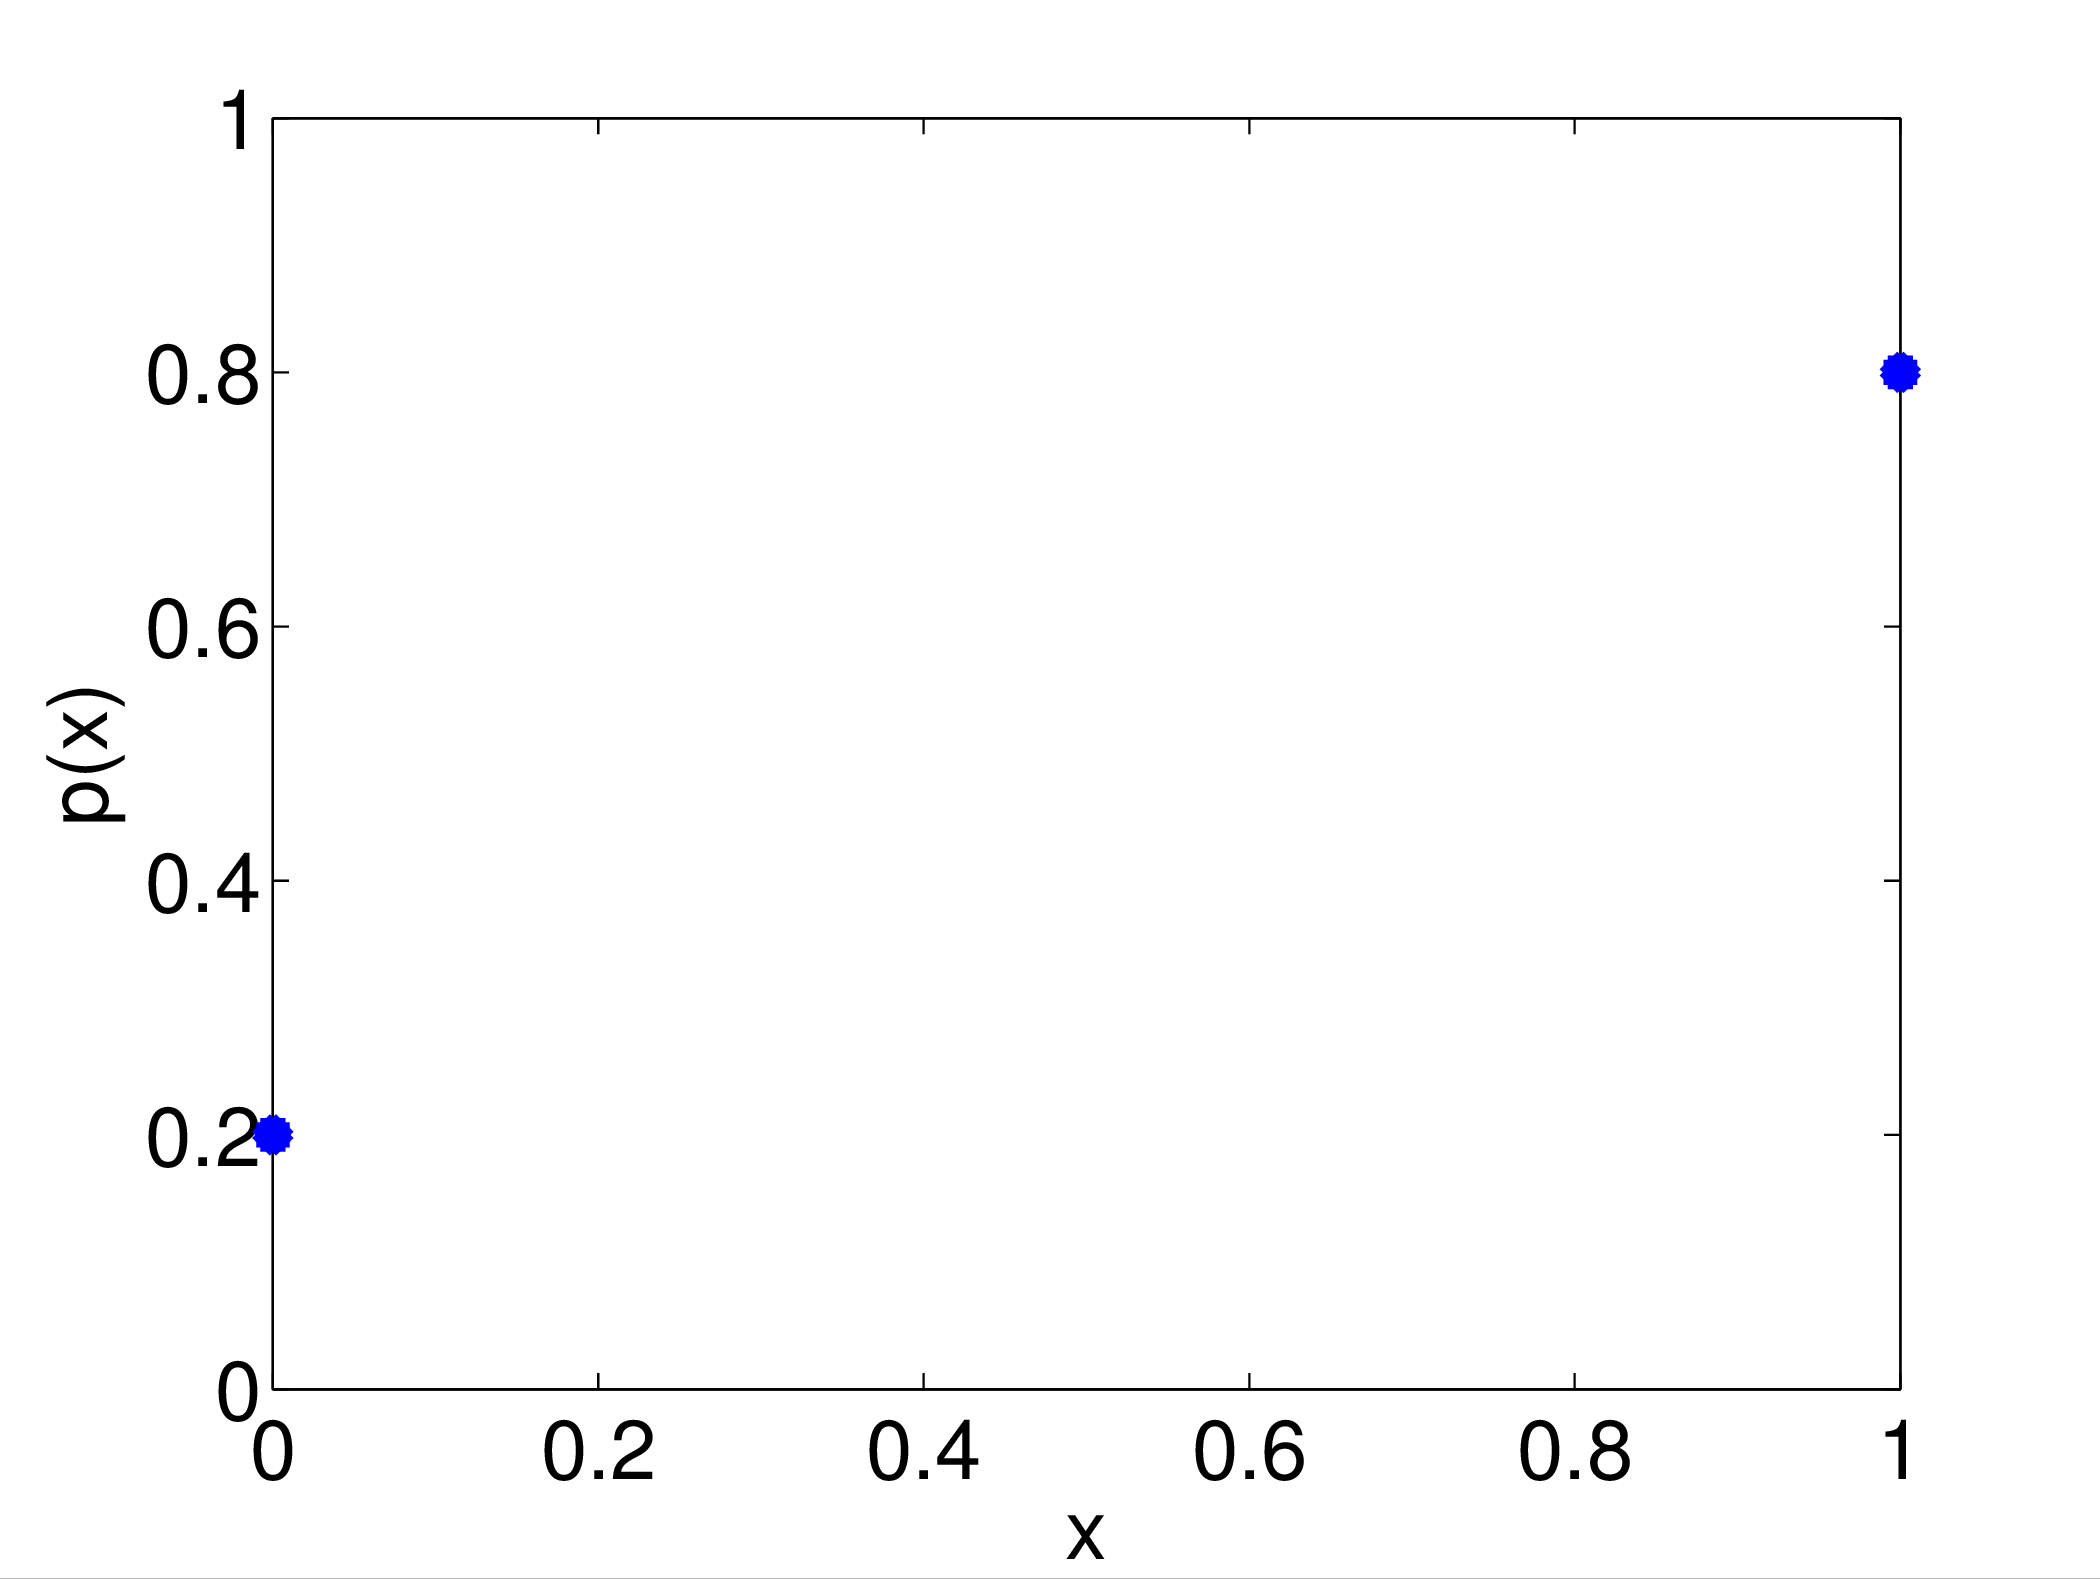
\includegraphics[scale=0.4]{image3} }


\end{frame}

\begin{frame}[fragile]\frametitle{The Bernoulli family}

\center{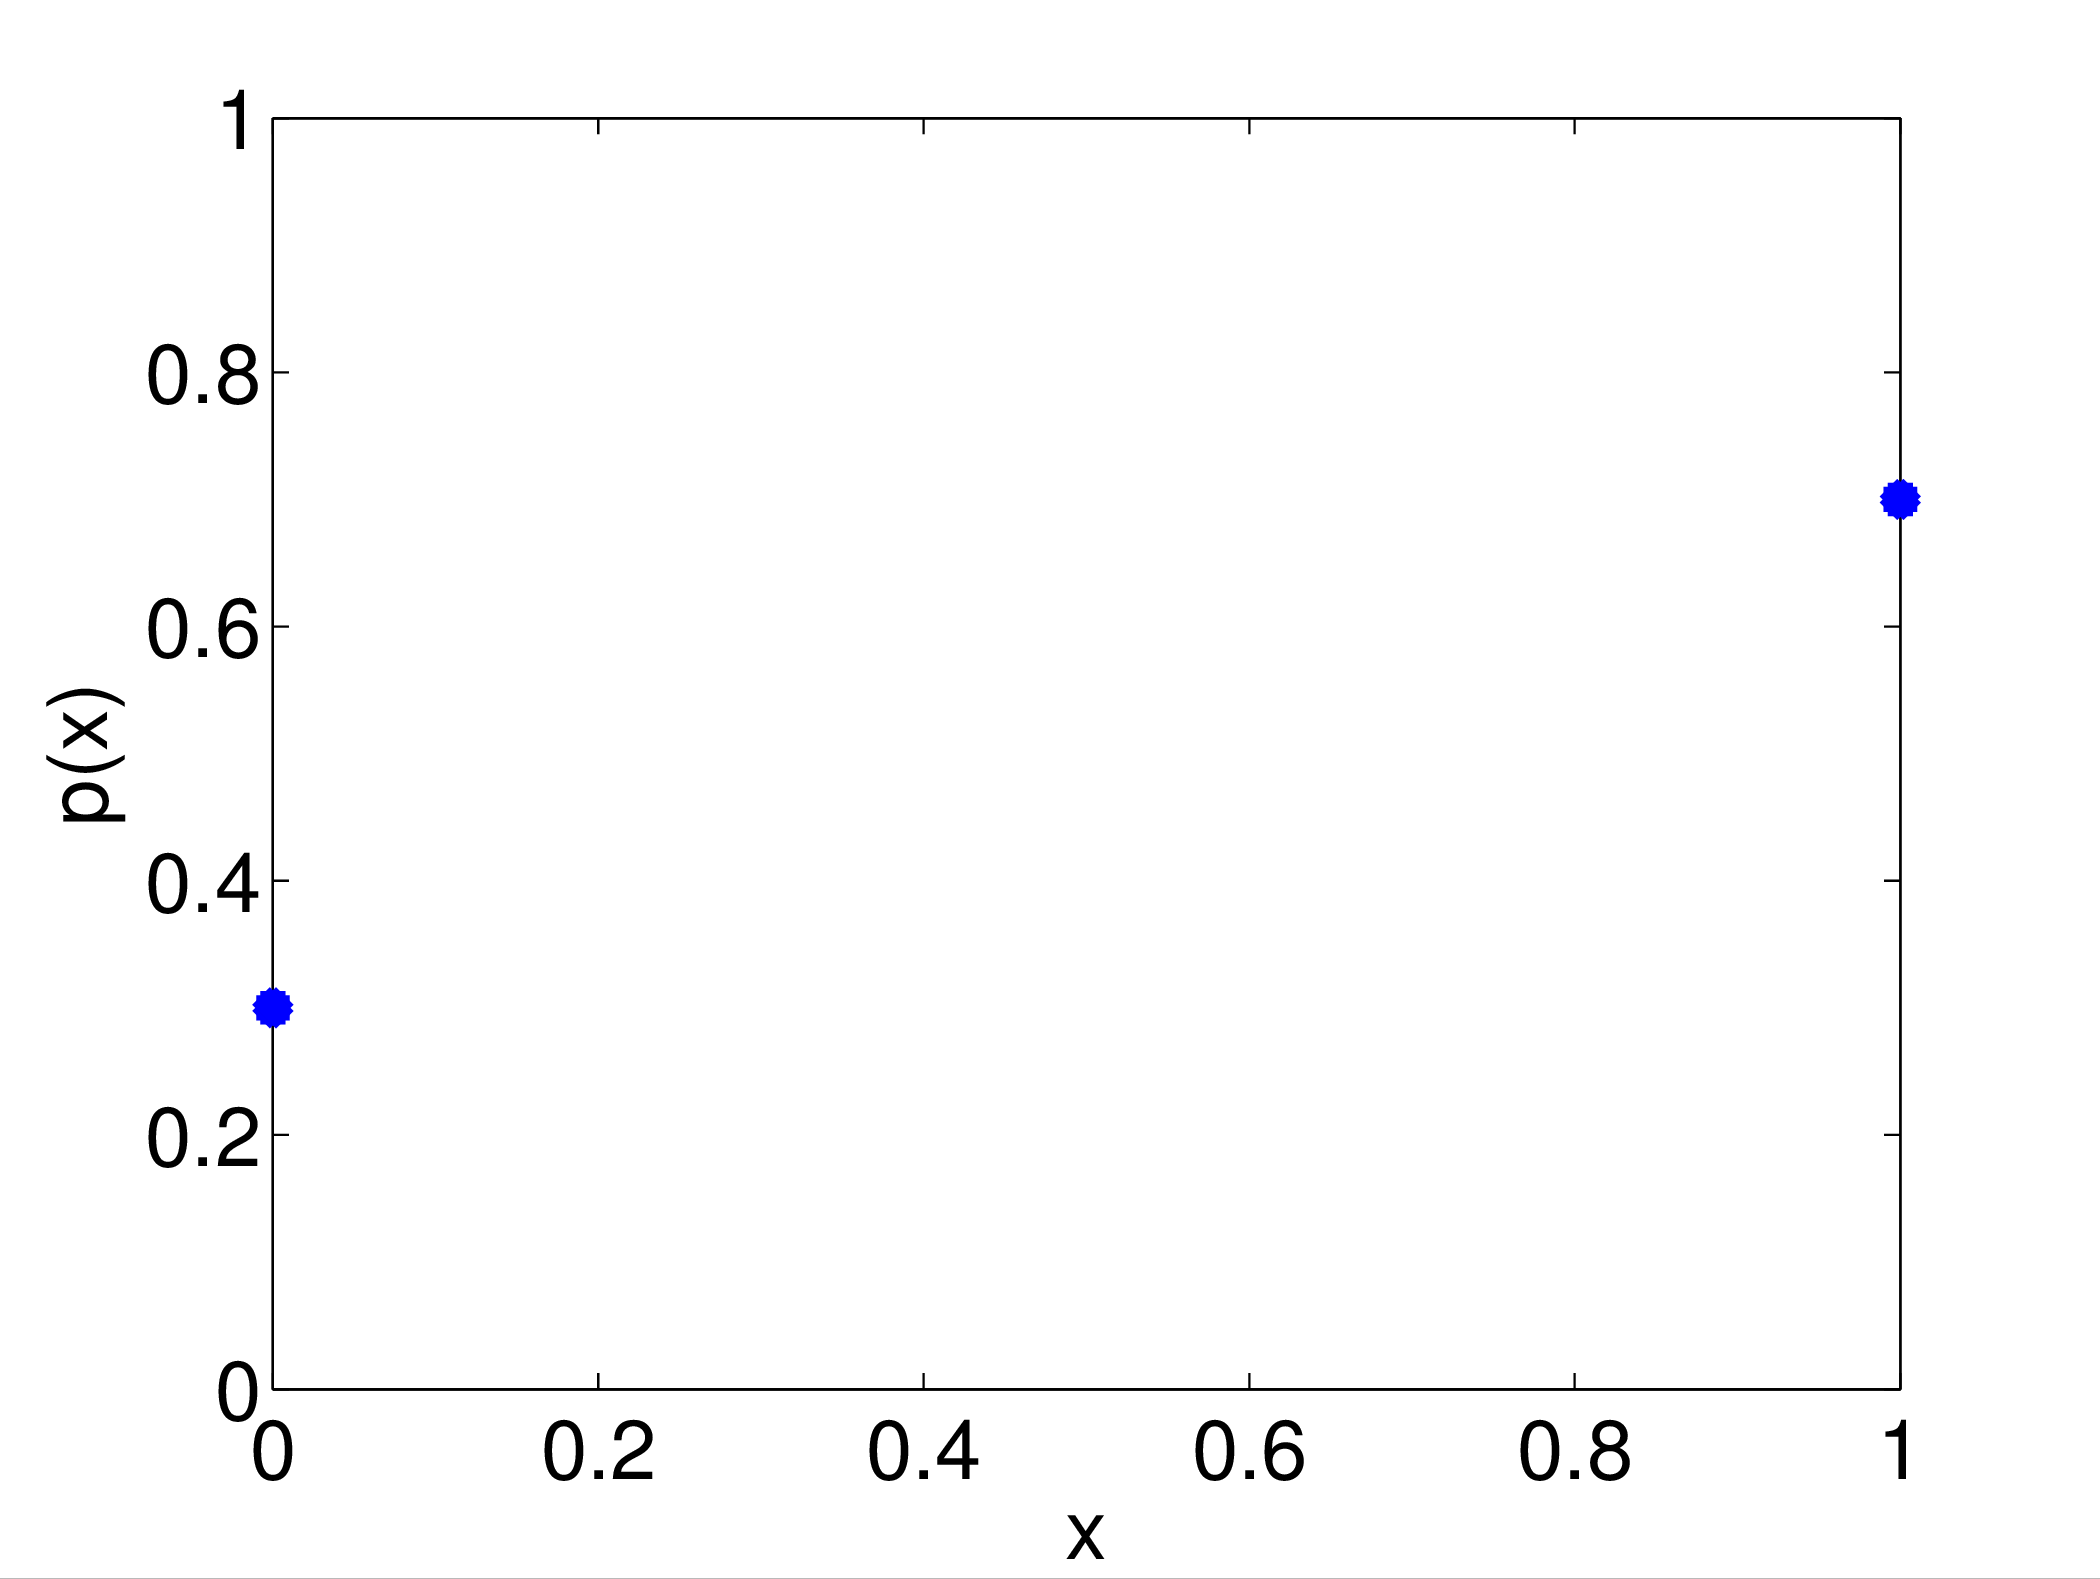
\includegraphics[scale=0.4]{image4} }


\end{frame}

\begin{frame}[fragile]\frametitle{The Bernoulli family}

\center{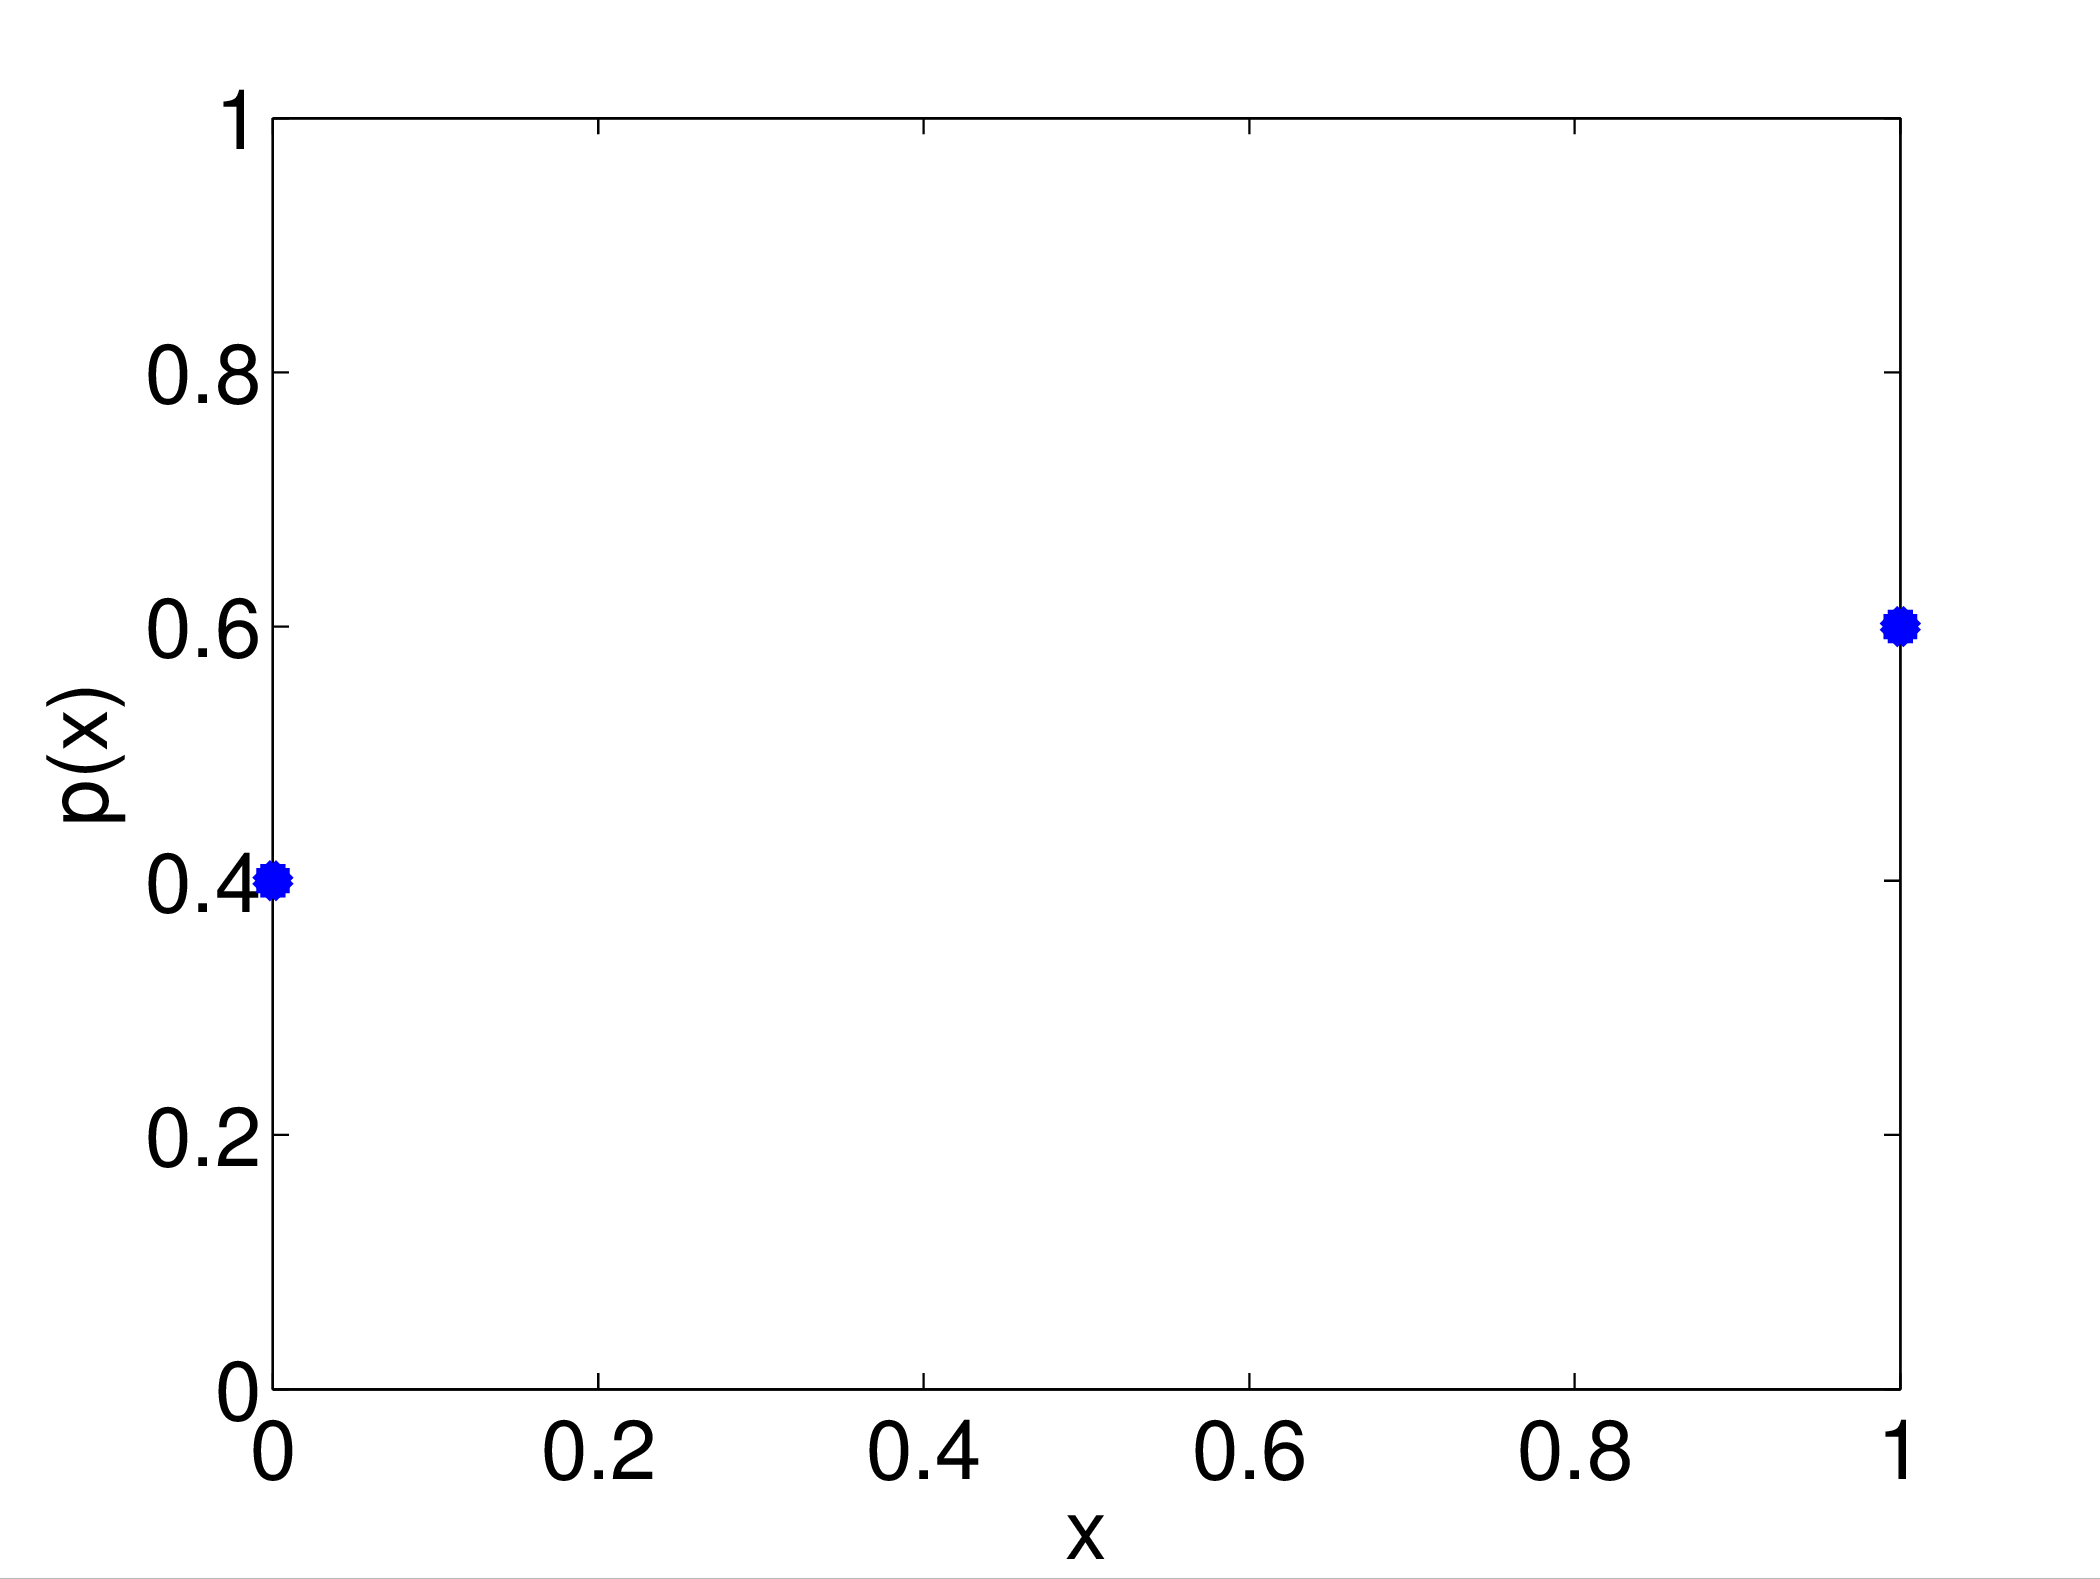
\includegraphics[scale=0.4]{image5} }

\end{frame}

\begin{frame}[fragile]\frametitle{The Bernoulli family}

\center{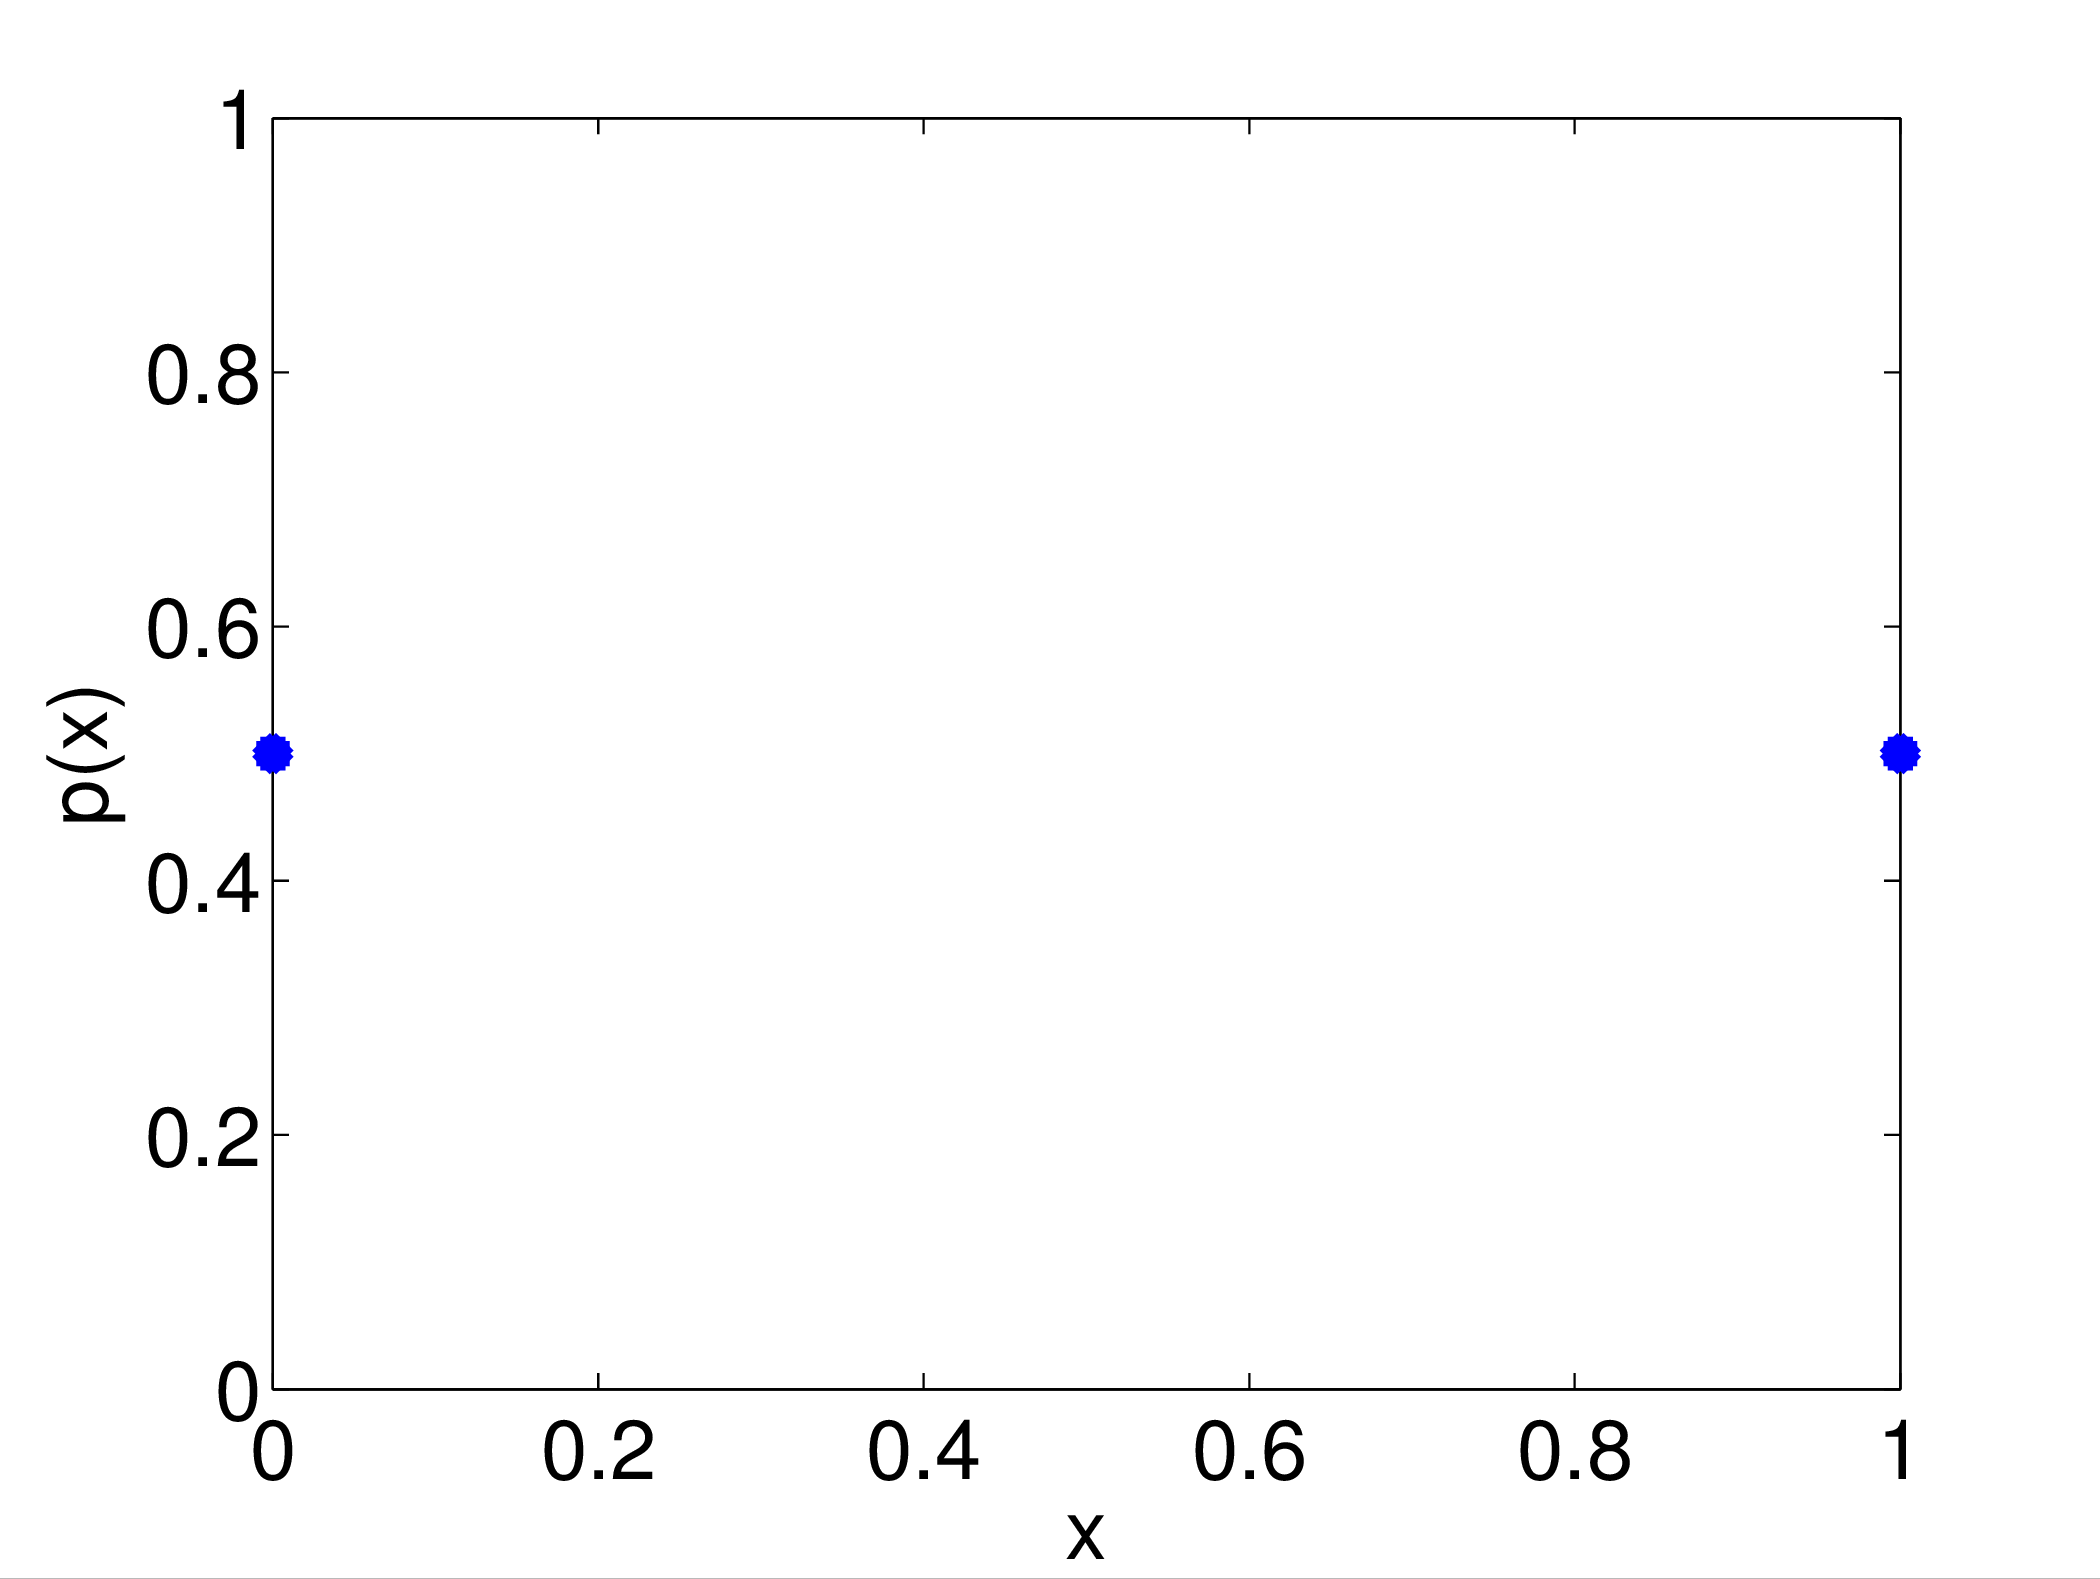
\includegraphics[scale=0.4]{image6} }


\end{frame}

\begin{frame}[fragile]\frametitle{The Bernoulli family}

\center{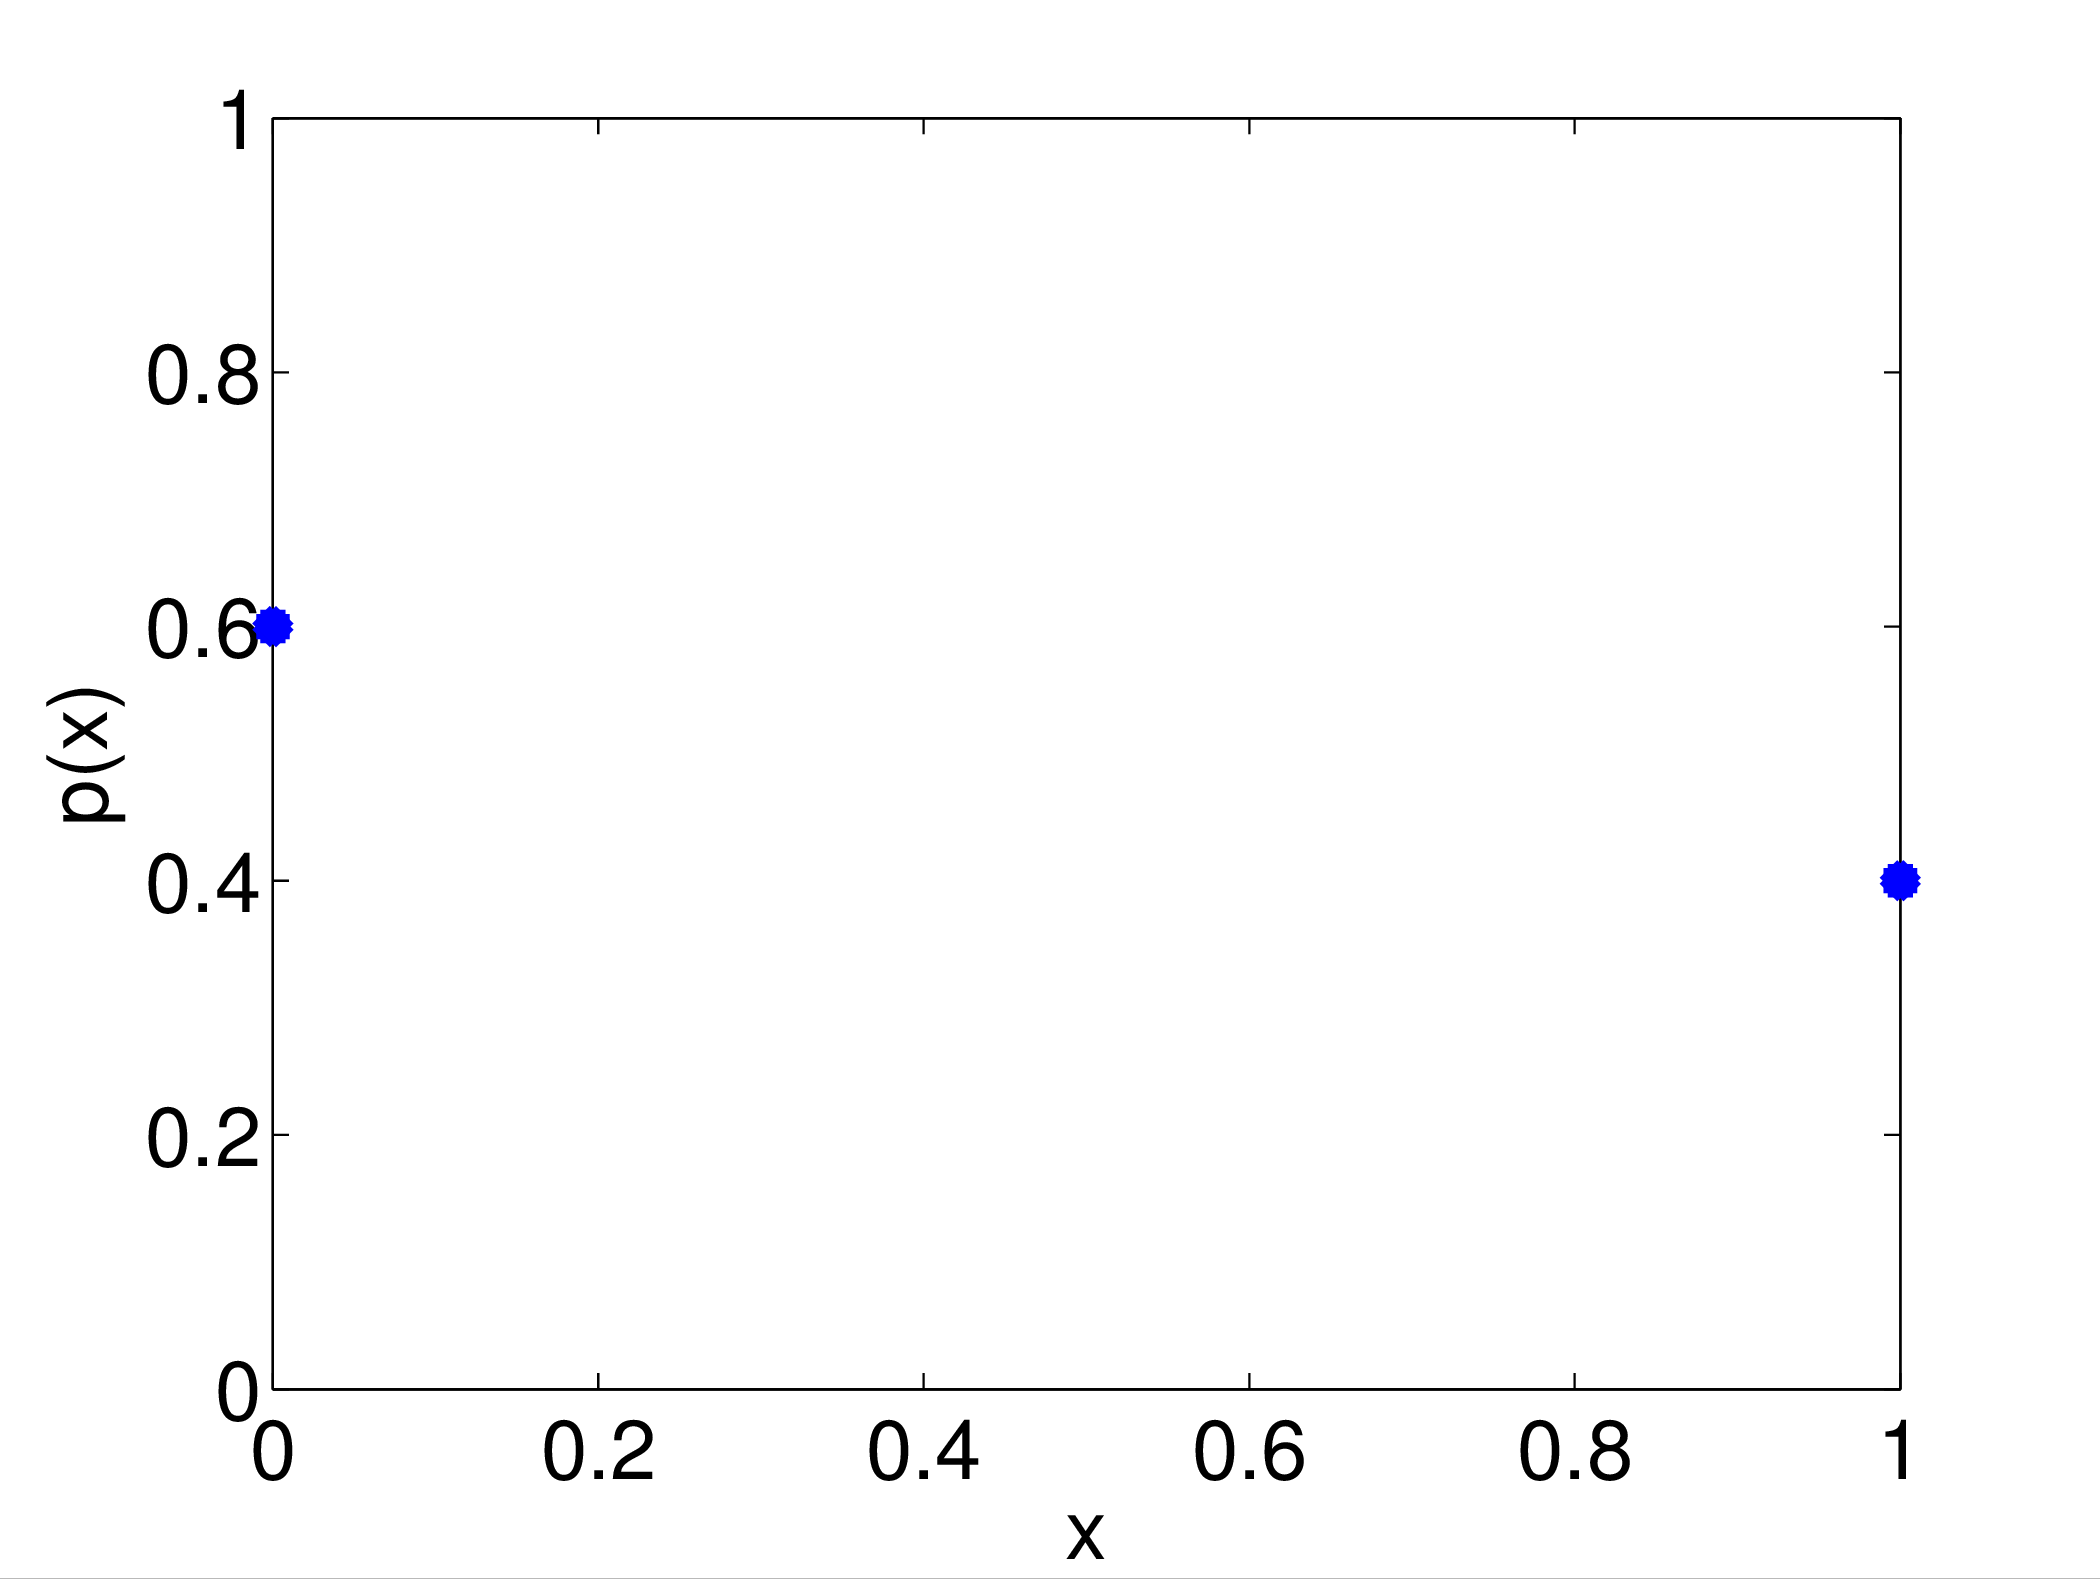
\includegraphics[scale=0.4]{image7} }


\end{frame}

\begin{frame}[fragile]\frametitle{The Bernoulli family}

\center{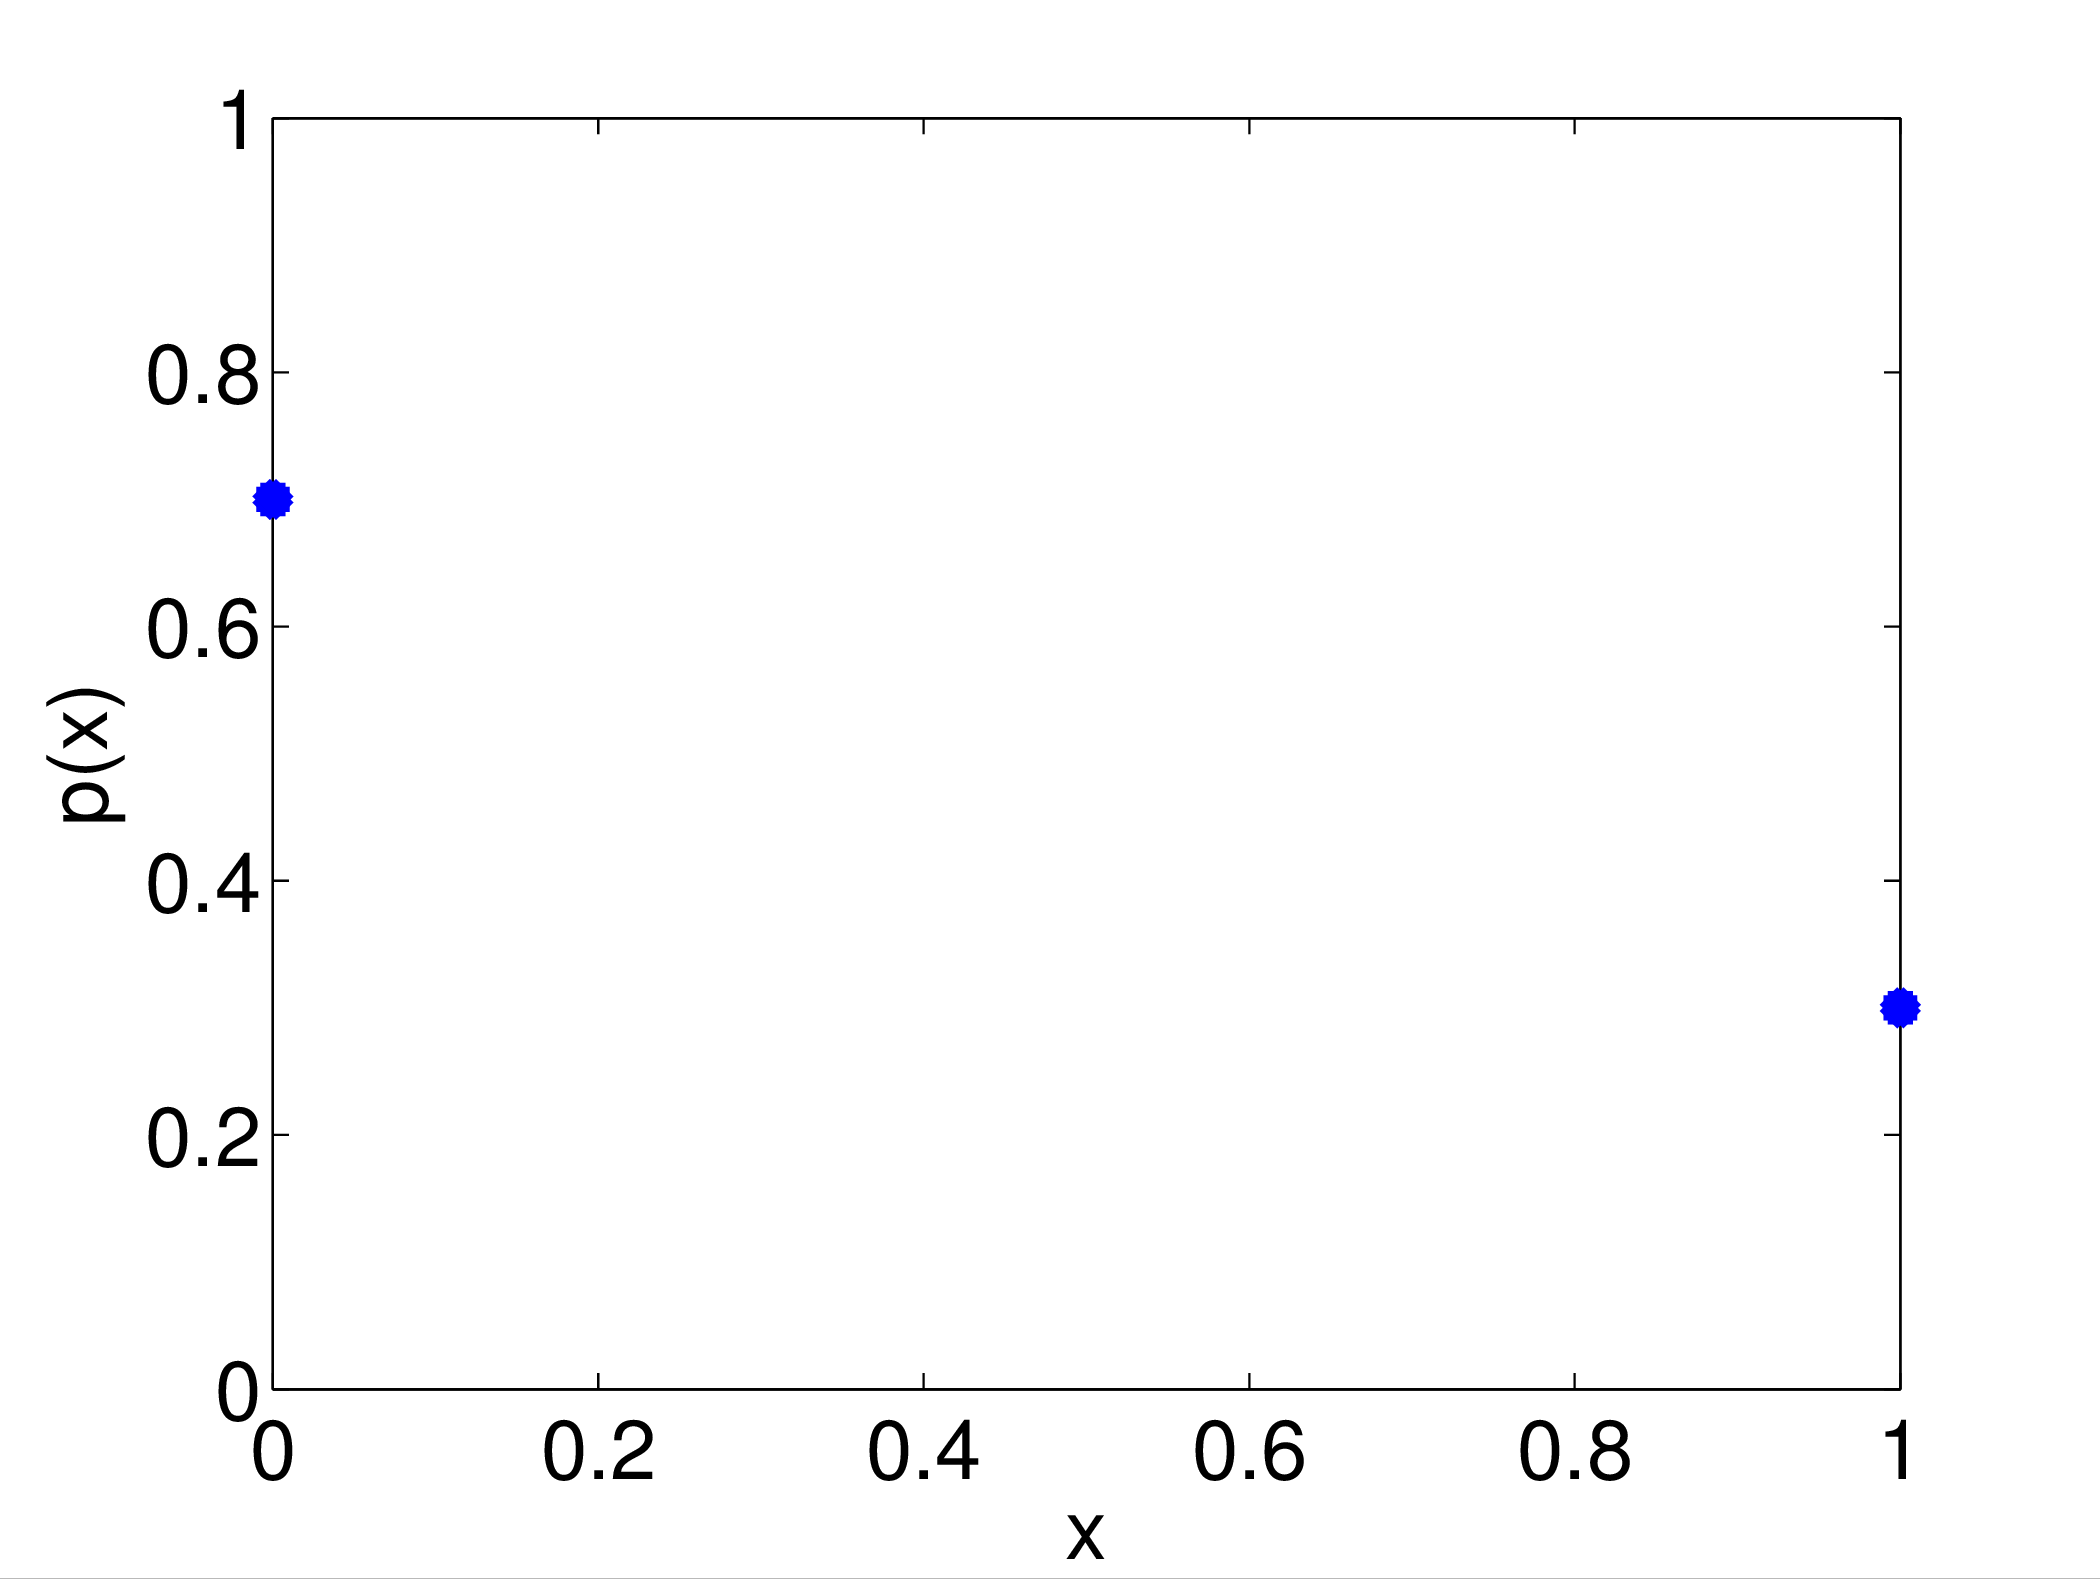
\includegraphics[scale=0.4]{image8} }


\end{frame}

\begin{frame}[fragile]\frametitle{The Bernoulli family}

\center{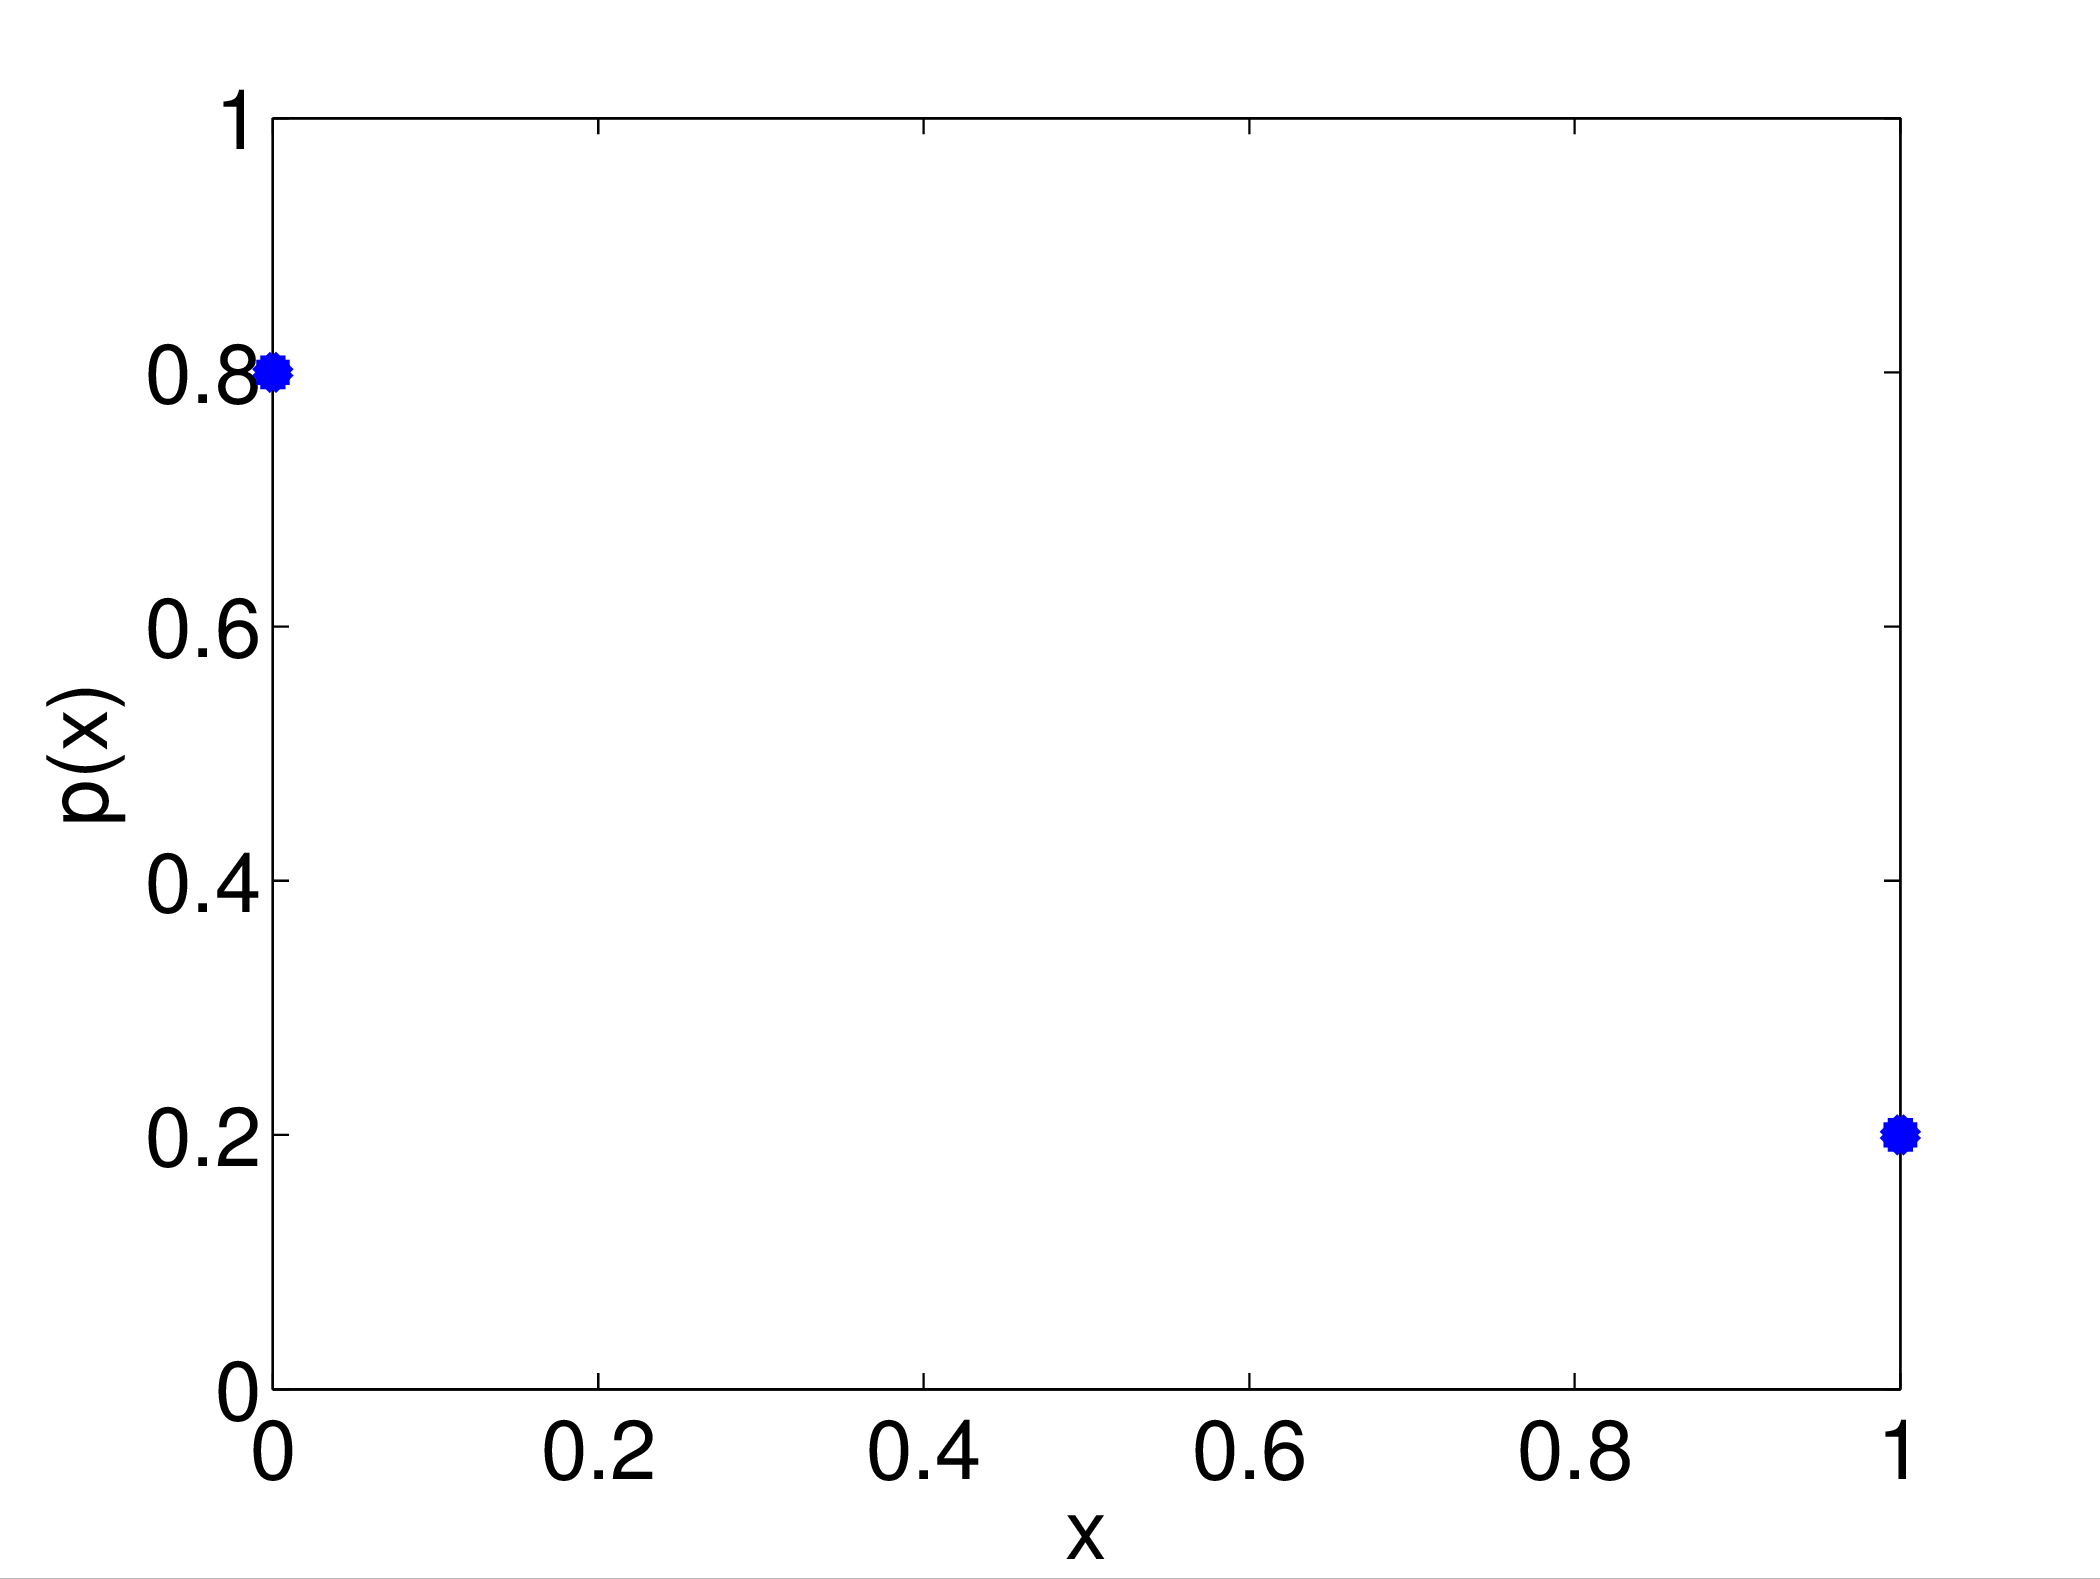
\includegraphics[scale=0.4]{image9} }


\end{frame}

\begin{frame}[fragile]\frametitle{The Bernoulli family}

\center{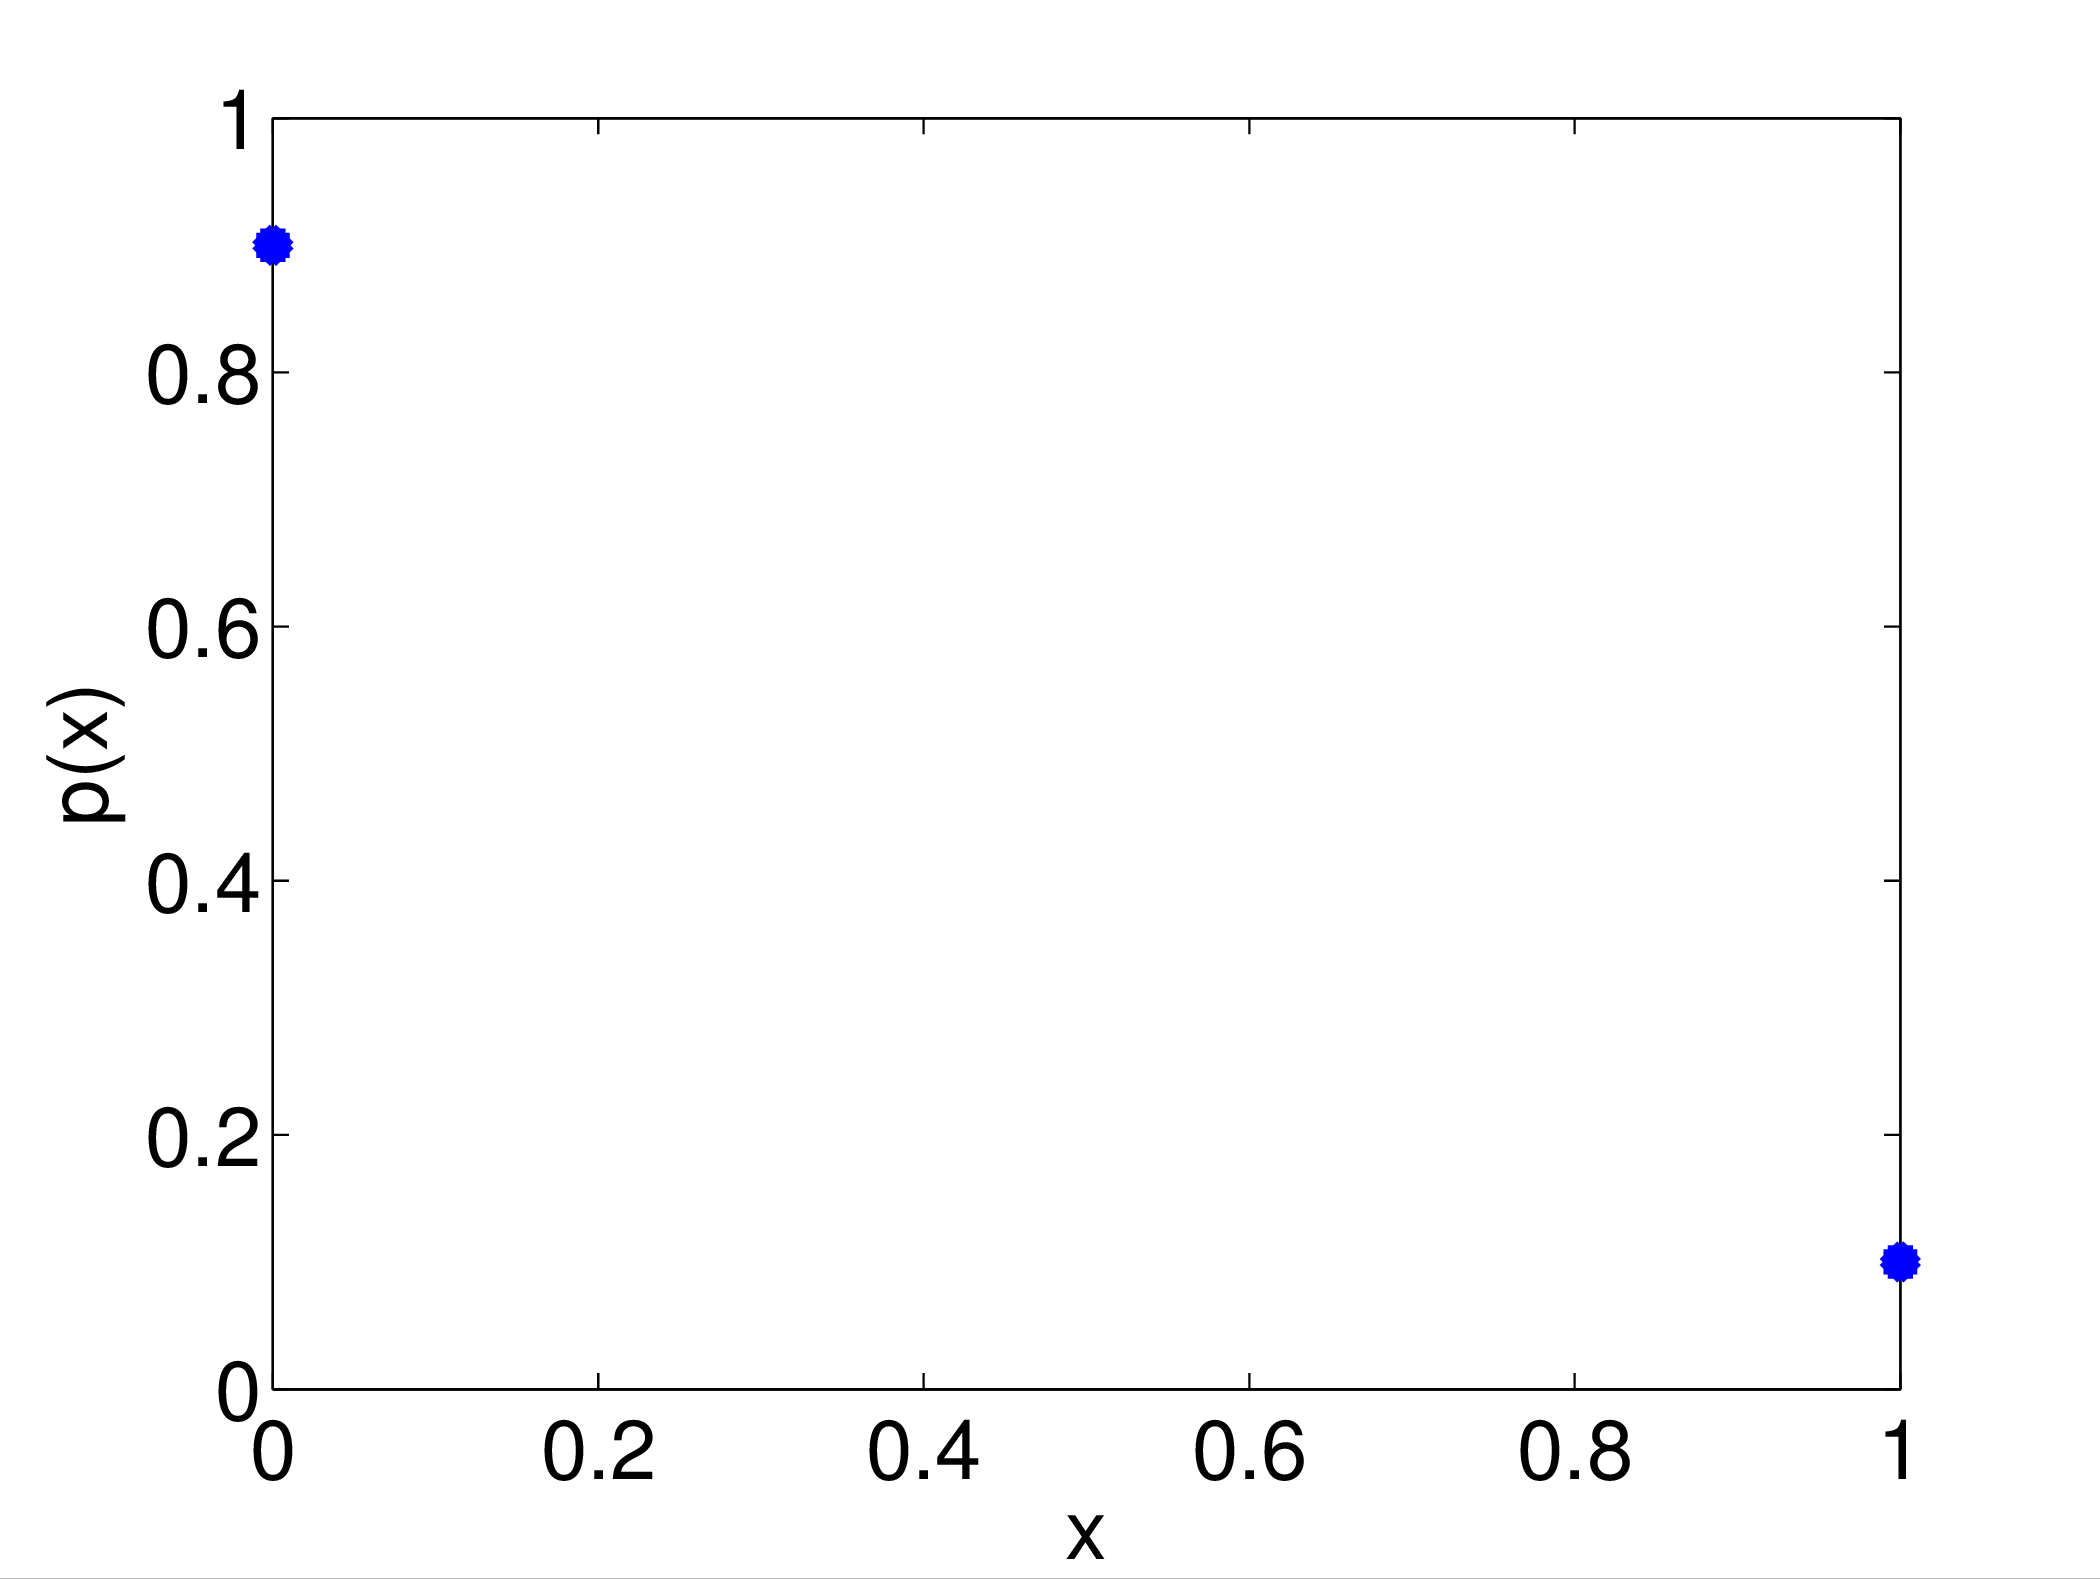
\includegraphics[scale=0.4]{image10} }


\end{frame}

\begin{frame}[fragile]\frametitle{The Bernoulli family}

\center{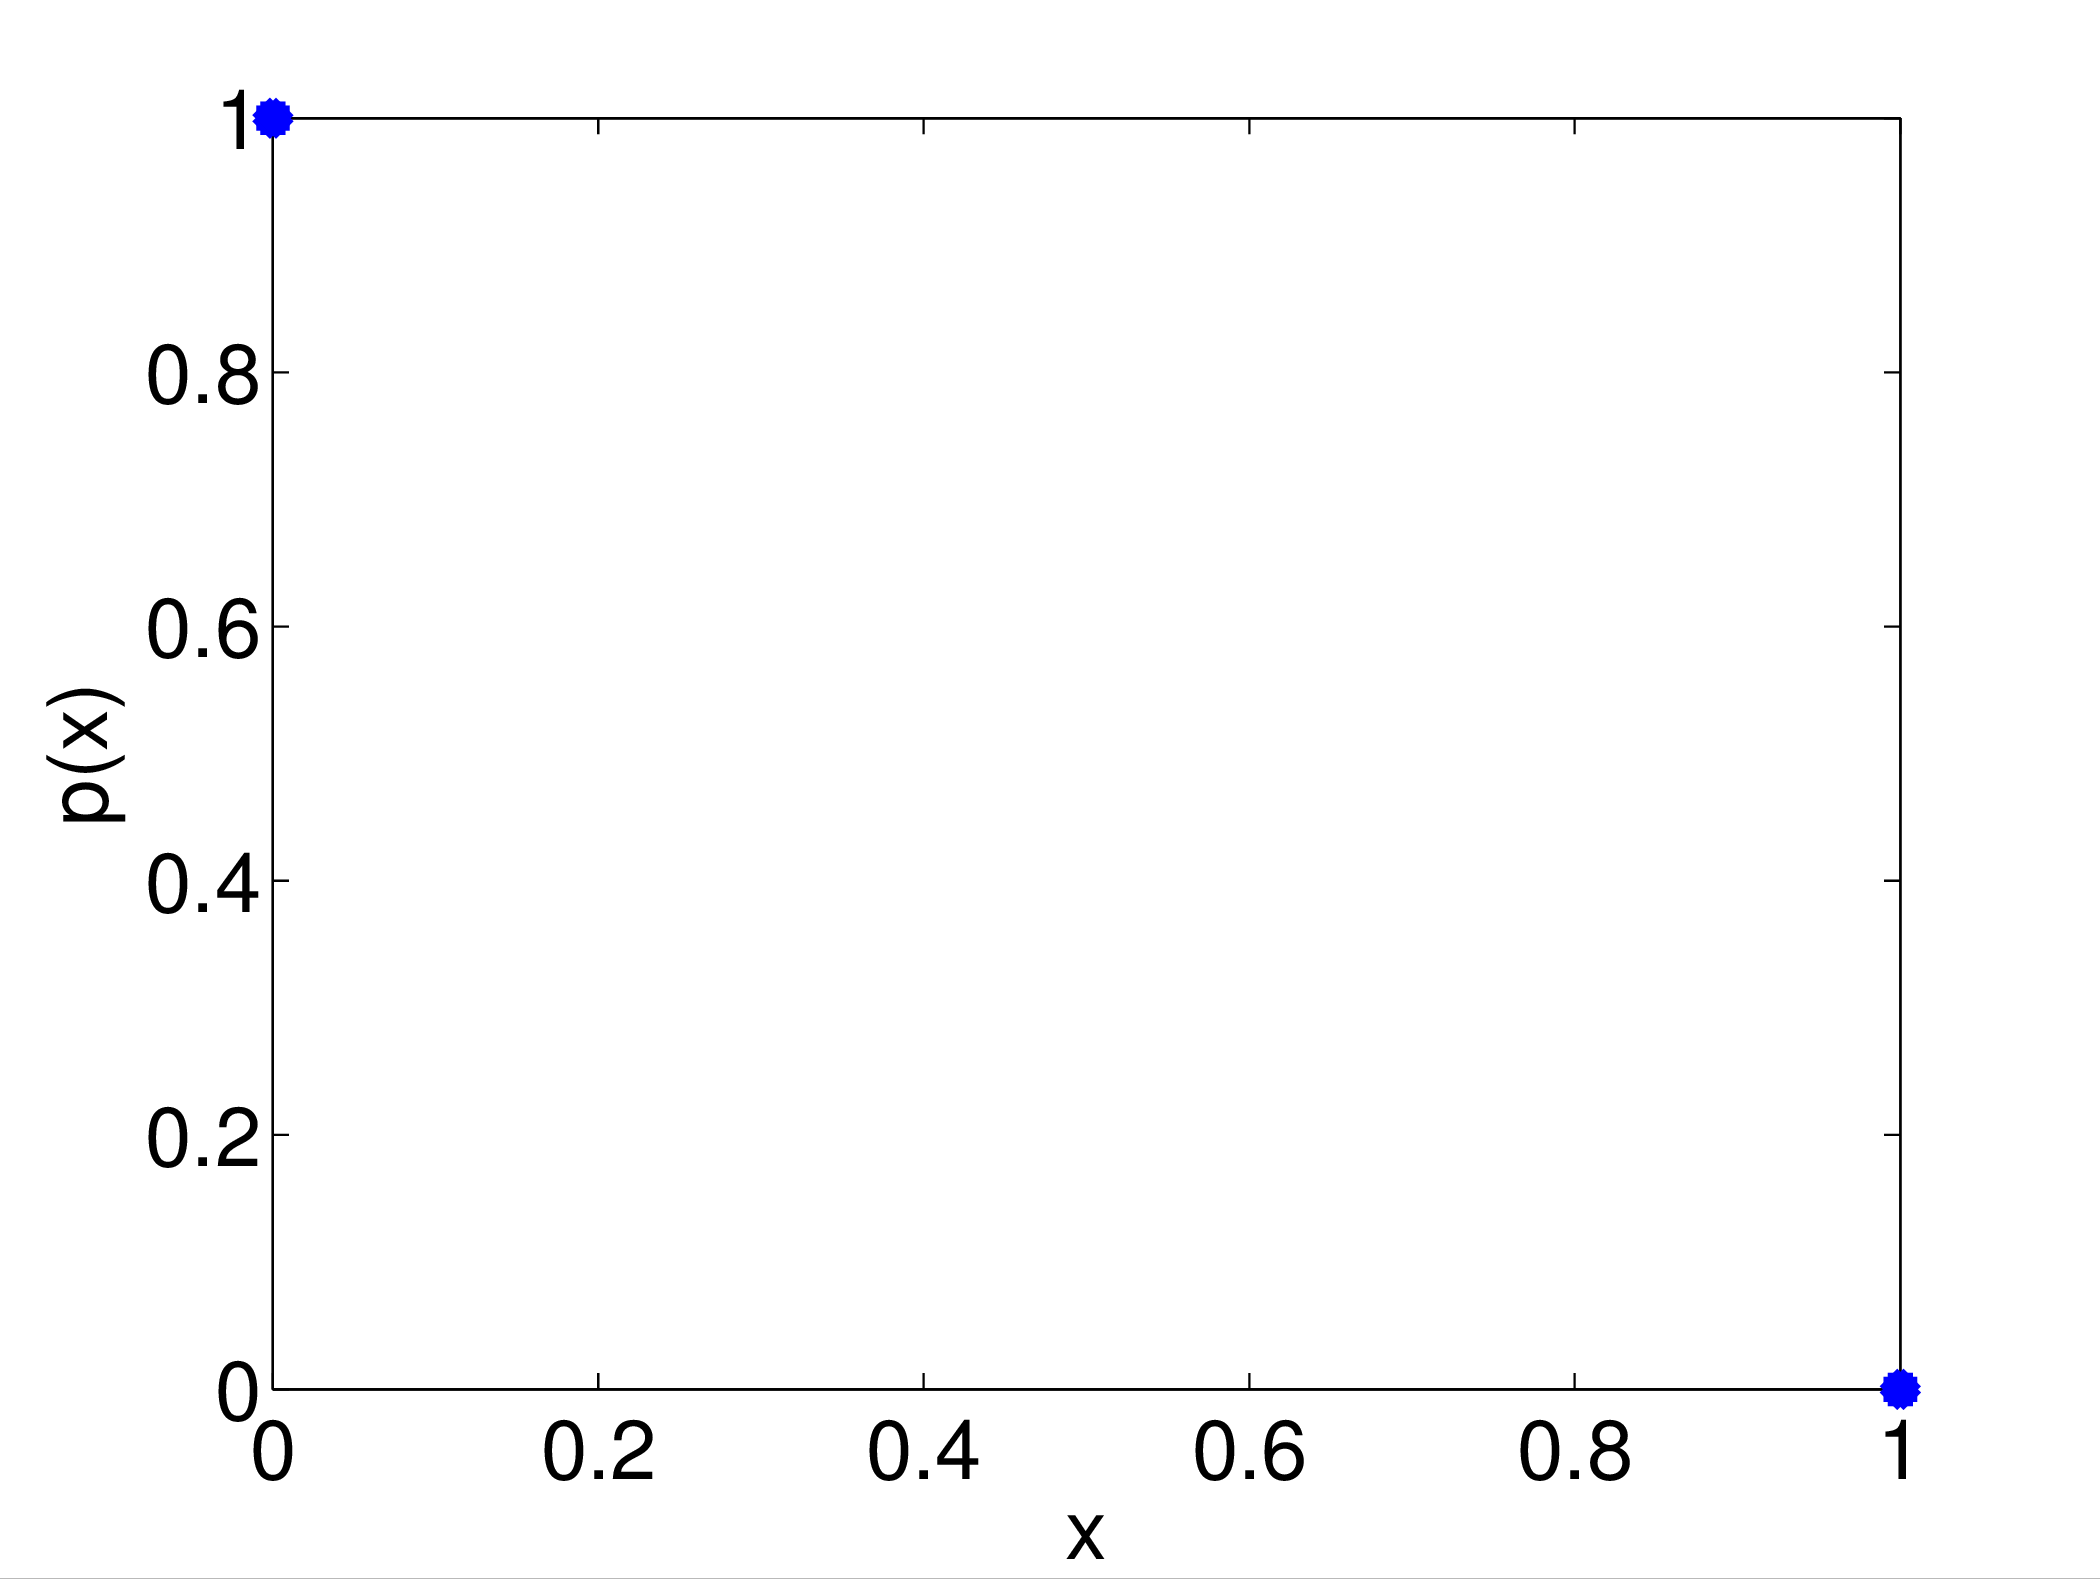
\includegraphics[scale=0.4]{image11} }


\end{frame}


\begin{frame}[fragile]\frametitle{Matlab code}

\begin{tabbing}
for \= i = 0:10\\
\> figure(i+1);\\  
\>  alpha = i*.1;\\
\>  x=[0,1];\\
\>  y=[alpha,1-alpha];\\
\>  plot(x,y,'*','LineWidth',8);\\ 
\>  h=gca;\\
\>  set(h,'FontSize',[20]);\\
\>  set(h,'YLim',[0 1]);\\
\>  set(h,'XLim',[0 1]);\\
\>  xlabel('x');  \\
\>  ylabel('p(x)'); \\
end
\end{tabbing}

\end{frame}



\begin{frame}[fragile]\frametitle{Pregnancy}

Suppose a couple is trying to get pregnant. \\ 

Let the number of months be the random variable $X$ and let
the probability of conception be $p$. 
\begin{eqnarray*}
\pr(x=1) &=& \pr(S) = p \\ 
\pr(x=2) &=& \pr(FS) = (1-p)p  \\ 
\pr(x=3) &=& \pr(FFS) = (1-p)^{2}p  
\end{eqnarray*}
or
$$p(x) = (1-p)^{x-1}p, \, \, \, \, \, \, \, x=1,2,3,...$$


\end{frame}


\begin{frame}[fragile]\frametitle{Cumulative distribution function}

\begin{defn}
The {\bf cumulative distribution function} (cdf) $F(x)$ of
a rv $X$ with pdf $p(x)$ is defined as
$$F(x) = \pr(X \leq x) = \sum_{i=1}^x p(i).$$
So for any number $x$, $F(x)$ is the probability that the
observed value of $X$ is at most $x$.
\end{defn}

\end{frame}



\begin{frame}[fragile]\frametitle{An example}

\center{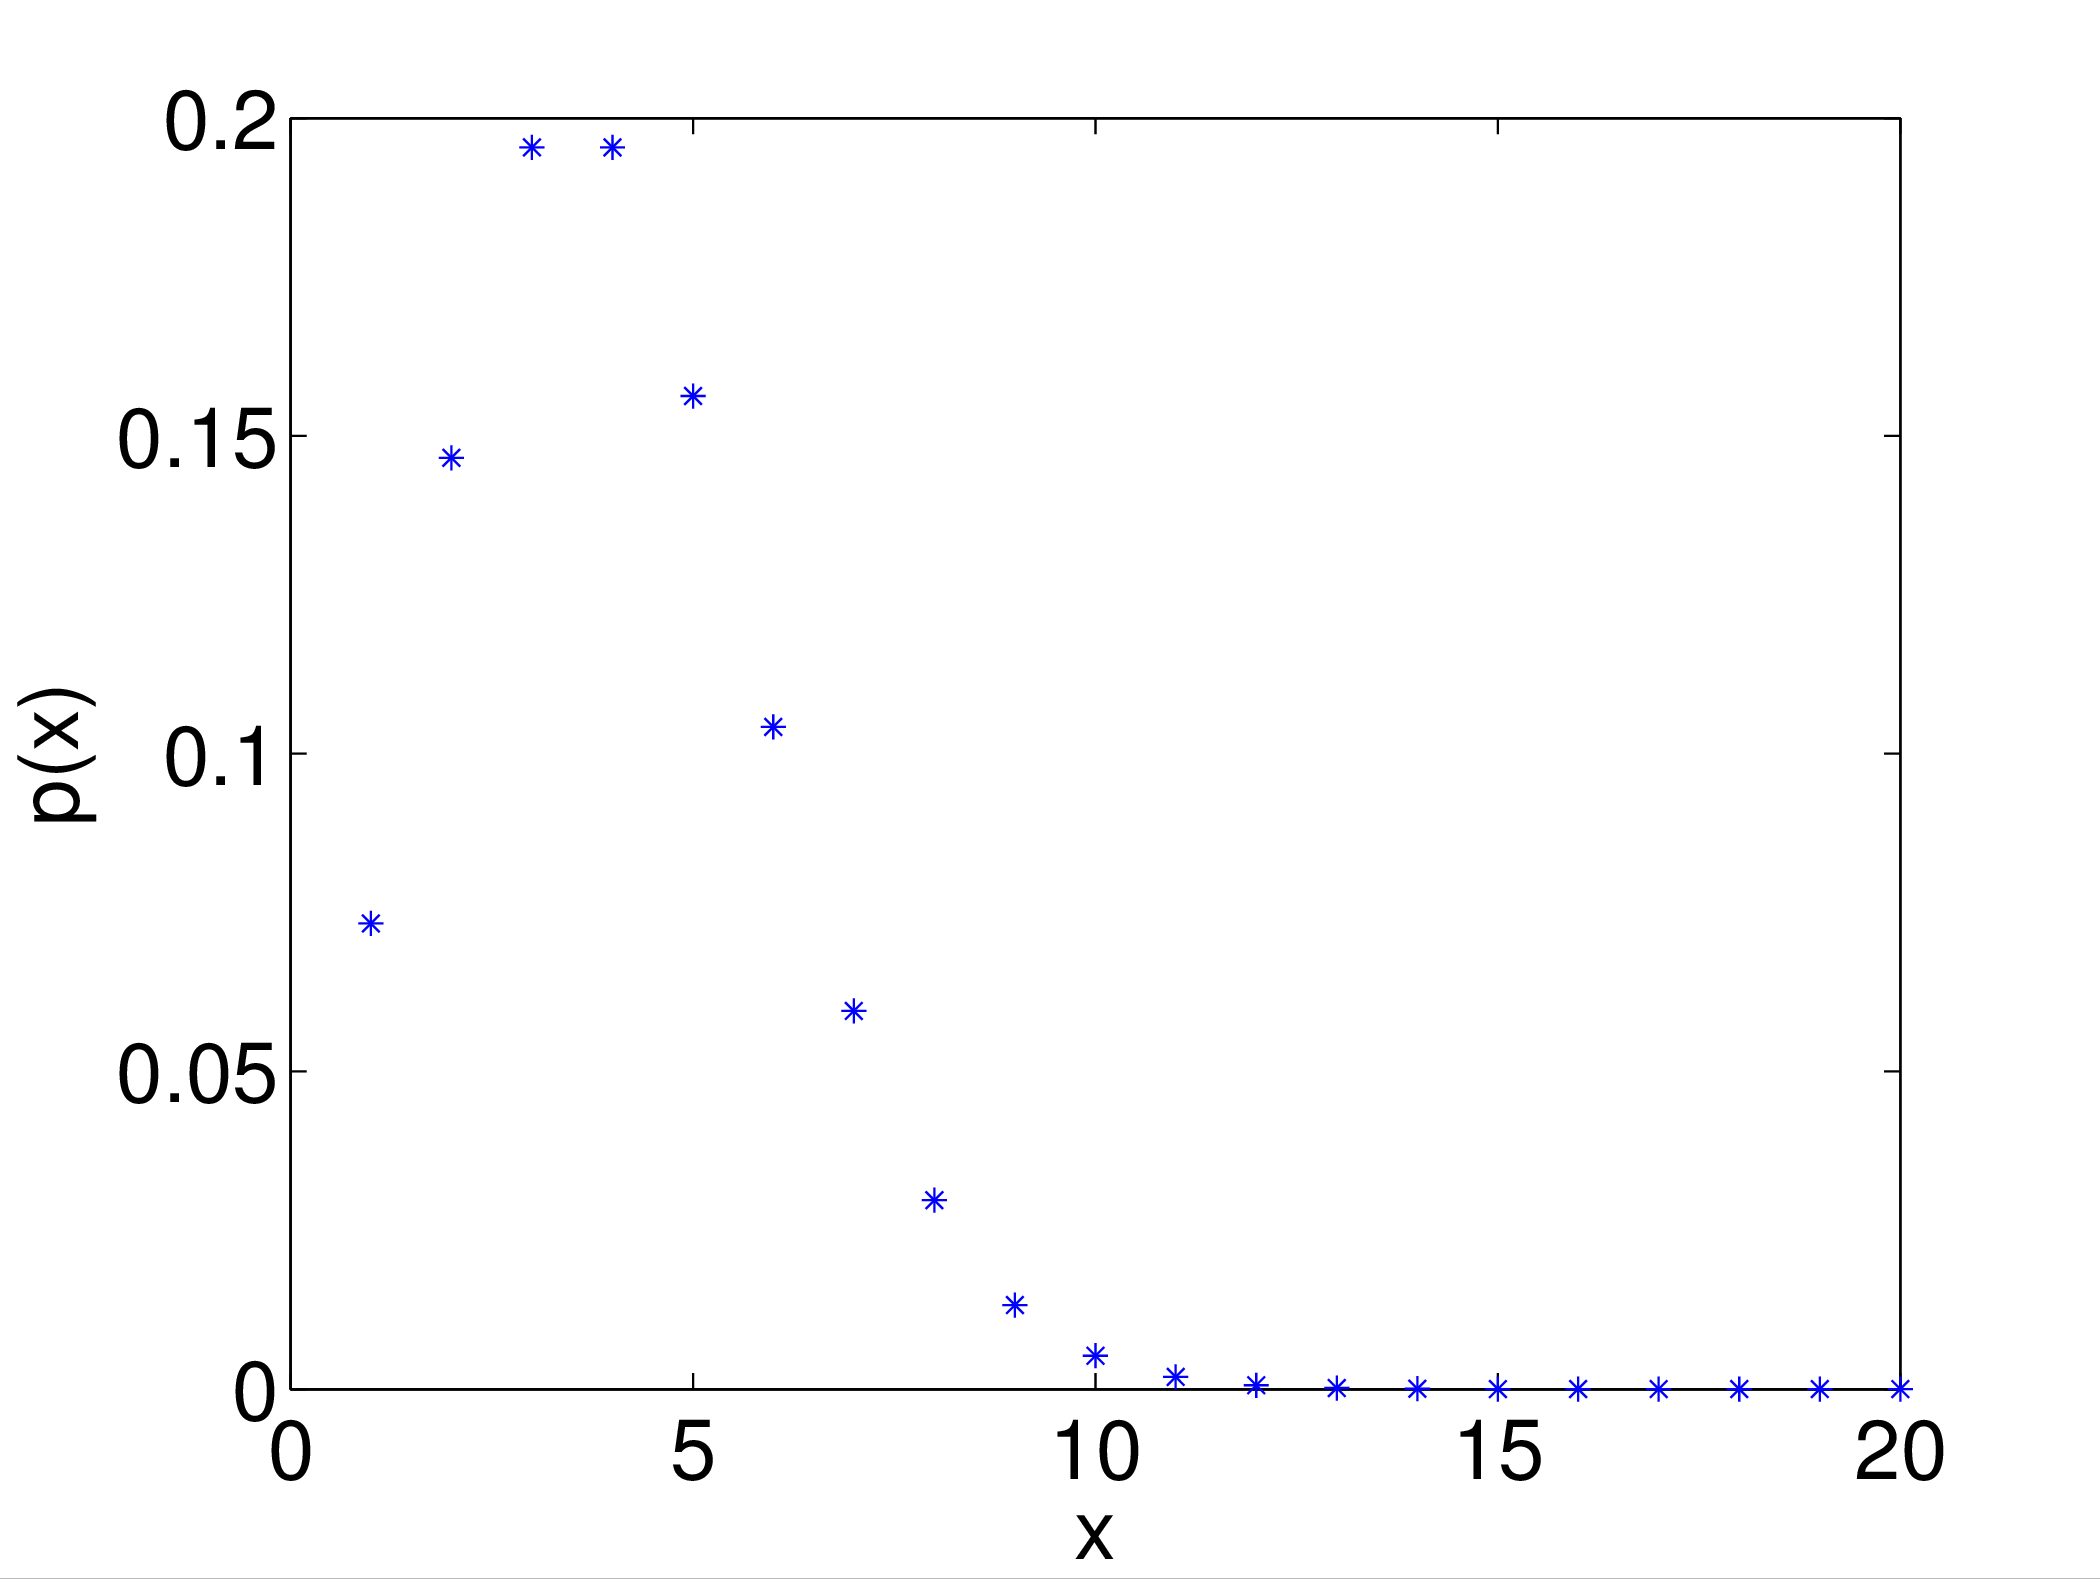
\includegraphics[scale=0.5]{poiss1} }

\end{frame}


\begin{frame}[fragile]\frametitle{An example}

\center{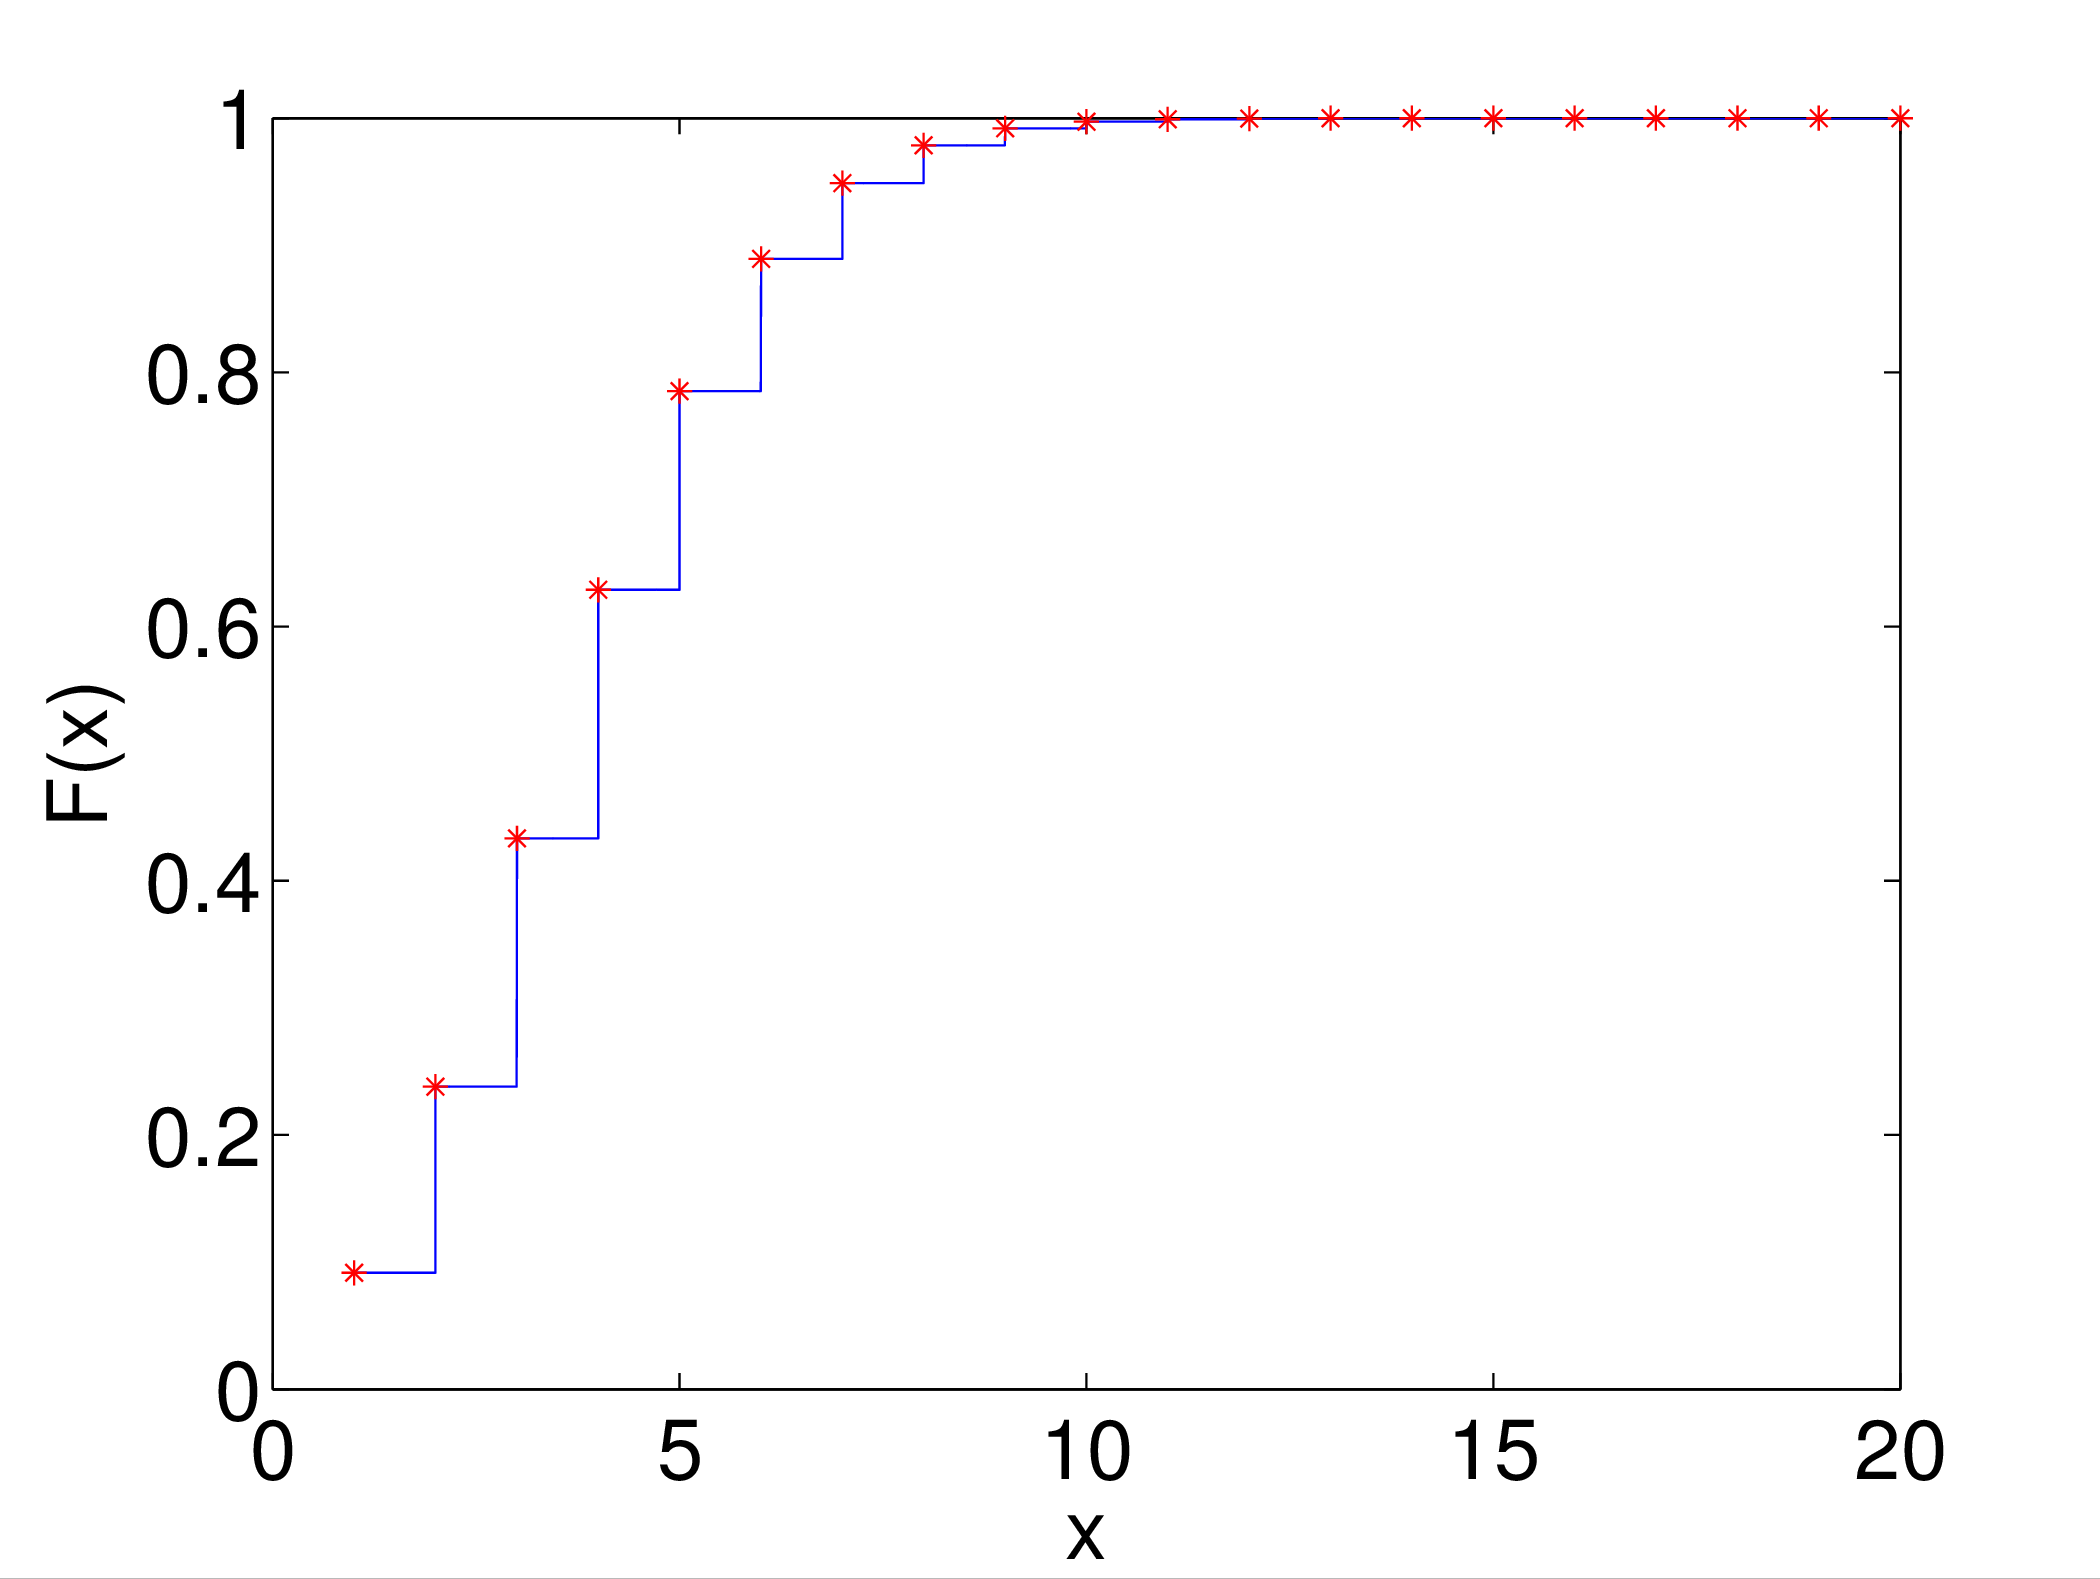
\includegraphics[scale=0.5]{poiss2} }

\end{frame}




\begin{frame}[fragile]\frametitle{Matlab code}

{\tiny
\begin{tabbing}
x= 1:20;\\
y = poisscdf(x,4);\\
i=1:.001:20;\\
$[$dum,ind$]$ = size$($i$)$;\\
vals = zeros(1,ind);\\
for \= j=1:ind \\
\>  vals(1,j) = y(floor(i(j))); \\
end \\

plot(i,vals,'-') \\
hold on \\
plot(x,y,'r*') \\
hold off;  \\

h=gca; \\
set(h,'FontSize',[20]); \\
xlabel('x'); \\
ylabel('F(x)');  \\


\end{tabbing}
}
\end{frame}



\begin{frame}[fragile]\frametitle{Pregnancy}

The pdf of $X$ is
$$p(x) = (1-p)^{x-1}p, \, \, \, \, \, \, \, x=1,2,3,...$$ 

\vspace{.1in}
Compute the cdf
$$F(x) = \sum_{i=1}^x (1-p)^{i-1}p=p\sum_{i=1}^x (1-p)^{i-1} = p
\sum_{i=0}^{x-1} (1-p)^{i}.$$
$$\sum_{i=0}^k a^i = \frac{1-a^{k+1}}{1-a}$$
which implies
$$F(x) = p\frac{1-(1-p)^x}{1-(1-p)} = 1-(1-p)^x.$$


\end{frame}



%%%%%%%%%%%%%%%%%%%%%%%%%%%%%%%%%%%%%%%%%%%%%%%%%%%%%%%%%%%%%%%%%%%%%%%%%%%%%%%%%%
\begin{frame}[fragile]\frametitle{}
\begin{center}
{\Large Expectation and variance}

\end{center}
\end{frame}




\begin{frame}[fragile]\frametitle{Expectation of a discrete rv}
\begin{defn}
Let $X$ be a discrete rv with a set of possible values $D$ and pdf
$p(x)$. The {\bf expected} or {\bf mean} value of $X$ is
$$ \mathbb E[X] = \mu_{_X} = \sum_{x \in D} x \cdot p(x).$$
\end{defn}

\end{frame}



\begin{frame}[fragile]\frametitle{Examples}

Bernoulli:

$X = \{0,1\}$ \\
$$p(x;\alpha) = \left\{\begin{array}{ll}
			1-\alpha & \mbox{if } x =0 \\
			\alpha & \mbox{if } x=1
						   .	\end{array}
						\right. $$ 	 \\ 

$$\mu_{_X} = 0 \cdot (1-\alpha) + 1 \cdot \alpha = \alpha.$$


\end{frame}



\begin{frame}[fragile]\frametitle{Pregnancy}

The pdf of $X$ is
$$p(x) = p(1-p)^{x-1}, \, \, \, \, \, \, \, x=1,2,3,...$$ 

$$\mu_{_X} = \sum_{x=1}^\infty x \cdot p(x) = \sum_{x=1}^\infty x \cdot
(1-p)^{x-1}p= \frac{1}{p}.$$ 


\end{frame}



\begin{frame}[fragile]\frametitle{Another example}

$$\mu_{_X} = 0.0491$$ 
\center{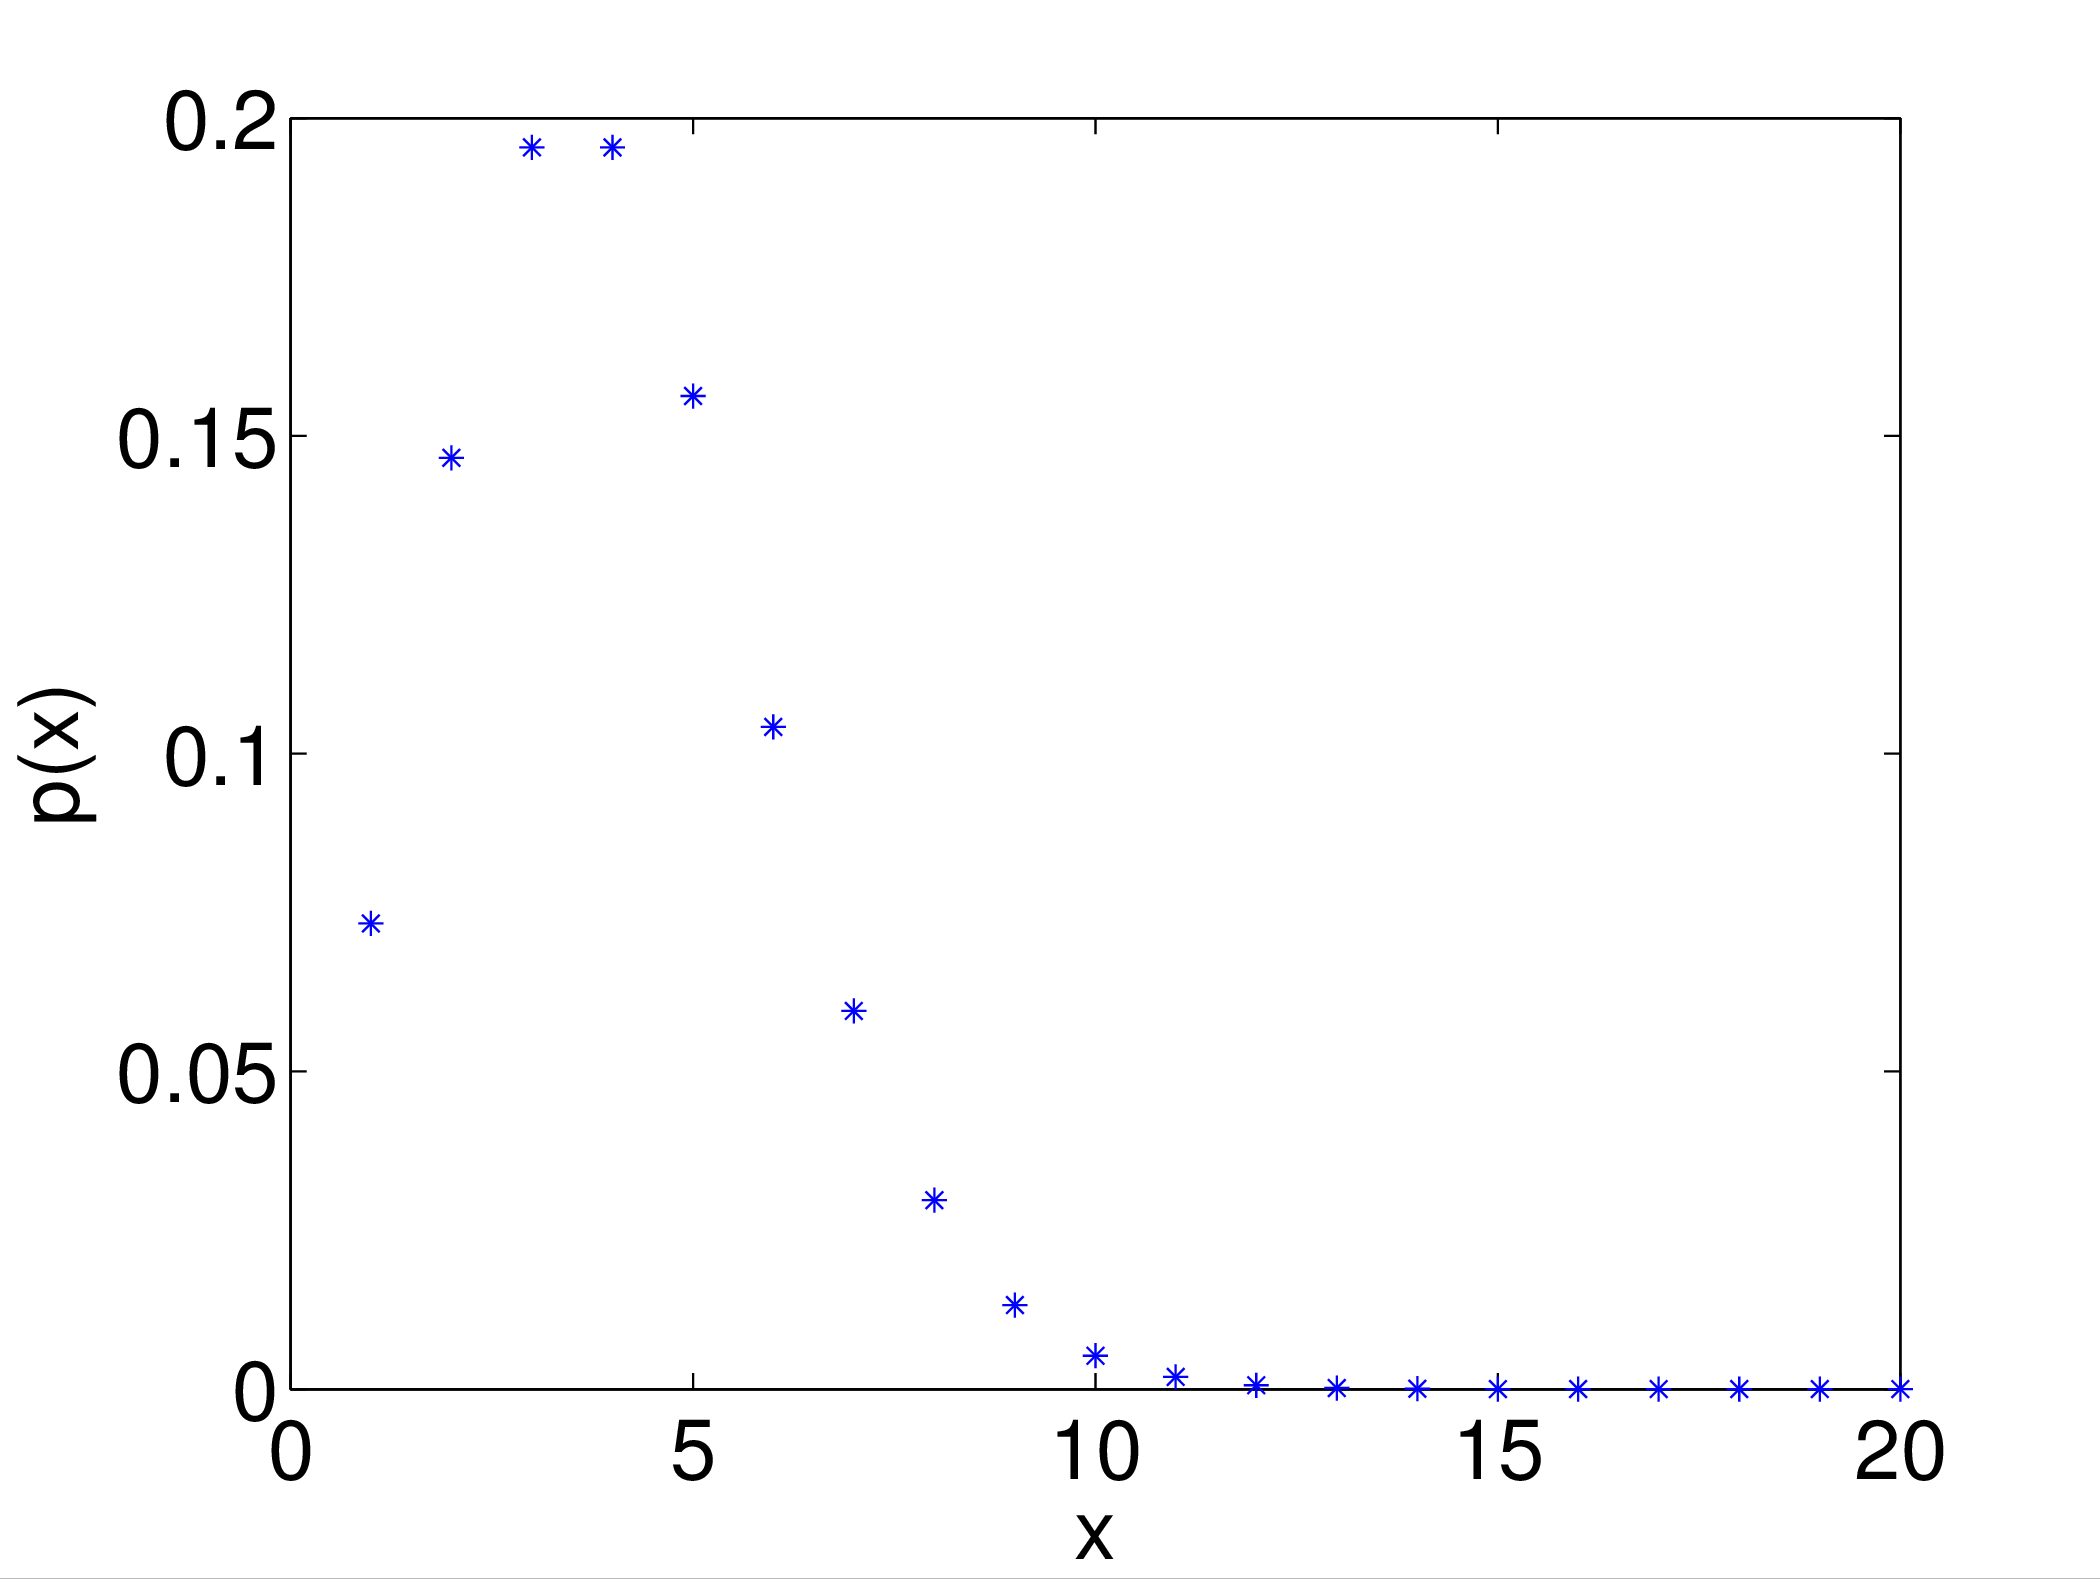
\includegraphics[scale=0.4]{poiss1} }

\end{frame}



\begin{frame}[fragile]\frametitle{Heavy tails}

The discrete rv $X$ takes values $x=1,2,3,....$ and has
pdf
$$p(x) = \frac{6}{\pi^2} \frac{1}{x^2}.$$ 
Why $\frac{6}{\pi^2}$ ?

What is the mean
$$\mu_{_X} = \frac{6}{\pi^2} \sum_{x=1}^{\infty} x \cdot \frac{1}{x^2}
= \frac{6}{\pi^2} \sum_{x=1}^\infty \frac{1}{x} = \infty.$$ 

\end{frame}



\begin{frame}[fragile]\frametitle{Heavy tail}

\center{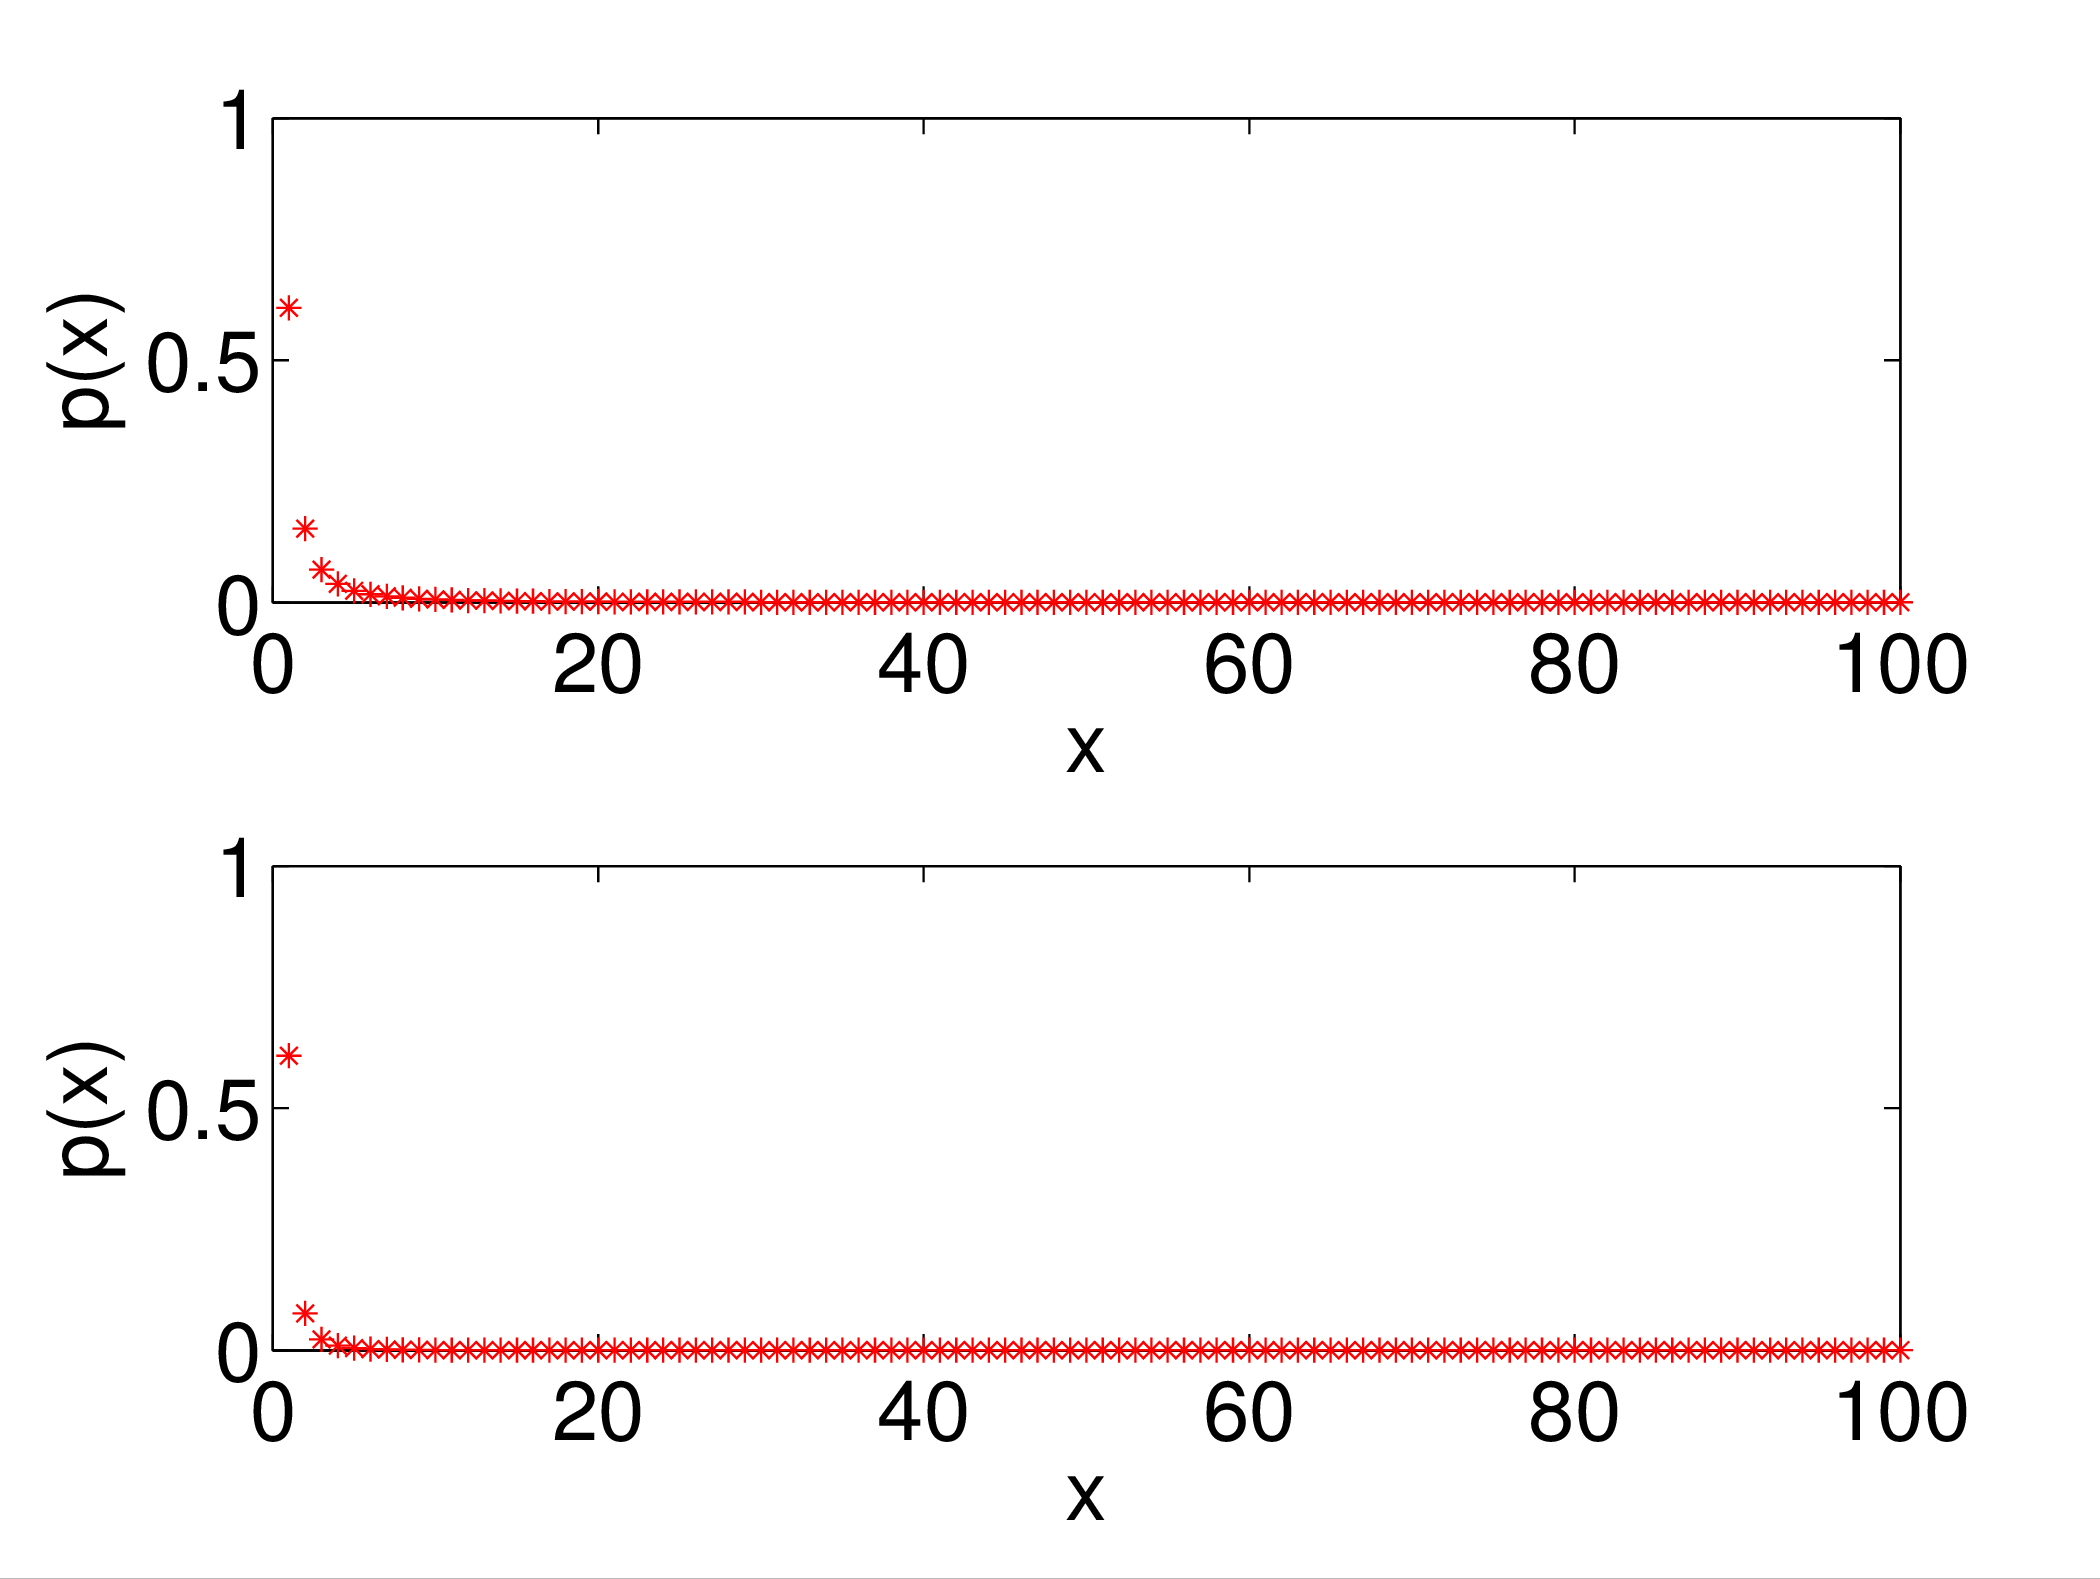
\includegraphics[scale=0.4]{ht1} }

\end{frame}


\begin{frame}[fragile]\frametitle{Heavy tail: semilog}

\center{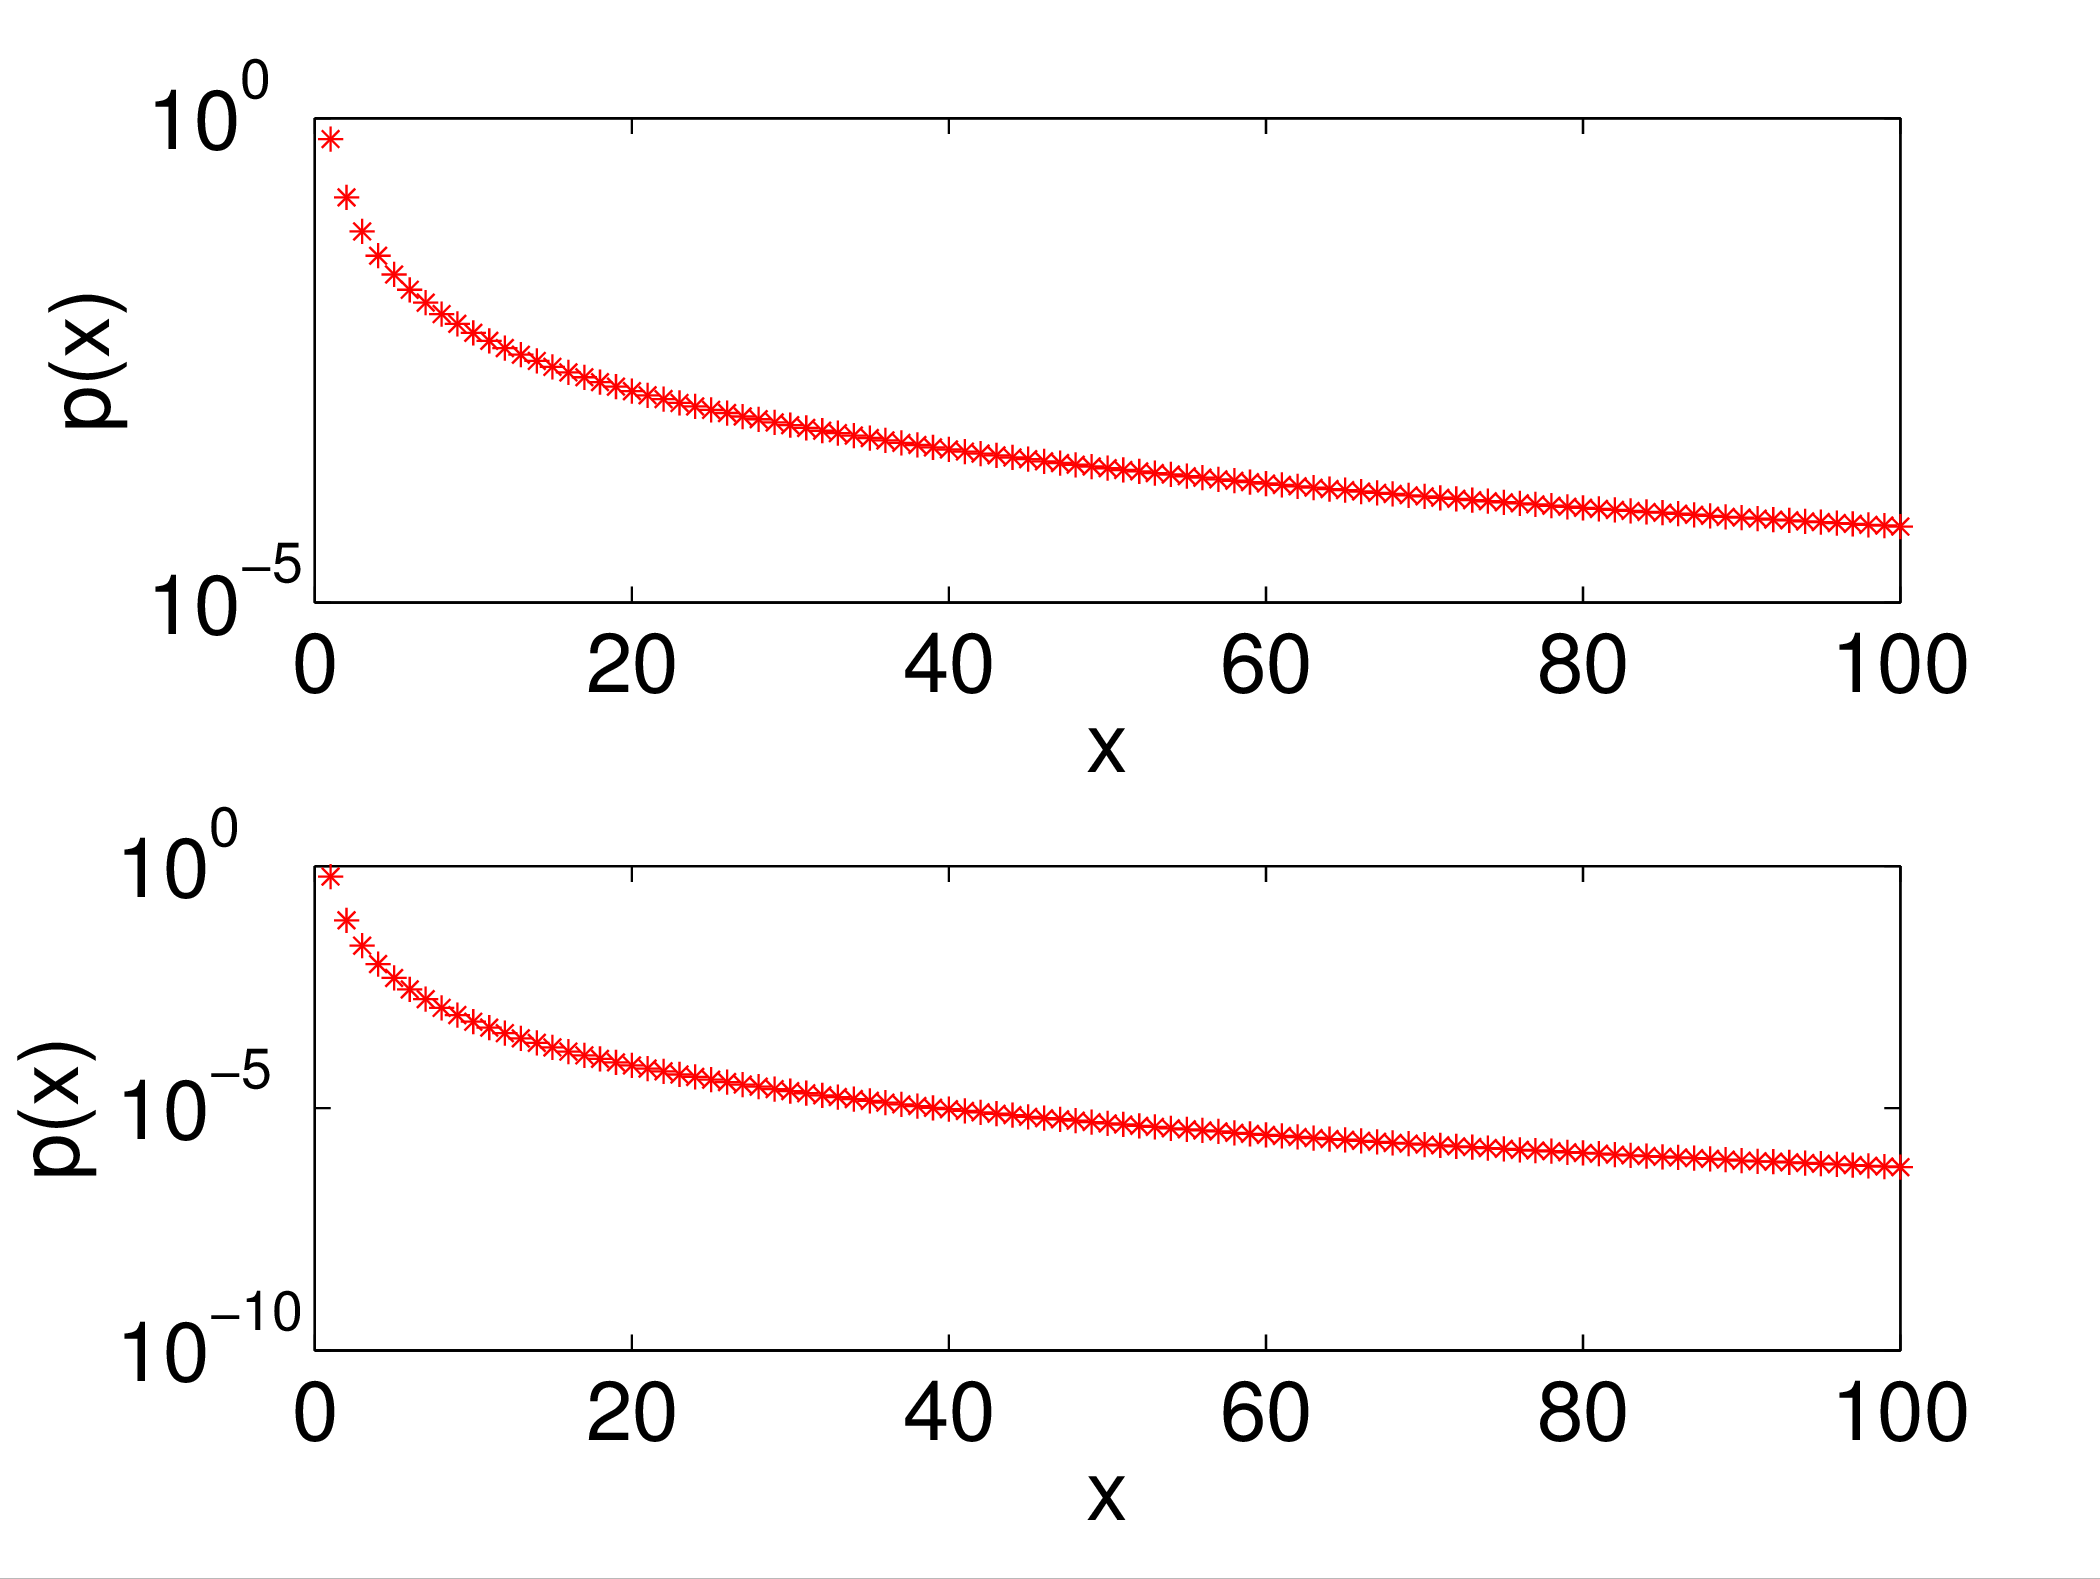
\includegraphics[scale=0.4]{ht2} }

\end{frame}


\begin{frame}[fragile]\frametitle{Matlab code: page 1}

{\tiny

\begin{lstlisting}
figure(1)\\ 
x= 1:100; \\
y = (6/pi\^{}2)*(1./x.\^{}2);\\
subplot(2,1,1); \\
plot(x,y,'r*');\\
h=gca; \\
set(h,'FontSize',[20]); \\
xlabel('x'); \\
ylabel('p(x)'); \\

y = (6/pi\^{}2)*(1./x.\^{}3); \\
subplot(2,1,2); \\
plot(x,y,'r*'); \\
h=gca; \\
set(h,'FontSize',[20]);\\
xlabel('x');\\
ylabel('p(x)');\\
\end{lstlisting}
}

\end{frame}


\begin{frame}[fragile]\frametitle{Matlab code: page 2}

{\tiny

\begin{lstlisting}
figure(2)\\ 
x= 1:100; \\
y = (6/pi\^{}2)*(1./x.\^{}2);\\
subplot(2,1,1); \\
semilogy(x,y,'r*'); \\
h=gca;\\
set(h,'FontSize',[20]); \\
xlabel('x'); \\ 
ylabel('p(x)'); \\
 
y = (6/pi\^{}2)*(1./x.\^{}3); \\
subplot(2,1,2); \\
semilogy(x,y,'r*');\\
h=gca; \\
set(h,'FontSize',[20]);\\
xlabel('x'); \\
ylabel('p(x)'); \\
\end{lstlisting}
}
\end{frame}



\begin{frame}[fragile]\frametitle{Expectation of a function of a discrete rv}

\begin{prop}
Let $X$ be a discrete rv with a set of possible values $D$ and pdf
$p(x)$. The expectation of a function $h(X)$ is
$$ \mathbb E[h(X)] = \sum_{x \in D} h(x) \cdot p(x).$$
\end{prop}

\end{frame}


\begin{frame}[fragile]\frametitle{Linearity of expectation}

\begin{prop}
\begin{eqnarray*}
\mathbb E[aX+b] &=& \sum_{x \in D} (ax+b) \cdot p(x), \\ 
 & = & \sum_{x \in D} ax \cdot p(x)+ \sum_{x \in D} b \cdot p(x),\\  
  & = & a \sum_{x \in D} x \cdot p(x)+ b \sum_{x \in D} p(x),\\ 
  & = & a \mathbb E[X]+ b ,\\ 
& = & a \mu_{_X}+ b.
\end{eqnarray*}
\end{prop}

\end{frame}



\begin{frame}[fragile]\frametitle{Variance of a discrete rv}
\begin{defn}
Let $X$ be a discrete rv with a set of possible values $D$ and pdf
$p(x)$. The {\bf variance} of $X$ is
\begin{eqnarray*}
\mathbb V[X] &=& \sigma^2_{_X}\\ 
& =& \mathbb E[(X-\mu_{_X})^2]\\ 
&=& \sum_{x \in D} (x-\mu_{_X})^2 \cdot p(x). 
\end{eqnarray*}

The {\bf standard deviation} $\sigma_{_X} = \sqrt{\sigma^2_{_X}}$.
\end{defn}

\end{frame}



\begin{frame}[fragile]\frametitle{Examples}

Bernoulli:

$X = \{0,1\}$ \\
$$p(x;\alpha) = \left\{\begin{array}{ll}
			1-\alpha & \mbox{if } x =0 \\
			\alpha & \mbox{if } x=1
						   .	\end{array}
						\right. $$ 	 \\ 

\begin{eqnarray*}
\sigma^2_{_X}& =& (0-\alpha)^2 \cdot (1-\alpha) + (1-\alpha)^2 \cdot
\alpha, \\ 
 & = & \alpha^2-\alpha^3 + (1- 2 \alpha+ \alpha^2) \alpha \\ 
& = & \alpha^2 - \alpha^3 + \alpha - 2 \alpha^2 + \alpha^3 \\ 
& = & \alpha - \alpha^2  \\ 
& = & \alpha(1 - \alpha)  \\ 
\end{eqnarray*} 


\end{frame}




\begin{frame}[fragile]\frametitle{Properties of variance}

\begin{eqnarray*}
\mathbb V[X] &=& \mathbb E[(X-\mu_{_X})^2]\\ 
& =& \mathbb E[(X^2 -2 X \mu_{_X} + \mu^2_{_X})],\\ 
&=& \mathbb E[X^2]- 2 \mathbb E[X] \mu_{_X} + \mu^2_{_X}, \\ 
&=& \mathbb E[X^2]- 2 \mu^2_{_X} + \mu^2_{_X}, \\ 
&=& \mathbb E[X^2]- \mu^2_{_X}, \\ 
&=& \mathbb E[X^2]- (\mathbb E[X])^2.
\end{eqnarray*}


\end{frame}



\begin{frame}[fragile]\frametitle{Variance of a function of a discrete rv}

\begin{prop}
Let $X$ be a discrete rv with a set of possible values $D$ and pdf
$p(x)$. The variance of a function $h(X)$ is
$$\mathbb V[h(X)] = \mathbb E[(h(X)- \mathbb E[h(x)])^2].$$
\end{prop}

\end{frame}


\begin{frame}[fragile]\frametitle{More properties of variance}

\begin{eqnarray*}
\mathbb V[aX+b] &=& \mathbb E[(aX+b)^2]- (\mathbb E[aX+b])^2. \\ 
          &=& \mathbb E[a^2 X^2+ 2ab X +  b^2] - (a \mu+b)^2. \\ 
          &=& \mathbb E[a^2 X^2] + \mathbb E[2ab X] +  b^2 - a^2 \mu^2 - b^2 + 2 \mu ab. \\ 
          &=& a^2 \mathbb E[X^2] + 2 ab \mathbb E[X] + b^2 - a^2 \mu^2 - b^2 + 2 \mu ab. \\ 
          &=& a^2 \mathbb E[X^2] + 2 ab \mu + b^2 - a^2 \mu^2 - b^2 + 2 \mu ab. \\ 
          &=& a^2 \mathbb E[X^2] -a^2 \mu^2, \\ 
          & = & a^2 \mathbb V[X].
\end{eqnarray*}


\end{frame}


%%%%%%%%%%%%%%%%%%%%%%%%%%%%%%%%%%%%%%%%%%%%%%%%%%%%%%%%%%%%%%%%%%%%%%%%%%%%%%%%%%
\begin{frame}[fragile]\frametitle{}
\begin{center}
{\Large Discrete distributions}

\end{center}
\end{frame}


\begin{frame}[fragile]\frametitle{Two ways}

There are at least two ways to think about distributions: 
\begin{enumerate} 

\item the distribution function $p(x)$ 

\item an experiment that generates the distribution. 

\end{enumerate}

It is good to have an idea of both because one or the other
may be more useful at times.

\end{frame}

%%%%%%%%%%%%%%%%%%%%%%%%%%%%%%%%%%%%%%%%%%%%%%%%%%%%%%%%%%%%%%%%%%%%%%%%%%%%%%%%%%
\begin{frame}[fragile]\frametitle{}
\begin{center}
{\Large Bernoulli}

\end{center}
\end{frame}



\begin{frame}[fragile]\frametitle{Bernoulli}

$X = \{0,1\}$ \\
$$p(x;p) = \left\{\begin{array}{ll}
			1-p & \mbox{if } x =0 \\
			p & \mbox{if } x=1
						   .	\end{array}
						\right. $$ 	 \\ 

\vspace{.1in}

What is the corresponding experiment ?  \\
Flip a coin once with $\pr(H) = p$. This is a Bernoulli trial.


\end{frame}


%%%%%%%%%%%%%%%%%%%%%%%%%%%%%%%%%%%%%%%%%%%%%%%%%%%%%%%%%%%%%%%%%%%%%%%%%%%%%%%%%%
\begin{frame}[fragile]\frametitle{}
\begin{center}
{\Large Binomial}

\end{center}
\end{frame}


\begin{frame}[fragile]\frametitle{Binomial}

The experiment: run the Bernoulli trial $n$ times with each trial
independent of the other and count the
number of $1$'s. This count is the random variable. \\ 

So the possible values of the rv $X$ are $0,1,2,...,n$. \\ 

Say $n =3$, the outcomes are  
$$000,001,010,011,100,101,110,111$$
this corresponds to $X$ taking
$$0,1,1,2,1,2,2,3.$$  \\

There are two parameters for this experiment: $n$ the number of trials
and $p$ the probability of a $1$ for each trial. \\ 

What is the pdf ?

\end{frame}


\begin{frame}[fragile]\frametitle{Binomial pdf}

\begin{thm}
The binomial probability distribution function is
$$\pr(X=x) = \mbox{bin}(x;n,p) = \binom{n}{x} p^x (1-p)^{n-x} \, \, \, \, \, x=0,1,...,n.$$ 
\end{thm}

$$\pr(\mbox{getting $x$ 1's}) = p^x (1-p)^{n-x}.$$ 
$$\{\mbox{number of ways of getting $x$ 1's}\} = \binom{n}{x}.$$ \\ 

\alert{\url{http://www.stat.berkeley.edu/~stark/Java/Html/BinHist.htm}}


\end{frame}


\begin{frame}[fragile]\frametitle{Sampling with replacement}

An urn full of red and yellow m\&ms are given to STA 113 students. 

\center{
\includegraphics[scale=0.25]{mm3} }


\end{frame}



\begin{frame}[fragile]\frametitle{Sampling with replacement}

The students are told that there are $500$ m\&ms in the urn
and $200$ are red. \\ 
Every minute they are allowed to randomly remove one m\&m from the urn, record
the color, and return the m\&m to urn. \\  \vspace{.1in}

This procedure is sampling with replacement and the distribution of the
number of red m\&ms drawn after $500$ minutes is a binomial
distribution with $n=500$ and $p=\frac{200}{500} = \frac{2}{5}.$


\end{frame}


\begin{frame}[fragile]\frametitle{The binomial pdf}

Fix $n=4$ and vary $p$.

\end{frame}



\begin{frame}[fragile]\frametitle{The binomial pdf}

\center{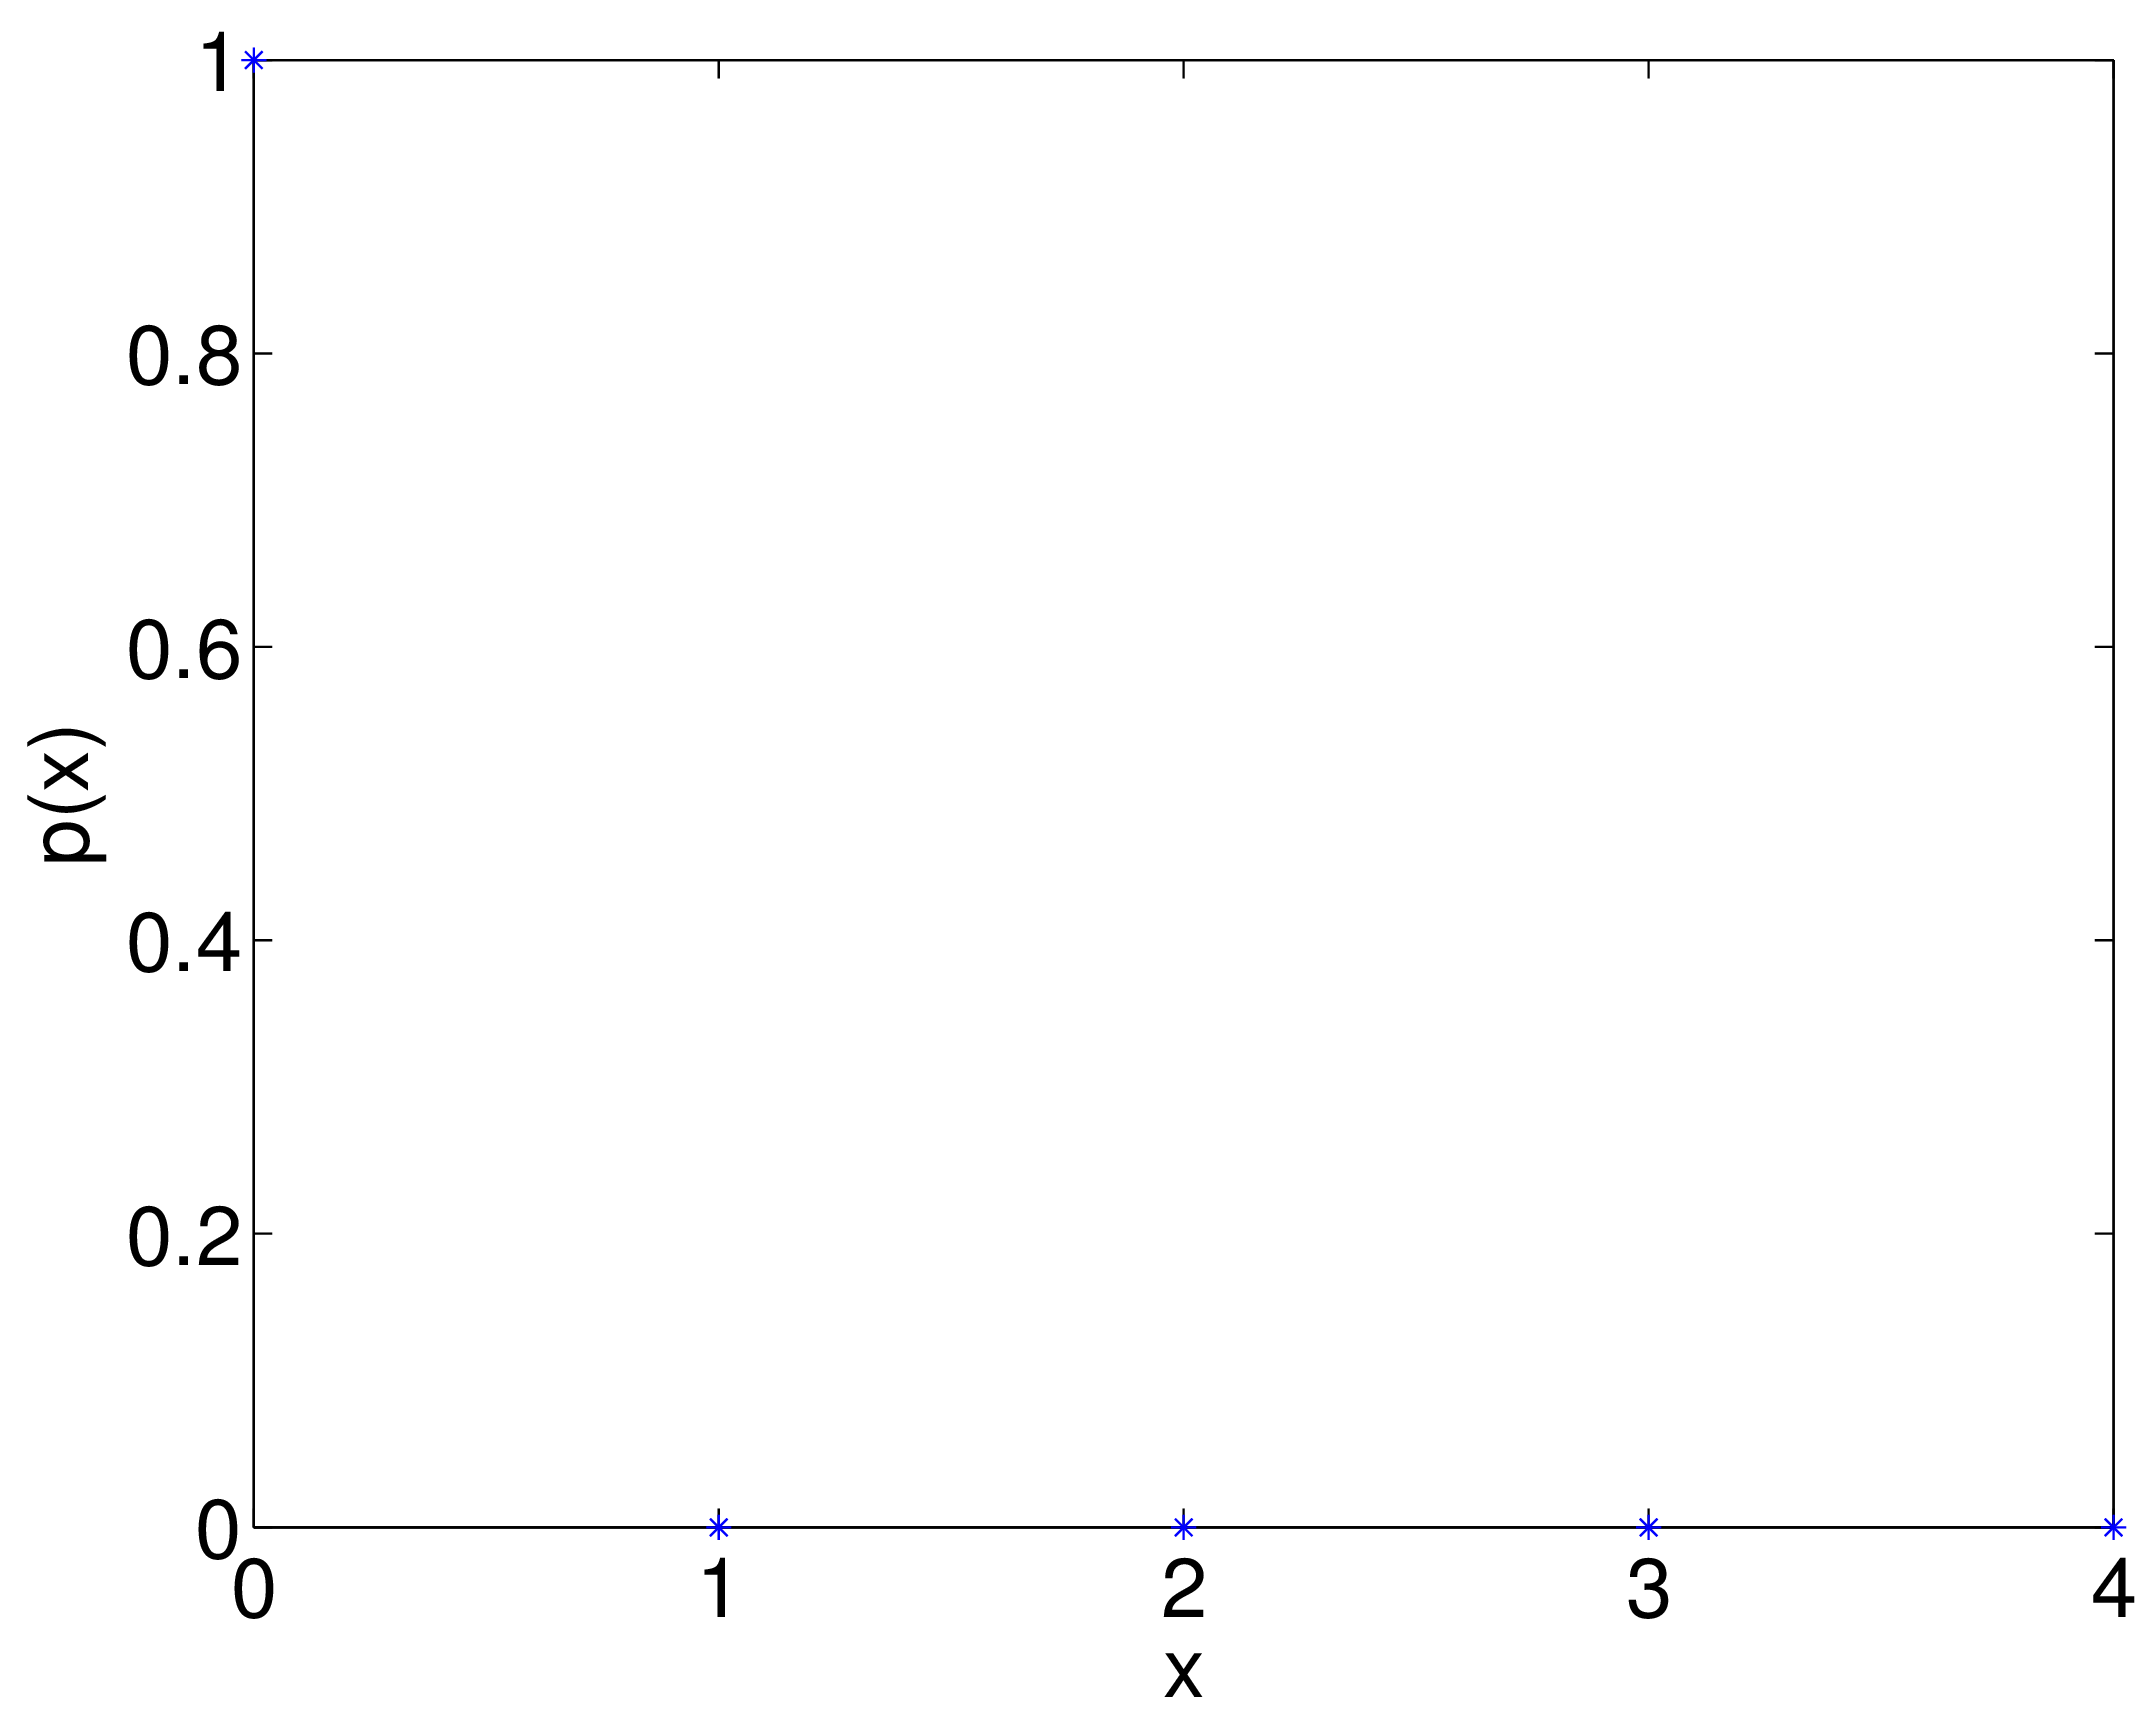
\includegraphics[scale=0.5]{bin41} }

\end{frame}



\begin{frame}[fragile]\frametitle{The binomial pdf}

\center{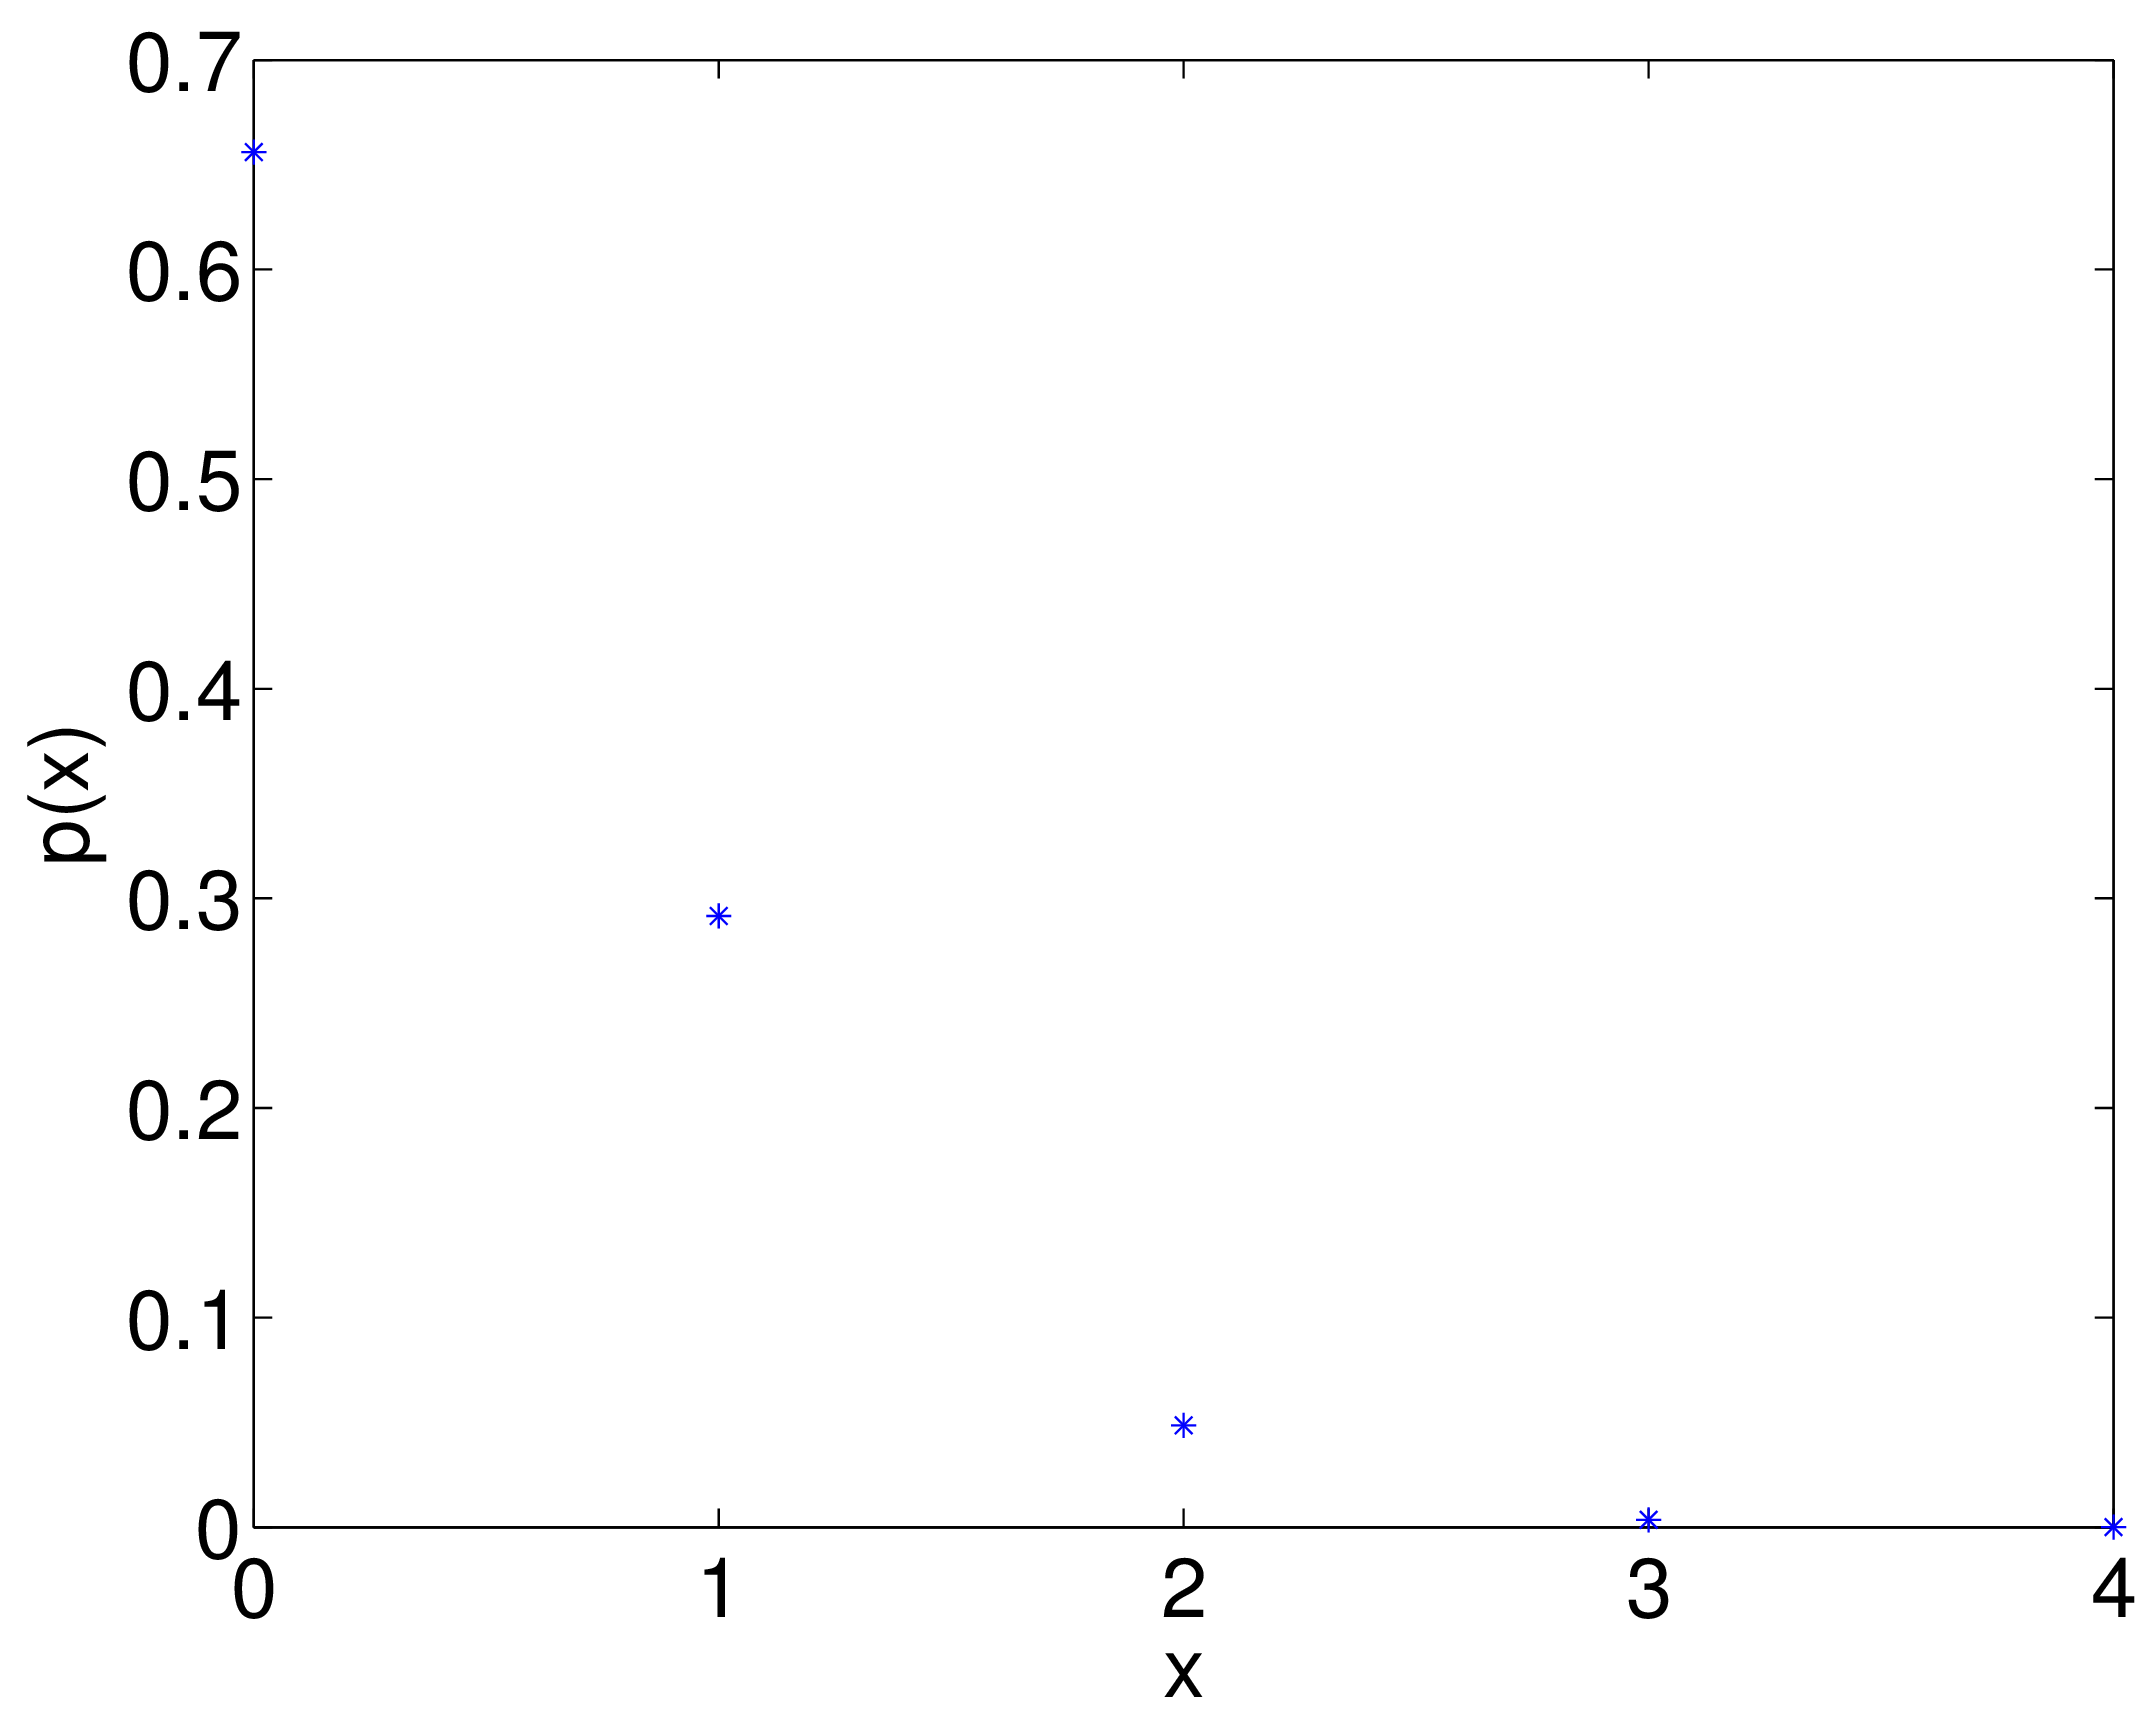
\includegraphics[scale=0.5]{bin42} }

\end{frame}

\begin{frame}[fragile]\frametitle{The binomial pdf}

\center{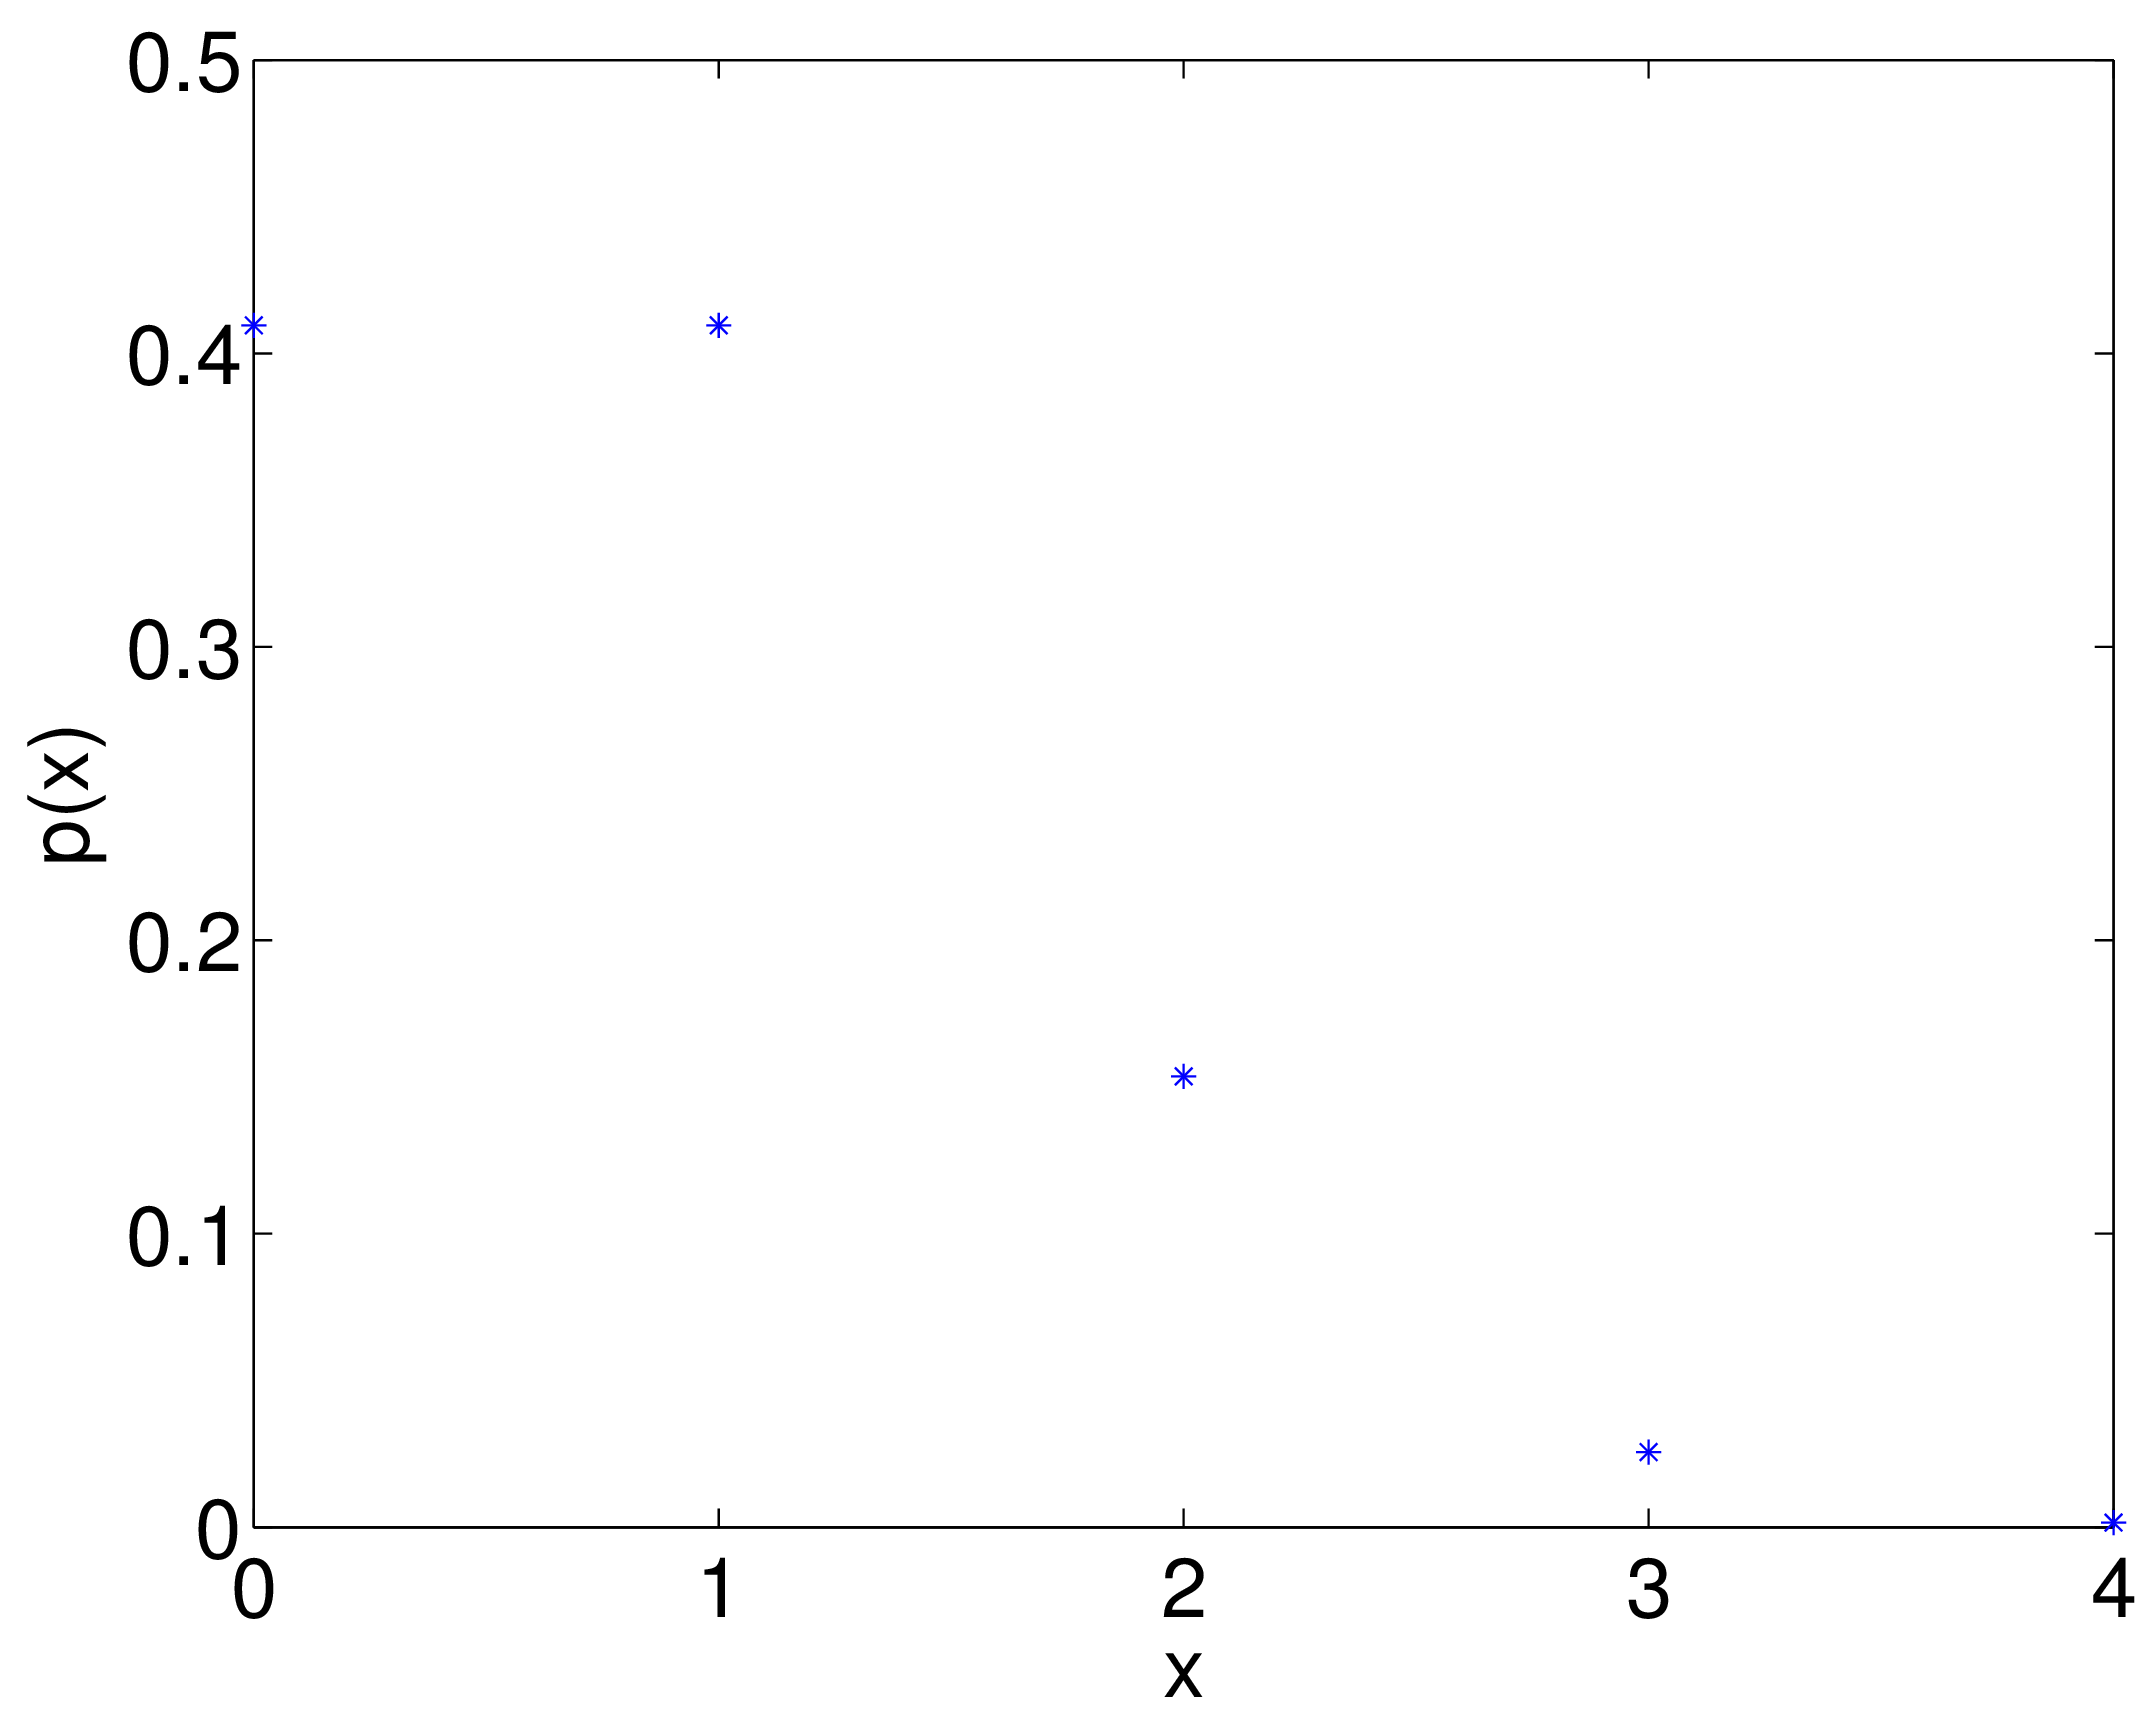
\includegraphics[scale=0.5]{bin43} }

\end{frame}

\begin{frame}[fragile]\frametitle{The binomial pdf}

\center{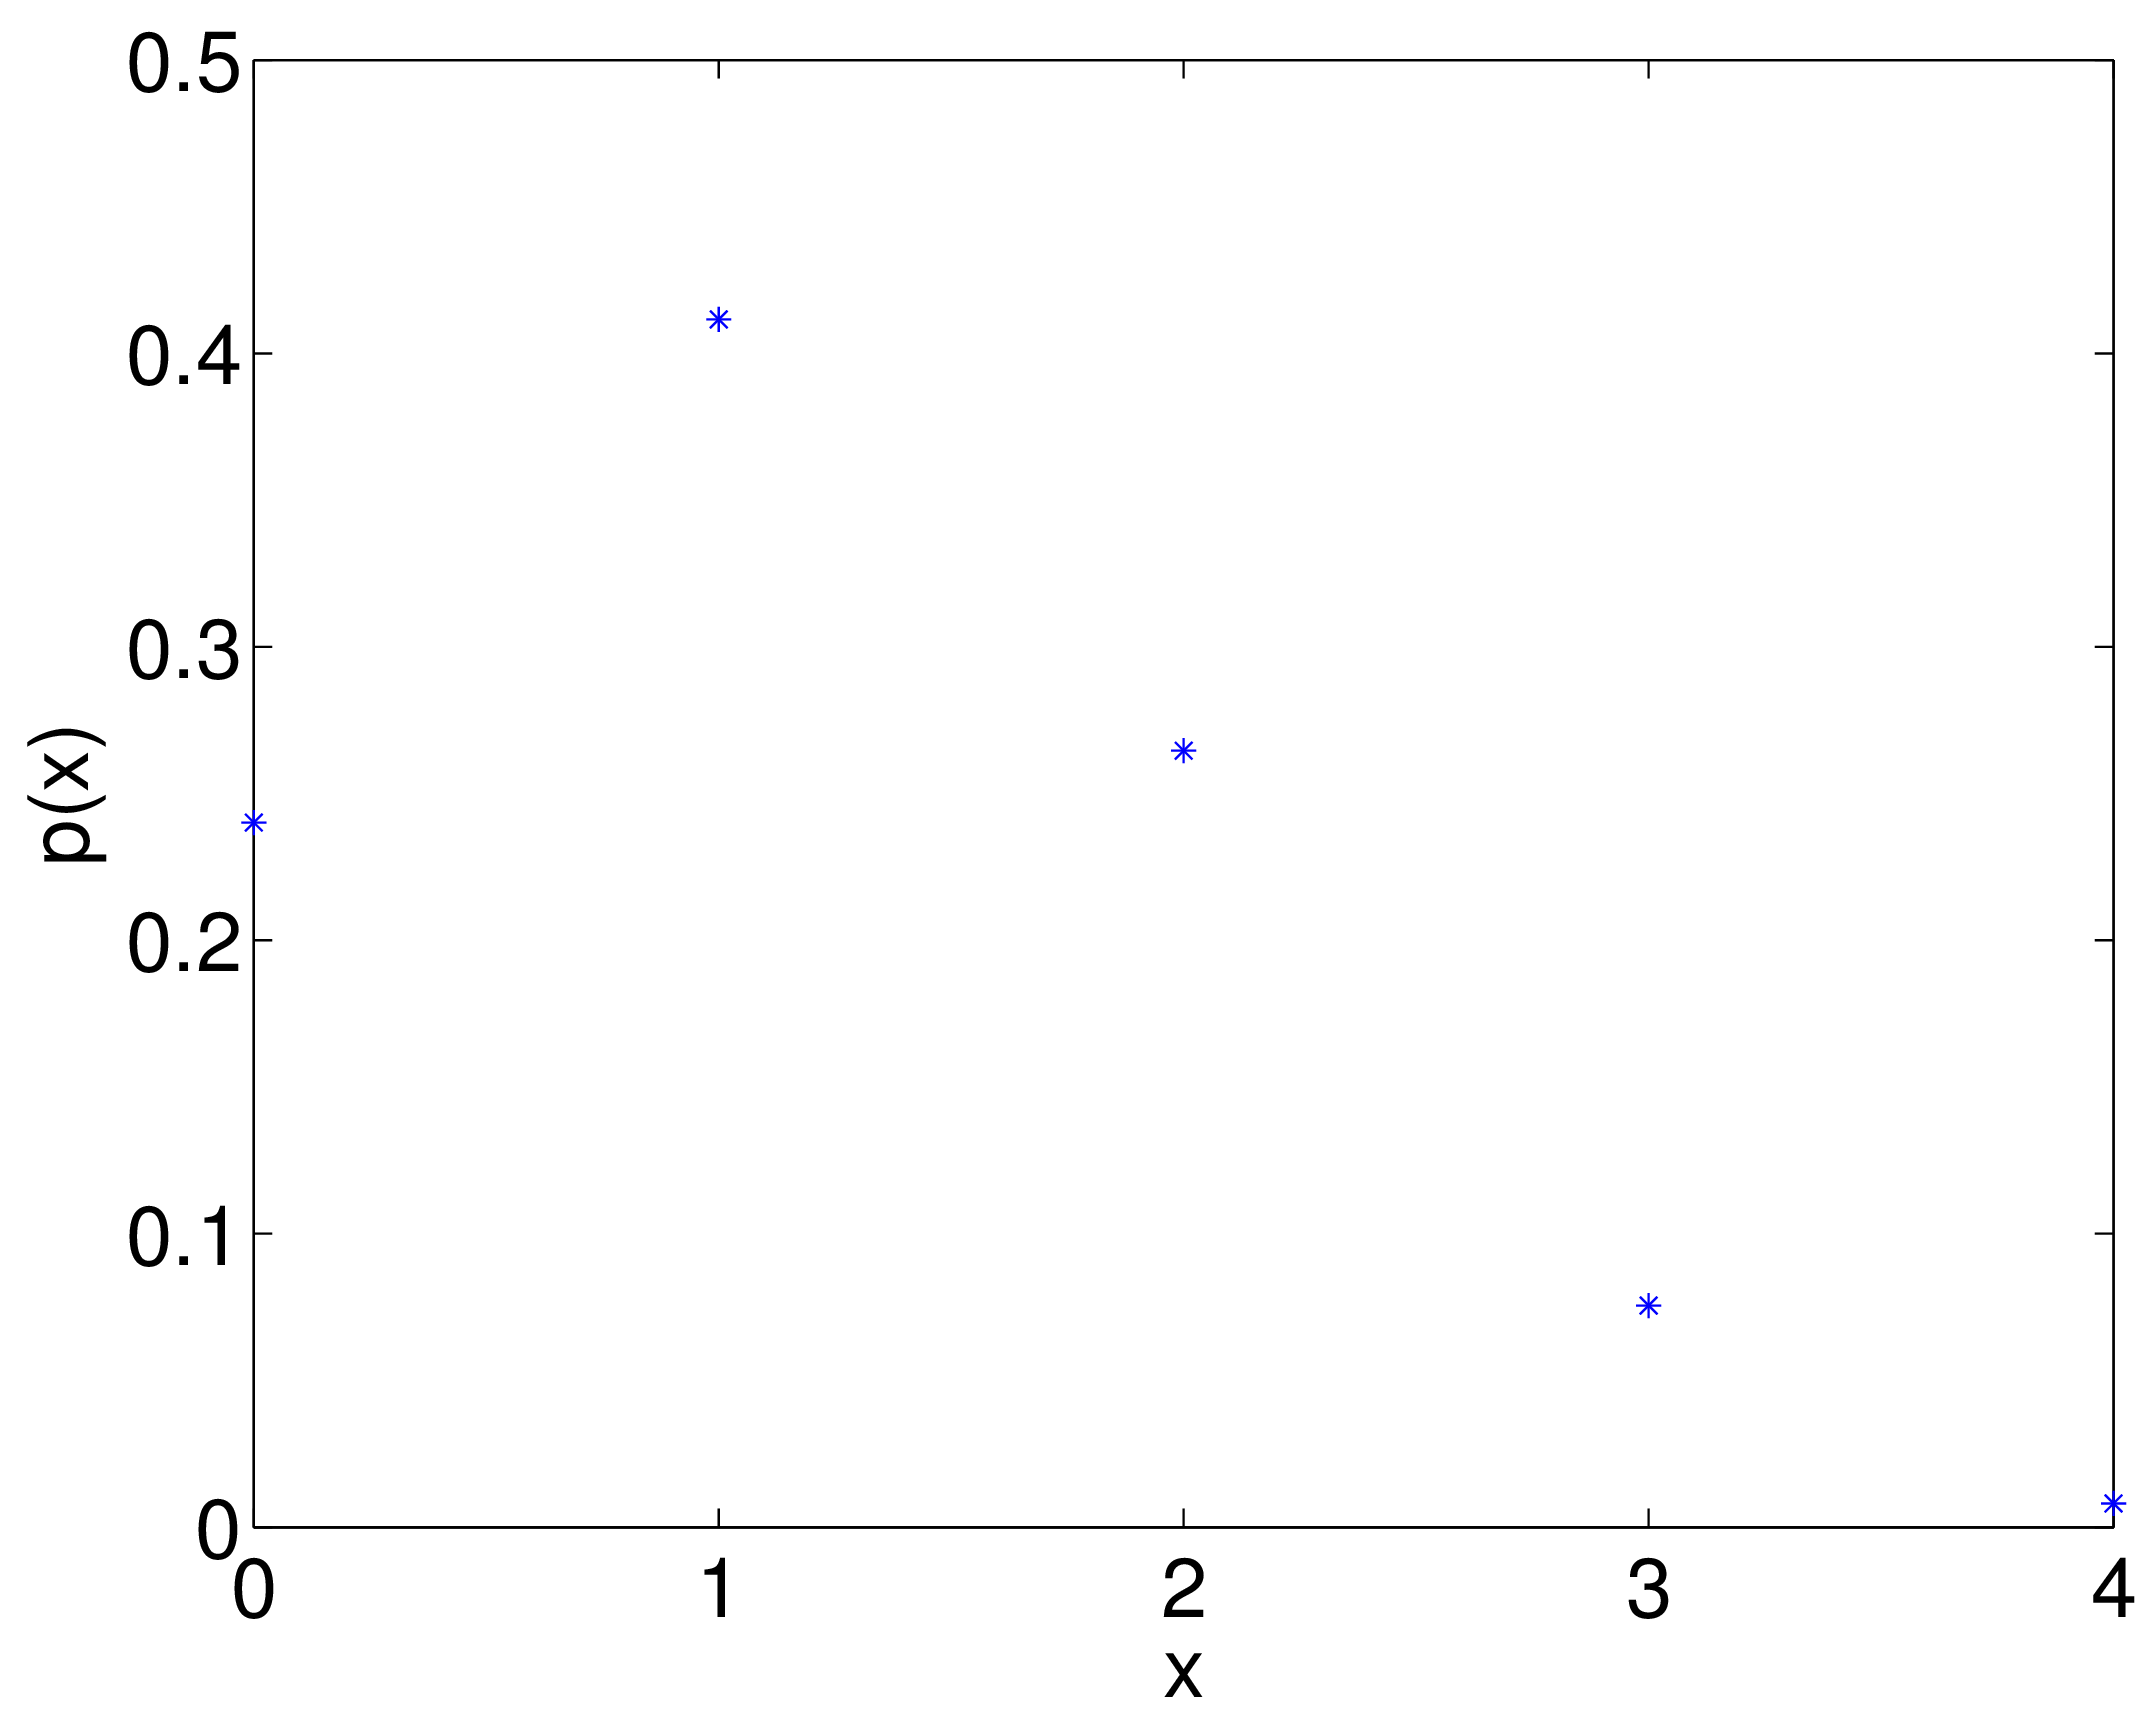
\includegraphics[scale=0.5]{bin44} }

\end{frame}

\begin{frame}[fragile]\frametitle{The binomial pdf}

\center{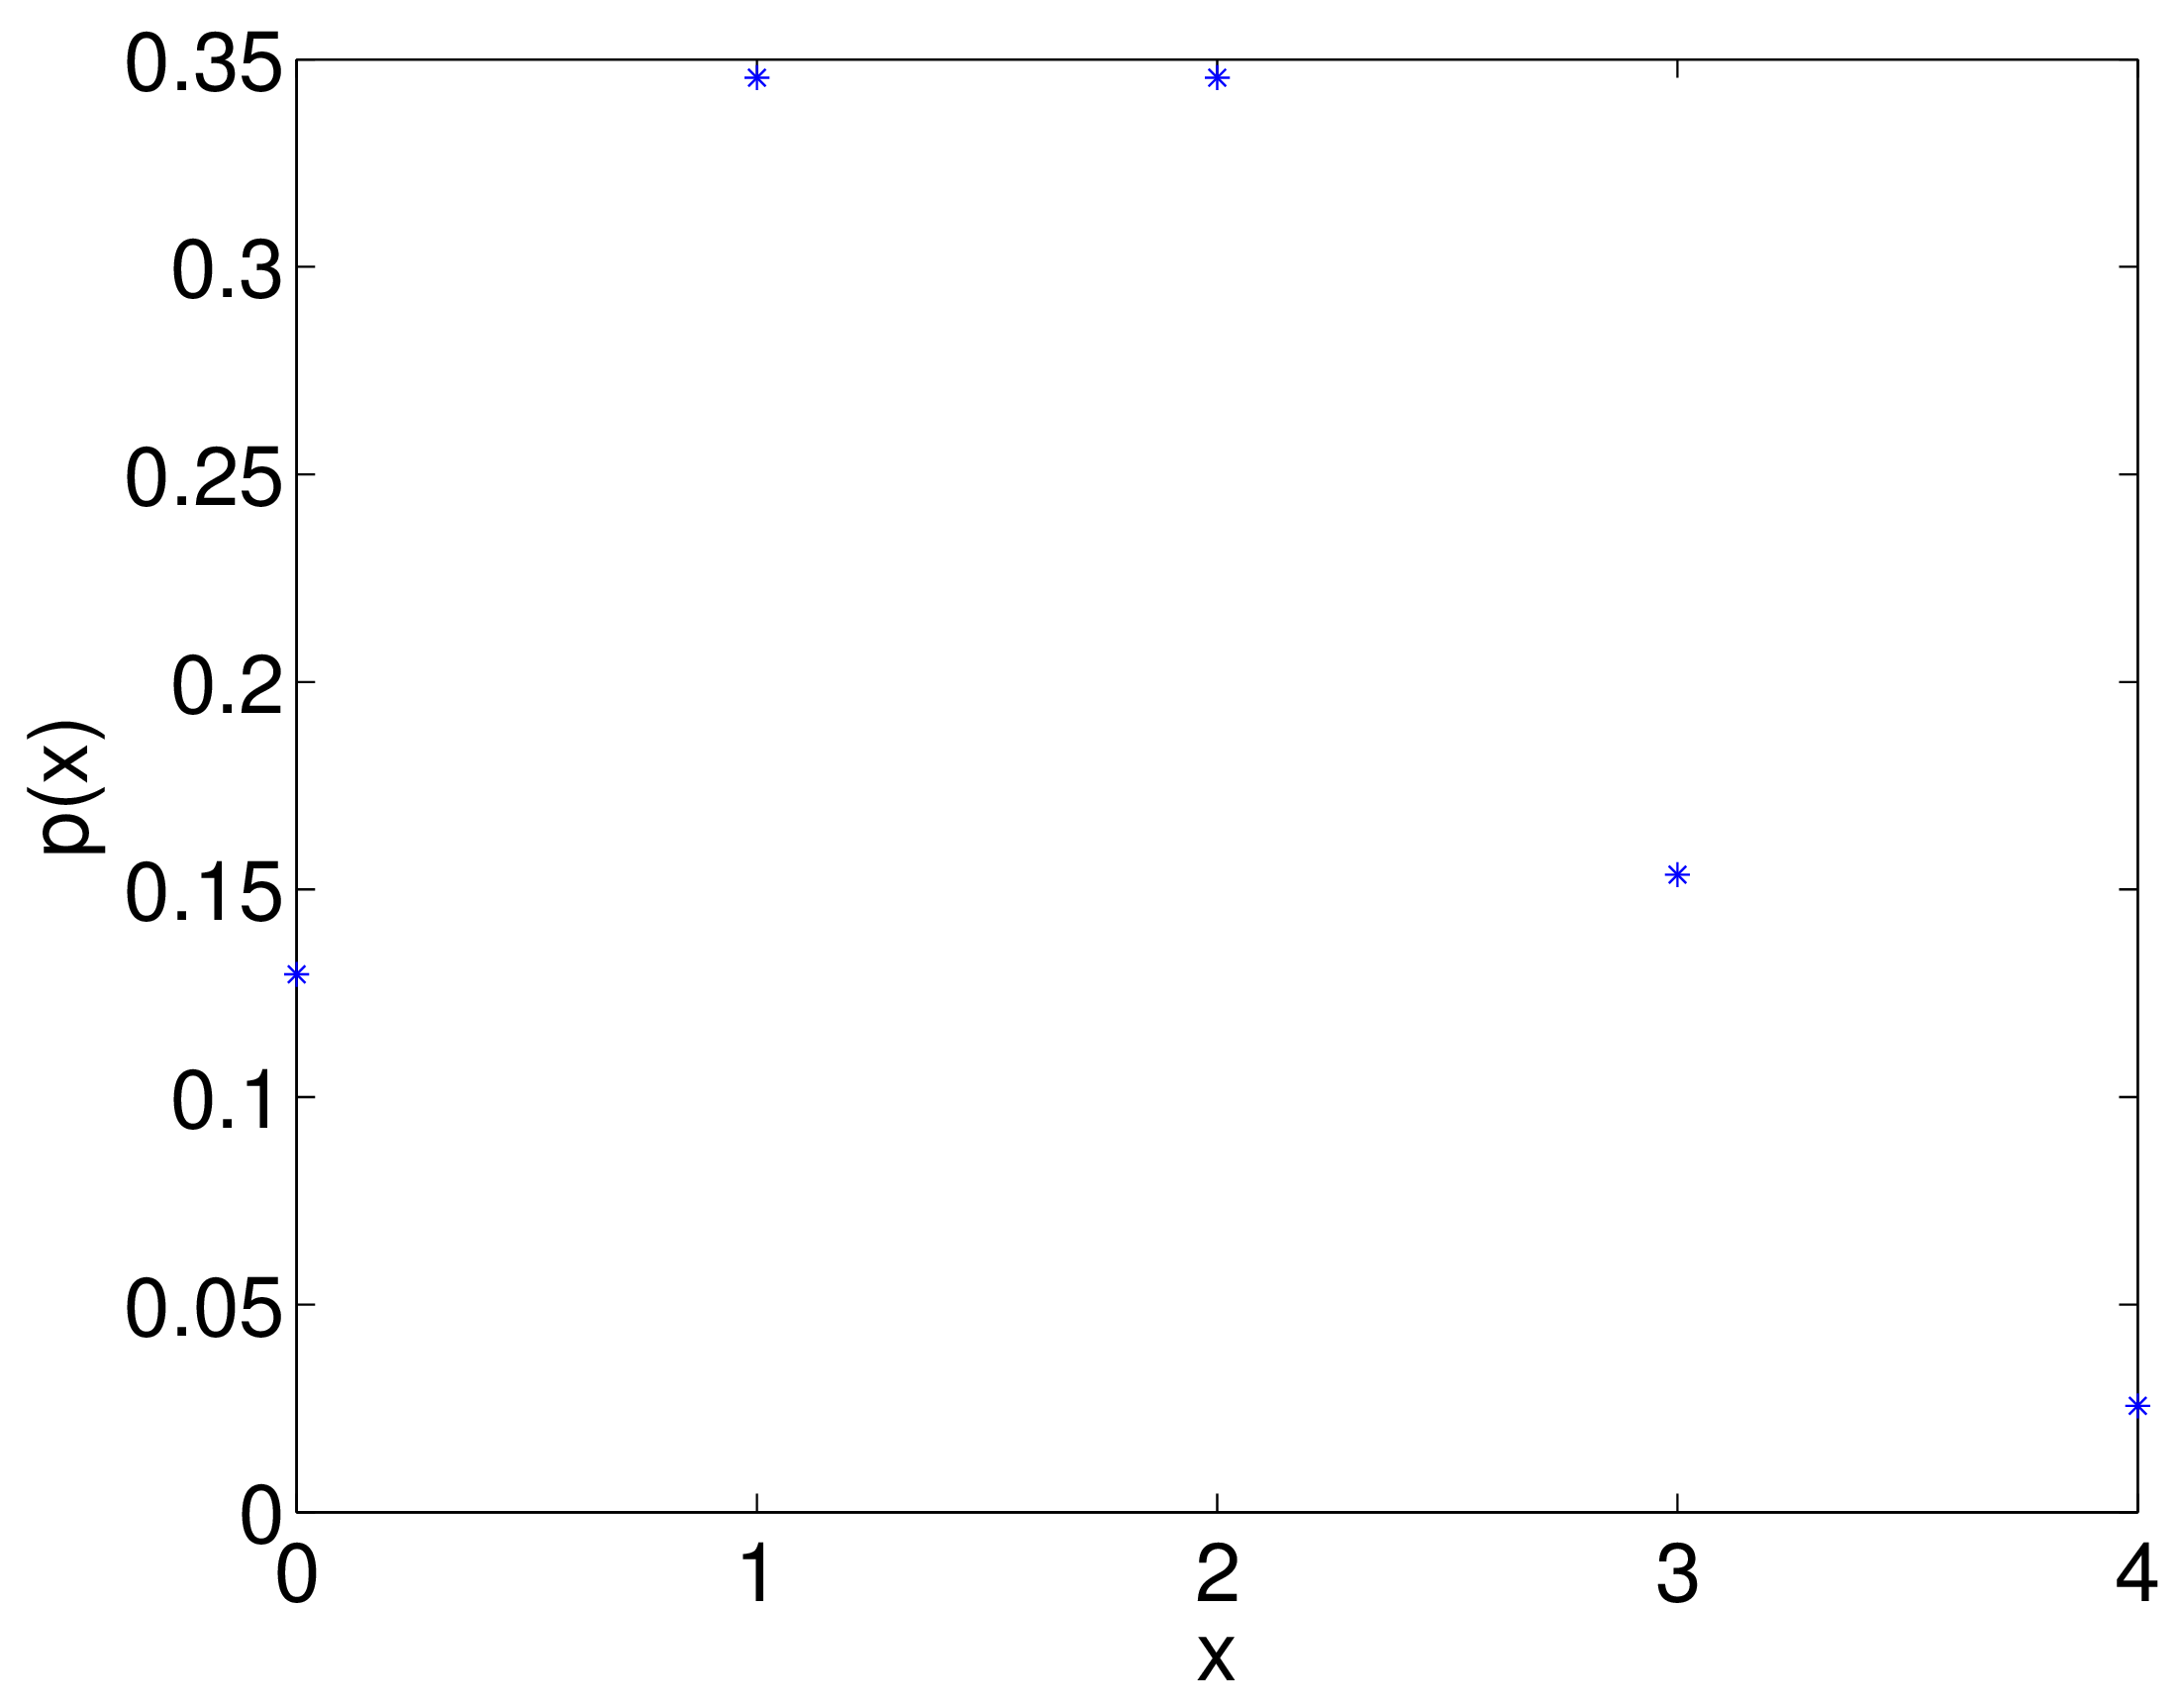
\includegraphics[scale=0.5]{bin45} }

\end{frame}

\begin{frame}[fragile]\frametitle{The binomial pdf}

\center{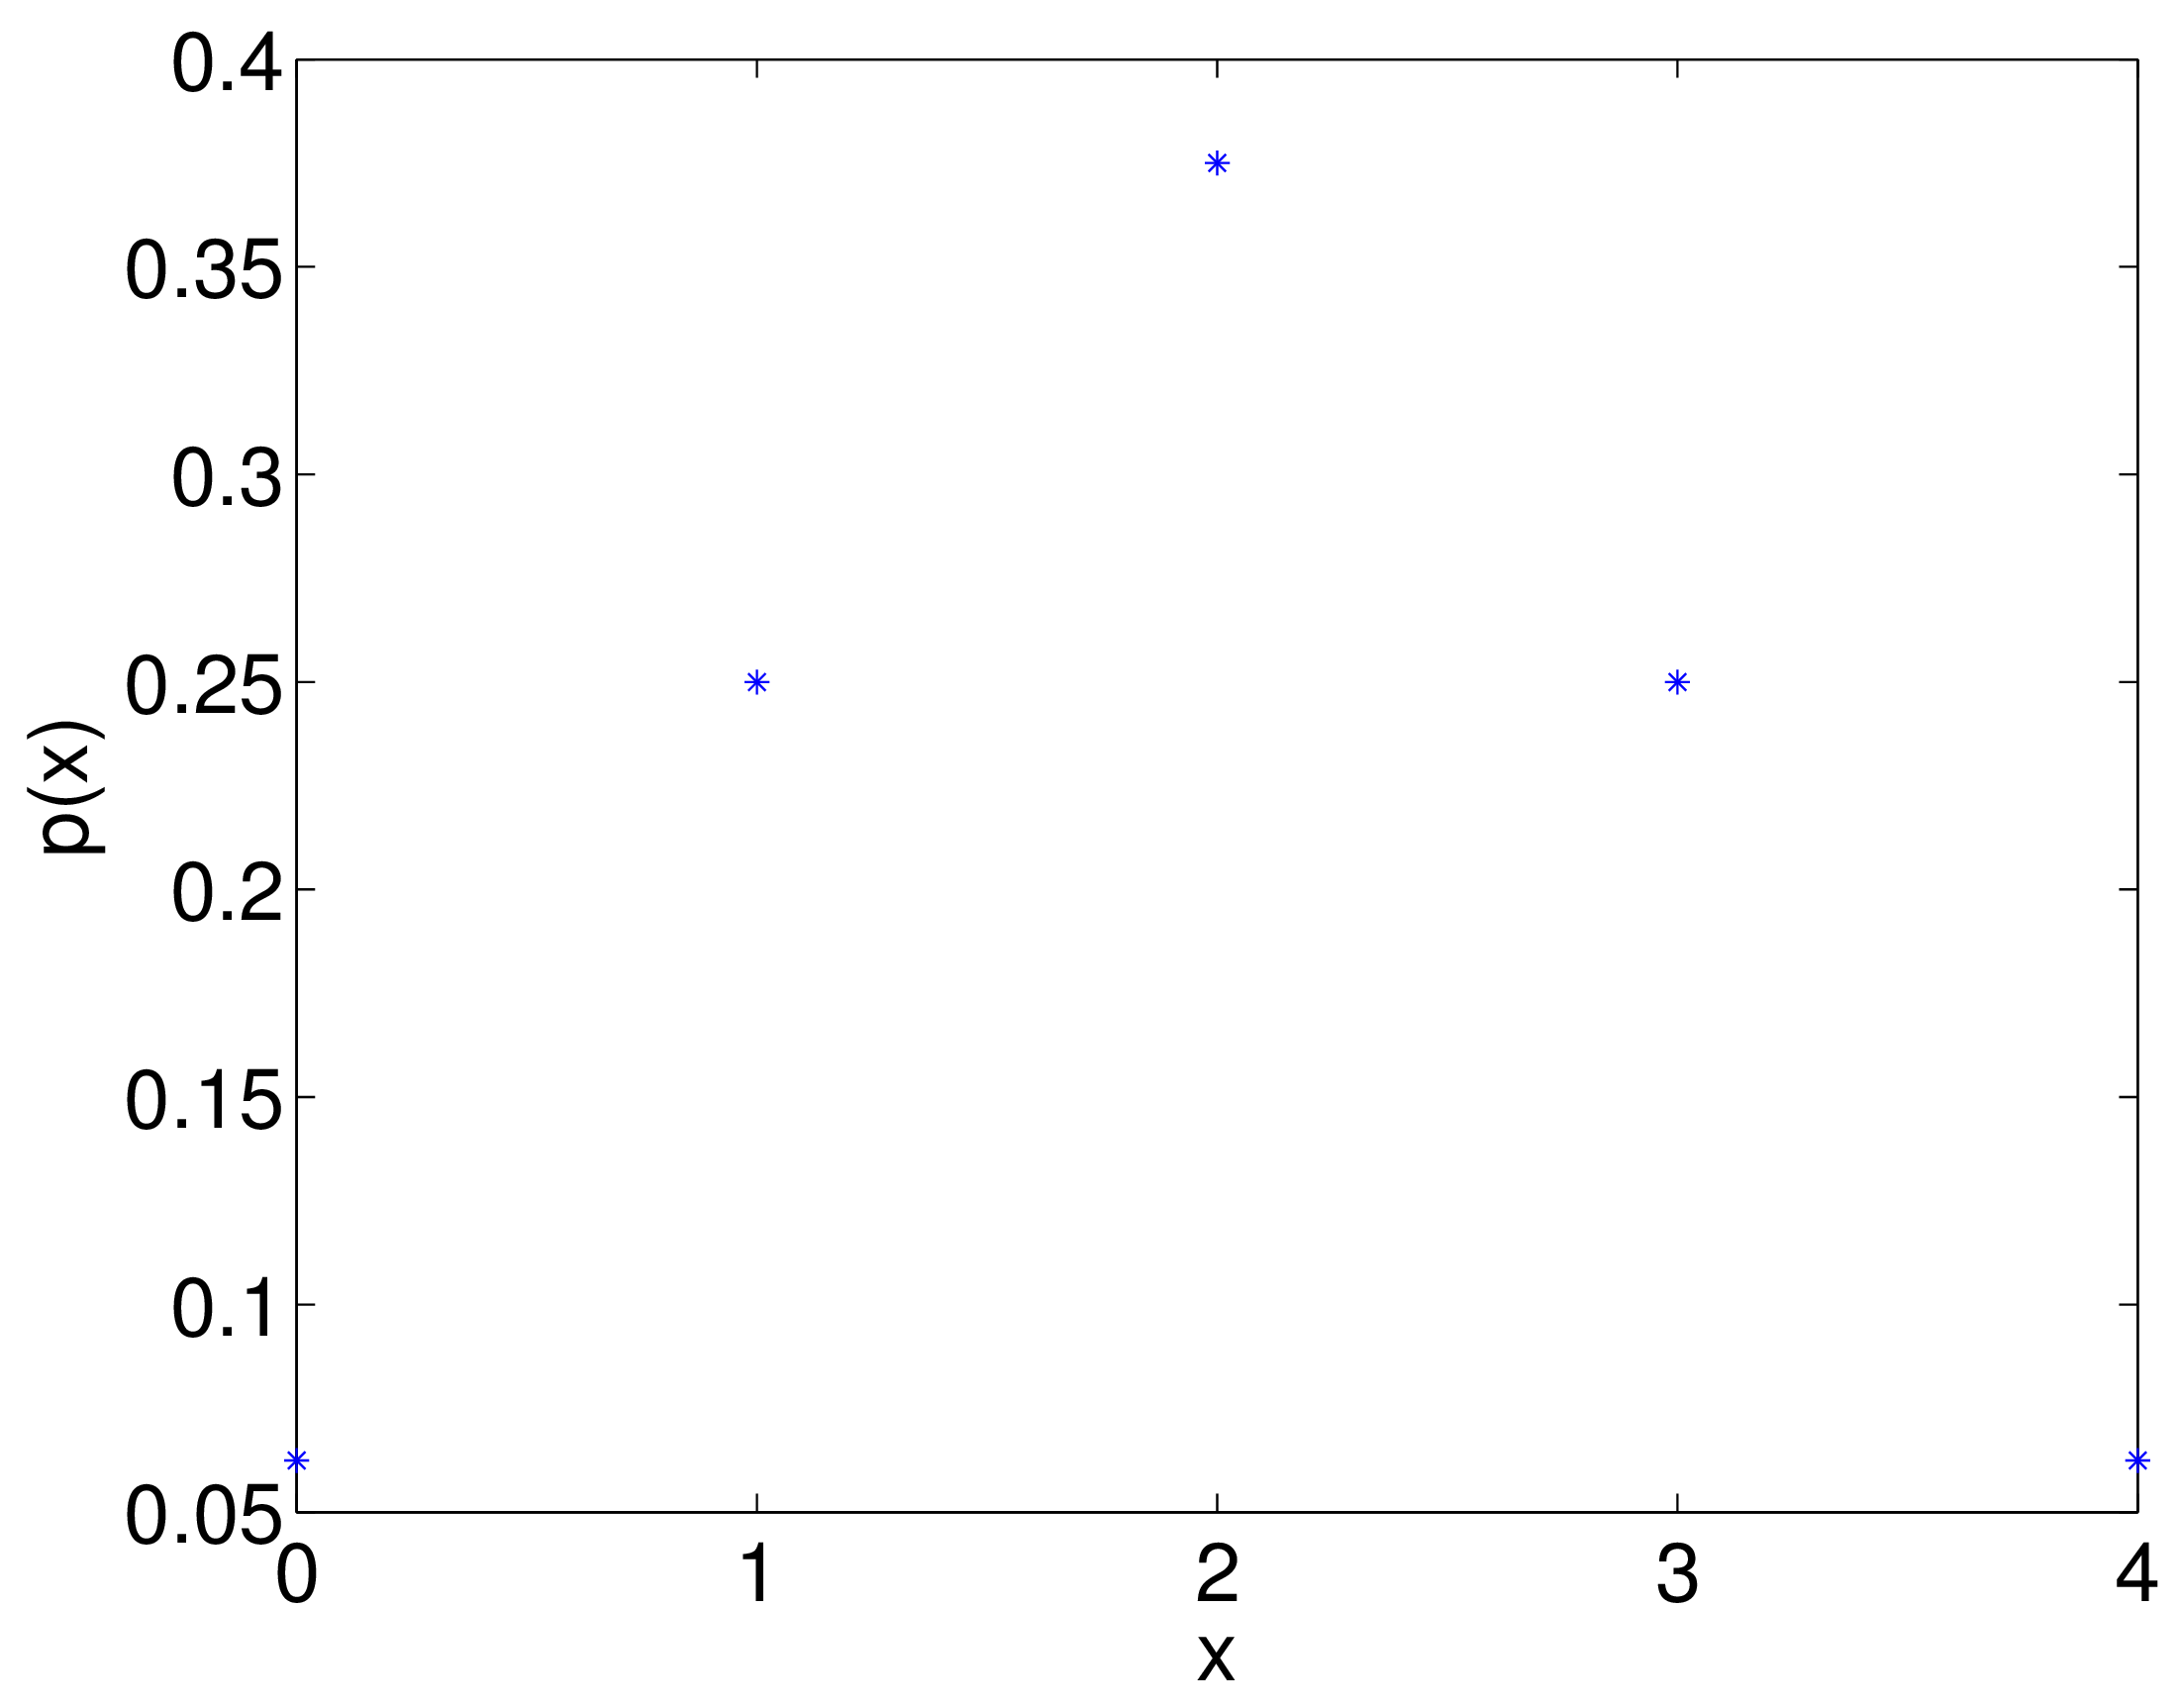
\includegraphics[scale=0.5]{bin46} }

\end{frame}

\begin{frame}[fragile]\frametitle{The binomial pdf}

\center{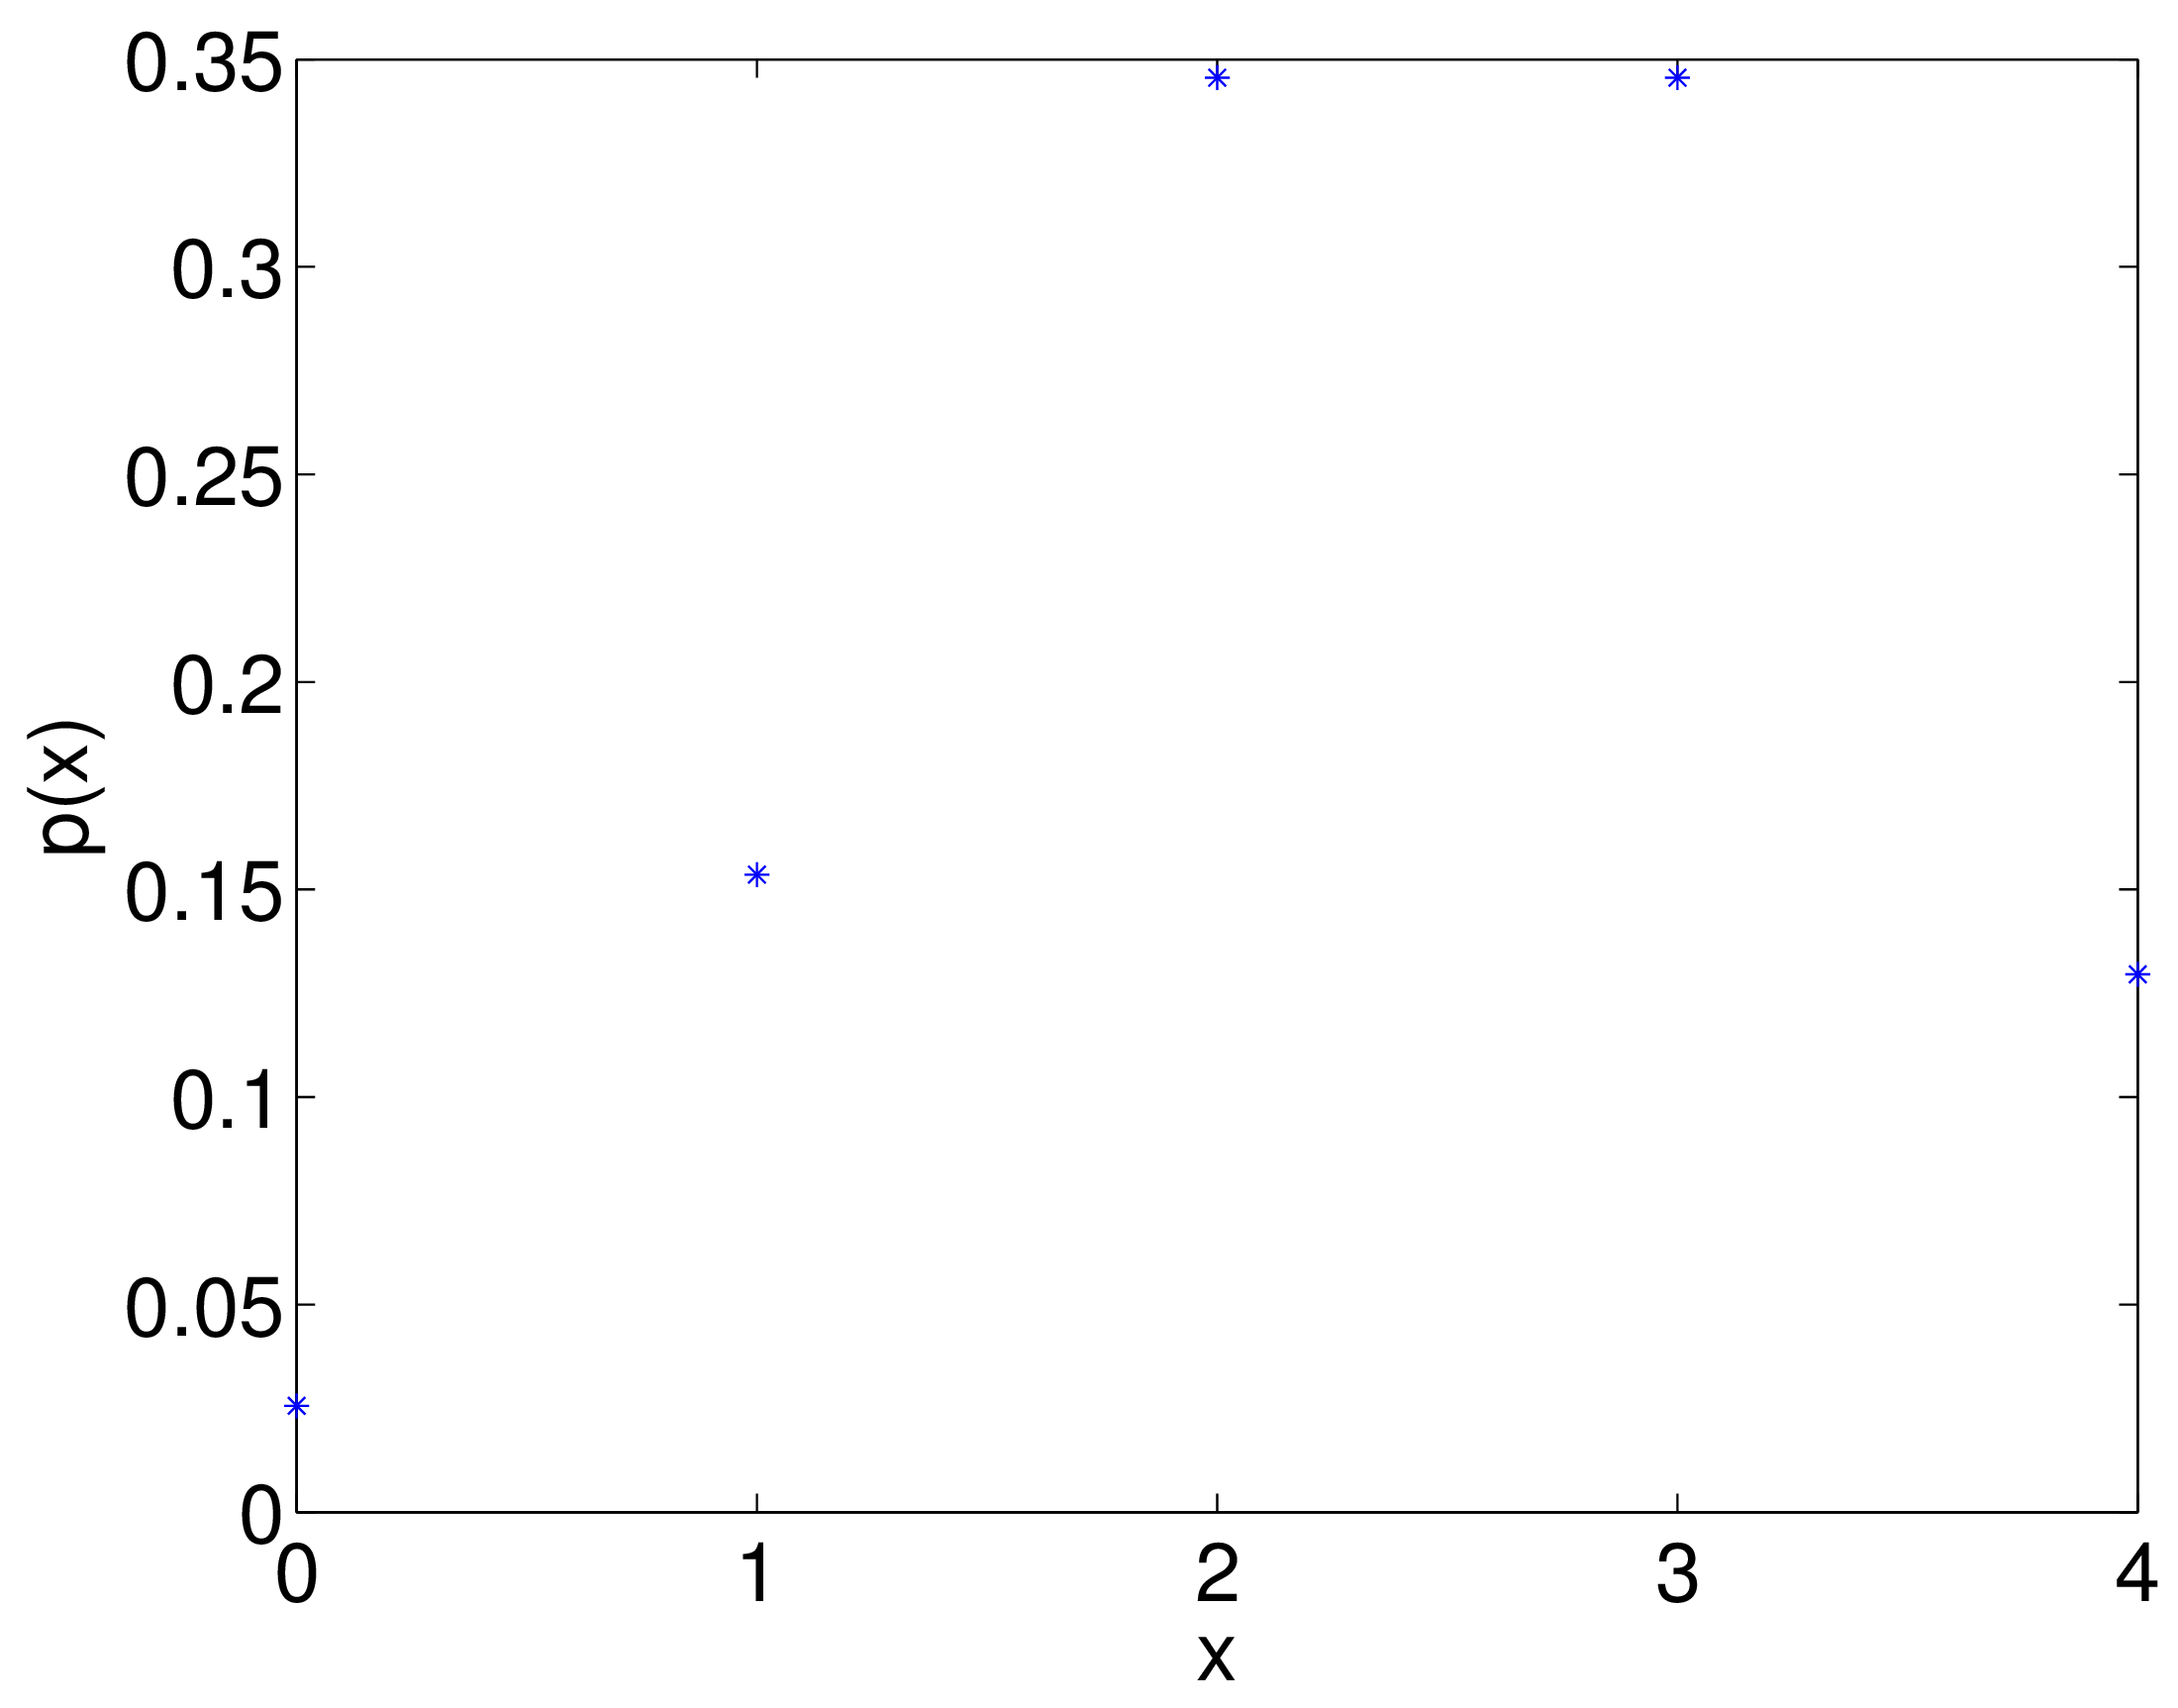
\includegraphics[scale=0.5]{bin47} }

\end{frame}

\begin{frame}[fragile]\frametitle{The binomial pdf}

\center{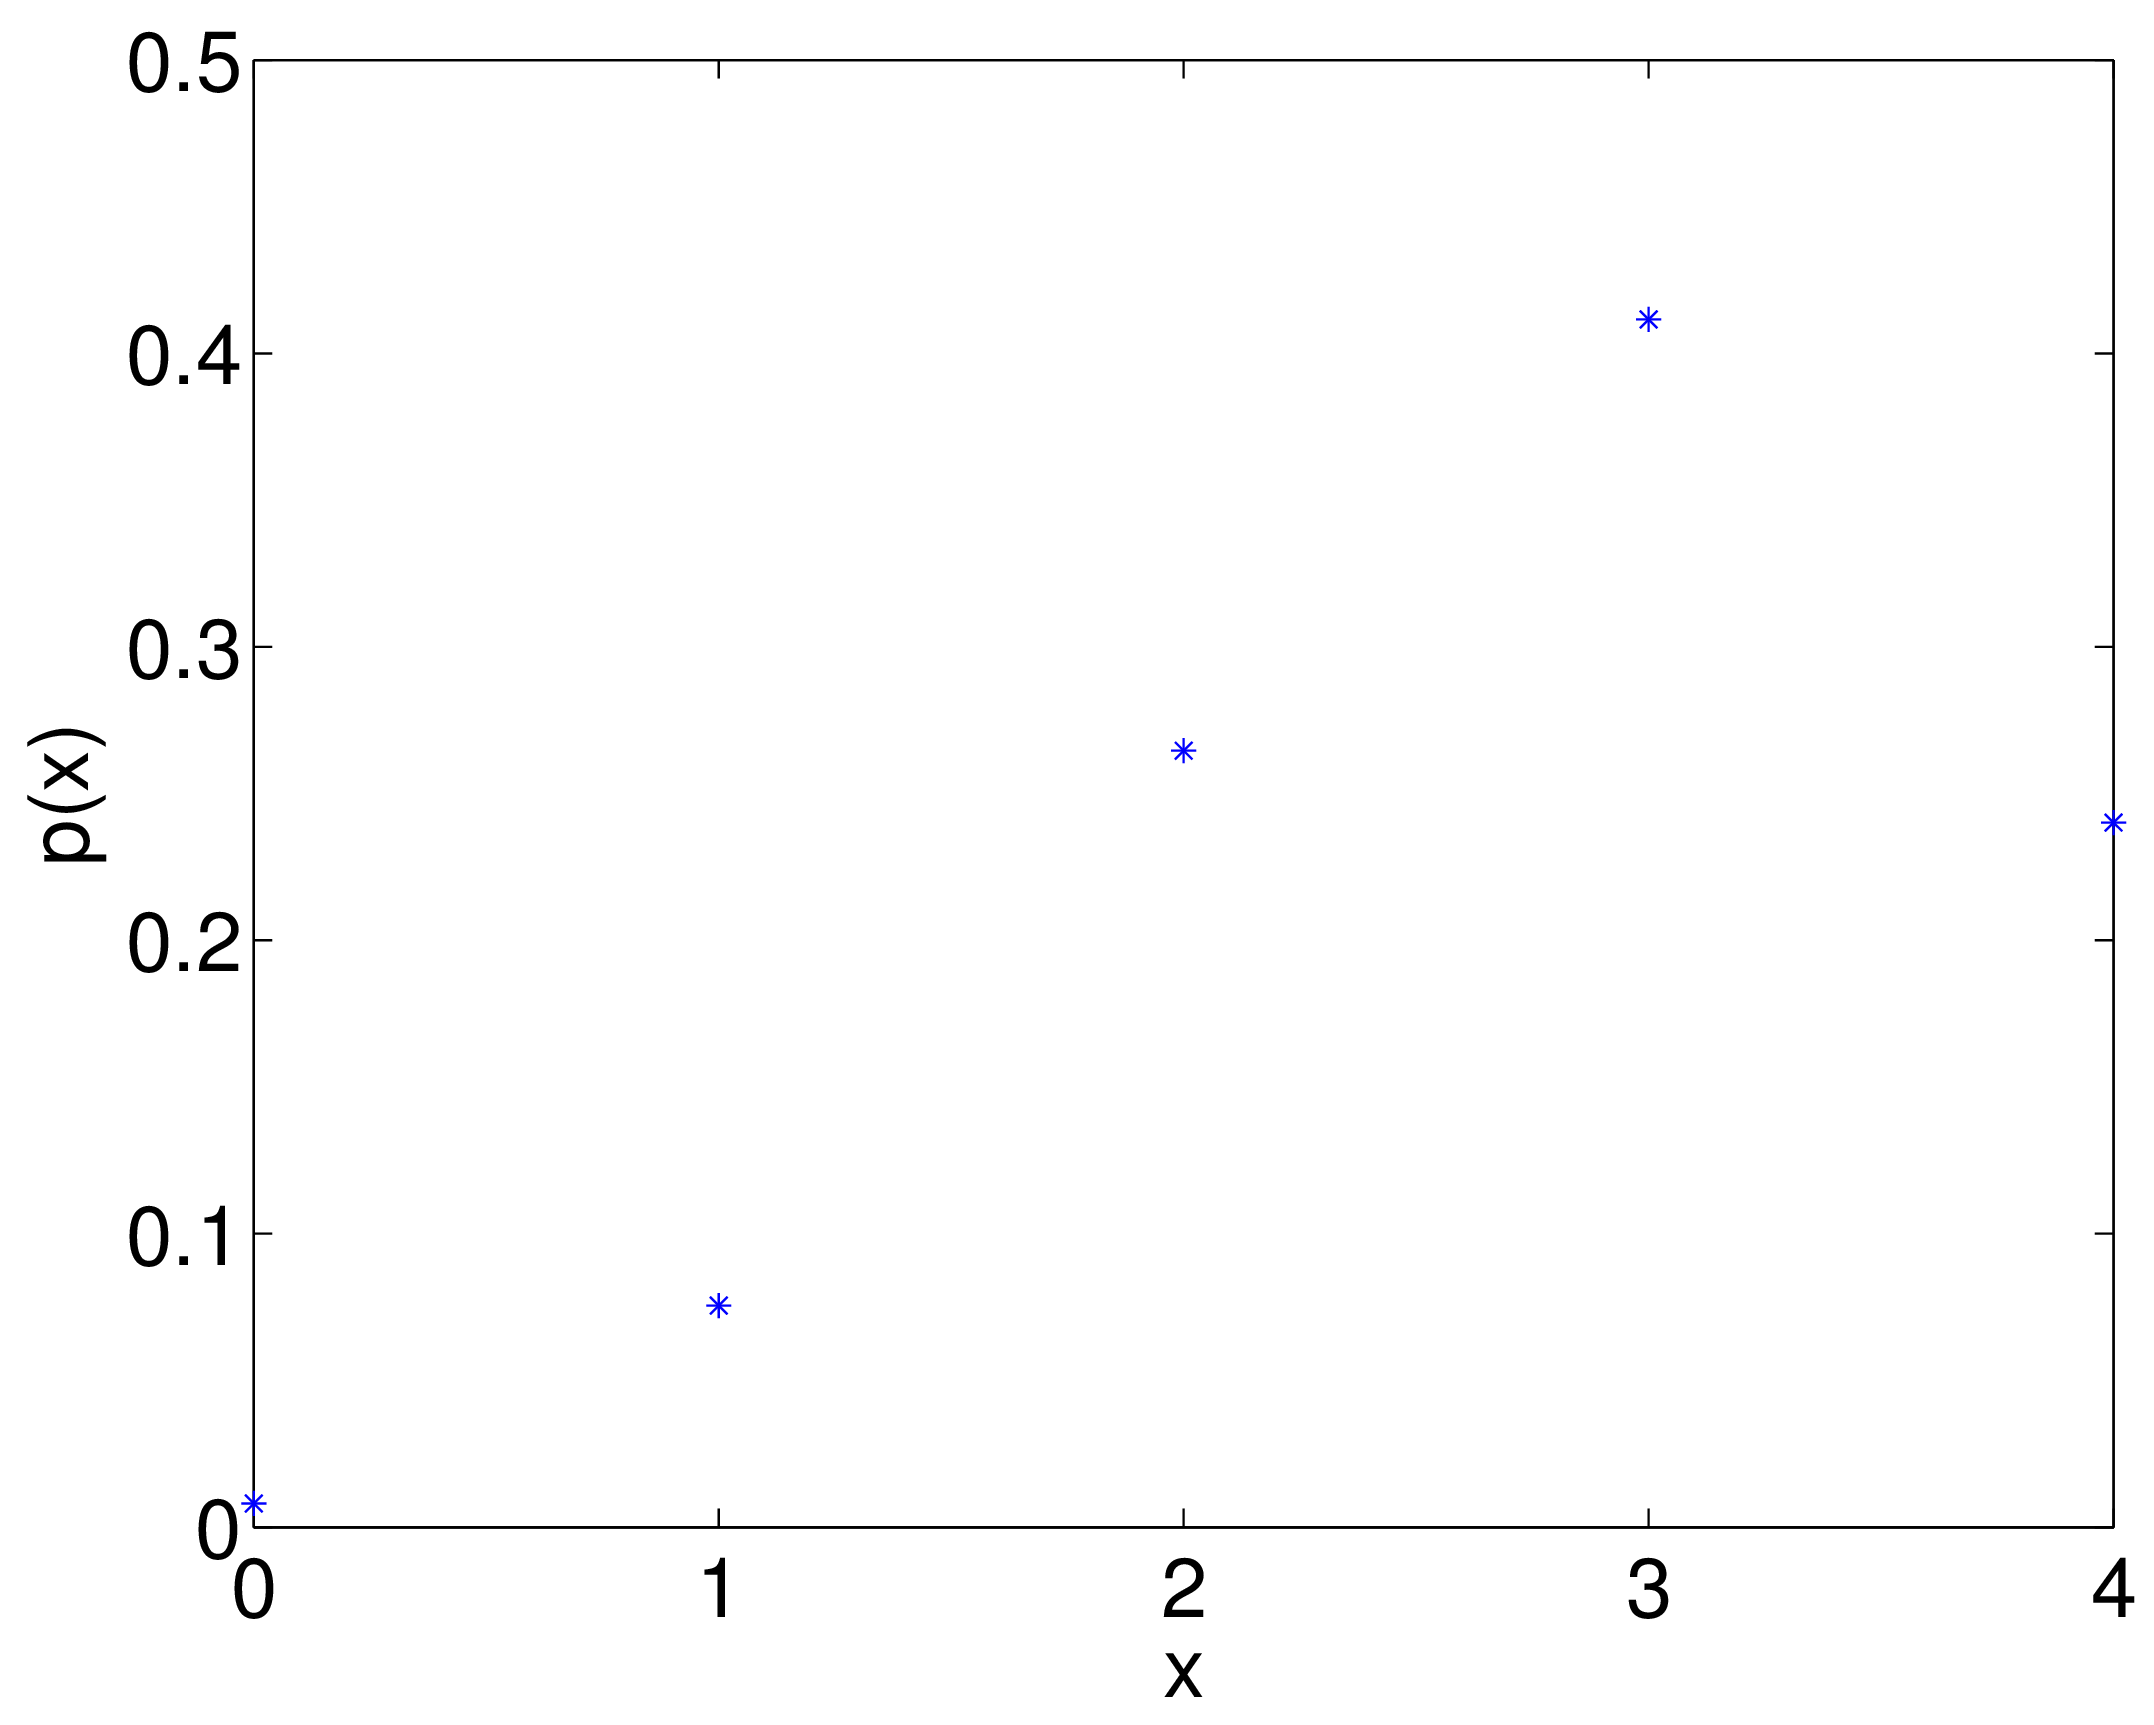
\includegraphics[scale=0.5]{bin48} }

\end{frame}

\begin{frame}[fragile]\frametitle{The binomial pdf}

\center{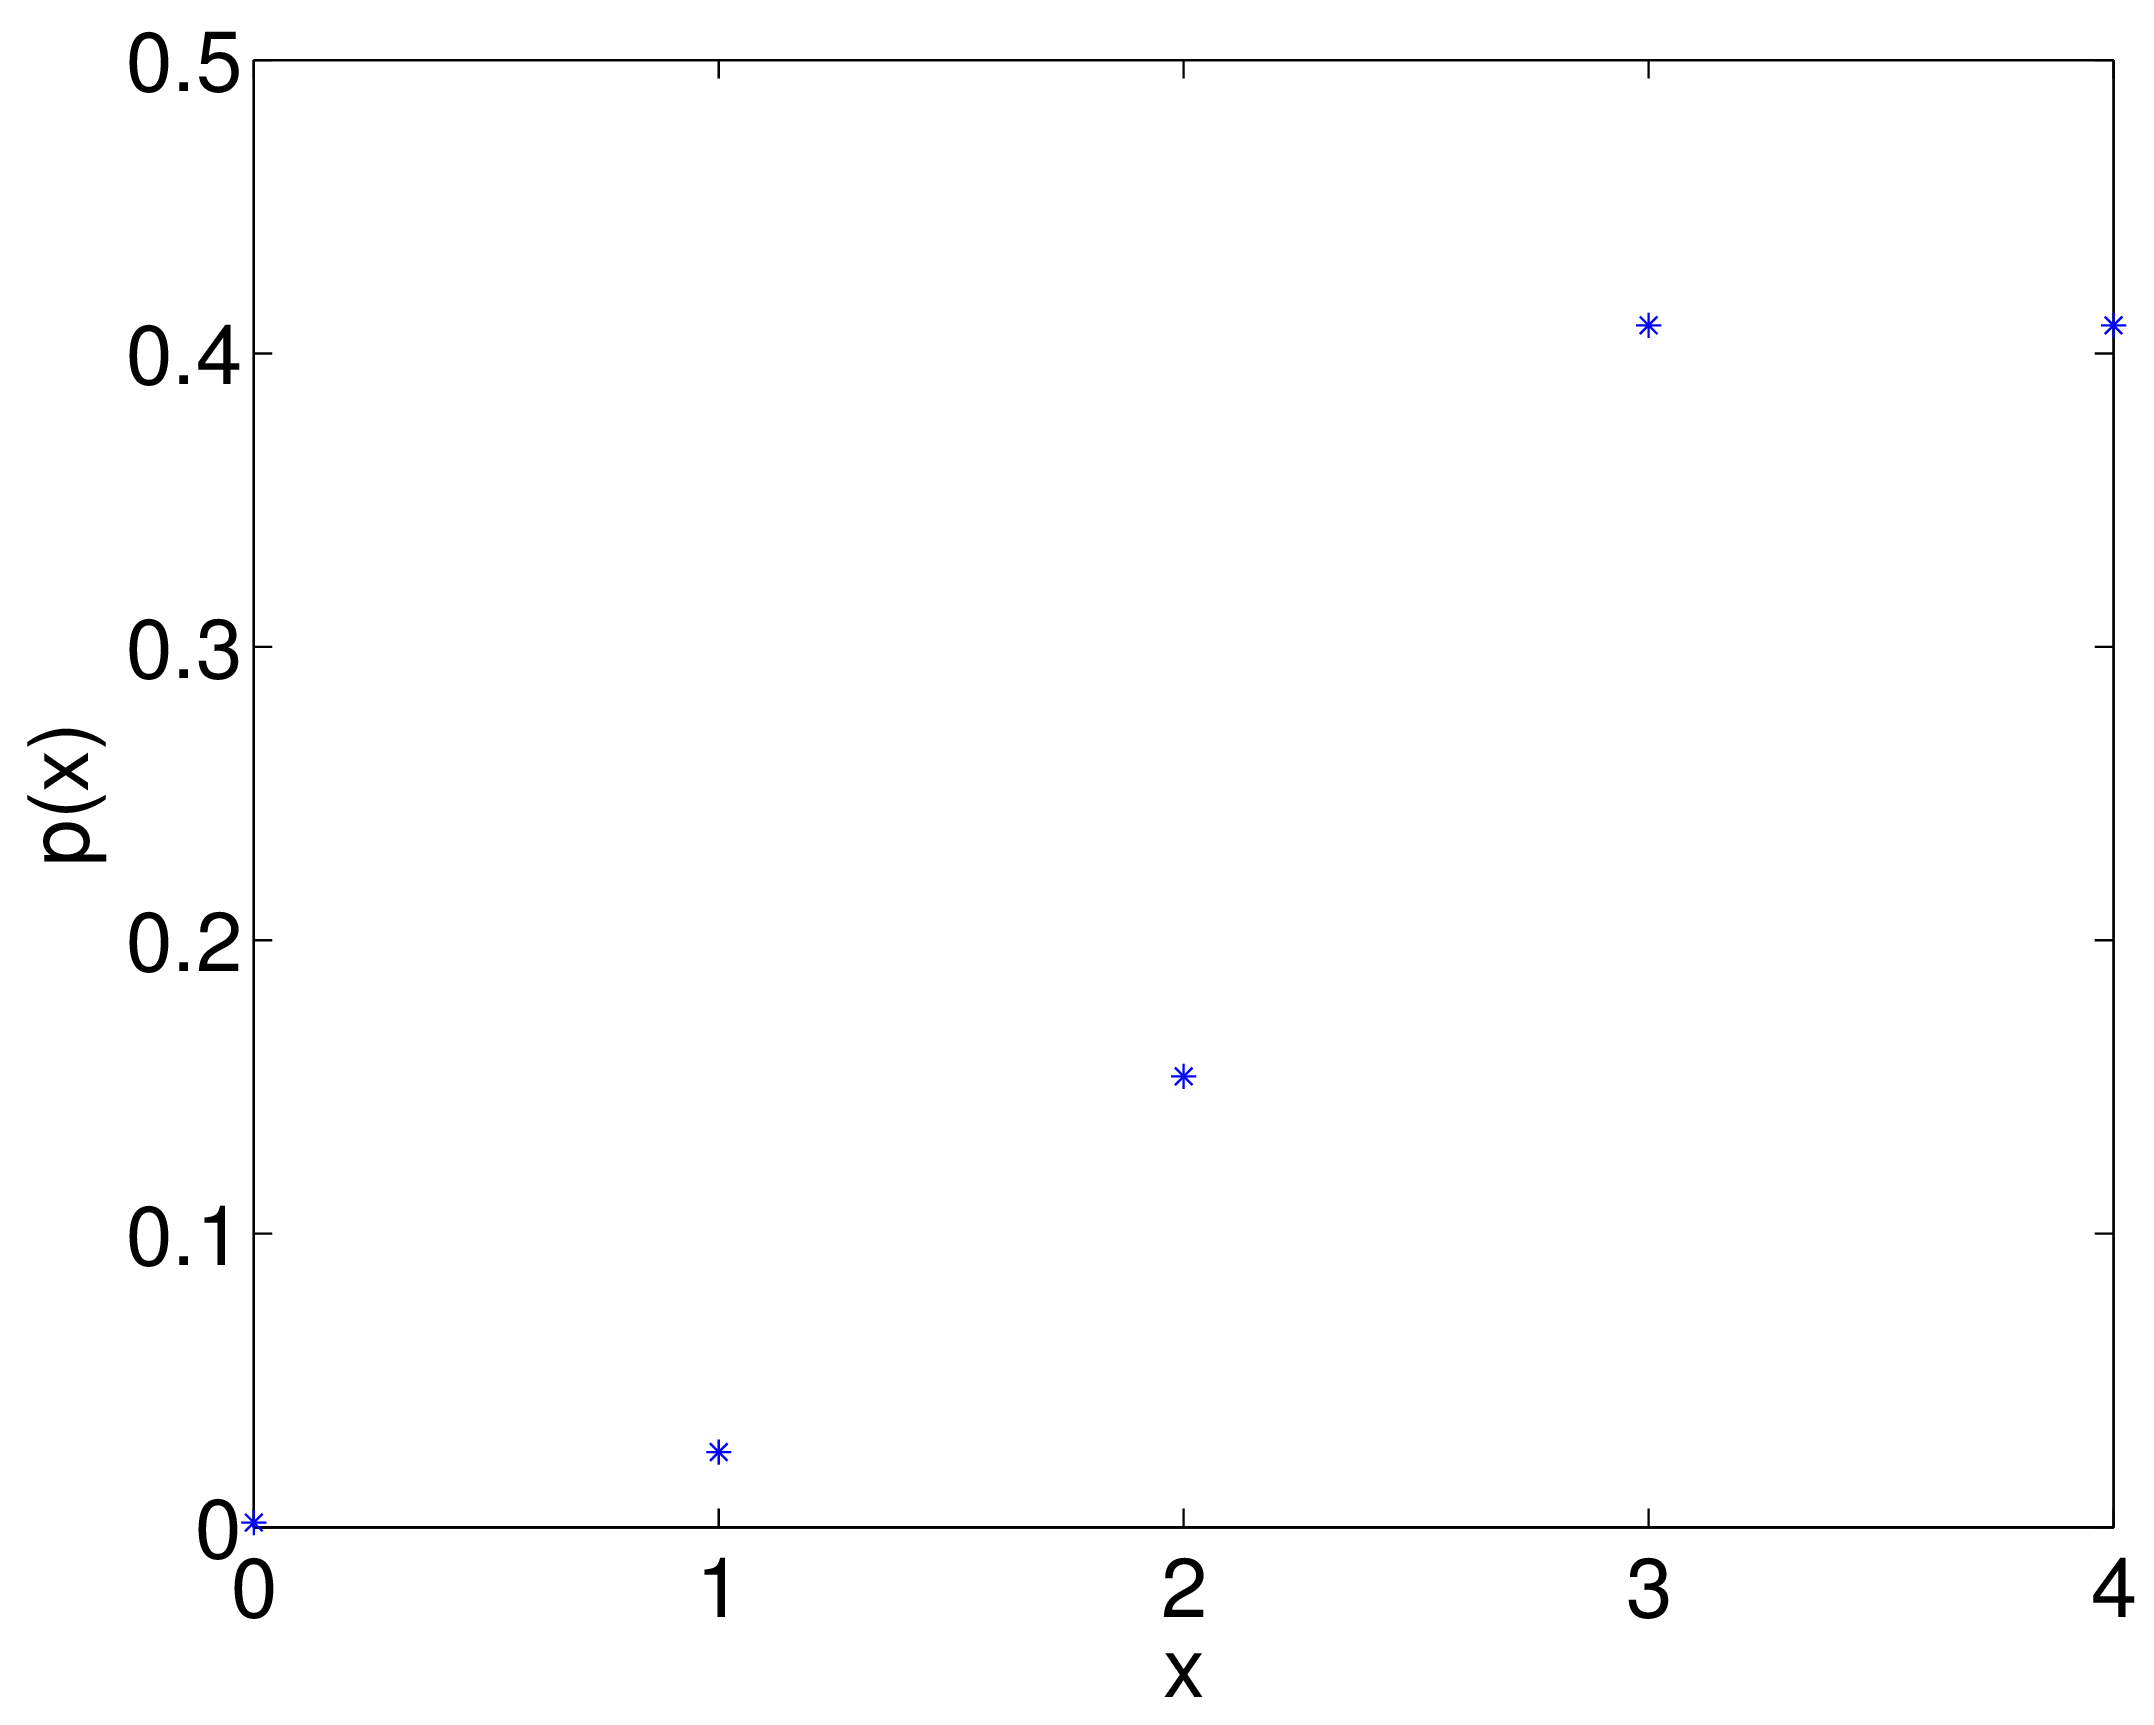
\includegraphics[scale=0.5]{bin49} }

\end{frame}


\begin{frame}[fragile]\frametitle{The binomial pdf}

\center{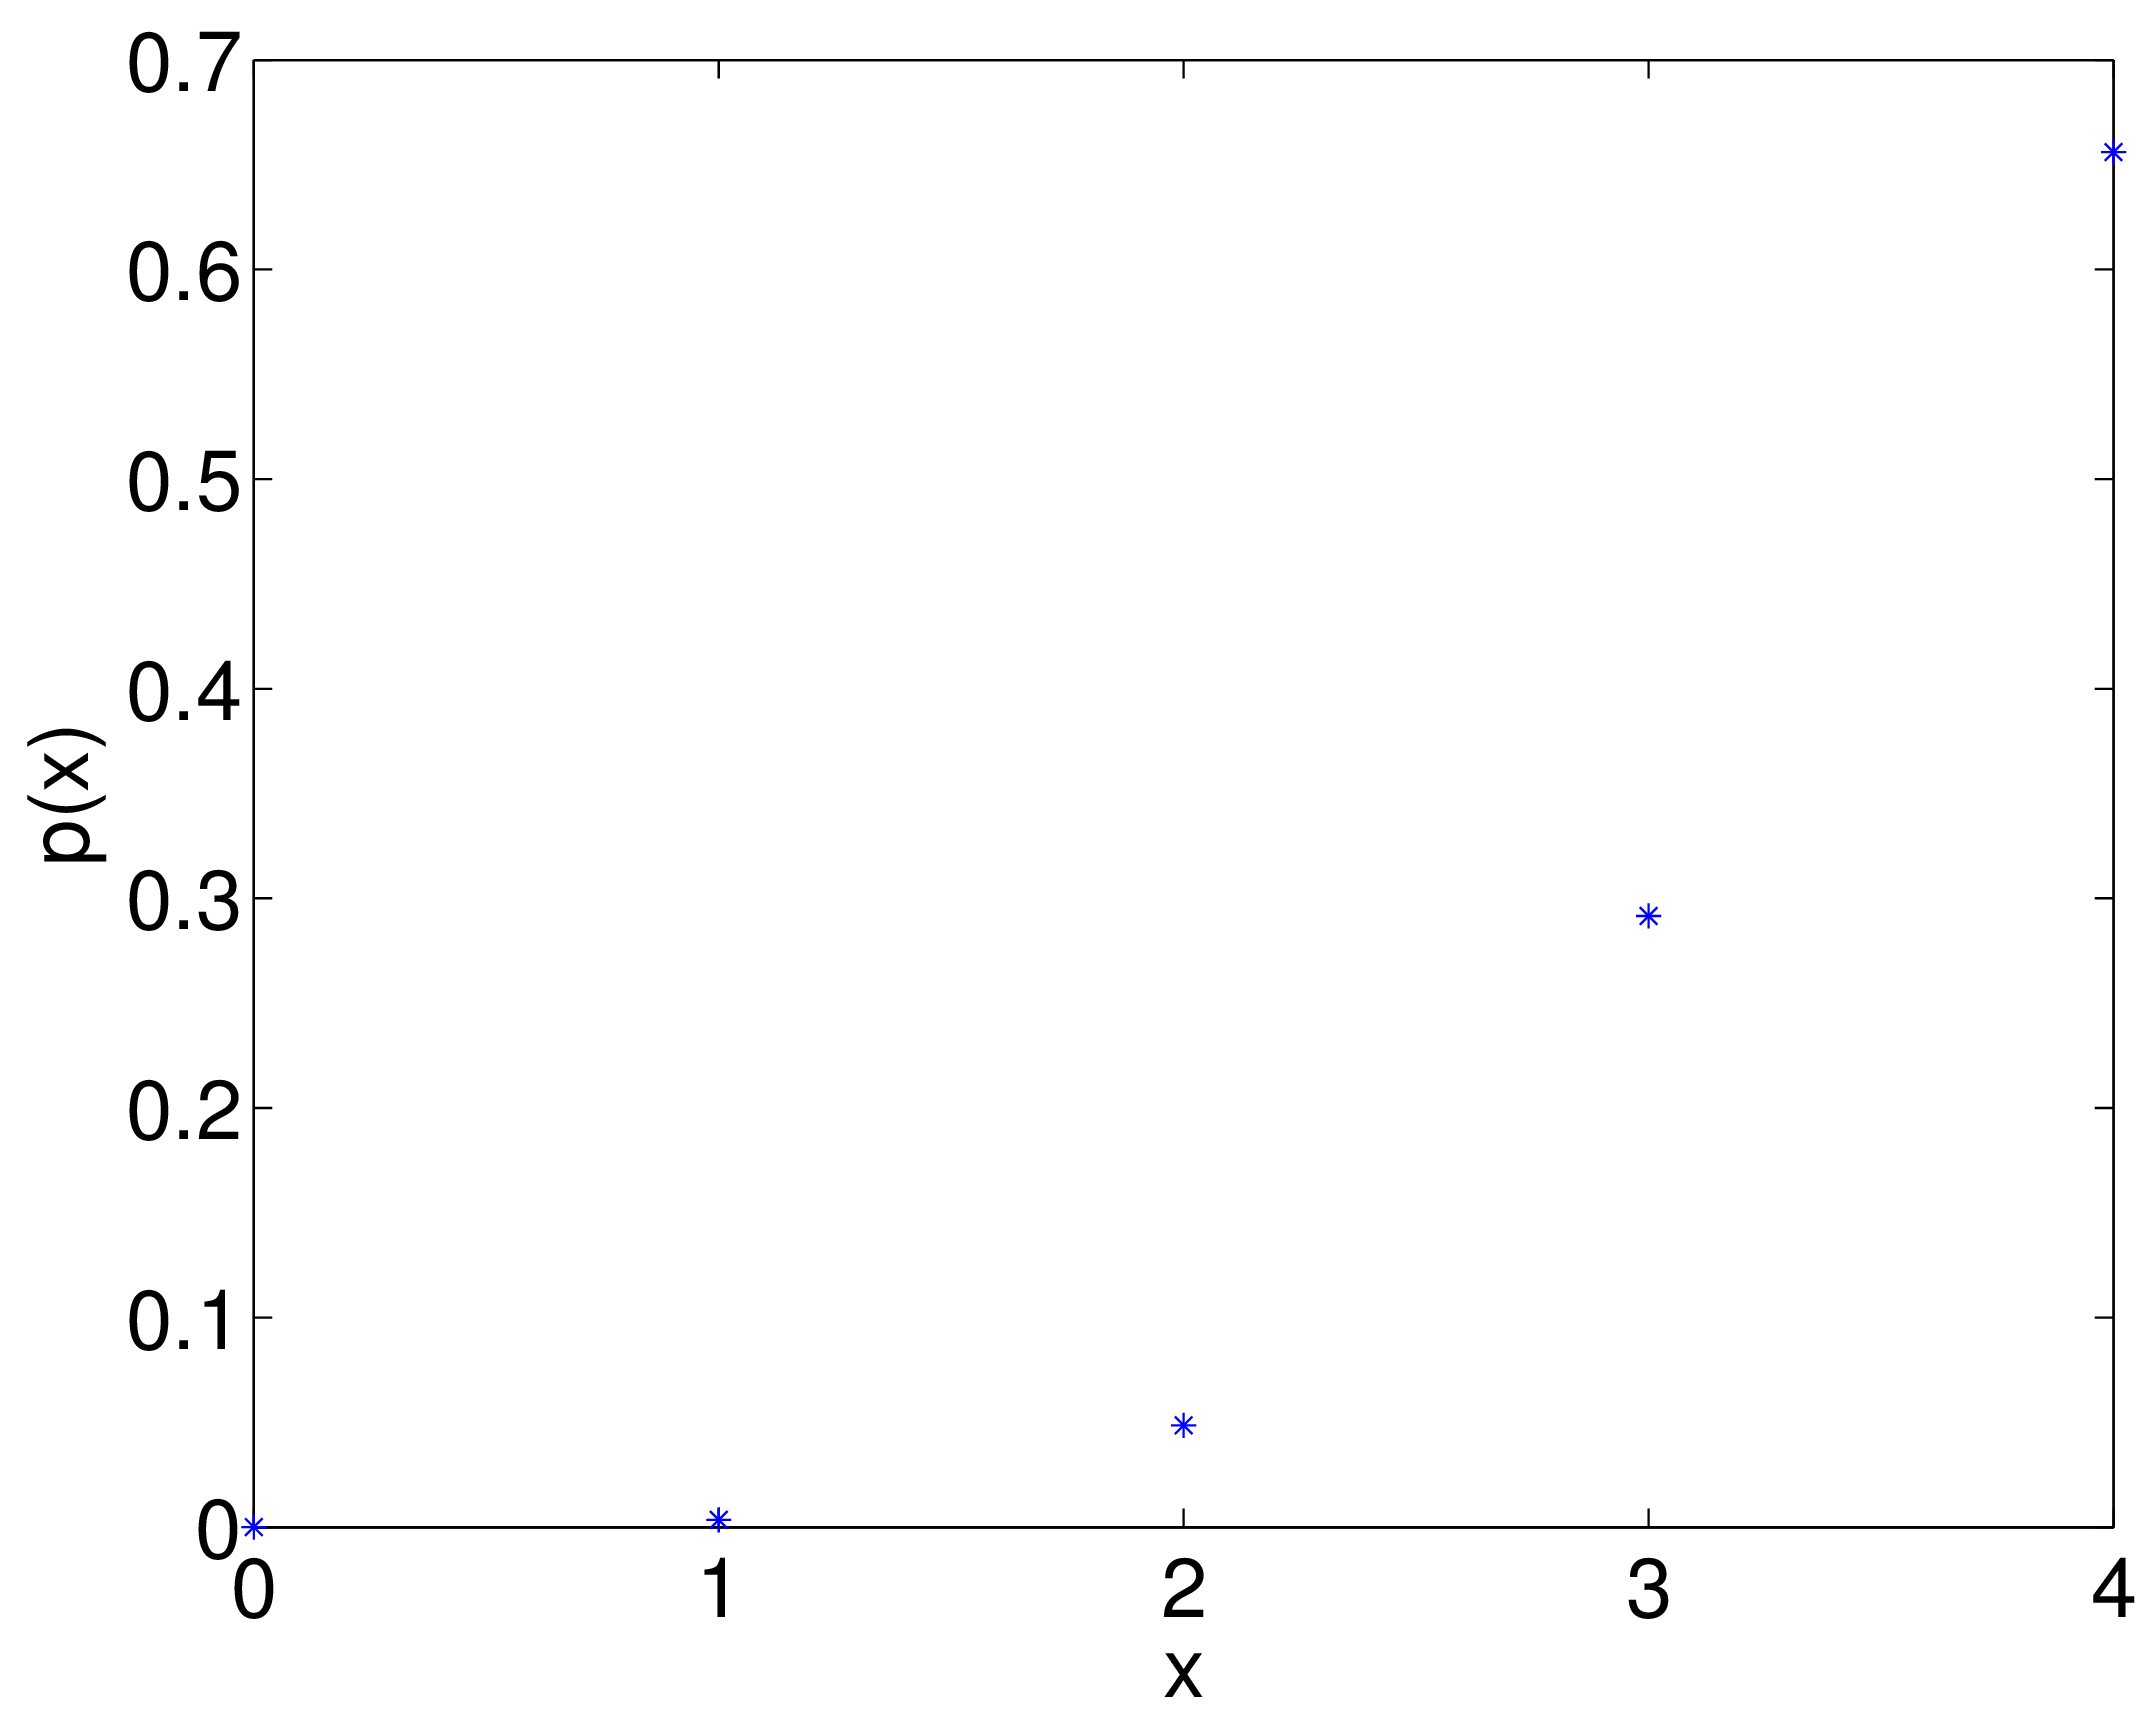
\includegraphics[scale=0.5]{bin410} }

\end{frame}

\begin{frame}[fragile]\frametitle{The binomial pdf}

\center{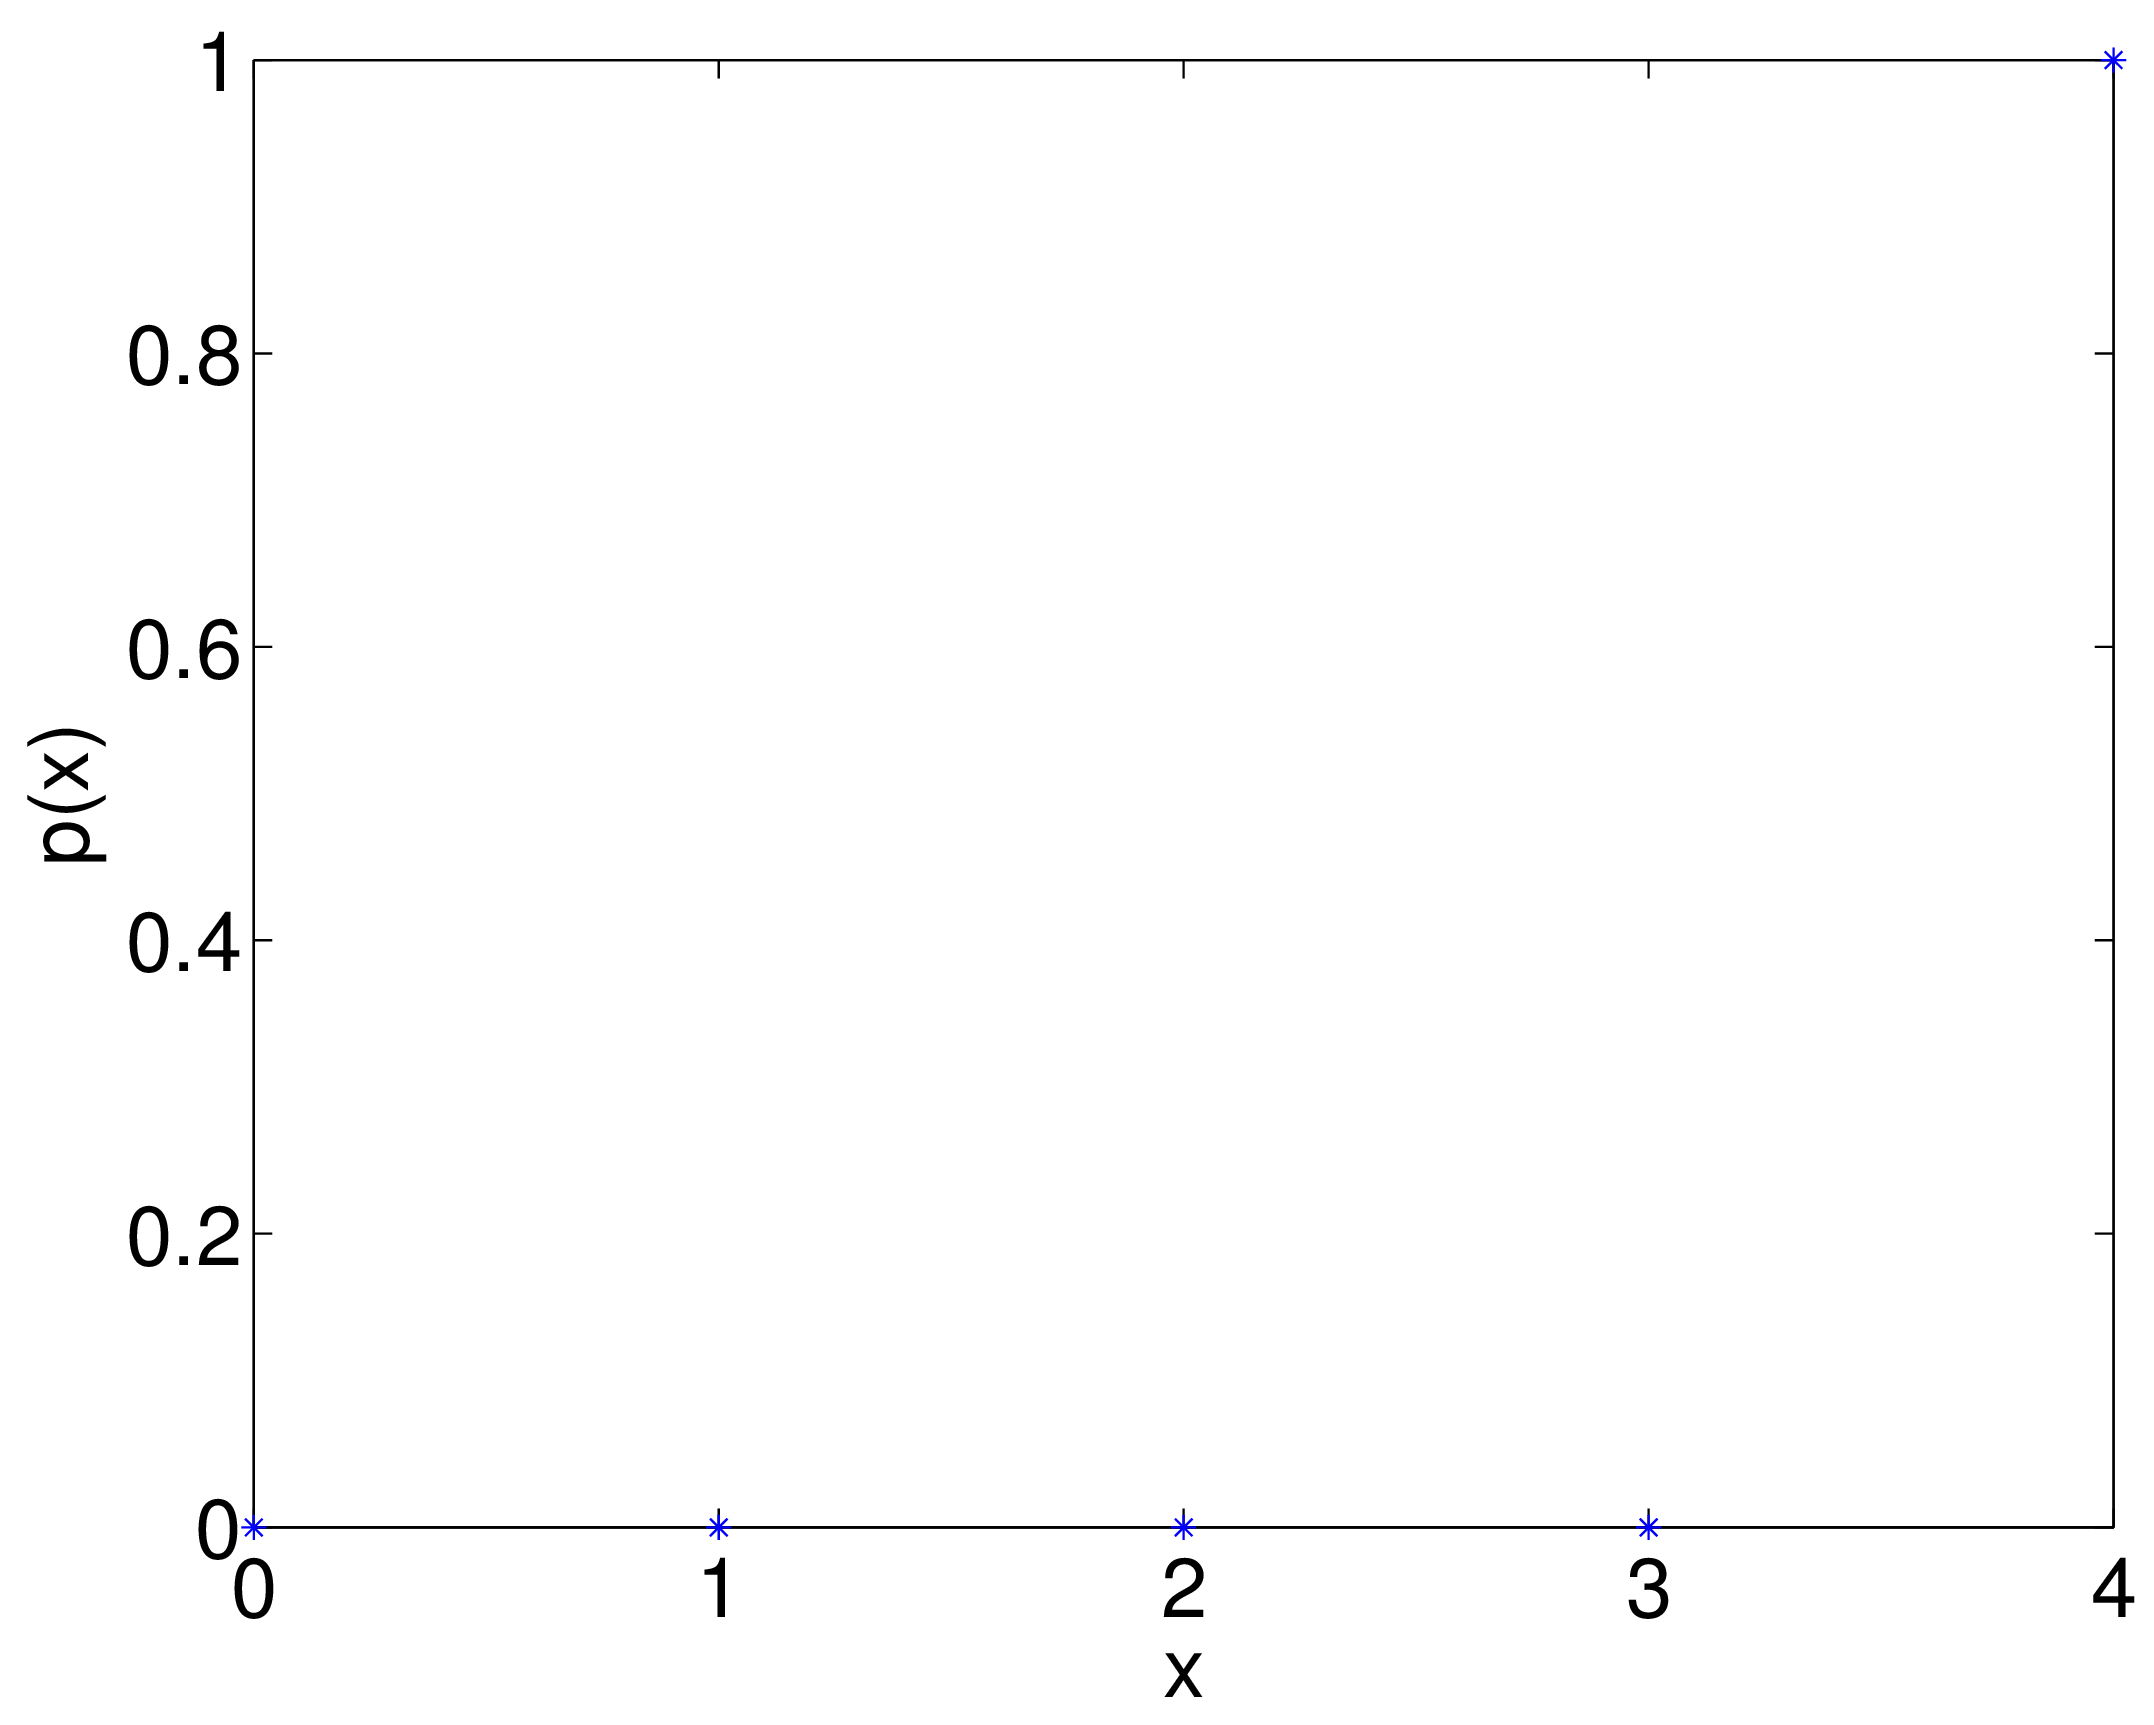
\includegraphics[scale=0.5]{bin411} }

\end{frame}


\begin{frame}[fragile]\frametitle{Matlab code}

{\tiny

\begin{lstlisting}
 n=4;\\
 x=0:n;\\
 \textcolor{keyword}{for} i=1:11\\
   p = (i-1)*.1;\\
   y=binopdf(x,n,p);\\
   figure(i);\\
   plot(x,y,'*');\\
   h=gca;\\
   set(h,'FontSize',[20]);\\
   xlabel('x');  \\
   ylabel('p(x)'); \\
   filename = sprintf('bin4\%d',i);\\
   saveas(h,filename,'psc2') \\
 \textcolor{keyword}{end}
\end{lstlisting}
}
\end{frame}



\begin{frame}[fragile]\frametitle{The binomial pdf}

Fix $p=.4$ and vary $n$. 

\end{frame}




\begin{frame}[fragile]\frametitle{The binomial pdf}

\center{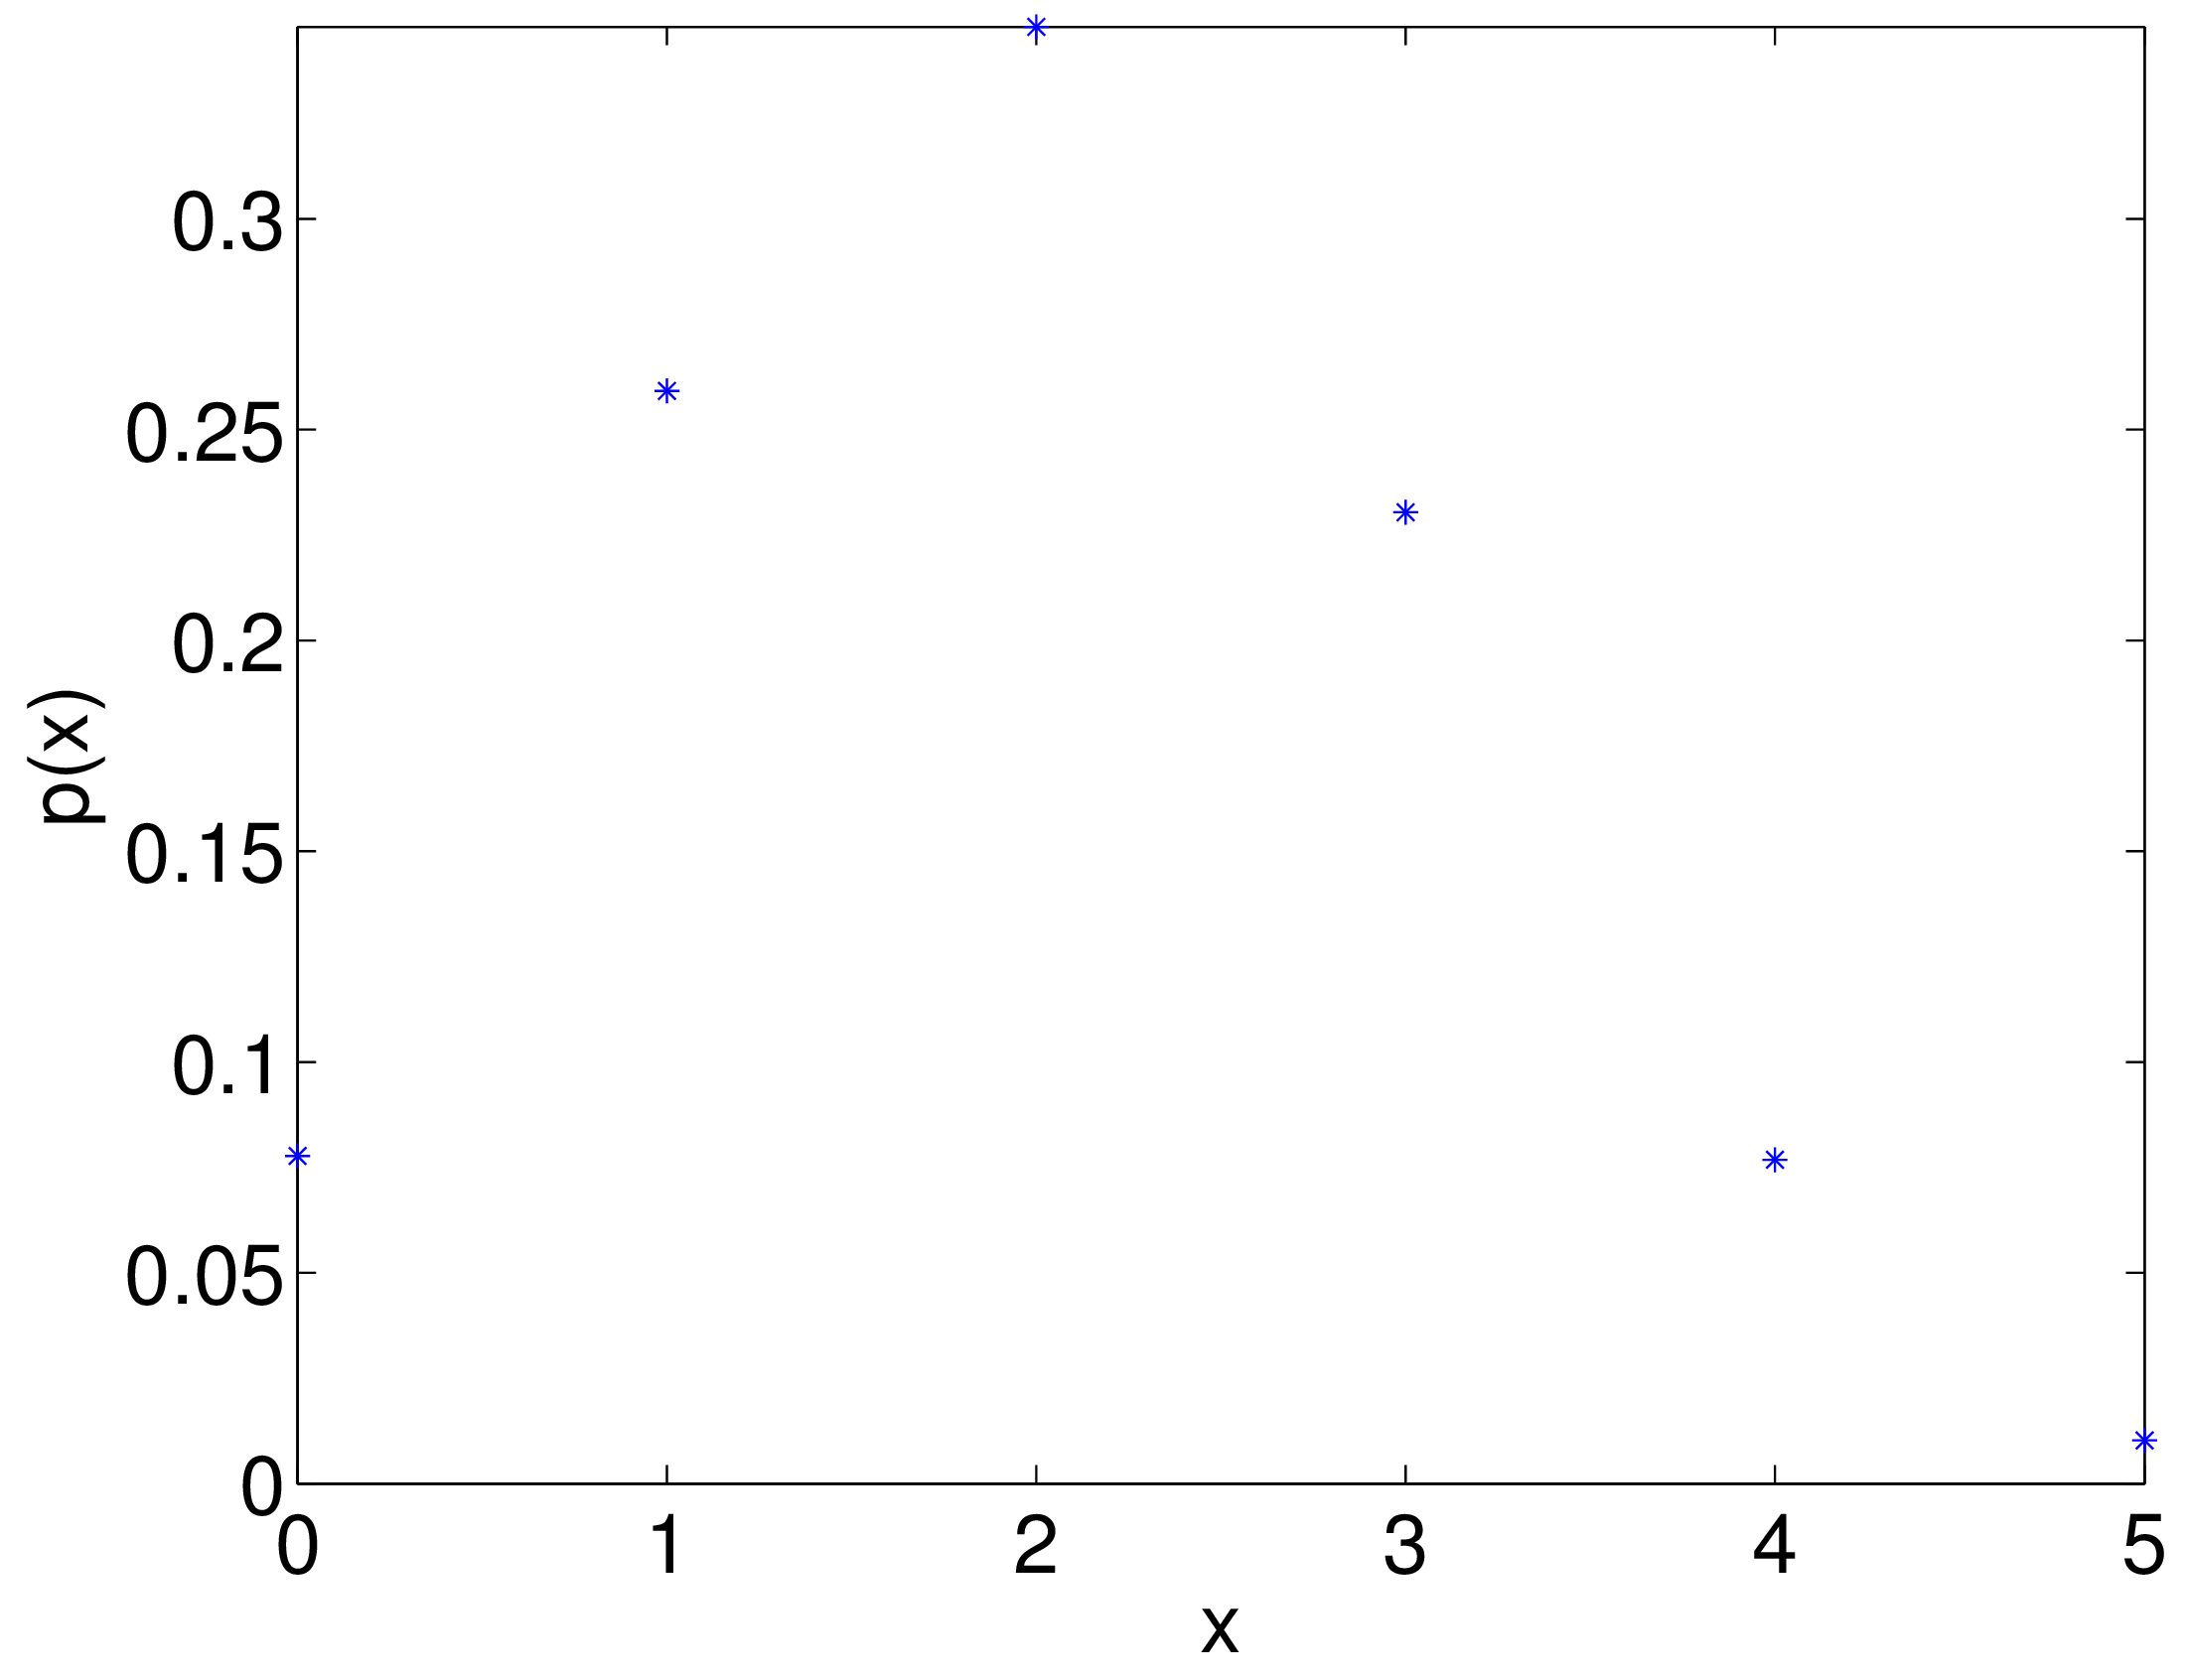
\includegraphics[scale=0.5]{vpbin1} }

\end{frame}

\begin{frame}[fragile]\frametitle{The binomial pdf}

\center{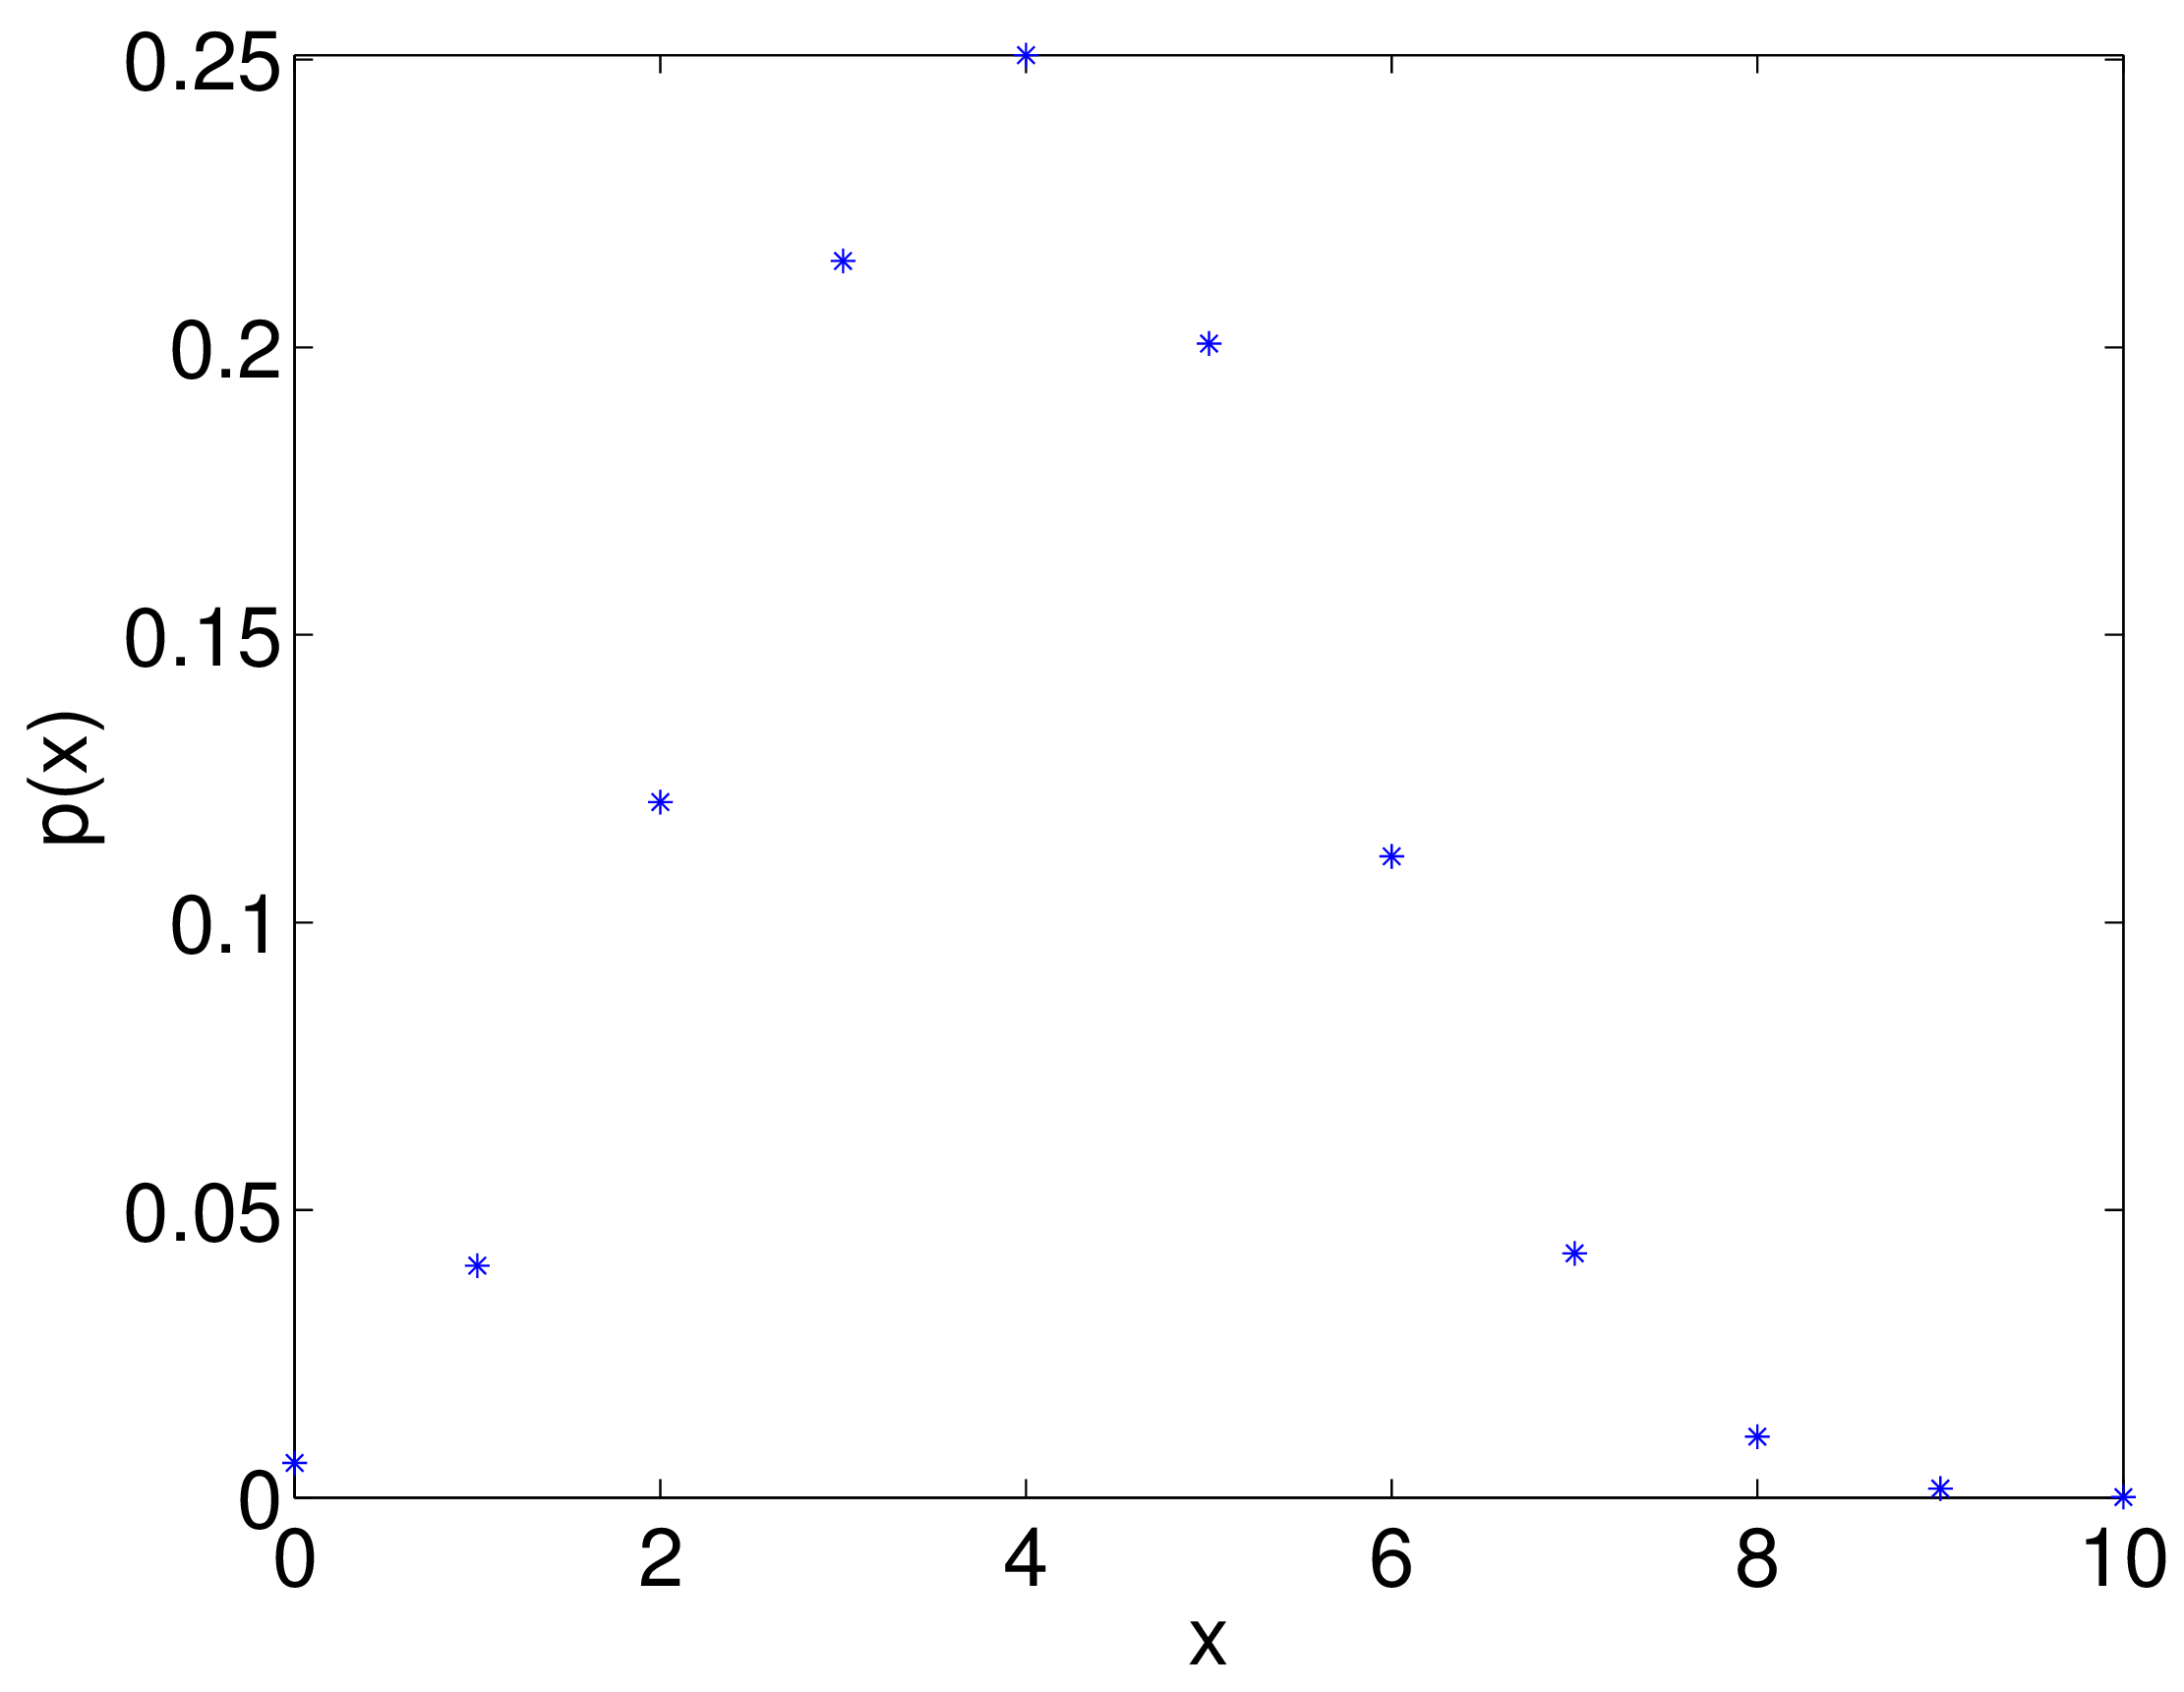
\includegraphics[scale=0.5]{vpbin2} }

\end{frame}

\begin{frame}[fragile]\frametitle{The binomial pdf}

\center{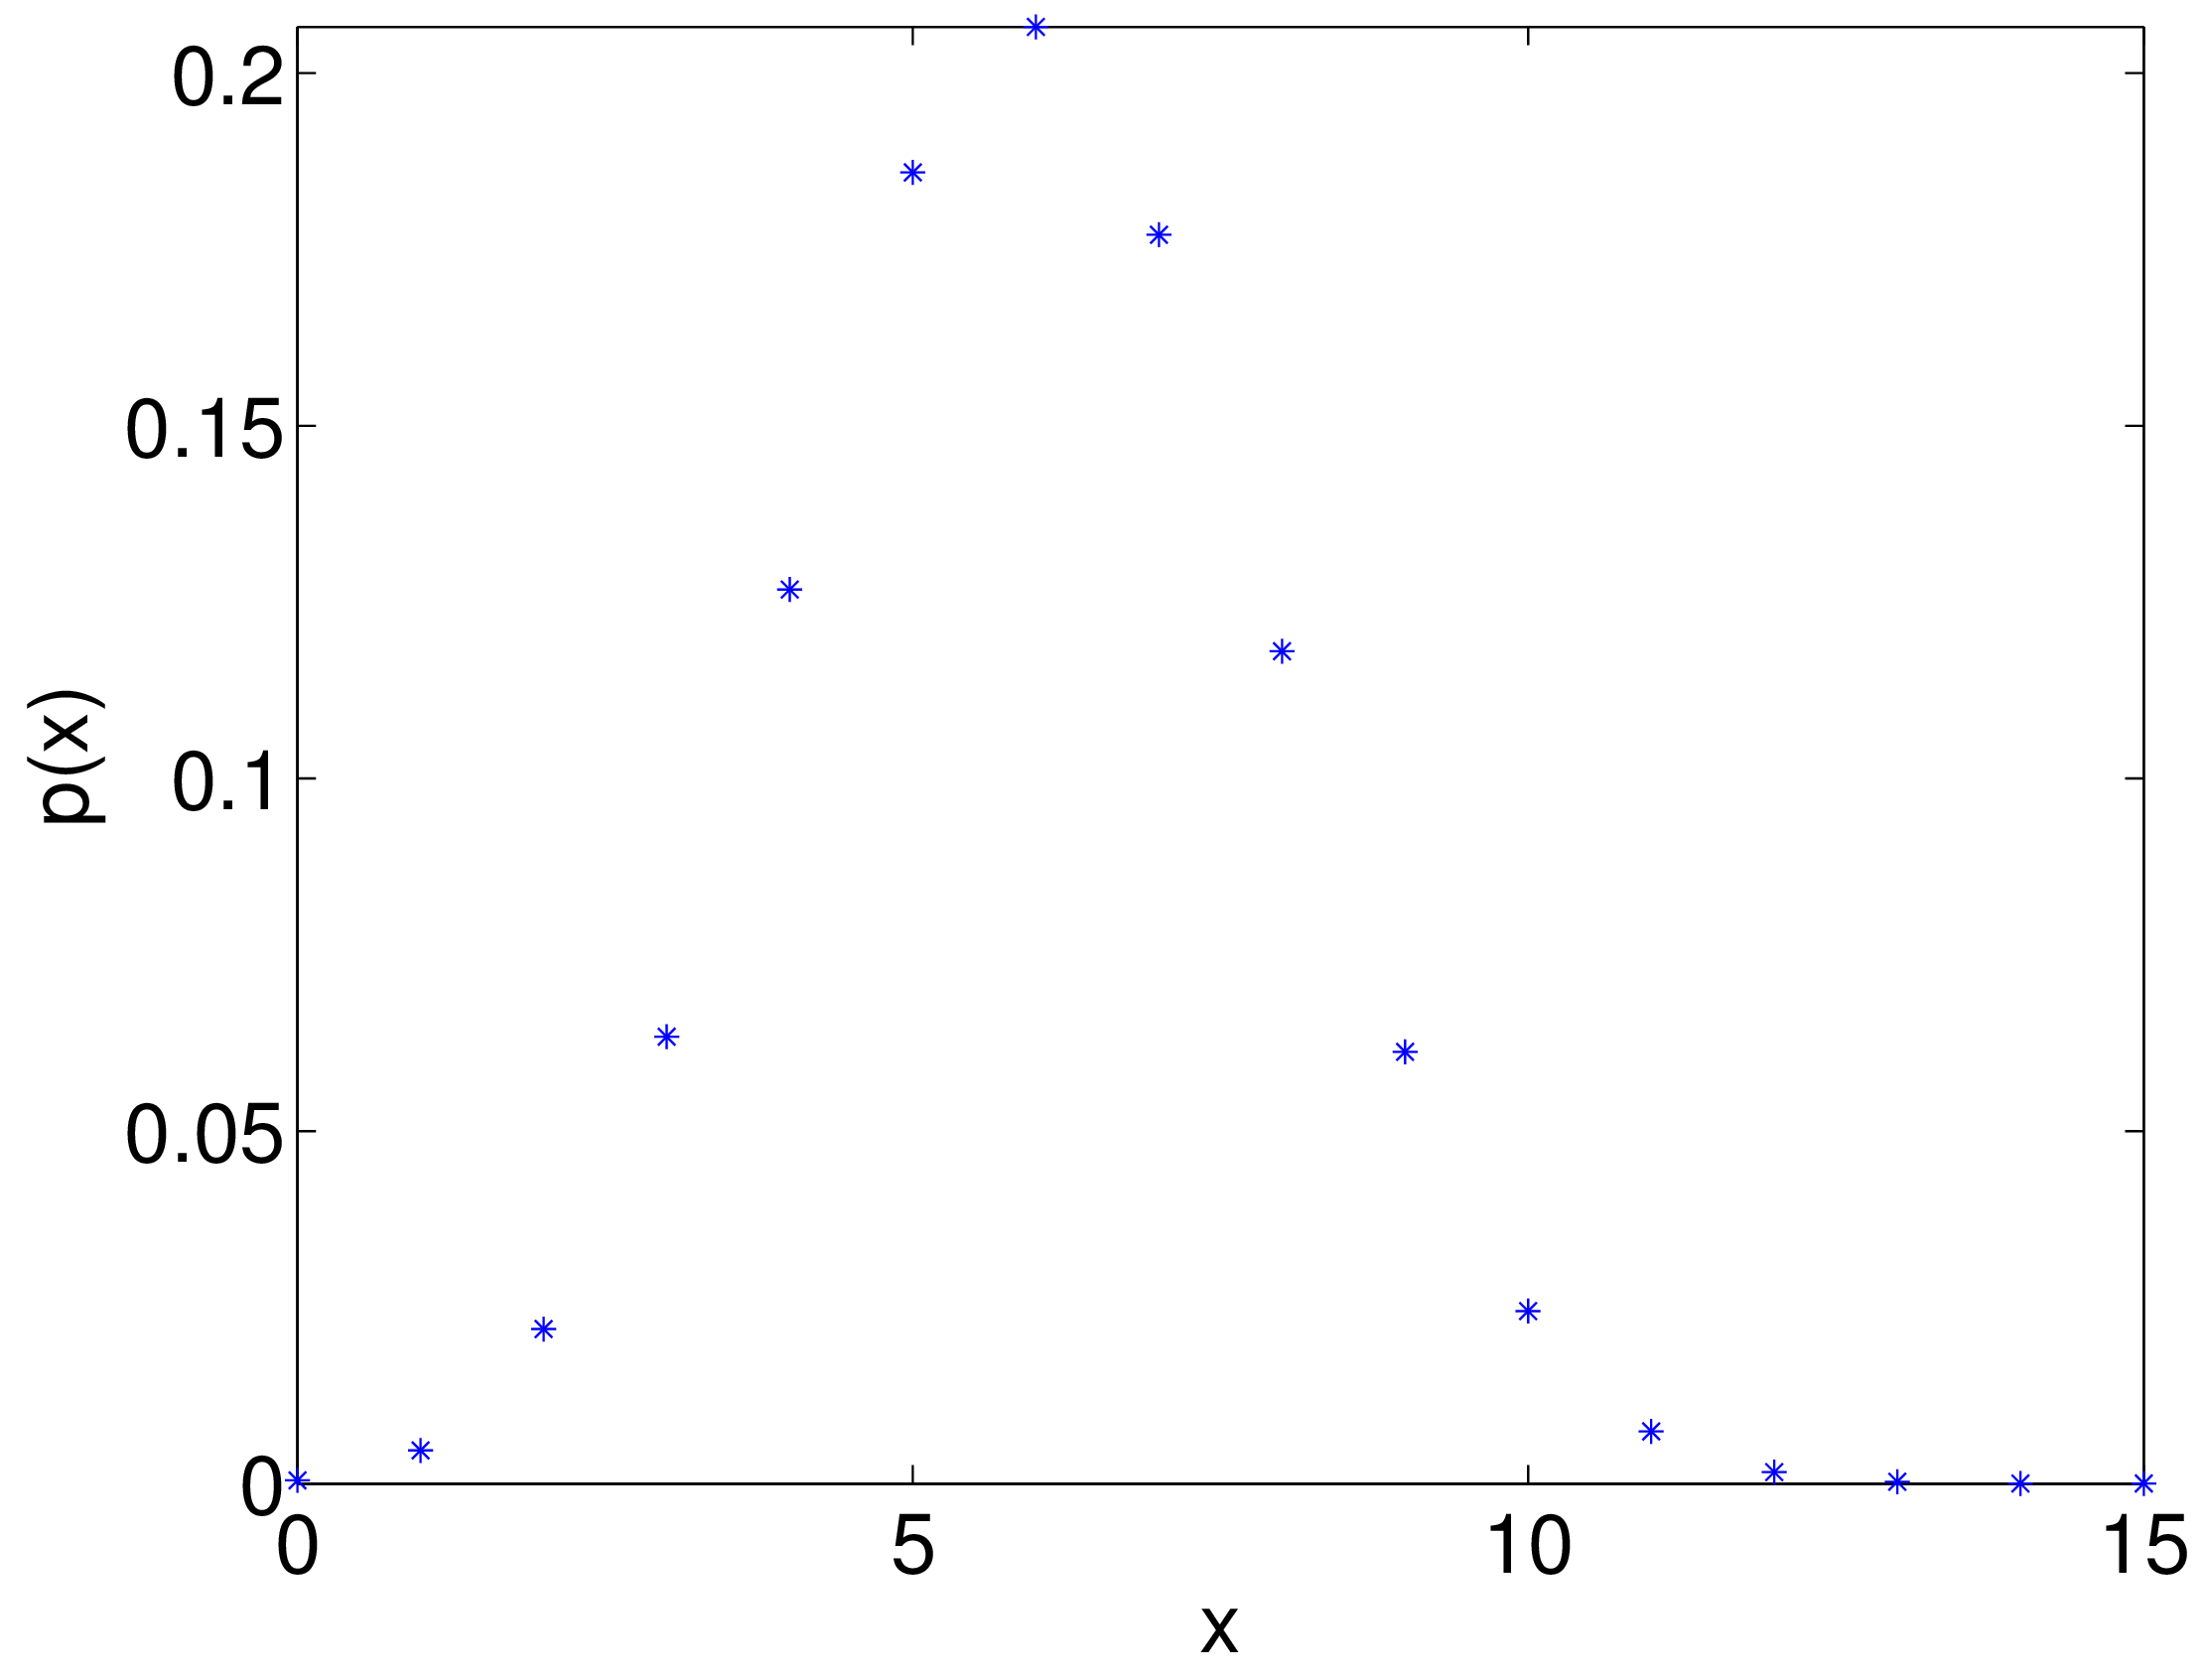
\includegraphics[scale=0.5]{vpbin3} }

\end{frame}

\begin{frame}[fragile]\frametitle{The binomial pdf}

\center{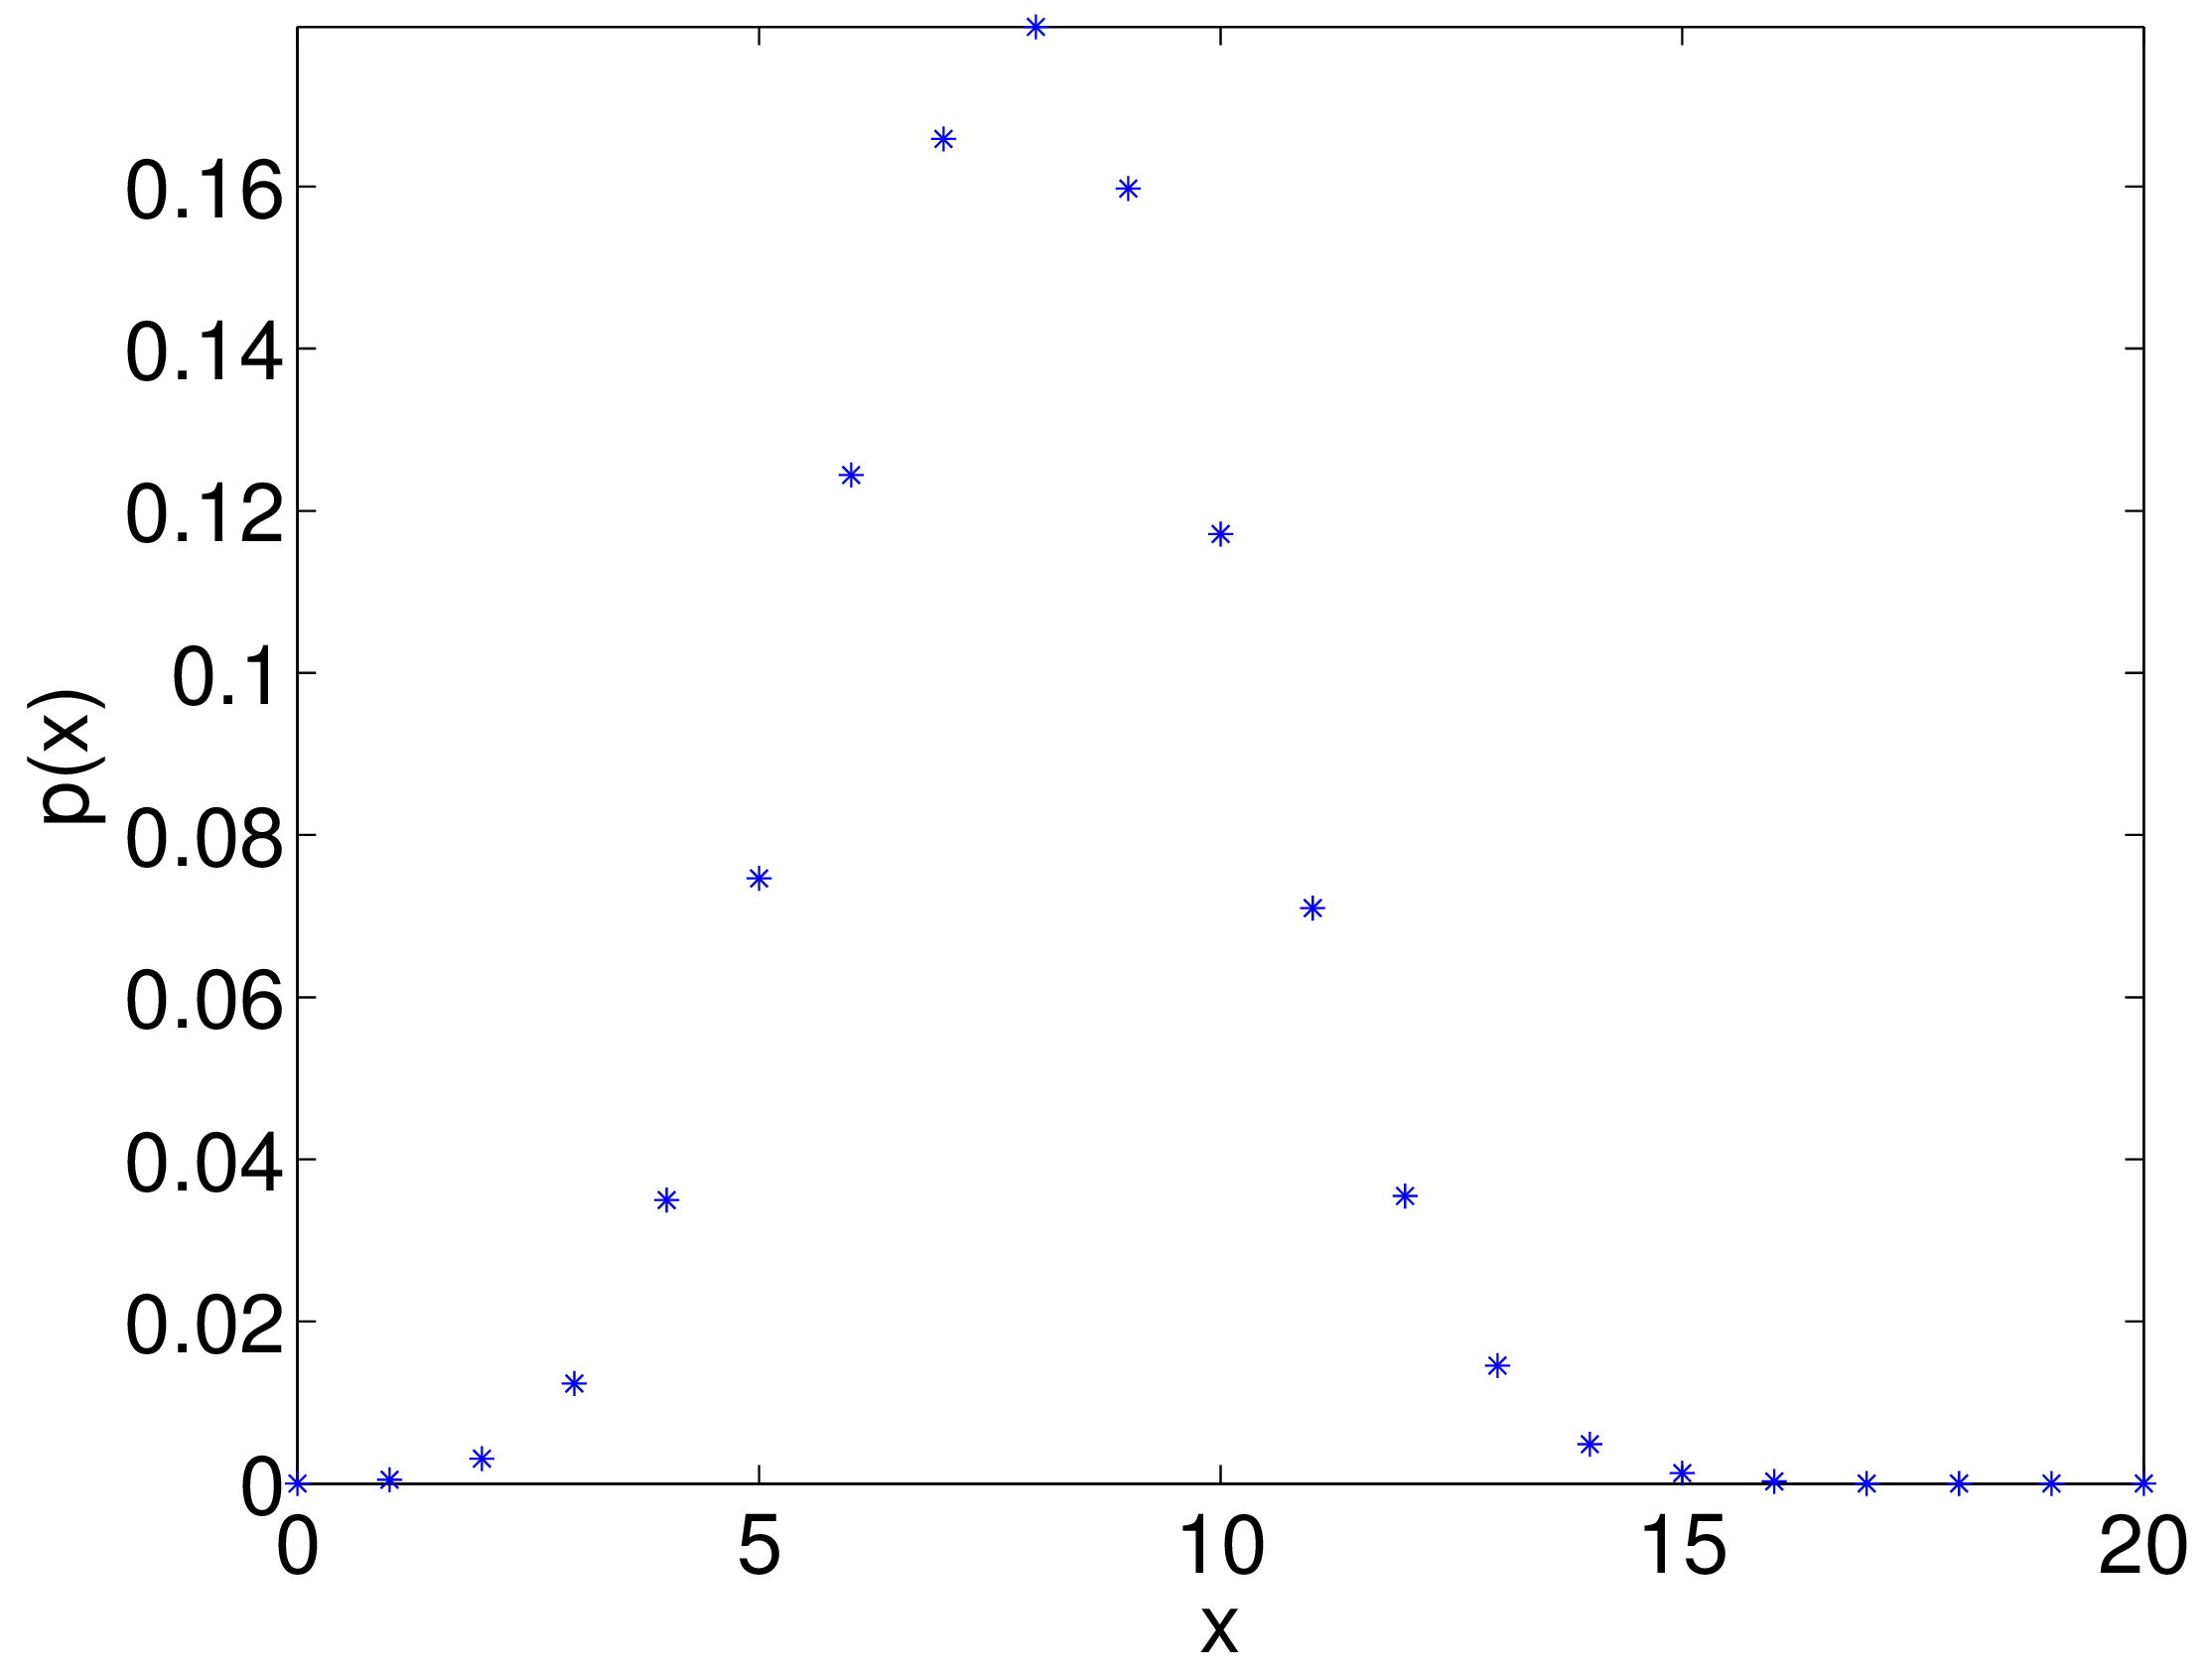
\includegraphics[scale=0.5]{vpbin4} }

\end{frame}

\begin{frame}[fragile]\frametitle{The binomial pdf}

\center{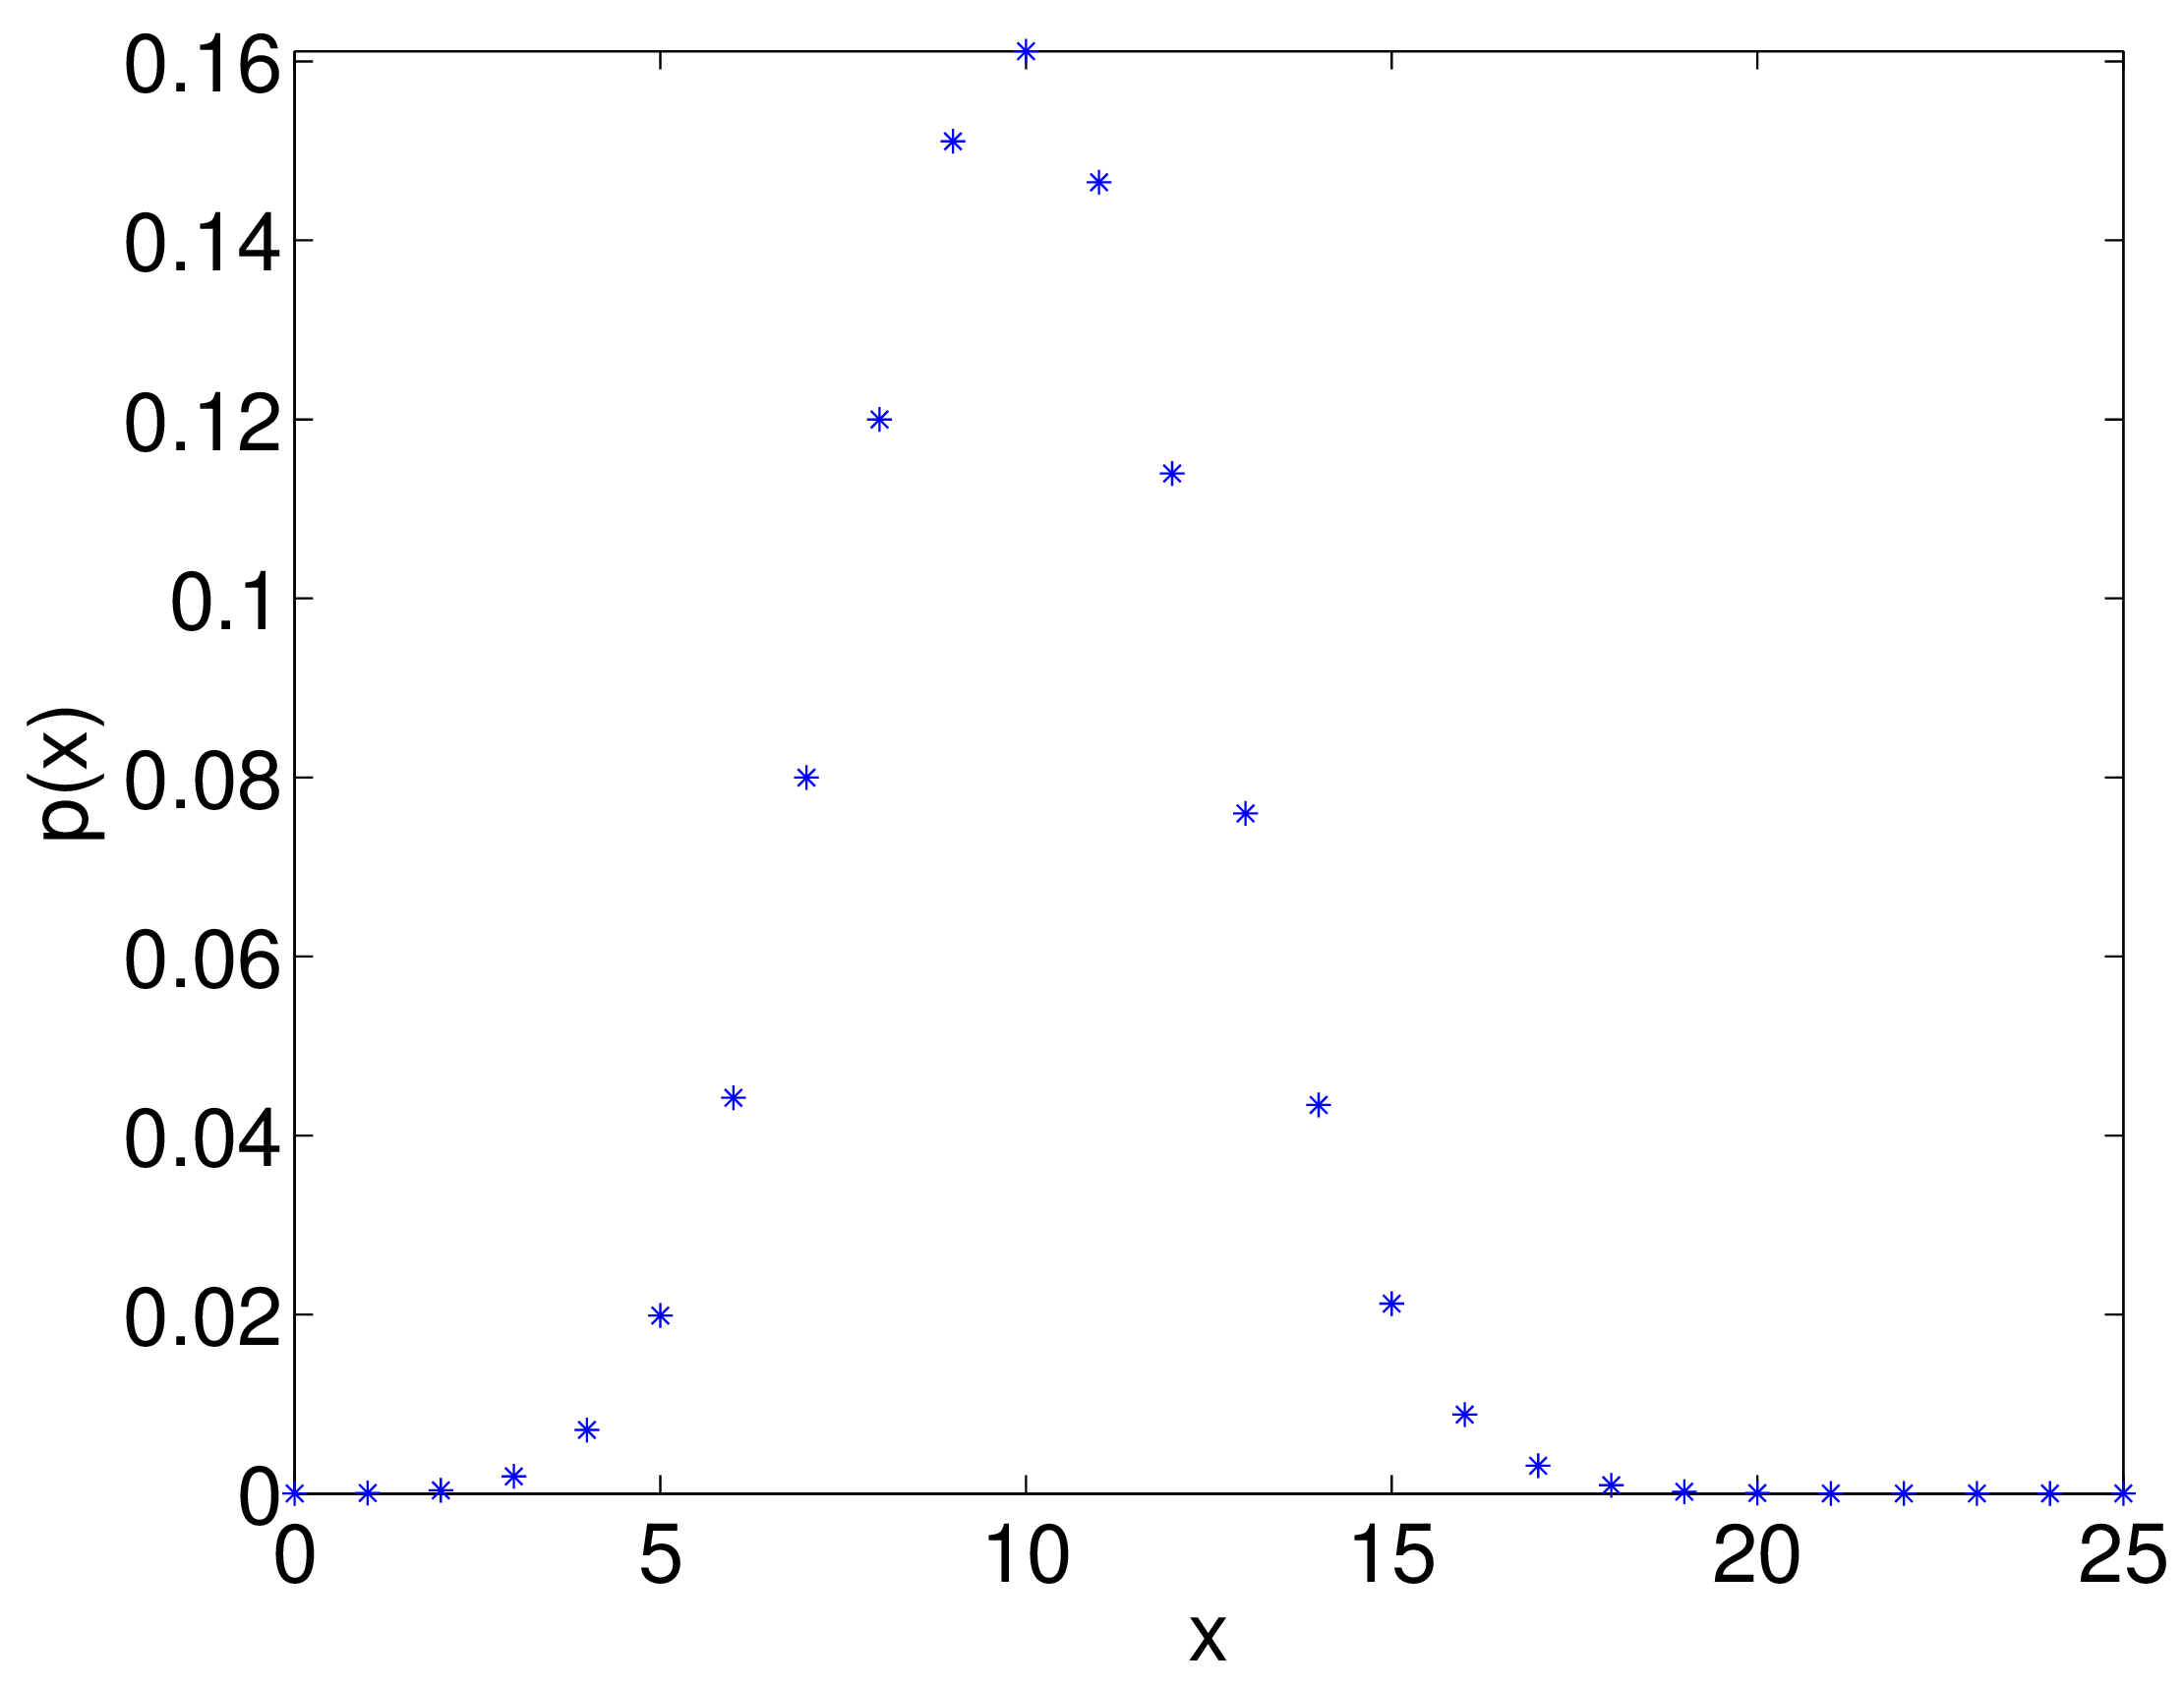
\includegraphics[scale=0.5]{vpbin5} }
\end{frame}

\begin{frame}[fragile]\frametitle{The binomial pdf}

\center{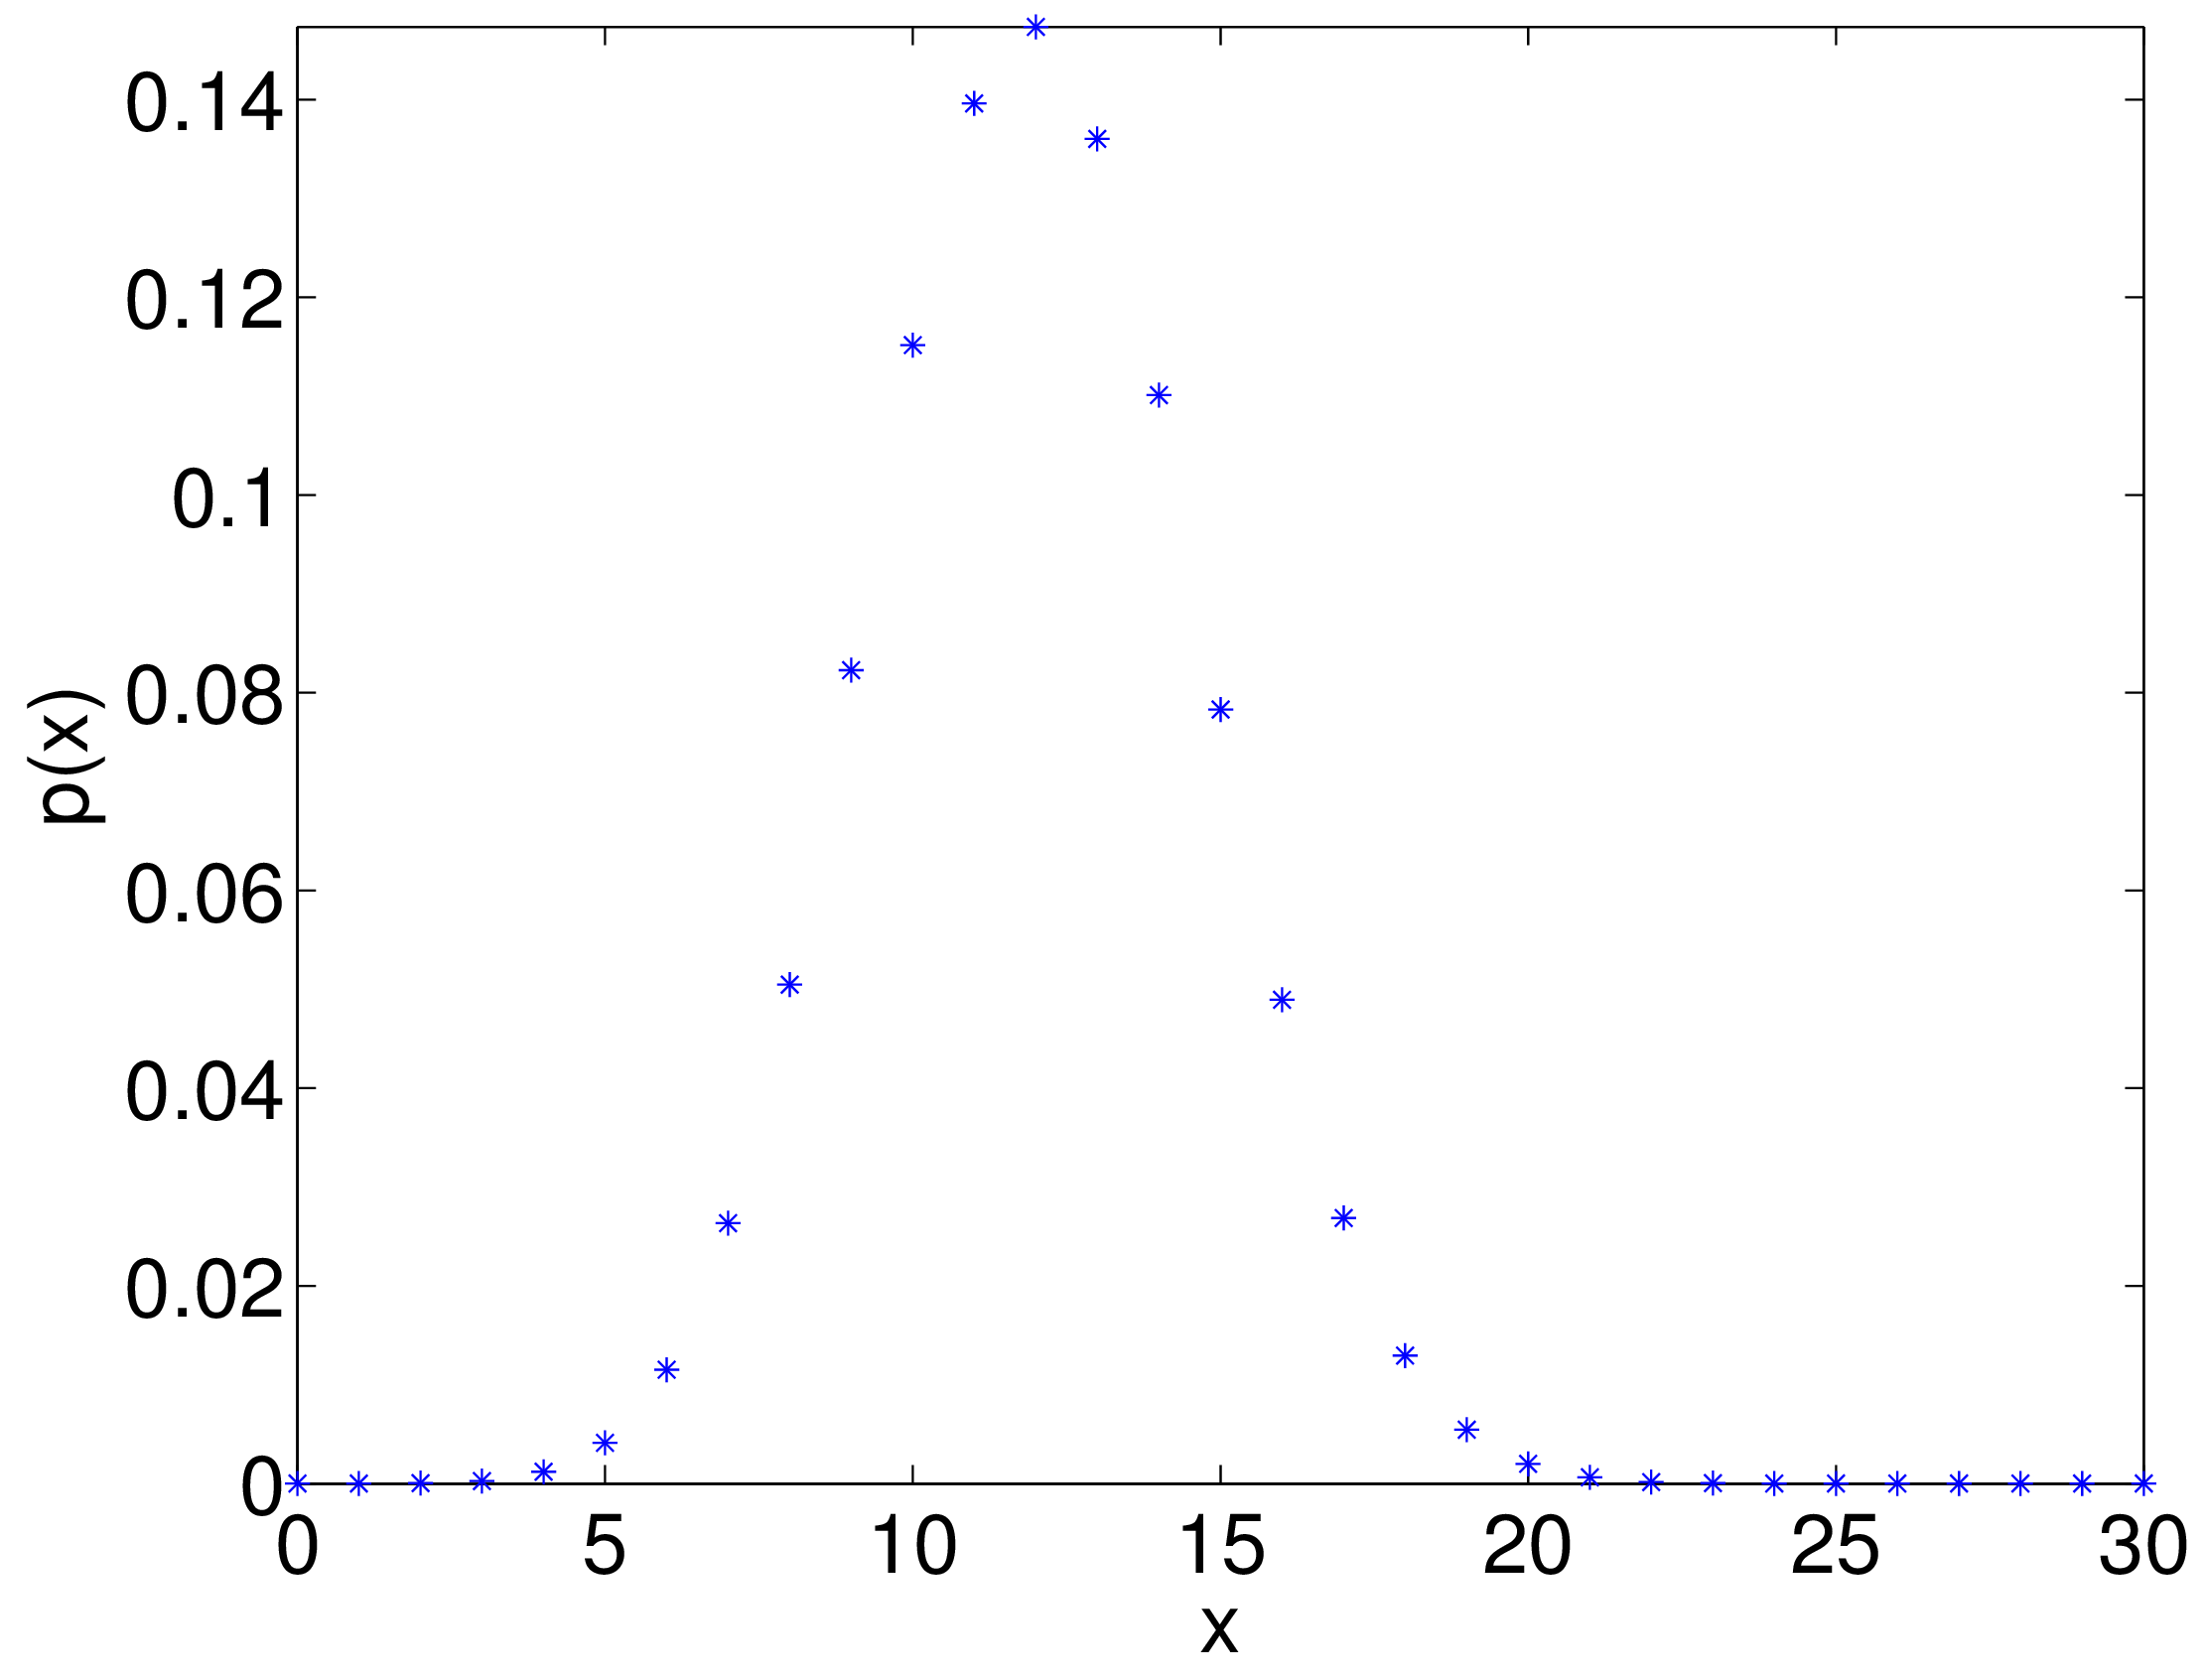
\includegraphics[scale=0.5]{vpbin6} }

\end{frame}

\begin{frame}[fragile]\frametitle{The binomial pdf}

\center{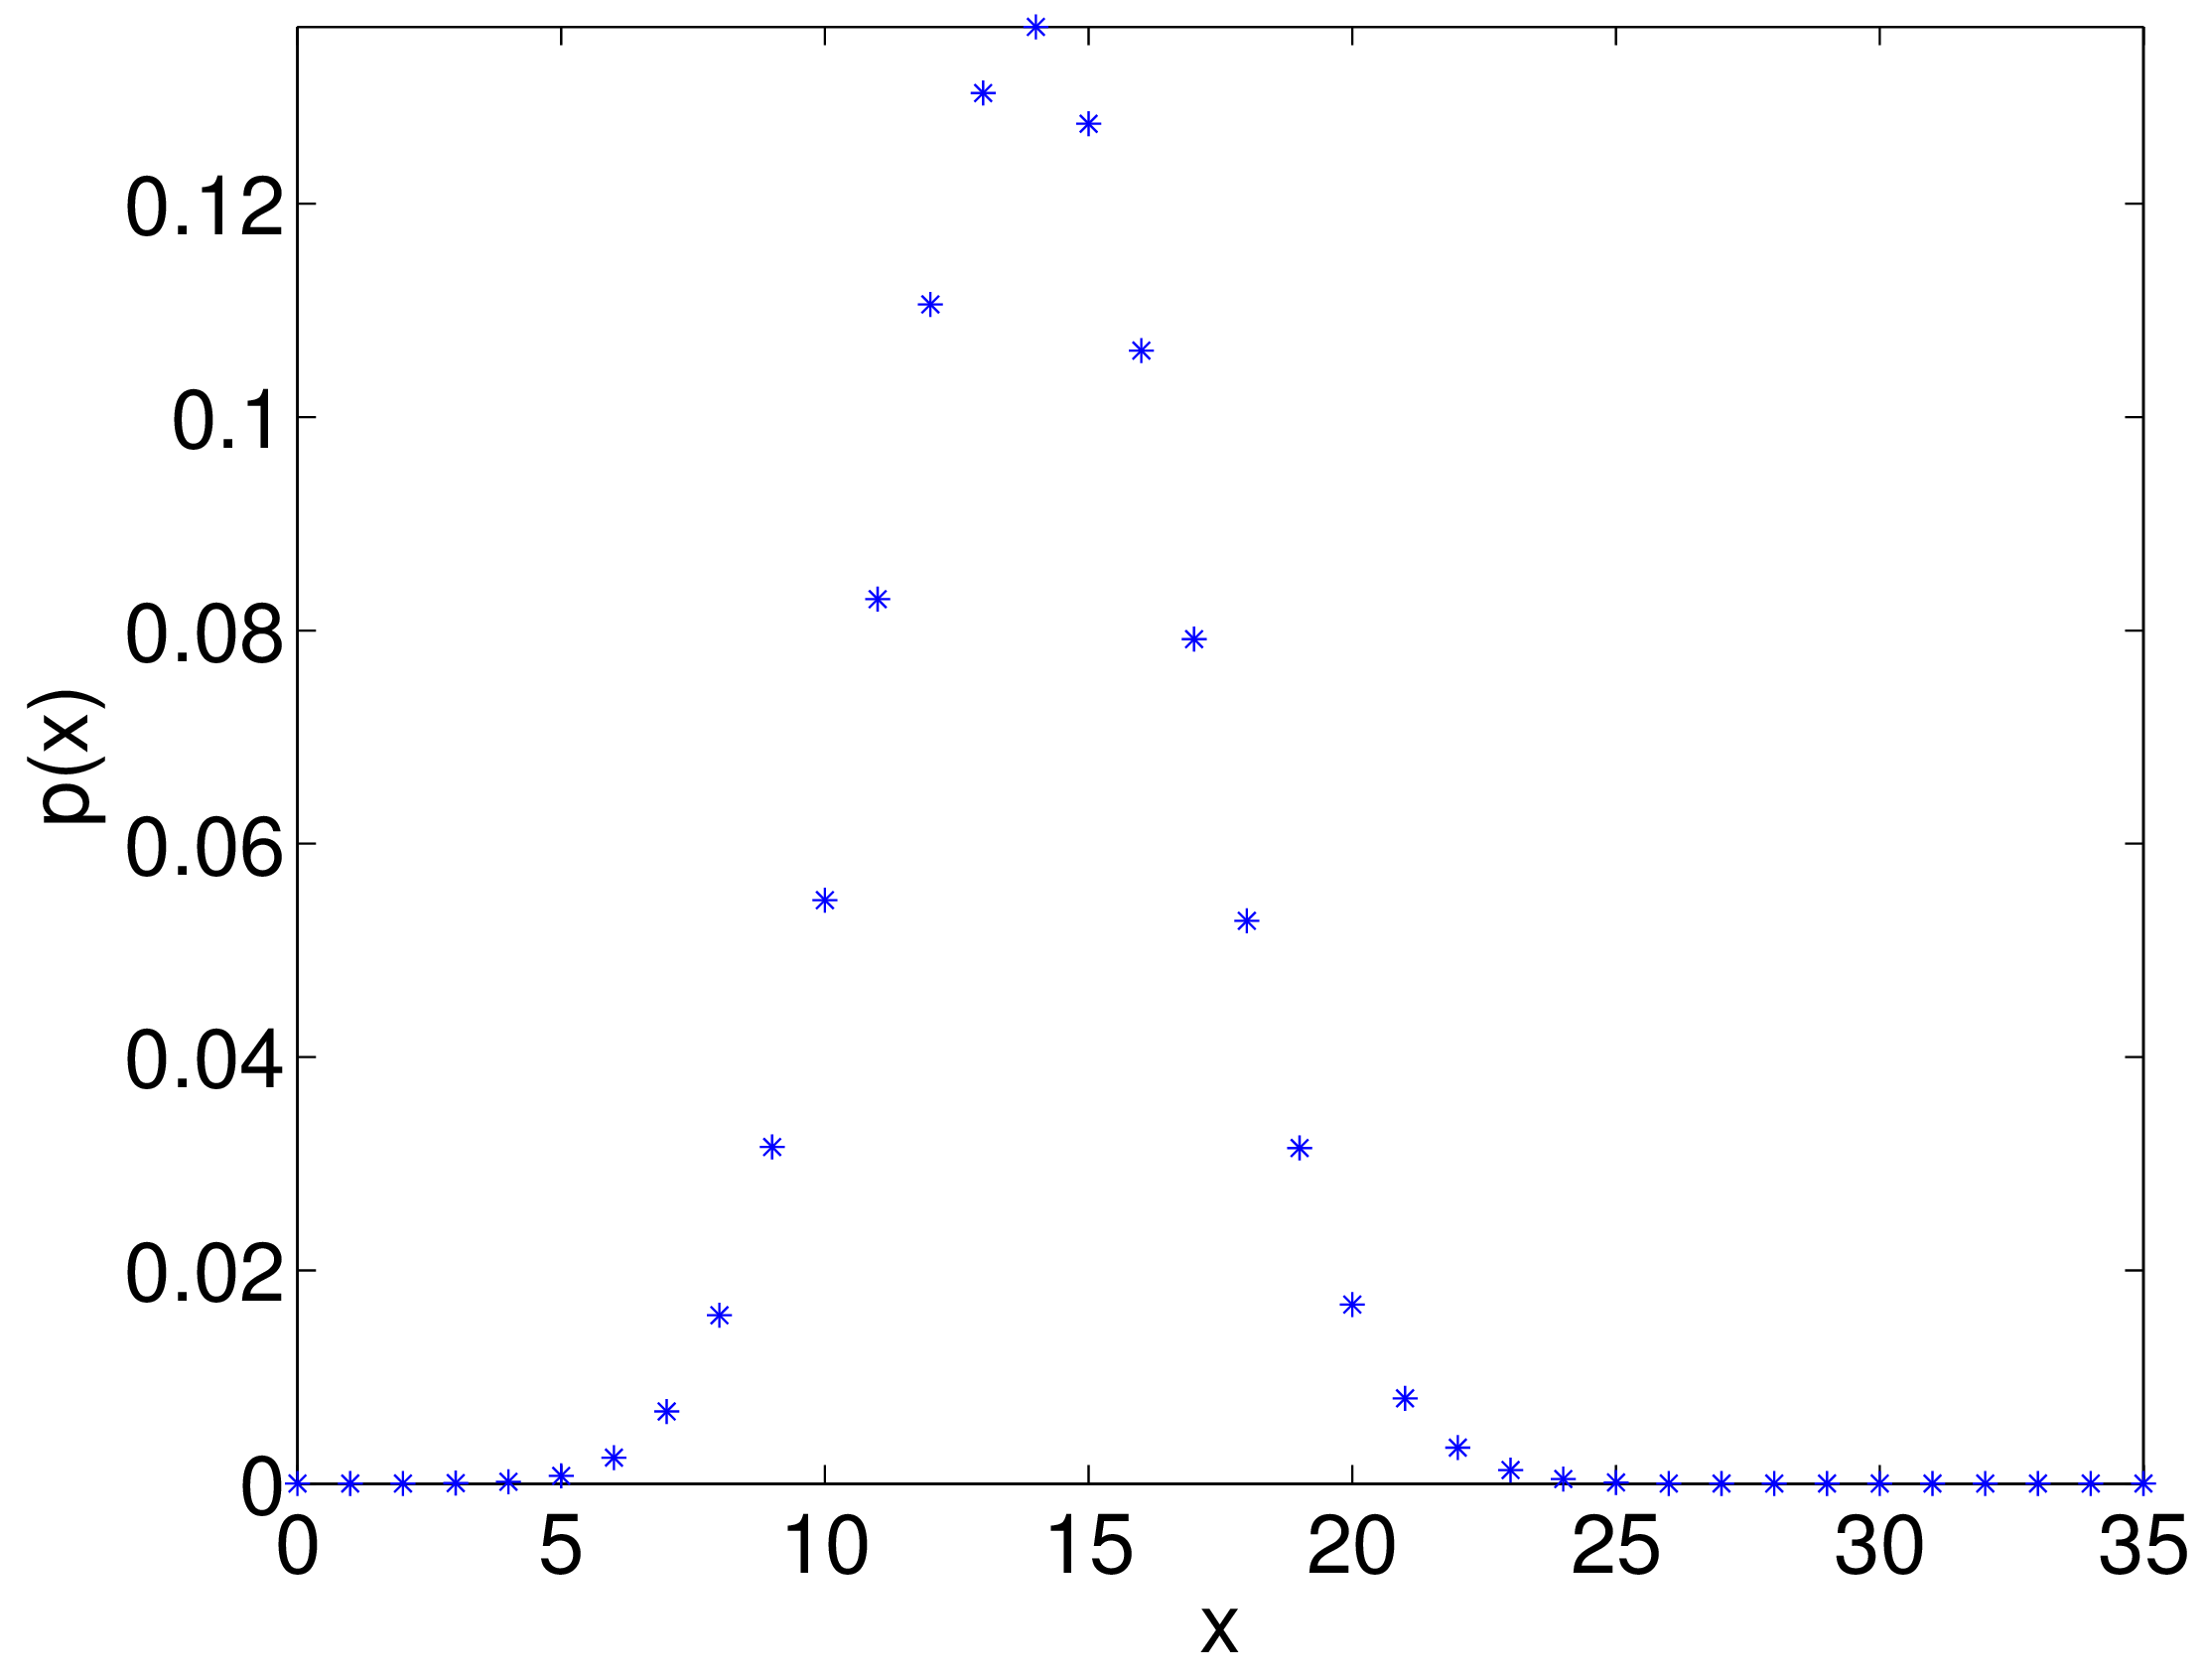
\includegraphics[scale=0.5]{vpbin7} }

\end{frame}

\begin{frame}[fragile]\frametitle{The binomial pdf}

\center{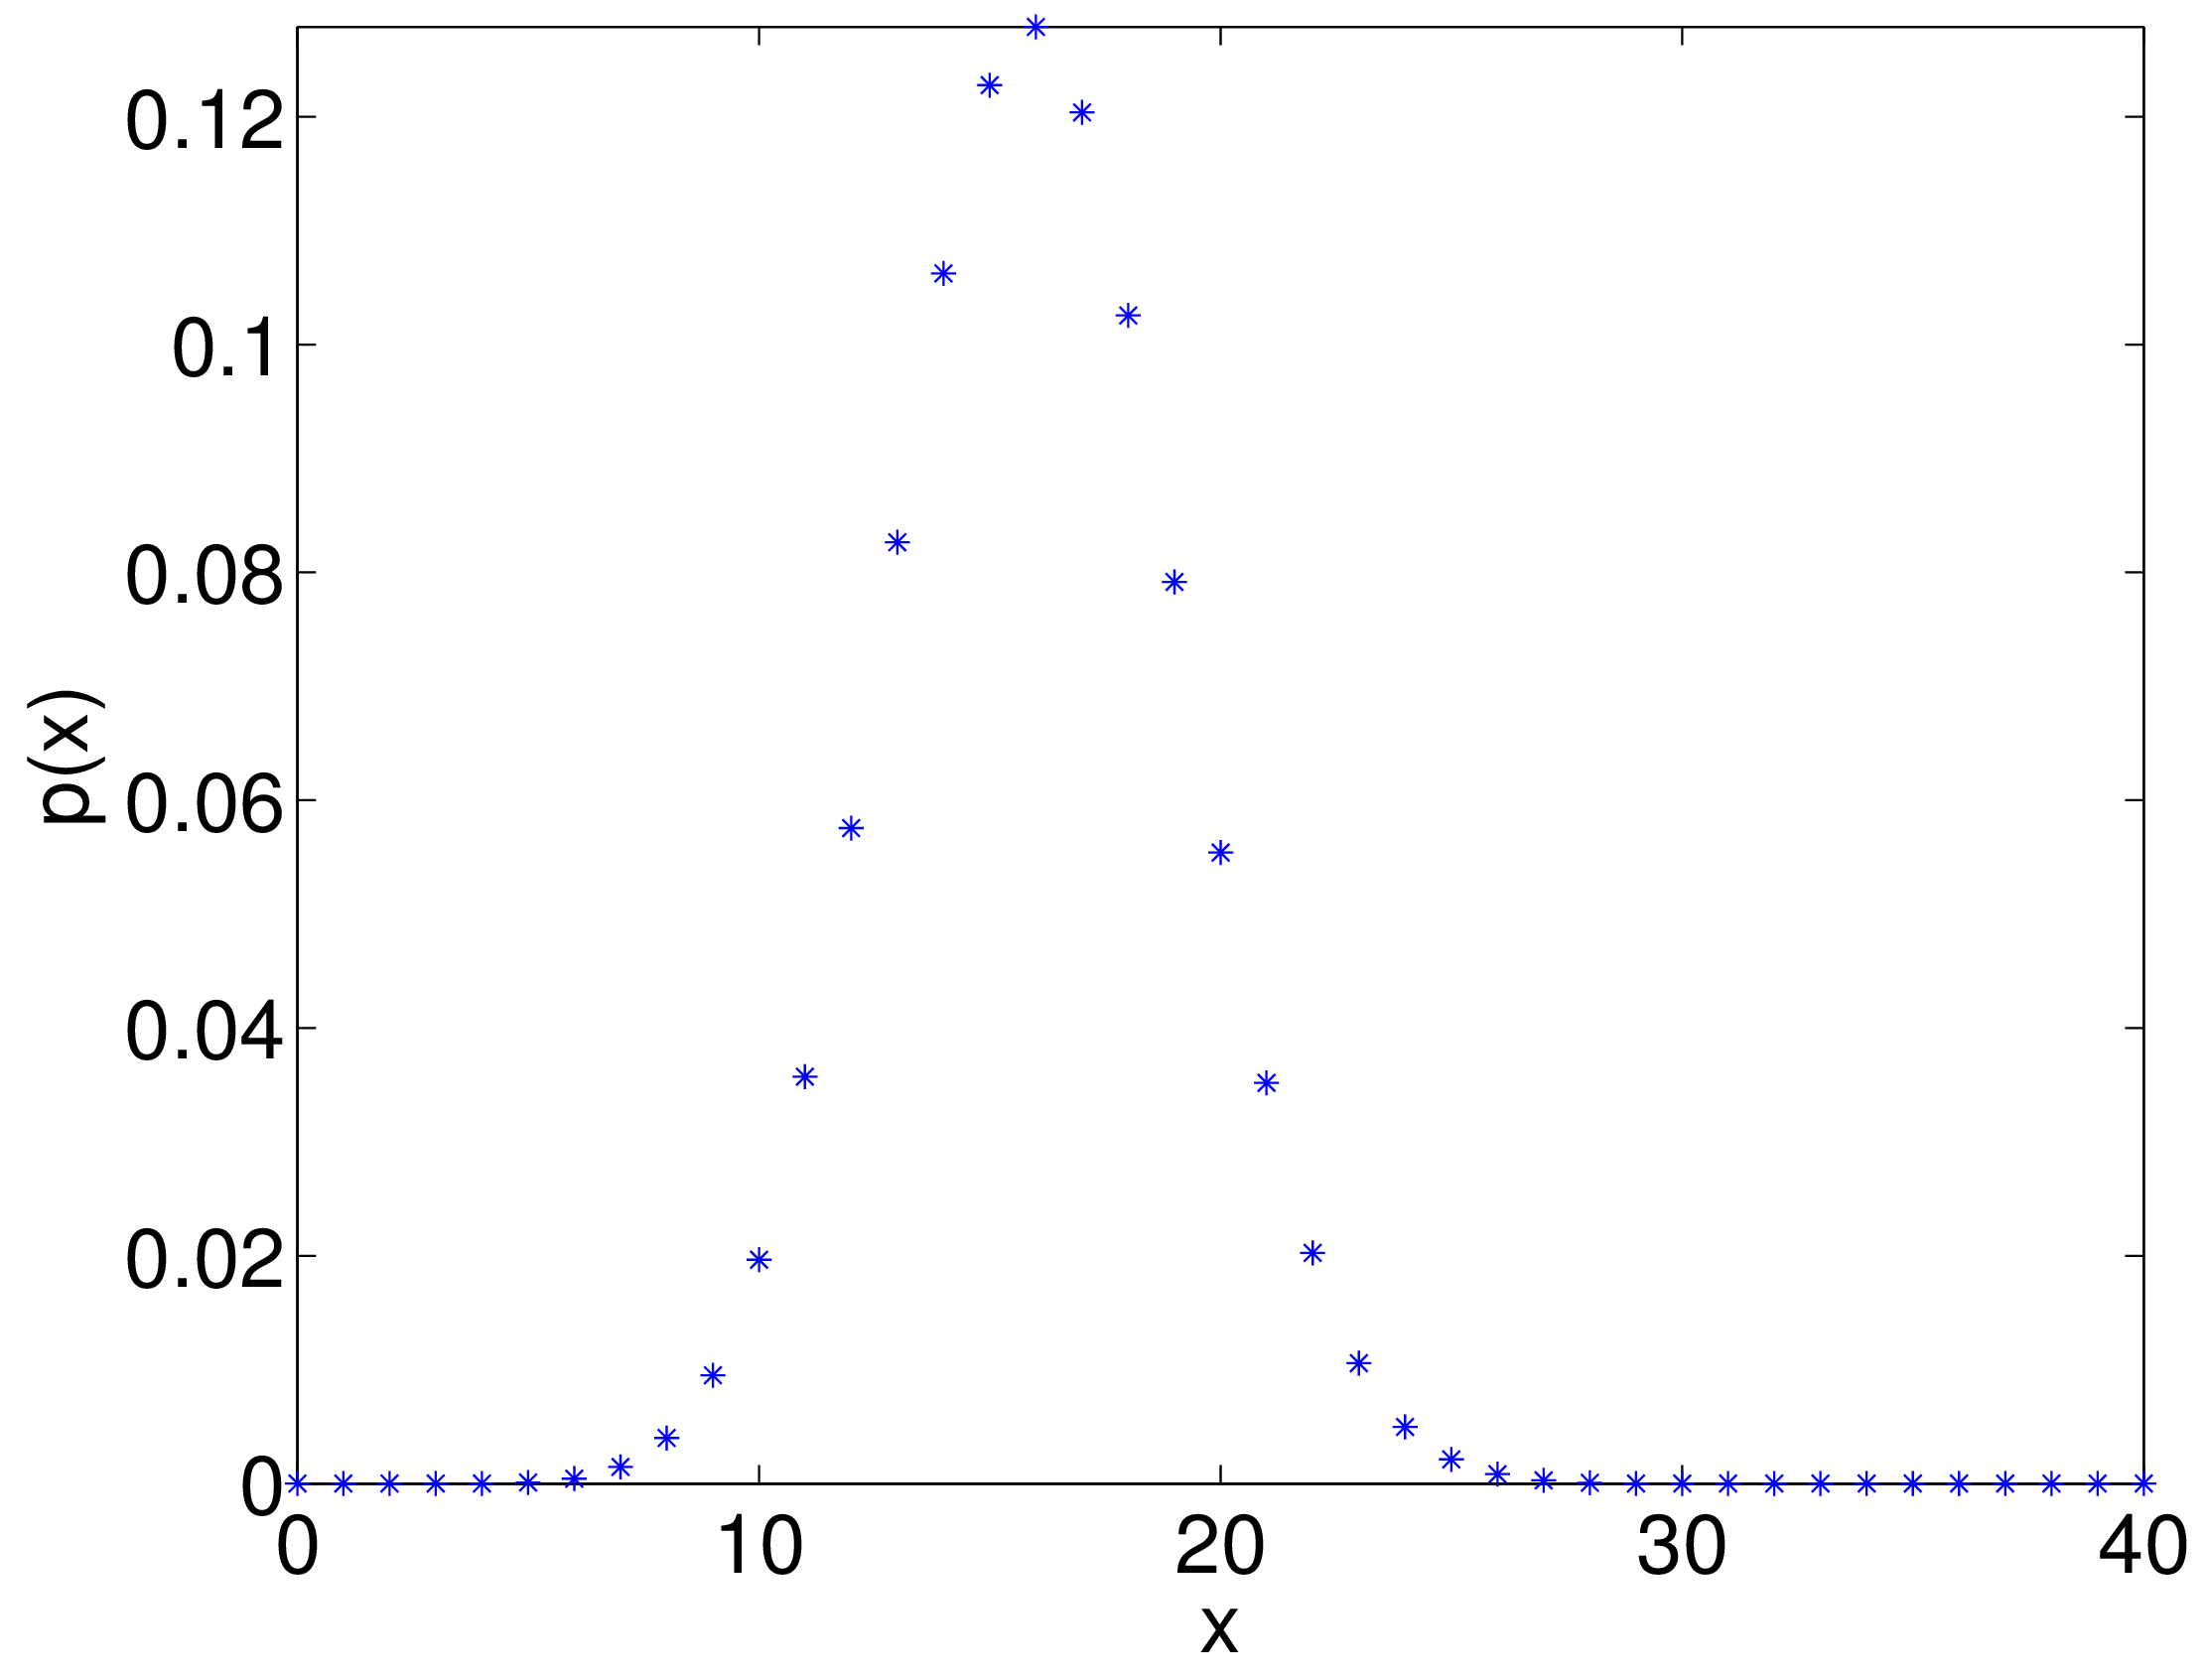
\includegraphics[scale=0.5]{vpbin8} }

\end{frame}

\begin{frame}[fragile]\frametitle{The binomial pdf}

\center{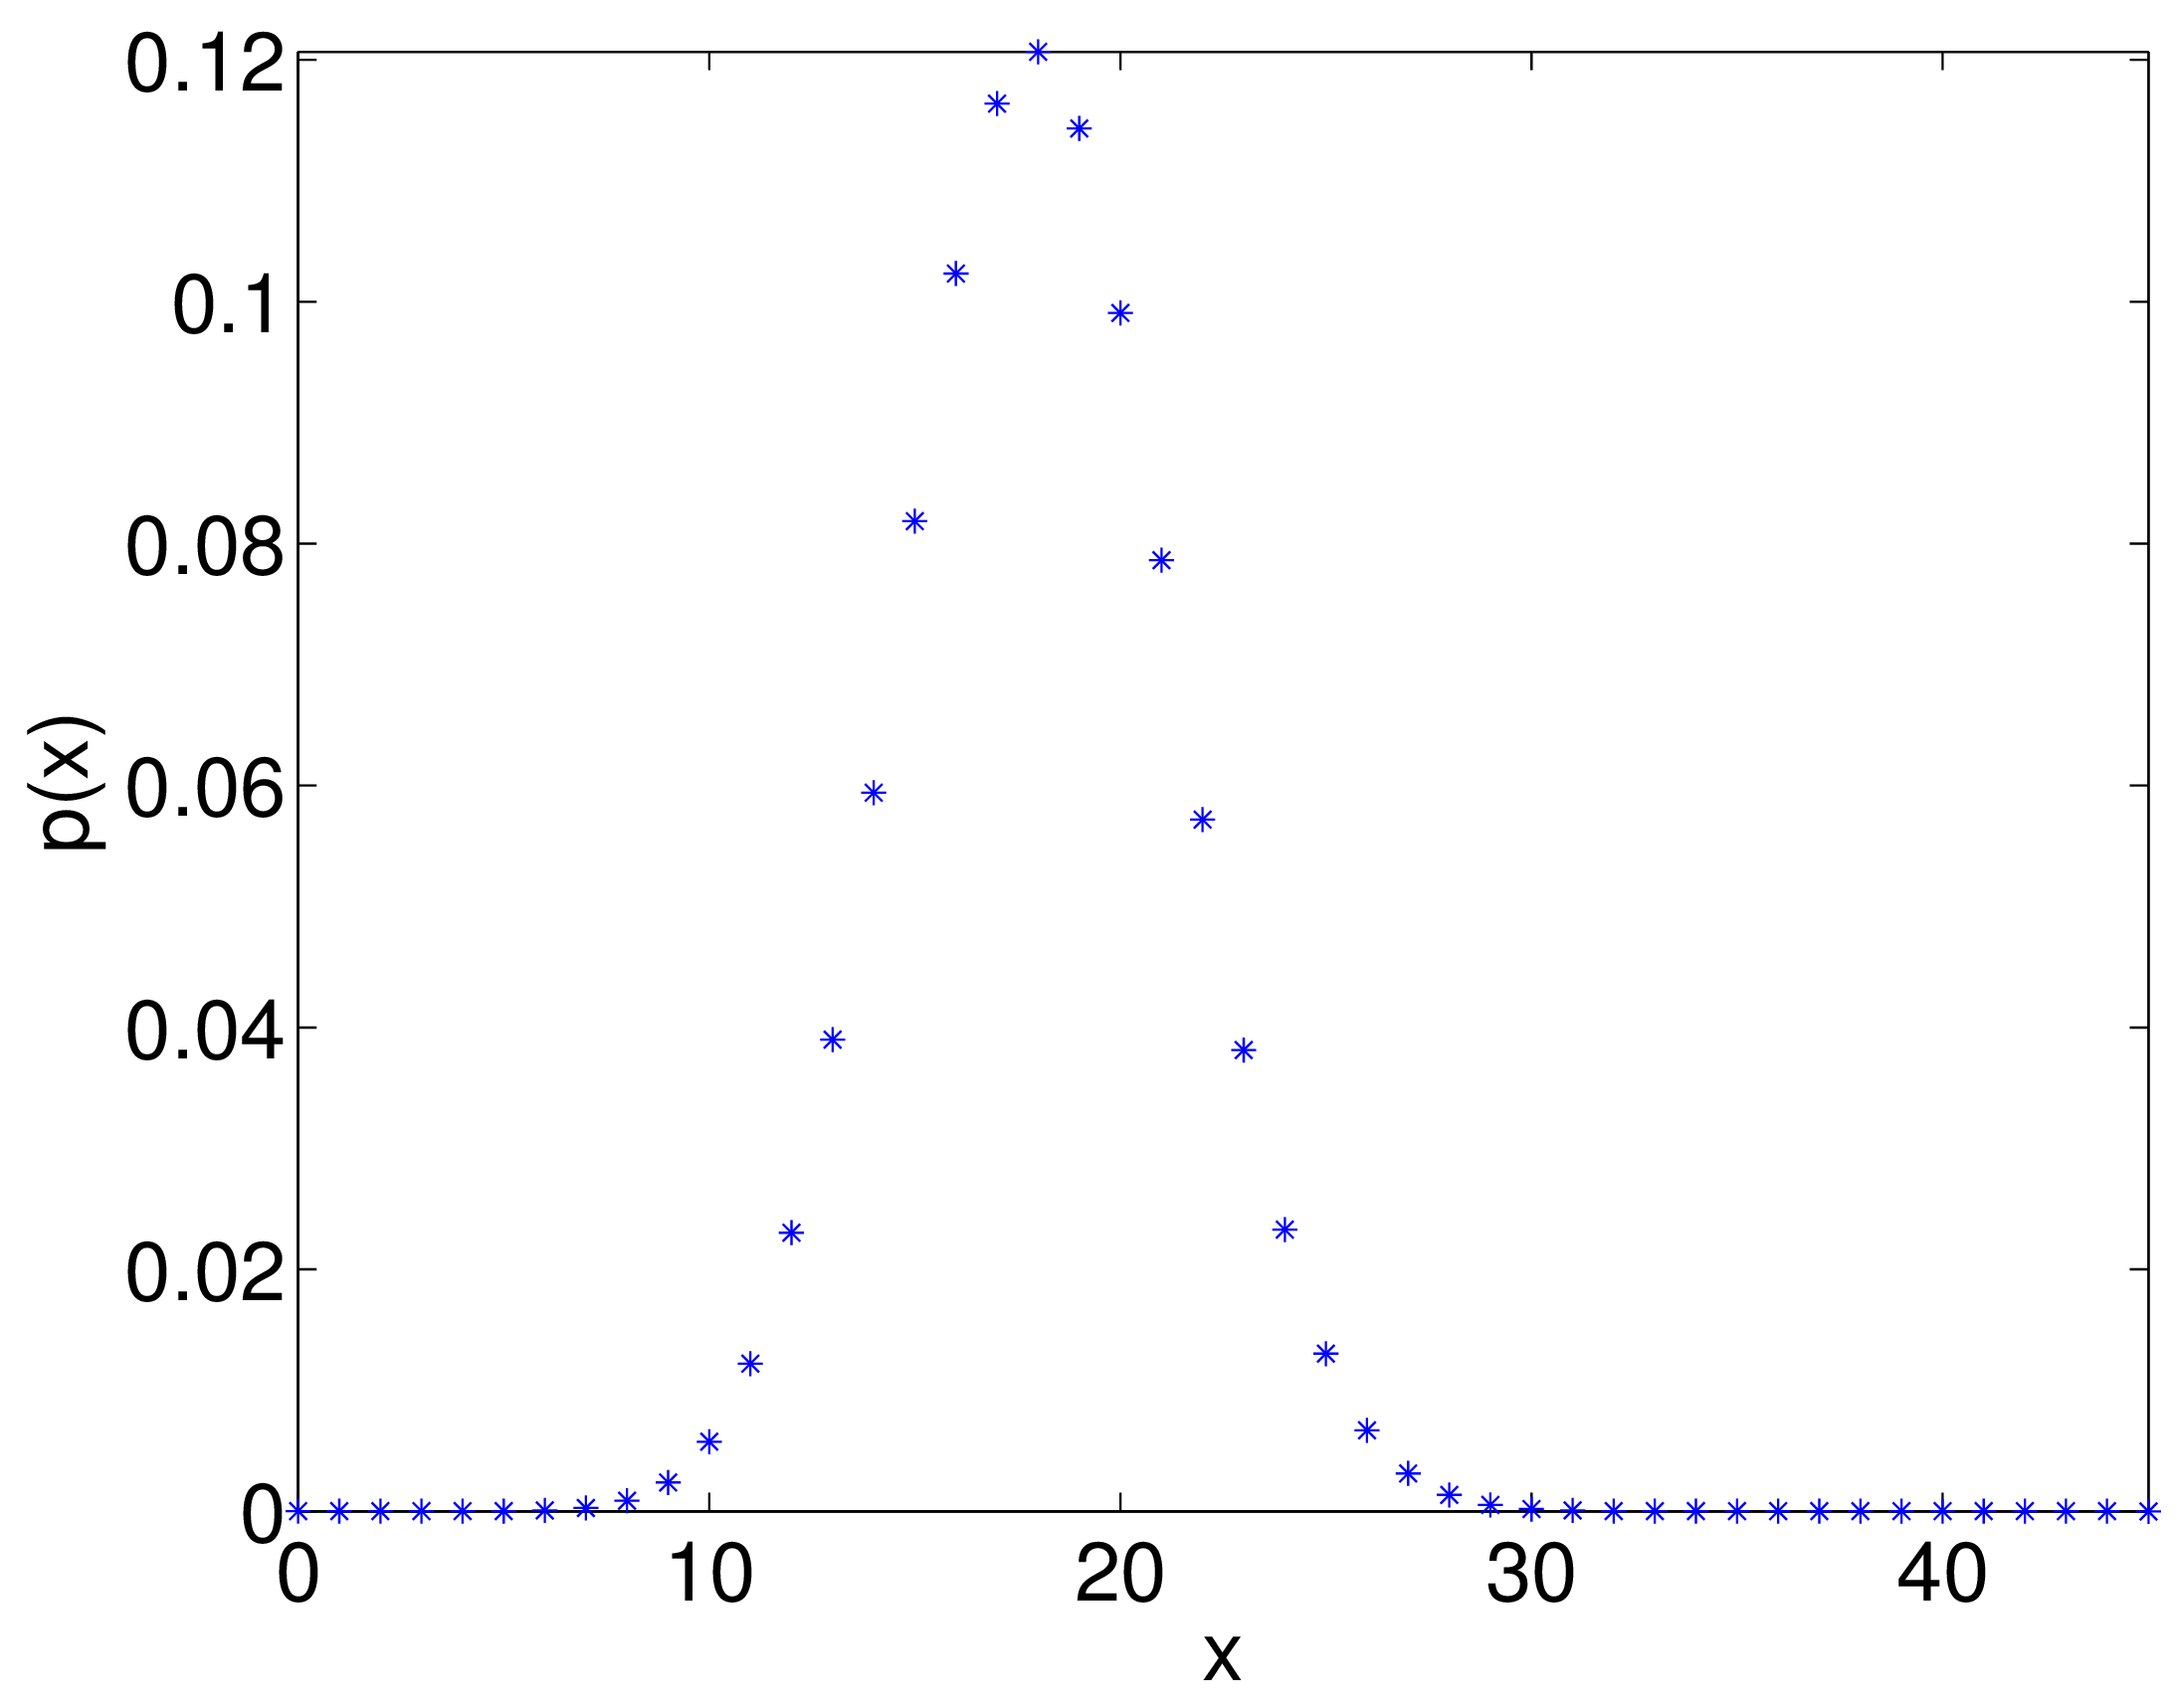
\includegraphics[scale=0.5]{vpbin9} }

\end{frame}

\begin{frame}[fragile]\frametitle{The binomial pdf}

\center{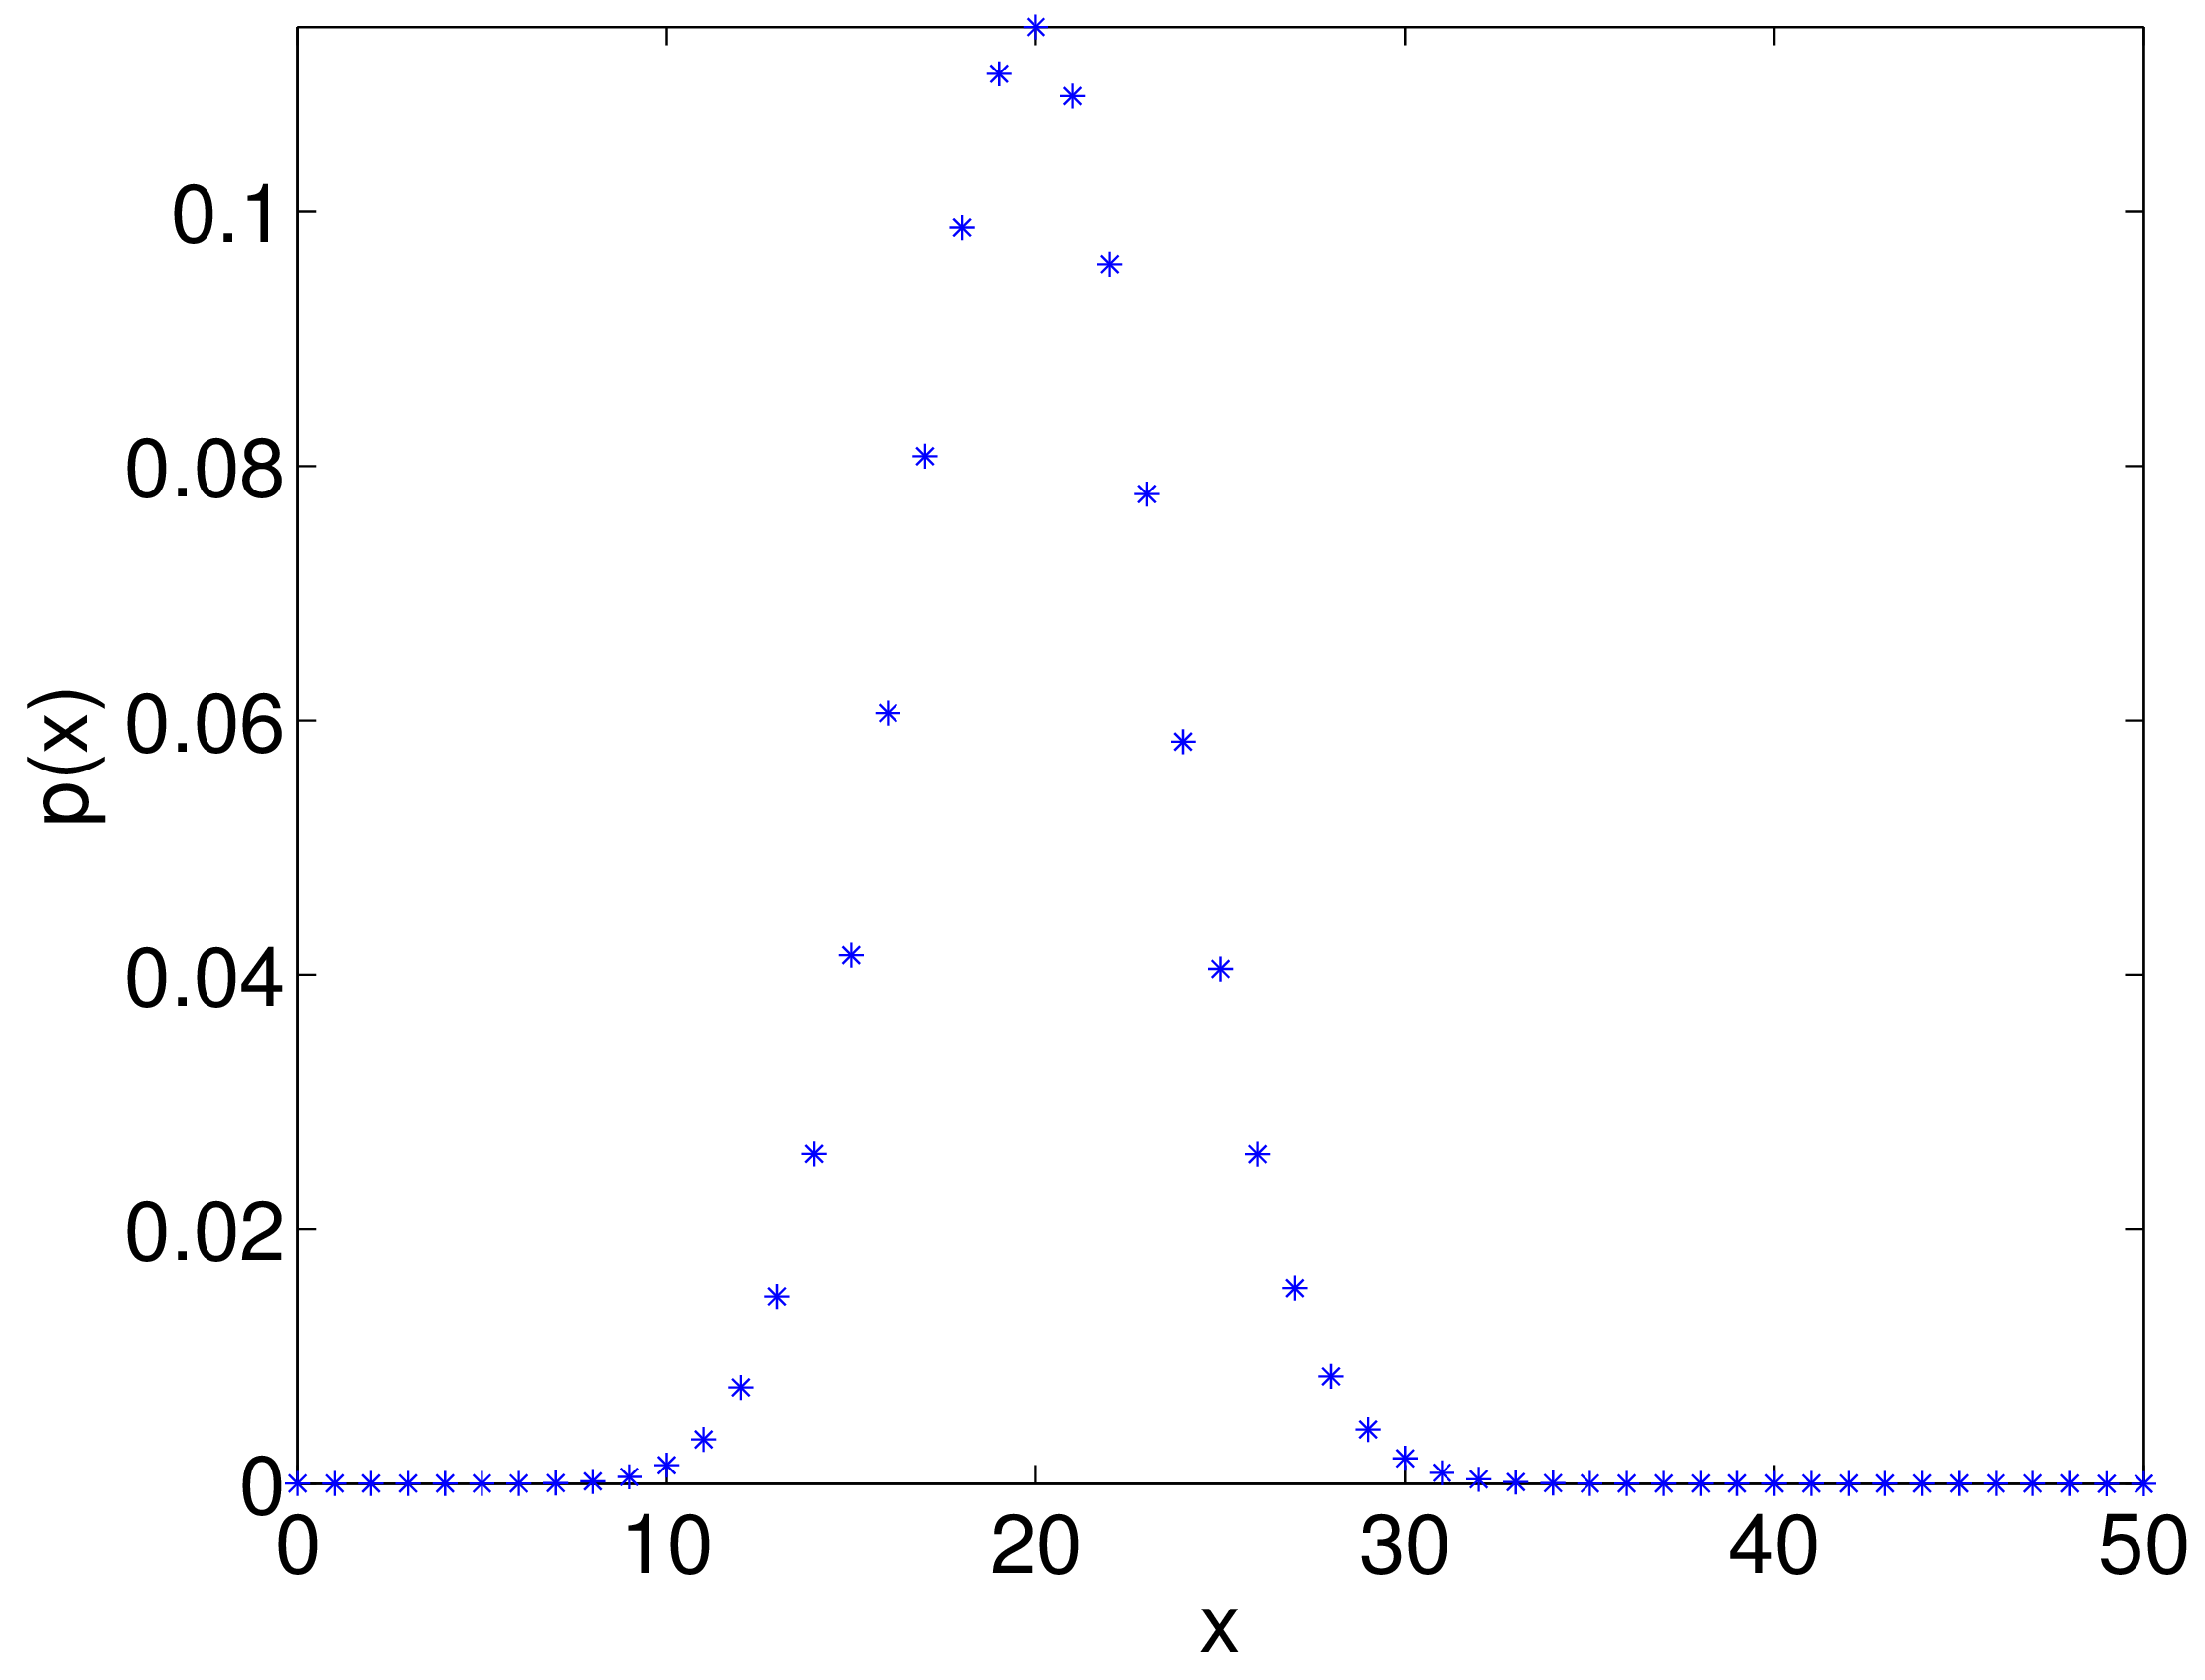
\includegraphics[scale=0.5]{vpbin10} }

\end{frame}

\begin{frame}[fragile]\frametitle{The binomial pdf}

\center{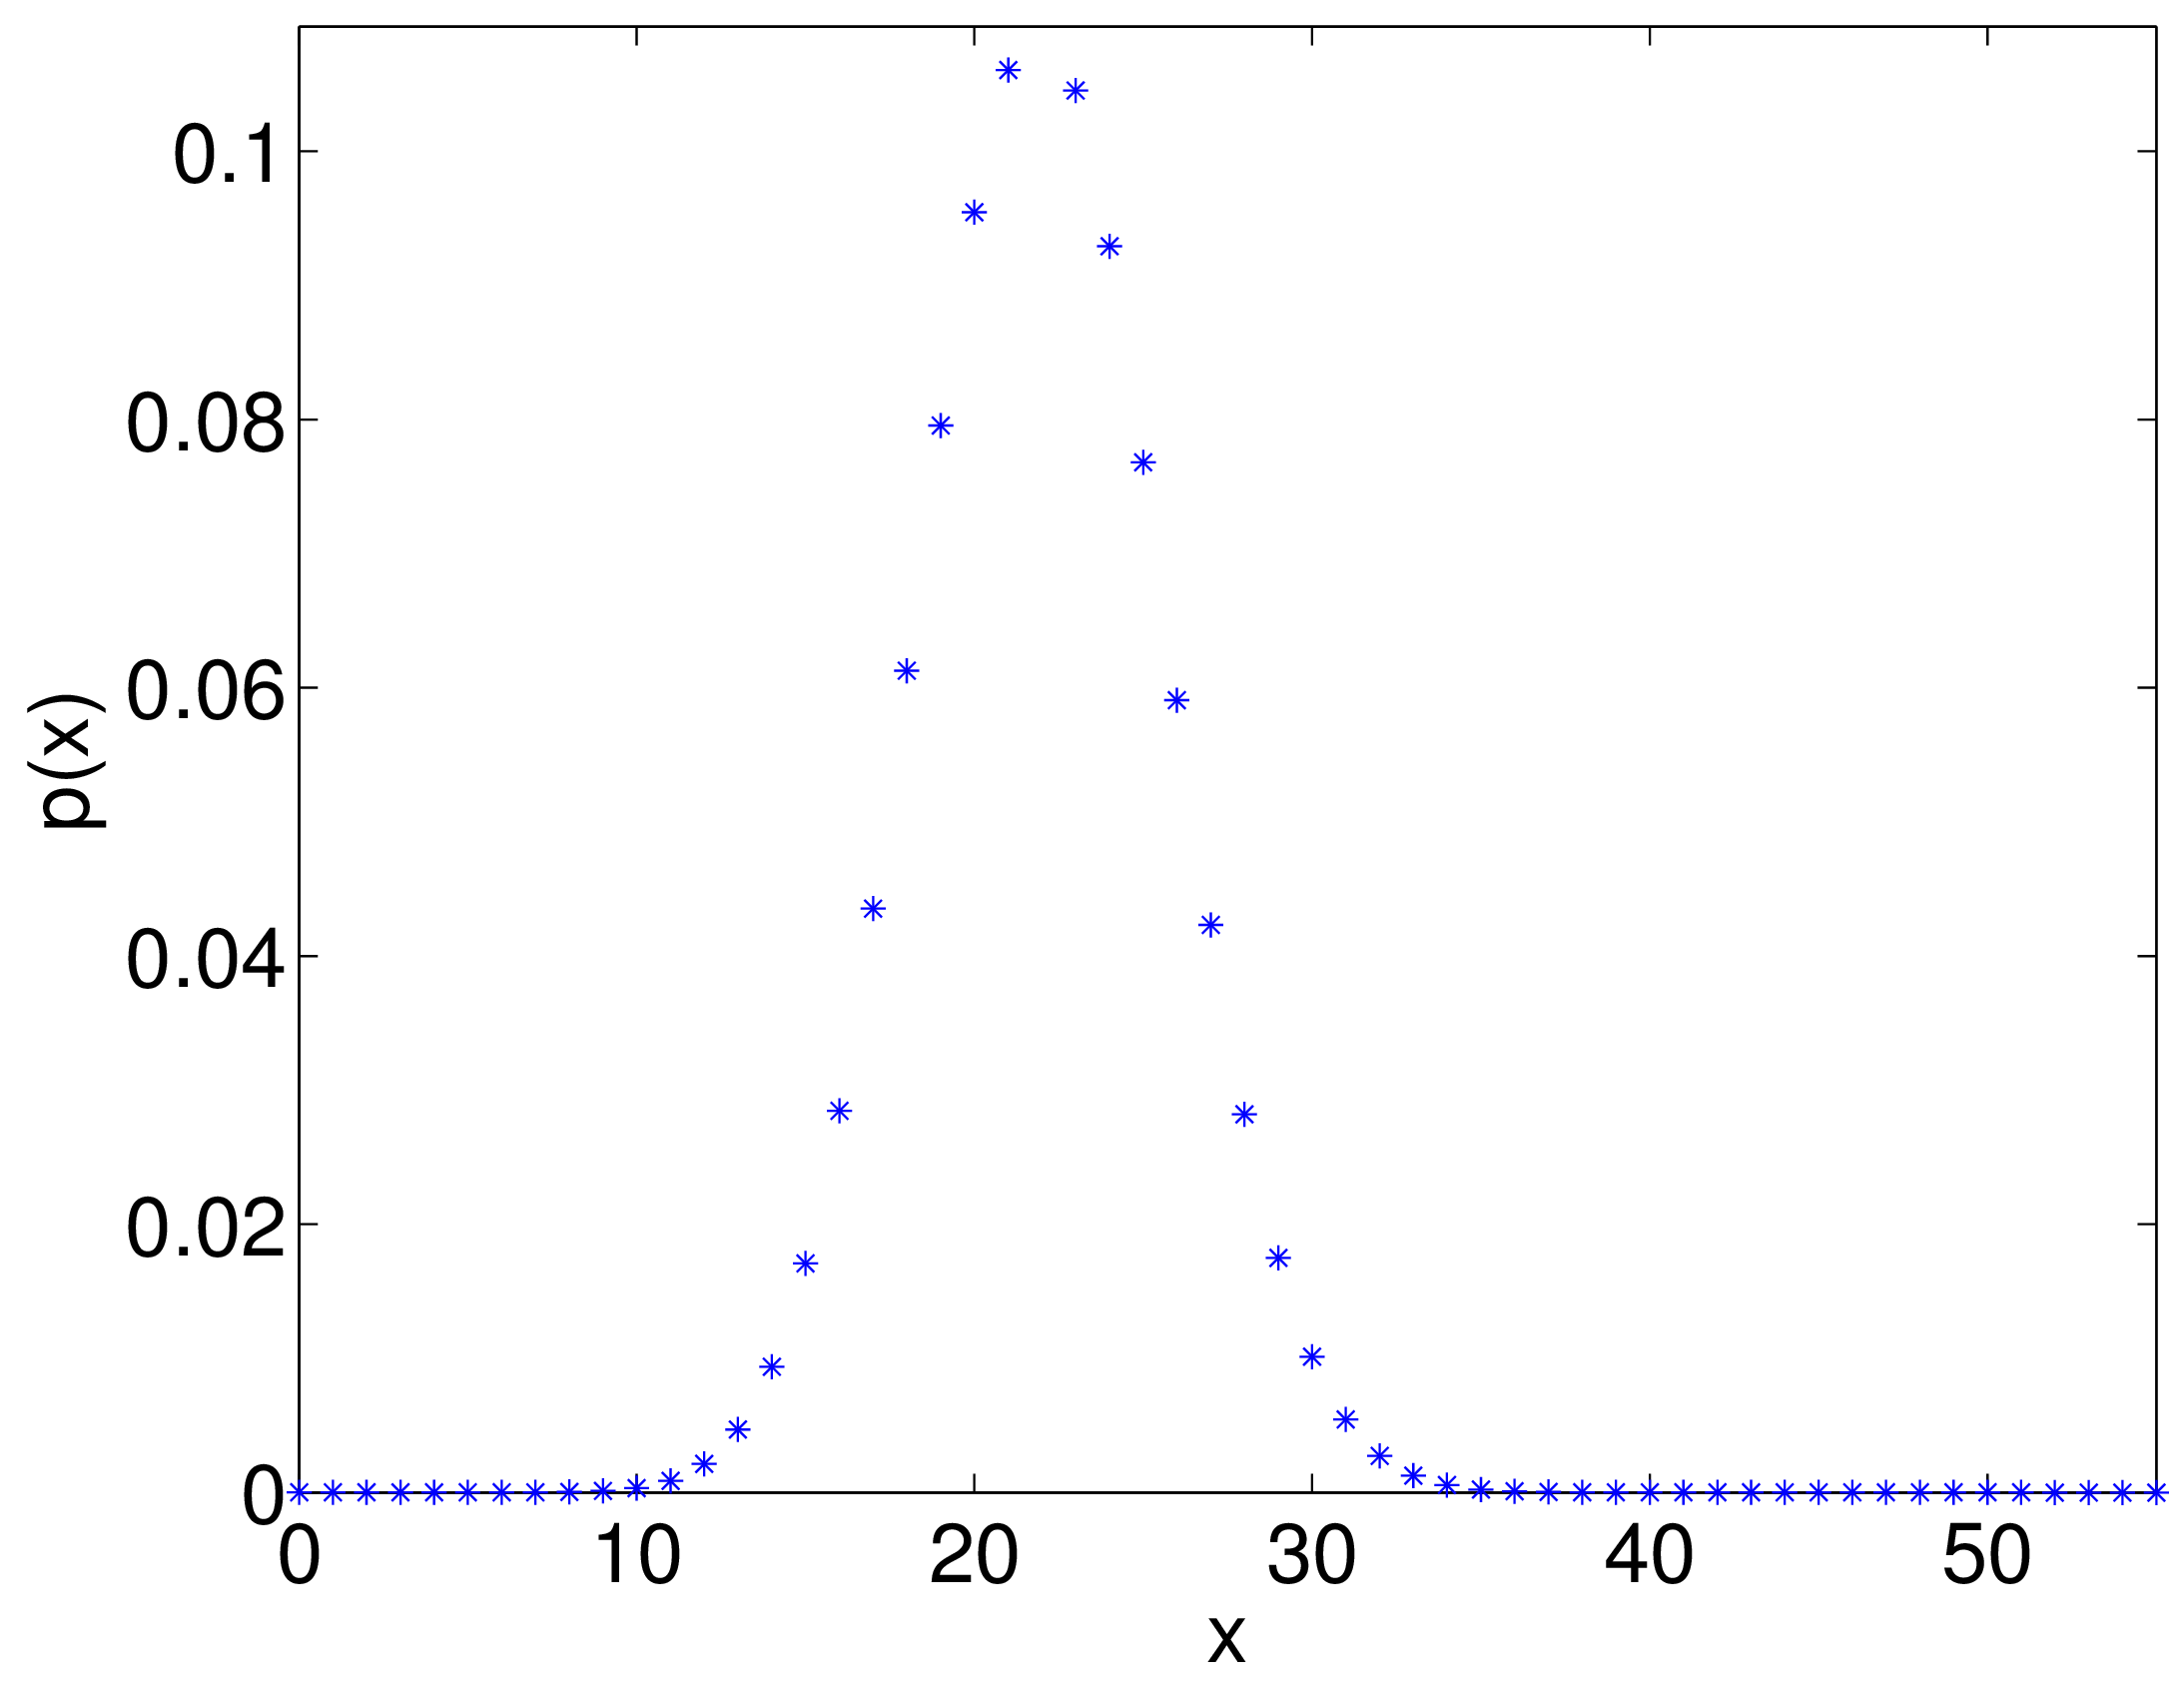
\includegraphics[scale=0.5]{vpbin11} }

\end{frame}

\begin{frame}[fragile]\frametitle{The binomial pdf}

\center{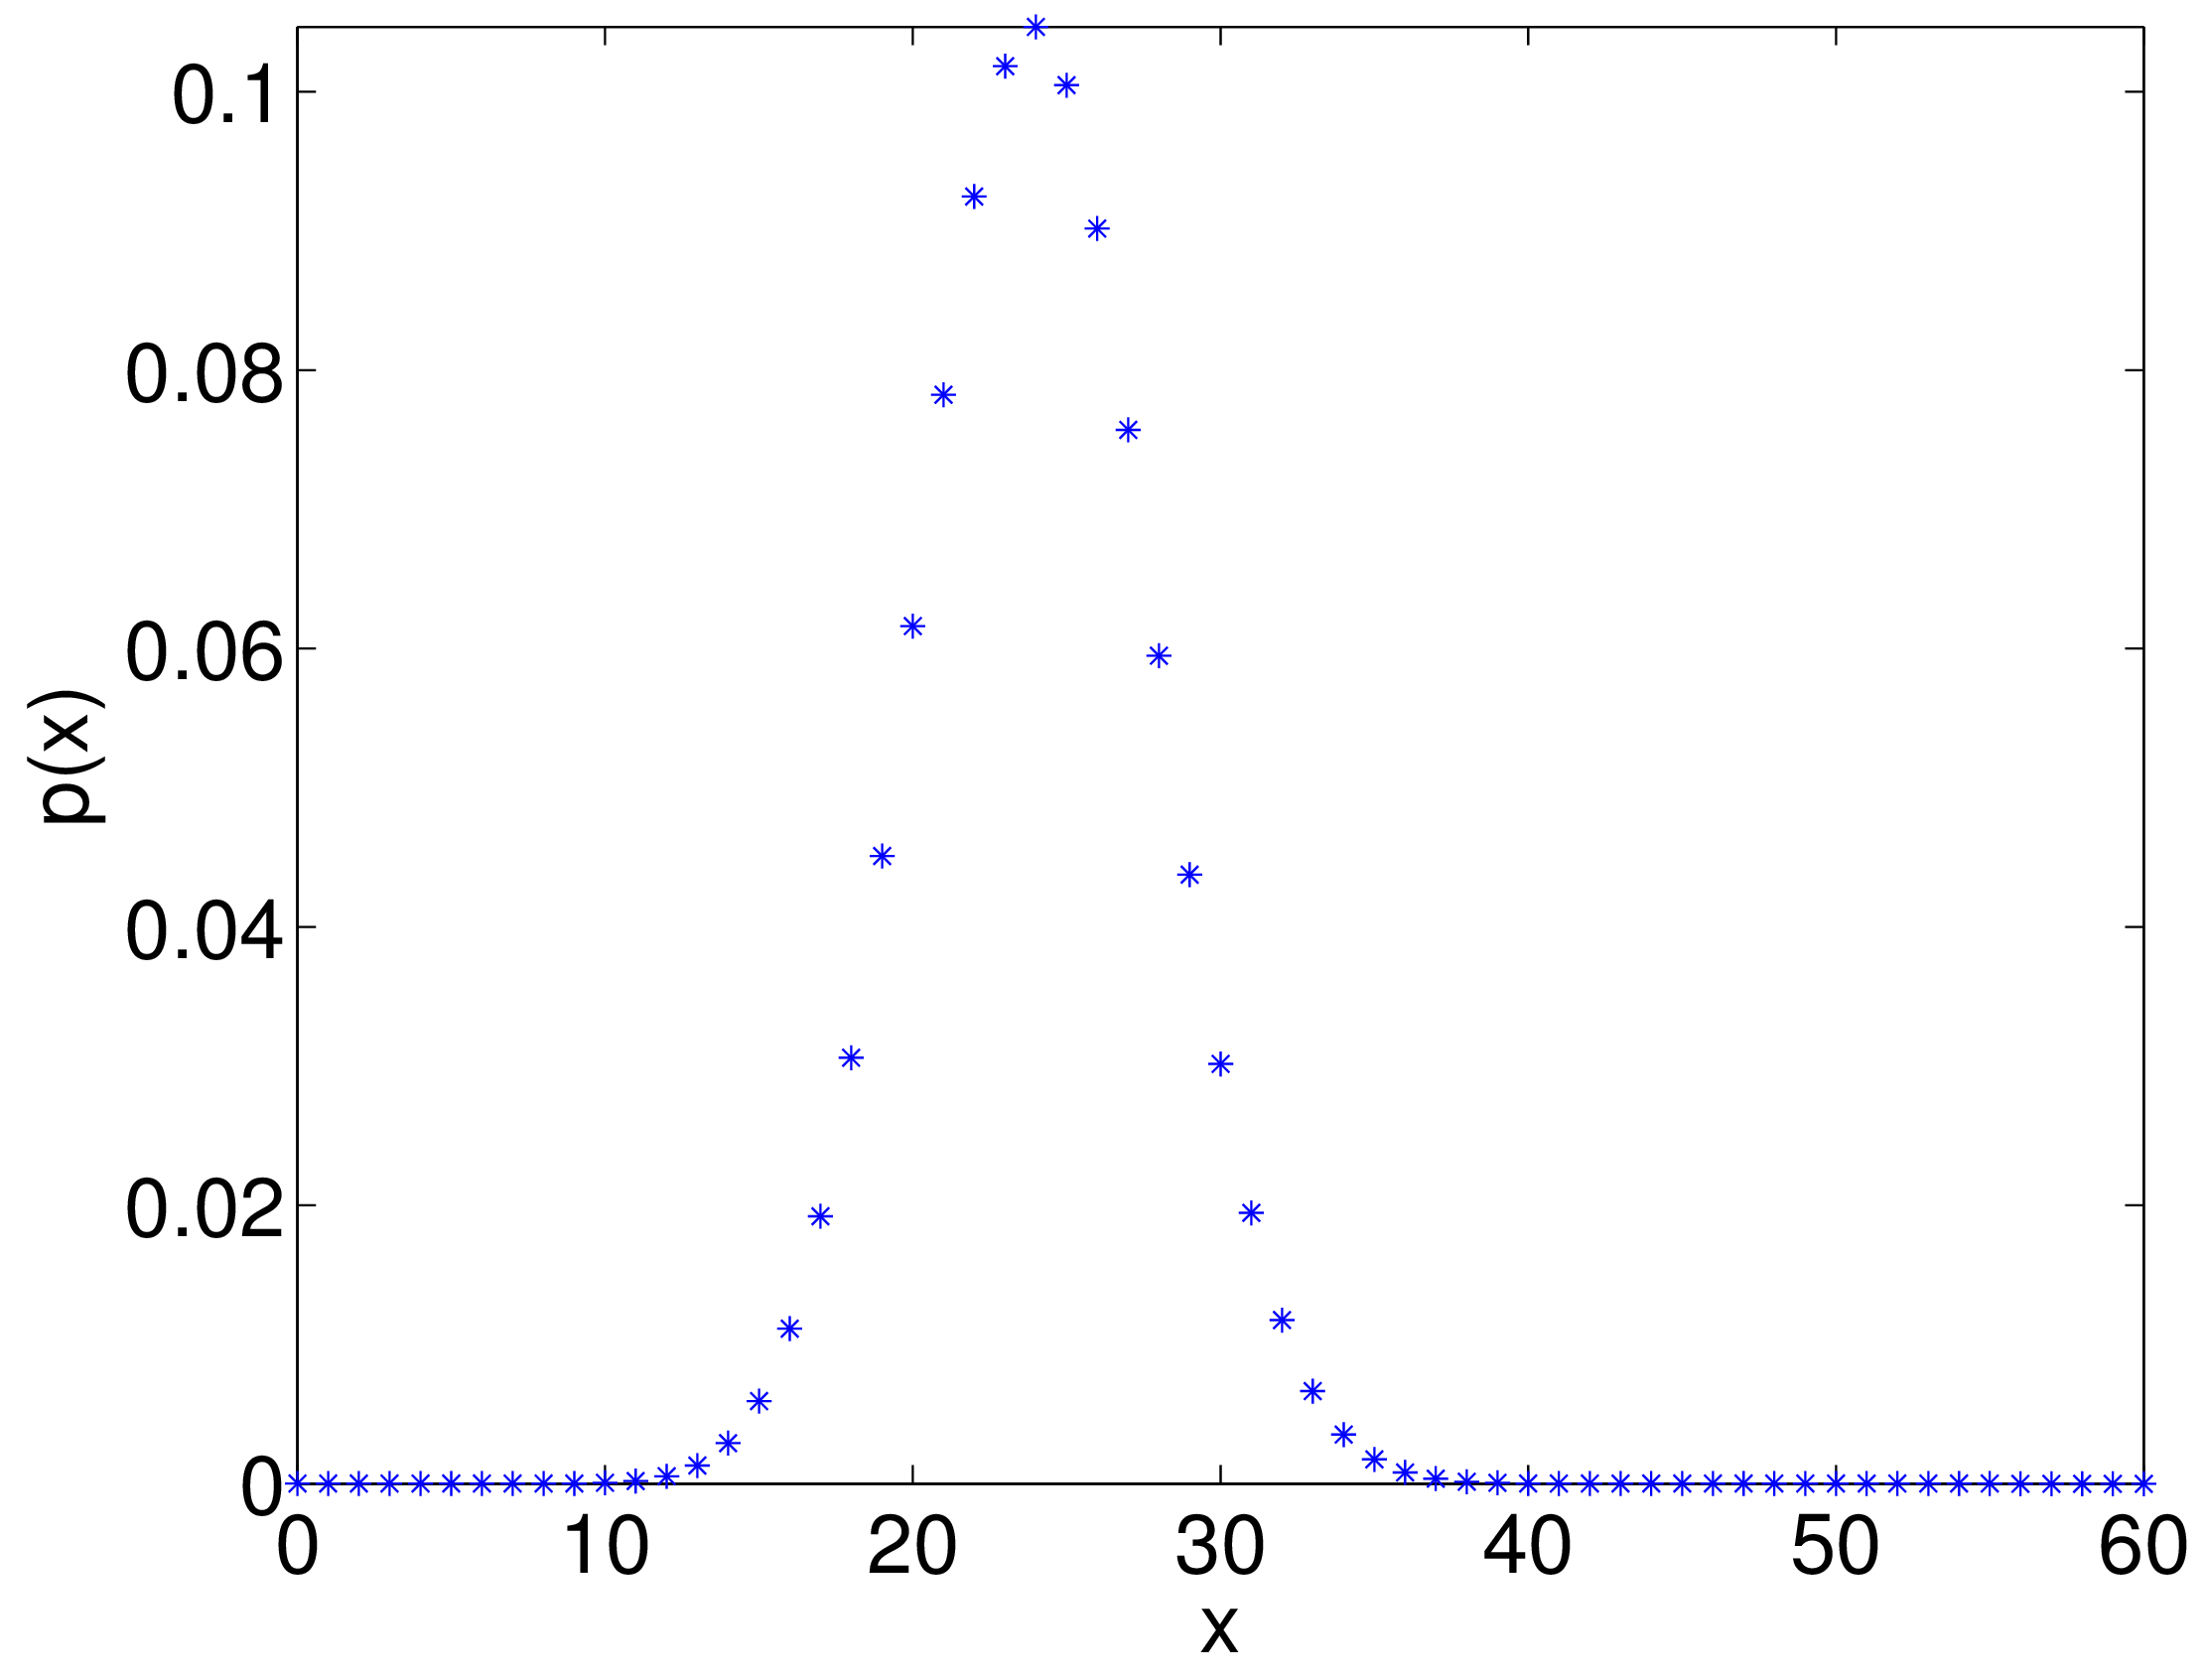
\includegraphics[scale=0.5]{vpbin12} }

\end{frame}

\begin{frame}[fragile]\frametitle{The binomial pdf}

\center{\includegraphics[scale=0.5]{vpbin13} }

\end{frame}

\begin{frame}[fragile]\frametitle{The binomial pdf}

\center{\includegraphics[scale=0.5]{vpbin14} }

\end{frame}

\begin{frame}[fragile]\frametitle{The binomial pdf}

\center{\includegraphics[scale=0.5]{vpbin15} }

\end{frame}

\begin{frame}[fragile]\frametitle{The binomial pdf}

\center{\includegraphics[scale=0.5]{vpbin16} }

\end{frame}

\begin{frame}[fragile]\frametitle{The binomial pdf}

\center{\includegraphics[scale=0.5]{vpbin17} }

\end{frame}

\begin{frame}[fragile]\frametitle{The binomial pdf}

\center{\includegraphics[scale=0.5]{vpbin18} }

\end{frame}

\begin{frame}[fragile]\frametitle{The binomial pdf}

\center{\includegraphics[scale=0.5]{vpbin19} }

\end{frame}

\begin{frame}[fragile]\frametitle{The binomial pdf}

\center{\includegraphics[scale=0.5]{vpbin20} }

\end{frame}



\begin{frame}[fragile]\frametitle{Matlab code}

{\tiny

\begin{lstlisting}
 p=.4; \\
 \textcolor{keyword}{for} i=1:20\\
   n = i*5;\\
   x= 0:n;\\
   y=binopdf(x,n,p);\\
   ym = max(y);\\
   figure(i);\\
   plot(x,y,'*');\\
   h=gca;\\
   set(h,'FontSize',[20]);\\
   set(h,'XLim',[0 n]);\\
   set(h,'YLim',[0 ym]);\\
   xlabel('x');  \\
   ylabel('p(x)'); \\
   filename = sprintf('vpbin\%d',i);\\
   saveas(h,filename,'psc2') \\
 \textcolor{keyword}{end}
\end{lstlisting}
}
\end{frame}



\begin{frame}[fragile]\frametitle{The binomial pdf}

Fix $pn= 4$ and vary $n$. 

\end{frame}



\begin{frame}[fragile]\frametitle{The binomial pdf}

\center{\includegraphics[scale=0.5]{vbbin1} }

\end{frame}

\begin{frame}[fragile]\frametitle{The binomial pdf}

\center{\includegraphics[scale=0.5]{vbbin2} }

\end{frame}

\begin{frame}[fragile]\frametitle{The binomial pdf}

\center{\includegraphics[scale=0.5]{vbbin3} }

\end{frame}

\begin{frame}[fragile]\frametitle{The binomial pdf}

\center{\includegraphics[scale=0.5]{vbbin4} }

\end{frame}

\begin{frame}[fragile]\frametitle{The binomial pdf}

\center{\includegraphics[scale=0.5]{vbbin5} }

\end{frame}

\begin{frame}[fragile]\frametitle{The binomial pdf}

\center{\includegraphics[scale=0.5]{vbbin6} }

\end{frame}

\begin{frame}[fragile]\frametitle{The binomial pdf}

\center{\includegraphics[scale=0.5]{vbbin7} }

\end{frame}

\begin{frame}[fragile]\frametitle{The binomial pdf}

\center{\includegraphics[scale=0.5]{vbbin8} }

\end{frame}

\begin{frame}[fragile]\frametitle{The binomial pdf}

\center{\includegraphics[scale=0.5]{vbbin9} }

\end{frame}

\begin{frame}[fragile]\frametitle{The binomial pdf}

\center{\includegraphics[scale=0.5]{vbbin10} }

\end{frame}

\begin{frame}[fragile]\frametitle{The binomial pdf}

\center{\includegraphics[scale=0.5]{vbbin11} }

\end{frame}

\begin{frame}[fragile]\frametitle{The binomial pdf}

\center{\includegraphics[scale=0.5]{vbbin12} }

\end{frame}

\begin{frame}[fragile]\frametitle{The binomial pdf}

\center{\includegraphics[scale=0.5]{vbbin13} }

\end{frame}

\begin{frame}[fragile]\frametitle{The binomial pdf}

\center{\includegraphics[scale=0.5]{vbbin14} }

\end{frame}

\begin{frame}[fragile]\frametitle{The binomial pdf}

\center{\includegraphics[scale=0.5]{vbbin15} }

\end{frame}

\begin{frame}[fragile]\frametitle{The binomial pdf}

\center{\includegraphics[scale=0.5]{vbbin16} }

\end{frame}

\begin{frame}[fragile]\frametitle{The binomial pdf}

\center{\includegraphics[scale=0.5]{vbbin17} }

\end{frame}

\begin{frame}[fragile]\frametitle{The binomial pdf}

\center{\includegraphics[scale=0.5]{vbbin18} }

\end{frame}

\begin{frame}[fragile]\frametitle{The binomial pdf}

\center{\includegraphics[scale=0.5]{vbbin19} }

\end{frame}

\begin{frame}[fragile]\frametitle{The binomial pdf}

\center{\includegraphics[scale=0.5]{vbbin20} }

\end{frame}


\begin{frame}[fragile]\frametitle{Matlab code}

{\tiny

\begin{lstlisting}
 val=4; \\
 \textcolor{keyword}{for} i=1:20\\
   n = i*5;\\
   p = val/n; \\
   x= 0:n;\\
   y=binopdf(x,n,p);\\
   ym = max(y);\\
   figure(i);\\
   plot(x,y,'*');\\
   h=gca;\\
   set(h,'FontSize',[20]);\\
   set(h,'XLim',[0 n]);\\
   set(h,'YLim',[0 ym]);\\
   xlabel('x');  \\
   ylabel('p(x)'); \\
   filename = sprintf('vbbin\%d',i);\\
   saveas(h,filename,'psc2') \\
 \textcolor{keyword}{end}
\end{lstlisting}
}
\end{frame}




\begin{frame}[fragile]\frametitle{Binomial cdf}

\begin{thm}
If $X \sim \mbox{Bin}(n,p)$ the cdf is denoted
$$\pr(X \leq x) = \mbox{Bin}(x;n,p) = \sum_{i=0}^x \binom{n}{i} p^i (1-p)^{n-i} \, \, \, \, \, x=0,1,...,n.$$ 
\end{thm}


\end{frame}



\begin{frame}[fragile]\frametitle{Binomial cdf}

Example:

I give you an exam and there are $n=120$ of you. The probability
someone fails is $p=.1$. \\ 

What is the probability that at most $12$ fail the test ?  
$$\mbox{Bin}(12;120,.1) =  \sum_{i=0}^{12} \binom{120}{i}\times (.1)^i
\times (.9)^{120-i}.$$


\end{frame}



\begin{frame}[fragile]\frametitle{Binomial pdf}

If $X \sim \mbox{Bin}(n,p)$ what is $\mathbb E[X]$ ?  
$$\mathbb E[X] = \mathbb E[X_1]+\mathbb E[X_2]+\mathbb E[X_3]+ ... + \mathbb E[X_n],$$
where $X_i$ is a Bernoulli random variable. \\ 
$$\mathbb E[X_i] = p,$$
so
$$\mathbb E[X] = np.$$ 

\end{frame}



\begin{frame}[fragile]\frametitle{Binomial pdf}

If $X \sim \mbox{Bin}(n,p)$ what is $\mathbb V[X]$ ?  
\begin{eqnarray*}
\mathbb V[X]& =& \mathbb V[X_1+X_2+X_3+ ... +X_n],\\
      &= &\mathbb V[X_1]+\mathbb V[X_2]+\mathbb V[X_3]+ ... + \mathbb V[X_n],
\end{eqnarray*}
where $X_i$ is an independent Bernoulli random variable. \\ 
$$\mathbb V[X_i] = p(1-p),$$
so
$$\mathbb V[X] = np(1-p).$$ \\ 

\end{frame}


%%%%%%%%%%%%%%%%%%%%%%%%%%%%%%%%%%%%%%%%%%%%%%%%%%%%%%%%%%%%%%%%%%%%%%%%%%%%%%%%%%
\begin{frame}[fragile]\frametitle{}
\begin{center}
{\Large Hypergeometric}

\end{center}
\end{frame}



\begin{frame}[fragile]\frametitle{Sampling without replacement}

This time the urn full of m\&ms are put in a room with some extremely intelligent and highly civilized people.

\center{\includegraphics[scale=0.25]{bb} }

\end{frame}


\begin{frame}[fragile]\frametitle{Sampling without replacement}

There are $N=500$ m\&ms in the urn and $M=200$ are red. \\ 
Each day for $n=40$ days, whenever they find some time from drama, they remove one m\&m from
the urn (having fought over it). \\ 
Since we don't trust them, we interfere and record the color of the m\&m picked and then leave them alone. \\ 
Of course they cannot resist the temptation and eat that picked m\&m (having again fought over it).

\end{frame}


\begin{frame}[fragile]\frametitle{Sampling without replacement}

This procedure is sampling without replacement and the distribution of the
number of red m\&ms drawn after $40$ days is a hypergeometric
distribution parameterized as $\mbox{hyp}(x;N,M,n).$

\end{frame}




\begin{frame}[fragile]\frametitle{Sampling without replacement}

\begin{enumerate}

\item The population to be sampled consists of $N$ objects. 

\item Each object is either a $0$ or a $1$ and there are
$M$ $1$'s. Each trial is Bernoulli. The probability of selecting
a $1$ is $p=\frac{M}{N}$. 

\item A sample of $n$ objects is selected without replacement such
  that each subset of size $n$ of the $N$ objects is equally likely. 

\end{enumerate}

The rv $X$ is the number of $1$'s in the $n$ objects drawn and
$X \sim \mbox{Hyp}(n,M,N)$. \\ 

What is the probability density function $p(x)$ ?

\end{frame}



\begin{frame}[fragile]\frametitle{Pdf of the hypergeometric}

\begin{eqnarray*}
\pr(X=x) & =&  \mbox{hyp}(x;n,M,N) \\ 
 & =&  \frac{\mbox{number of outcomes with $x$ $1$'s}}{\mbox{total
     number of outcomes}} \\ 
& =&  \frac{\binom{M}{x} \binom{N-M}{n-x}}{\binom{N}{n}}. 
\end{eqnarray*}

The denominator is the total number of outcomes or ways to choose
$n$ out of $N$ objects without considering order. \\ 

The numerator has two terms:\\
$\binom{M}{x}$ is the number of ways of selecting $x$ $1$'s out of
$M$ $1$'s without considering order. \\ 
$\binom{N-M}{n-x}$ is the number of ways of selecting $n-x$ $0$'s
out of $N-M$ $0$'s  without considering order.

\end{frame}


\begin{frame}[fragile]\frametitle{Pdf of the hypergeometric}

\begin{prop}
If $X$ is the number of $1$'s in a random sample of size $n$ drawn
from a population of $M$ $1$'s and $N-M$ $0$'s then the probability
distribution of $X$ called the {\bf hypergeometric distribution}
is
$$\mbox{hyp}(x;n,M,N) = \frac{\binom{M}{x}
  \binom{N-M}{n-x}}{\binom{N}{n}},$$
where $\max(0,n-N+M) \leq x \leq \min(n,M)$.

\end{prop}

\end{frame}


\begin{frame}[fragile]\frametitle{Example: a genetic screen}

A genetic screen of $1000$ genes is run to check for association
with diabetes and it is found that $40$ genes of the $1000$ are
associated with the occurance of diabetes. \\ 

Genes in the oxidative phosphorylation (OXPHOS) pathway are
thought to be implicated in diabetes due to their effect on
metabolism. There are $60$ genes in this pathway all of which
were included in the initial screen. \\ 


The overlap between genes in the OXPHOS pathway and the genes
that associate with diabetes is $35$. Does this imply that
genes in the OXPHOS pathway are enriched or associated with
diabetes ? 

\end{frame}


\begin{frame}[fragile]\frametitle{Example: a genetic screen}

$N=1000$ objects\\ 
$x=35$ genes associated with diabetes and OXPHOS \\ 
$n=40$ genes randomly sampled (found to be associated with diabetes)
\\ 
$M=60$ genes associated with OXPHOS \\ 

Out of $1000$ objects of which $60$ belong to OXPHOS if I randomly
sample $40$ will $35$ of them be OXPHOS ? \\ 


$$\mbox{hyp}(35;40,60,1000) = 5.6503 \cdot 10^{-43}.$$
So very unlikely by chance so OXPHOS and diabetes might
be associated.

\end{frame}



\begin{frame}[fragile]\frametitle{Hypergeometric pdf}

If $X \sim \mbox{Hyp}(n,M,N)$ what is $\mathbb E[X]$ ?  
$$\mathbb E[X] = \mathbb E[X_1]+\mathbb E[X_2]+\mathbb E[X_3]+ ... + \mathbb E[X_n],$$
where $X_i$ is a Bernoulli random variable. \\ 
$$\mathbb E[X_i] = p = \frac{M}{N},$$
so
$$\mathbb E[X] = n \cdot \frac{M}{N}.$$ 

\end{frame}



\begin{frame}[fragile]\frametitle{Hypergeometric pdf}

If $X \sim \mbox{Hyp}(n,M,N)$ what is $\mathbb V[X]$ ?  
\begin{eqnarray*}
\mathbb V[X]& =& \mathbb V[X_1+X_2+X_3+ ... +X_n],\\
      & < &\mathbb V[X_1]+\mathbb V[X_2]+\mathbb V[X_3]+ ... + \mathbb V[X_n],
\end{eqnarray*}
because $X_i$ are not independent Bernoulli random variables. \\ 
$$\mathbb V[X] = \frac{N-n}{N-1} \cdot np(1-p) ,$$ 
where $\frac{N-n}{N-1} < 1$ is the correction factor and approaches 
$1$ when $N \gg n$.

\end{frame}


%%%%%%%%%%%%%%%%%%%%%%%%%%%%%%%%%%%%%%%%%%%%%%%%%%%%%%%%%%%%%%%%%%%%%%%%%%%%%%%%%%
\begin{frame}[fragile]\frametitle{}
\begin{center}
{\Large Poisson}

\end{center}
\end{frame}



\begin{frame}[fragile]\frametitle{Sim\'eon Poisson}

\center{\includegraphics[scale=0.2]{Simeon_Poisson} }

\end{frame}



\begin{frame}[fragile]\frametitle{Poisson distribution}

\begin{defn}

A random variable $X$ is said to have a  {\bf Poisson distribution}
with parameter $\lambda >0$ if the pdf of $X$ is
$$\mbox{Pois}(x;\lambda) = \frac{e^{-\lambda} \lambda^x}{x!}, \, \, \,
\, \, \, \, x=0,1,2,3,...$$ 
\end{defn}


\end{frame}


\begin{frame}[fragile]\frametitle{Properties of the Poisson pdf}

$$\sum_{x=0}^\infty \frac{e^{-\lambda} \lambda^x}{x!} = 1$$
By a series expansion
$$e^{\lambda} = 1 + \lambda + \frac{\lambda^2}{2!} +
\frac{\lambda^3}{3!} +... = \sum_{x=0}^\infty \frac{\lambda^x}{x!}.$$
Therefore 
$$e^{-\lambda} \sum_{x=0}^\infty \frac{\lambda^x}{x!} = 1.$$

\end{frame}



\begin{frame}[fragile]\frametitle{Properties of the Poisson pdf}

The mean and variance of the Poisson distribution is
$$\mathbb E[X] = \mathbb V[X] = \lambda.$$

\end{frame}


\begin{frame}[fragile]\frametitle{Parameter $\lambda$}


$\lambda$ is a positive real number, equal to the expected number 
of occurrences that occur during the given interval. \\ 

For instance, if the events occur on average every $4$ minutes, and 
you are interested in the number of events occurring in a $10$ 
minute interval, you would use as model a Poisson distribution with 
$\lambda = 10/4 = 2.5$.

\end{frame}


\begin{frame}[fragile]\frametitle{Things modeled using Poisson distribution}

Examples

\begin{enumerate}
\item The number of soldiers killed by horse-kicks each year in each 
corps in the Prussian cavalry. 

\item The number of spelling mistakes one makes while typing a single
  page. 

\item The number of phone calls at a call center per minute. 

\item The number of times a web server is accessed per minute. 

\item The number of roadkill (animals killed) found per unit length of
  road. 

\item The number of mutations in a given stretch of DNA after a
  certain amount of radiation.
 
\end{enumerate}
\end{frame}



\begin{frame}[fragile]\frametitle{Poisson distribution as binomial limit}


\begin{thm}

If we take the binomial pdf $\mbox{bin}(x;n,p)$ and
take the limit $\lim_{n \rightarrow \infty, p \rightarrow 0} np =
\lambda >0$ then 
$$\mbox{bin}(x;n,p) \rightarrow \mbox{Pois}(x;\lambda).$$
\end{thm}

\end{frame}


\begin{frame}[fragile]\frametitle{Some pictures}
\center{\includegraphics[scale=0.5]{binapprox1} }
\end{frame}

\begin{frame}[fragile]\frametitle{Some pictures}
\center{\includegraphics[scale=0.5]{binapprox2} }
\end{frame}

\begin{frame}[fragile]\frametitle{Some pictures}
\center{\includegraphics[scale=0.5]{binapprox3} }
\end{frame}

\begin{frame}[fragile]\frametitle{Some pictures}
\center{\includegraphics[scale=0.5]{binapprox4} }
\end{frame}

\begin{frame}[fragile]\frametitle{Some pictures}
\center{\includegraphics[scale=0.5]{binapprox5} }
\end{frame}

\begin{frame}[fragile]\frametitle{Some pictures}
\center{\includegraphics[scale=0.5]{binapprox6} }
\end{frame}




\begin{frame}[fragile]\frametitle{Matlab code}

{\tiny

\begin{lstlisting}
 \textcolor{keyword}{for} i=1:6 \\
 
 figure(i)\\
 n=300;\\
 x= 0:n;\\
 lambda = i*10;\\
 y=poisspdf(x,lambda);\\
 y1 = max(y);\\
 plot(x,y,'*'); \\
 hold on\\
 y=binopdf(x,n,lambda/n);\\
 y2 = max(y);\\
 ym=max(y1,y2);\\
 plot(x,y,'r*');\\
 h=gca;\\
 set(h,'FontSize',[20]);\\
 xlabel('x');\\
 ylabel('p(x)');\\
 set(h,'XLim',[0 n]);\\
 set(h,'YLim',[0 ym]);\\
 hold off\\
 filename = sprintf('binapprox\%d',i);\\
 saveas(h,filename,'psc2');\\

 \textcolor{keyword}{end}
\end{lstlisting}
}
\end{frame}


\begin{frame}[fragile]\frametitle{Poisson process}

The Poisson process is defined in terms of occurence of events and
is a function of the counts of events as a function of time,
$N(t)$. \\ 

The basic idea is that there is a rate parameter $\lambda$ and 
the number of events in the time $(t,t+\tau]$ follows a Poisson
distribution with parameter $\lambda \tau$ 
$$\pr[(N(t+\tau)-N(t)) = k] = \frac{e^{-\lambda \tau} (\lambda
  \tau)^k}{k!} \, \, \, \, \, \, \, \, k=0,1,2,...,$$
where $N(t+\tau)-N(t)$ describes the number of events in 
the time interval $(t,t+\tau]$. \\ 

The above is a Poisson process, not a density or distribution 
function.

\end{frame}



\begin{frame}[fragile]\frametitle{Poisson process}

The general properties of a (homogenous) Poisson process are

\begin{enumerate}

\item Memorylessness:  The number of arrivals occurring during the time
  interval $t+\tau$ is independent of the number of arrivals occurring 
  before time $t$; 

\item Orderliness: Arrivals do not occur simultaneously
$$\lim_{\tau \rightarrow 0} P[N(t+\tau) - N(t) > 1 | N(t+\tau) -N(t)
\geq 1] = 0;$$  

\item Homogeniety: The probability that exactly one event happens
in the time interval $\tau$ is $\lambda \tau$  
$$\pr[N(t+\tau)-N(t) = 1] = \lambda \tau +o(\tau).$$ 

\end{enumerate}

\end{frame}




\begin{frame}[fragile]\frametitle{Example}

Telephone call arrivals:\\
Call requests arrive at times $T_1,T_2,...$ \\
What we have access to is $N(t)$ or the number of
that arrive in time $t$. \\ 
Suppose that the counts are distributed as a Poisson
process with rate parameter $\lambda=4$ per min. \\  

\begin{enumerate}
\item What is the probability of exactly $140$ arrivals
in $30$ minutes ? 

\item What is the expected value of the number of calls
in a $30$ minute interval ? 

\end{enumerate}

\end{frame}




\begin{frame}[fragile]\frametitle{Example}

What is the probability of exactly $10$ arrivals
in $30$ minutes ? \\ 

\begin{eqnarray*}
\pr[(N(t+\tau)-N(t)) = k] &=& \frac{e^{-\lambda \tau} (\lambda \tau)^k}{k!} \, \, \, \, \, \, \, \, k=0,1,2,..., \\
\pr[N(30) = 140] & = & \frac{e^{-4 \cdot 30}(4 \cdot  30)^{140}}{140!}.\\
& = & 0.0069.
\end{eqnarray*}

\end{frame}



\begin{frame}[fragile]\frametitle{Example}

What is the expected value of the number of calls
in a $30$ minute interval ? \\ 

\begin{eqnarray*}
\mathbb E[N(30)] &= &\sum_{k=0}^{\infty} k \, \pr[N(30) = k] \\ 
 &=& \sum_{k=0}^\infty k \, \frac{e^{-120} 120^k}{k!}. \\ 
& = & 120. 
\end{eqnarray*}

\begin{lstlisting} 
 val = 0;\\
  for k=0:10000 \\
   val = val + k*poisspdf(k,120);\\
end
\end{lstlisting}

\end{frame}

%%%%%%%%%%%%%%%%%%%%%%%%%%%%%%%%%%%%%%%%%%%%%%%%%%%%%%%%%%%%%%%%%%%%%%%%%%%%%%%%%%
\begin{frame}[fragile]\frametitle{}
\begin{center}
{\Large Continuous random variables}

\end{center}
\end{frame}



\begin{frame}[fragile]\frametitle{Mathematical definition}

\begin{defn}
A random variable $X$ is continuous if its set of possible values is an
entire interval of real numbers: $x \in [A,B]$ for $A < B$. 
\end{defn}

\end{frame}


\begin{frame}[fragile]\frametitle{Examples}

\begin{enumerate}

\item Heights of people. 

\item Amount of rainfall per square meter. 

\item IQ scores. 

\end{enumerate}


\end{frame}

\begin{frame}[fragile]\frametitle{Probability distributions}

\begin{defn}
Let $X$ be a continuous rv. The {\bf probability density function}
(pdf) of $X$ is a function $p(x)$ such that for any two numbers
$a \leq b$
$$\pr(a \leq X \leq b) = \int_a^b p(x) \, dx.$$ 

The probability that $X$ takes values in the interval $[a,b]$ 
is the area under the graph of the density function in the
interval.  
\end{defn}



\end{frame}

\begin{frame}[fragile]\frametitle{Picture}

\center{\includegraphics[scale=0.7]{Normal3} }

\end{frame}



\begin{frame}[fragile]\frametitle{Restatement}

\begin{prop}
Let $X$ be a continuous rv. Then for any number $c$, $\pr(X=c) = 0$
and for any two numbers $a<b$
\begin{eqnarray*}
\pr(a \leq X \leq b) & = &\pr(a < X \leq b)  \\
 & = &\pr(a \leq X < b)  \\
& = &\pr(a < X < b).
\end{eqnarray*}
\end{prop}



\end{frame}


\begin{frame}[fragile]\frametitle{Cumulative distribution function}
\begin{defn}
The {\bf cumulative distribution function} (cdf) $F(x)$ for
a continuous rv $X$ is defined for every number $x$ by
$$F(x) = \pr(X \leq x) = \int_{-\infty}^x p(u) du.$$ 

So for for each $x$, $F(x)$ is the area under the density
to the left of $x$.
\end{defn}



\end{frame}



\begin{frame}[fragile]\frametitle{Picture}

\center{\includegraphics[scale=0.4]{cdfpdf} }


\end{frame}


\begin{frame}[fragile]\frametitle{Matlab code}

\begin{tabbing}
x= -10:.01:10; \\
y = normpdf(x,.5,1);\\
plot(x,y,'r');\\
hold on;\\
y1 = normcdf(x,.5,1);\\
plot(x,y1,'b');\\
\end{tabbing}
\end{frame}





\begin{frame}[fragile]\frametitle{More properties}

\begin{prop}
Let $X$ be a continuous rv with pdf $p(x)$ and cdf $F(x)$. Then for
any number $a$,
$$\pr(X > a) = 1- F(a),$$ 
and for any two numbers $a<b$,
$$\pr(a \leq X \leq b) = F(b)-F(a).$$
\end{prop} 


\end{frame}

\begin{frame}[fragile]\frametitle{More properties}

\begin{thm}[Radon-Nikodym]
Let $X$ be a continuous rv with pdf $p(x)$ and cdf $F(x)$. Then at
every $x$ at which $F'(x)$ exists, $F'(x) = p(x)$.
\end{thm} 



\end{frame}


\begin{frame}[fragile]\frametitle{Picture}

\center{\includegraphics[scale=0.4]{cdfpdf1} }


\end{frame}

\begin{frame}[fragile]\frametitle{Erf}

\center{\includegraphics[scale=0.4]{cdfpdf} }


\end{frame}


\begin{frame}[fragile]\frametitle{Matlab code}

\begin{tabbing}
x= 0:.01:.2; \\
y = unipdf(x,0,2);\\
plot(x,y,'r');\\
hold on;\\
y1 = unicdf(x,0,2);\\
plot(x,y1,'b');\\
\end{tabbing}
\end{frame}


\begin{frame}[fragile]\frametitle{Matlab code}

\begin{tabbing}
x= -10:.01:10; \\
y = normpdf(x,.5,1);\\
plot(x,y,'r');\\
hold on;\\
y1 = normcdf(x,.5,1);\\
plot(x,y1,'b');\\
\end{tabbing}
\end{frame}



\begin{frame}[fragile]\frametitle{Reprise}


The opposite of integrate is differentiate. 

\begin{prop}
\begin{eqnarray*}
F(x) &=& \int_{-\infty}^x p(u) du,  \\
F'(x)& =& p(x).
\end{eqnarray*}

\end{prop}
\end{frame}


\begin{frame}[fragile]\frametitle{Mean}

\begin{defn}
The {\bf expected} or {\bf mean value} of a continuous rv $X$ with
pdf $p(x)$ is
$$\mu_{_X} = \bE(X) = \int_{-\infty}^{\infty} x \, p(x) dx,$$
and the expectation of a function $h(x)$ is
$$\mu_{_{h(X)}} = \mathbb E[h(x)] = \int_{-\infty}^{\infty} h(x) \, p(x) dx.$$

\end{defn}

\end{frame}



\begin{frame}[fragile]\frametitle{Variance}

\begin{defn}
The {\bf variance} of a continuous rv $X$ with
pdf $p(x)$ is
$$\sigma^2_{_X} = \mathbb V(X) = \int_{-\infty}^{\infty} (x - \mu)^2\, p(x) dx,$$
and the {\bf standard deviation} is $\sigma_{_X}$. 
\end{defn}

\end{frame}


\begin{frame}[fragile]\frametitle{Percentiles}

\begin{defn}
Let $p$ be a number between $0$ and $100$ the {\bf $p$-th percentile}
of the distribution of a continuous rv $X$ is the value $a$
such that 
$$p = 100*F(a) = 100*\int_{-\infty}^{a} p(u) \, du.$$

The {\bf median} is the value $a$ for which $p=50$.
\end{defn}

\end{frame}


%%%%%%%%%%%%%%%%%%%%%%%%%%%%%%%%%%%%%%%%%%%%%%%%%%%%%%%%%%%%%%%%%%%%%%%%%%%%%%%%%%
\begin{frame}[fragile]\frametitle{}
\begin{center}
{\Large Continuous distributions: Uniform }

\end{center}
\end{frame}



\begin{frame}[fragile]\frametitle{Uniform}

For real numbers $a < b$
$$p(x;a,b) = \left\{\begin{array}{ll}
			0 & \mbox{if } x  < a \\
			\frac{1}{b-a} & \mbox{if } a \leq x < b \\
			0 & \mbox{if } x > b 
				   .	\end{array} \right
						. $$ 
\vspace{.1in}

$$F(x;a,b) = \left\{\begin{array}{ll}
			0 & \mbox{if } x  < a \\
			\frac{x-a}{b-a} & \mbox{if } a \leq x < b \\
			1 & \mbox{if } x > b 
				   .	\end{array} \right
						. $$ 



\end{frame}



\begin{frame}[fragile]\frametitle{Picture}

\center{\includegraphics[scale=0.4]{cdfpdf1} }

\end{frame}


\begin{frame}[fragile]\frametitle{Mean}

\begin{eqnarray*}
\mu_{_X} & = & \int_a^b  \frac{1}{b-a} \, x \, dx \\ 
        & = & \frac{1}{b-a} \int_a^b x \, dx \\ 
        & = & \frac{1}{b-a} \, x^2|_a^b \\ 
        & = & \frac{1}{b-a} \frac{b^2-a^2}{2} \\ 
        & = & \frac{1}{b-a} \frac{(b-a)(b+a)}{2} \\
        & = & \frac{b+a}{2}
\end{eqnarray*}

\end{frame}

\begin{frame}[fragile]\frametitle{Variance}

{\tiny
$$\sigma^2_{_X}  =  \int_a^b  \frac{1}{b-a} (x-\frac{a+b}{2})^2 \,
dx.$$ 
Change of variables $u = x-\frac{a+b}{2}$ 
\begin{eqnarray*}
\sigma^2_{_X} & = & \frac{1}{b-a} \int_{(a-b)/2}^{(b-a)/2}  u^2 \,  du
\\ 
        & = & \frac{1}{3(b-a)} \left[ \frac{(b-a)^3}{8} -
          \frac{(a-b)^3}{8}   \right] \\ 
        & = & \frac{1}{3}  \left[ \frac{(b-a)^2}{8} -
          \frac{(a-b)(b-a)}{8}   \right] \\ 
        & = & \frac{1}{3}  \left[ \frac{a^2+b^2- 2ab }{8} -
          \frac{-b^2-a^2+2ab}{8}   \right] \\ 
        & = & \frac{1}{3}  \left[ \frac{2(a-b)^2}{8} \right] \\ 
        & = & \frac{(a-b)^2}{12}
\end{eqnarray*}

}
\end{frame}


%%%%%%%%%%%%%%%%%%%%%%%%%%%%%%%%%%%%%%%%%%%%%%%%%%%%%%%%%%%%%%%%%%%%%%%%%%%%%%%%%%
\begin{frame}[fragile]\frametitle{}
\begin{center}
{\Large Continuous distributions: Normal }

\end{center}
\end{frame}



\begin{frame}[fragile]\frametitle{Normal pdf}


\begin{defn}
A continuous rv $X$ has a {\bf Gaussian} or {\bf normal distribution}
with paramaters
$-\infty < \mu < \infty$ and $0  < \sigma$ with pdf
$$p(x) = \mbox{No}(x;\mu,\sigma) = \frac{1}{\sigma \sqrt{2 \pi}} \, e^{-(x-\mu)^2/(2 \sigma^2)}
.$$
\end{defn}

\end{frame}



\begin{frame}[fragile]\frametitle{Normal cdf}

\begin{thm}
If $X \sim \mbox{N}(\mu,\sigma)$ the cdf is 
$$\pr(X \leq x) = \frac{1}{\sigma \sqrt{2 \pi}}\int_{-\infty}^x 
e^{-(z-\mu)^2/(2 \sigma^2)} dz.$$ 
\end{thm}


\end{frame}


\begin{frame}[fragile]\frametitle{Picture}

\center{\includegraphics[scale=0.4]{cdfpdf} }

\end{frame}









\begin{frame}[fragile]\frametitle{Carl Friedrich Gauss}

\center{\includegraphics[scale=0.5]{Carl_Friedrich_Gauss} }

\end{frame}


\begin{frame}[fragile]\frametitle{Abraham de Moivre}

\center{\includegraphics[scale=0.3]{lincoln4} }

\end{frame}


\begin{frame}[fragile]\frametitle{The normal pdf}

Fix $ \mu=.4$ and vary $\sigma$. 

\end{frame}



\begin{frame}[fragile]\frametitle{The normal pdf}

\center{\includegraphics[scale=0.5]{vpnorm1} }
\end{frame}
\begin{frame}[fragile]\frametitle{The normal pdf}

\center{\includegraphics[scale=0.5]{vpnorm2} }

\end{frame}
\begin{frame}[fragile]\frametitle{The normal pdf}

\center{\includegraphics[scale=0.5]{vpnorm3} }

\end{frame}
\begin{frame}[fragile]\frametitle{The normal pdf}

\center{\includegraphics[scale=0.5]{vpnorm4} }

\end{frame}
\begin{frame}[fragile]\frametitle{The normal pdf}

\center{\includegraphics[scale=0.5]{vpnorm5} }

\end{frame}
\begin{frame}[fragile]\frametitle{The normal pdf}

\center{\includegraphics[scale=0.5]{vpnorm6} }

\end{frame}
\begin{frame}[fragile]\frametitle{The normal pdf}

\center{\includegraphics[scale=0.5]{vpnorm7} }

\end{frame}
\begin{frame}[fragile]\frametitle{The normal pdf}

\center{\includegraphics[scale=0.5]{vpnorm8} }
\end{frame}
\begin{frame}[fragile]\frametitle{The normal pdf}

\center{\includegraphics[scale=0.5]{vpnorm9} }

\end{frame}
\begin{frame}[fragile]\frametitle{The normal pdf}

\center{\includegraphics[scale=0.5]{vpnorm10} }

\end{frame}

\begin{frame}[fragile]\frametitle{Matlab code}

{\tiny

\begin{lstlisting}
x=-20:.0005:20;\\
sig = .5;\\
\textcolor{keyword}{for} i=1:10\\
   y=normpdf(x,0,sig*i);\\
   ym = max(y);\\
   figure(i);\\
   plot(x,y,'*');\\
   h=gca;\\
   set(h,'FontSize',[20]);\\
   set(h,'XLim',[-20 20]);\\
   set(h,'YLim',[0 ym]);\\
   xlabel('x');  \\
   ylabel('p(x)'); \\
   filename = sprintf('vpnorm\%d',i);\\
   saveas(h,filename,'psc2') \\
 \textcolor{keyword}{end}
\end{lstlisting}
}
\end{frame}





\begin{frame}[fragile]\frametitle{Standardization}

\begin{defn}
A continuous rv $X$ has a {\bf standard normal distribution}
if it is a Gaussian with  with paramaters
$\mu = 0$ and $\sigma=1$. 
\end{defn}


\begin{defn}
A Gaussian rv $X$ with mean $\mu$ and standard deviation $\sigma$
can be standardized to a standard normal variable $Z$ by the following
transformation $z=\frac{x-\mu}{\sigma}$, called a $z$-score. 

\end{defn}
\end{frame}



\begin{frame}[fragile]\frametitle{Erf}

\begin{defn}
The error function is the cdf of a standard normal rv
$$erf(z) = \Phi(z) = \pr(X \leq z) = \frac{1}{\sqrt{2 \pi}}\int_{-\infty}^z 
e^{-u^2/2} du.$$
\end{defn}
\end{frame}


\begin{frame}[fragile]\frametitle{$z_{\alpha}$ notation}

\begin{defn}
The notation $z_{\alpha}$ denotes the value $z$ such that for
a standard normal rv 
$$\Pr(Z \geq z_{\alpha}) = \alpha$$ 
or
$$\Pr(Z < z_{\alpha}) = 1-\alpha.$$
\end{defn}
\end{frame}


\begin{frame}[fragile]\frametitle{Pictures}

\center{\includegraphics[scale=0.7]{sdd} }

\end{frame}





\begin{frame}[fragile]\frametitle{Standardization}

If $X \sim \mbox{No}(\mu,\sigma)$ then 
$$Z=\frac{X-\mu}{\sigma},$$
is standard normal.  Thus
\begin{eqnarray*}
\pr(a \leq X \leq b)& =& \pr\left(\frac{a-\mu}{\sigma} \leq Z \leq 
\frac{b-\mu}{\sigma}\right) \\ 
& = & \Phi\left(\frac{b-\mu}{\sigma}\right)-\Phi\left(\frac{a-\mu}{\sigma}\right), 
\end{eqnarray*}
and
$$ \pr(X \leq a ) = \Phi\left(\frac{a-\mu}{\sigma}\right) \, \, \, \,
\, \, \, \, \, \, \, 
\pr(X > b) = 1-\Phi\left(\frac{b-\mu}{\sigma}\right).$$
\end{frame}



\begin{frame}[fragile]\frametitle{Pictures}

\center{\includegraphics[scale=0.7]{sdd} }

\end{frame}







\begin{frame}[fragile]\frametitle{What to do with normality}

An examine is taken and it is decided that grading will
be curved. The mean grade is $74$ points and the standard
deviation is $5$ points.  \\ 

\vspace{.1in}

The professor decides that grades will be given based on quantiles \\
$90$-th quantile $\Rightarrow$ A \\
between $75-90$-th quantile $\Rightarrow$ B \\
between $65-75$-th quantile $\Rightarrow$ C \\
between $45-65$-th quantile $\Rightarrow$ D \\
less than $45$-th quantile $\Rightarrow$ F 

\vspace{.1in}

What scores define the boundaries for grades ? 

\end{frame}


\begin{frame}[fragile]\frametitle{Percentile computation}

{\tiny 
The distribution is $\mbox{No}(74,5)$. \\ 
We need to compute values $v_1, v_2, v_3, v_4$ such that 
\begin{eqnarray*}
\pr(X < v_1) &= &.9 \\
\pr(X < v_2) &= &.75 \\
\pr(X < v_3) &= &.65\\
\pr(X < v_4) &= &.45.
\end{eqnarray*}

First standardize $X \rightarrow Z$ so 
$$\pr(Z < z) = .9 = \Phi(z_{.1}).$$ 

So  
$$\frac{v_1-\mu}{\sigma} = z_{.1}$$ 
which implies
$$v_1 =  \sigma \times z_{.1}+ \mu = 5 \times z_{.9} + 74.$$

Same idea for $v_2,v_3,v_4,v_5$.

}

\end{frame}

%%%%%%%%%%%%%%%%%%%%%%%%%%%%%%%%%%%%%%%%%%%%%%%%%%%%%%%%%%%%%%%%%%%%%%%%%%%%%%%%%%
\begin{frame}[fragile]\frametitle{}
\begin{center}
{\Large Continuous distributions: Exponential }

\end{center}
\end{frame}




\begin{frame}[fragile]\frametitle{Exponential pdf}

\begin{defn}
A continuous rv $X$ has an {\bf exponential distribution}
with paramater $\lambda > 0$ with pdf
$$p(x) = \mbox{exp}(x;\lambda) = \lambda \, e^{- \lambda x} \,\,
\,\,\,\,\,\,\,\,\,\,\,\, \,\,\ \mbox{ for } x > 0.$$   
\end{defn} 

\begin{eqnarray*}
\mu &=& \frac{1}{\lambda} \\
\sigma &=& \frac{1}{\lambda} 
\end{eqnarray*}

\end{frame}



\begin{frame}[fragile]\frametitle{Exponential cdf}

\begin{defn}
The cdf of an {\bf exponential distribution}
with paramater $\lambda > 0$ is
$$\pr(X<x) = 1- e^{-\lambda x}  \,\,
\,\,\,\,\,\,\,\,\,\,\,\, \,\,\ \mbox{ for } x > 0.$$ 
\end{defn}


\end{frame}


\begin{frame}[fragile]\frametitle{The exponential pdf}

Vary $\lambda$. \\ 
Note that in Matlab the exponential
distribution is scaled by the location
or mean parameter $\mu=\frac{1}{\lambda}$.

\end{frame}



\begin{frame}[fragile]\frametitle{The exponential pdf}

\center{\includegraphics[scale=0.5]{vlexp1} }

\end{frame}
\begin{frame}[fragile]\frametitle{The exponential pdf}

\center{\includegraphics[scale=0.5]{vlexp2} }

\end{frame}
\begin{frame}[fragile]\frametitle{The exponential pdf}

\center{\includegraphics[scale=0.5]{vlexp3} }

\end{frame}
\begin{frame}[fragile]\frametitle{The exponential pdf}

\center{\includegraphics[scale=0.5]{vlexp4} }

\end{frame}
\begin{frame}[fragile]\frametitle{The exponential pdf}

\center{\includegraphics[scale=0.5]{vlexp5} }

\end{frame}
\begin{frame}[fragile]\frametitle{The exponential pdf}

\center{\includegraphics[scale=0.5]{vlexp6} }

\end{frame}
\begin{frame}[fragile]\frametitle{The exponential pdf}

\center{\includegraphics[scale=0.5]{vlexp7} }

\end{frame}
\begin{frame}[fragile]\frametitle{The exponential pdf}

\center{\includegraphics[scale=0.5]{vlexp8} }

\end{frame}
\begin{frame}[fragile]\frametitle{The exponential pdf}

\center{\includegraphics[scale=0.5]{vlexp9} }

\end{frame}
\begin{frame}[fragile]\frametitle{The exponential pdf}

\center{\includegraphics[scale=0.5]{vlexp10} }

\end{frame}

\begin{frame}[fragile]\frametitle{Matlab code}

{\tiny

\begin{lstlisting}
x=0:.0005:40;\\
mu = .5;\\
\textcolor{keyword}{for} i=1:10\\
   y=exppdf(x,mu*i);\\
   ym = max(y);\\
   figure(i);\\
   plot(x,y,'*');\\
   h=gca;\\
   set(h,'FontSize',[20]);\\
   set(h,'XLim',[0 40]);\\
   set(h,'YLim',[0 ym]);\\
   xlabel('x');  \\
   ylabel('p(x)'); \\
   filename = sprintf('vlexp\%d',i);\\
   saveas(h,filename,'psc2') \\
 \textcolor{keyword}{end}
\end{lstlisting}
}
\end{frame}


\begin{frame}[fragile]\frametitle{Some properties}

\begin{prop}

Suppose that the number of events occurring in any time interval of length $t$ has a Poisson distribution with parameter $\lambda t$ (where $\lambda$, the rate of the event process, is the expected number of events occurring in 1 unit of time) and that numbers of occurrences in nonoverlapping intervals are independent of one another. Then the distribution of elapsed time between the occurrence of two successive events is exponentially distributed with parameter $\lambda$.

\end{prop}

\end{frame}

\begin{frame}[fragile]\frametitle{Some properties}

\begin{prop}
The exponential distribution is the continuous
analog of the geometric distribution. 
\end{prop} 


\begin{prop}
The exponential distribution is memoryless
$$\pr(T > s + t | T > s) = \pr(T > t) \hbox{for all}\ s, t \ge 0.$$  

In words if the component lasts time $s$ then its chance of failure
in time $t+s$ is a function of $t$ and has nothing to do with $s$.  
\end{prop}
\end{frame}


%%%%%%%%%%%%%%%%%%%%%%%%%%%%%%%%%%%%%%%%%%%%%%%%%%%%%%%%%%%%%%%%%%%%%%%%%%%%%%%%%%
\begin{frame}[fragile]\frametitle{}
\begin{center}
{\Large Continuous distributions: Gamma }

\end{center}
\end{frame}




\begin{frame}[fragile]\frametitle{Gamma functions}

The exponential distribution is an example of a distribution
from a more general class of functions. The gamma distribution. 


\vspace{.1in}

We first need to define the gamma function which for $\alpha>0$
$$\Gamma(\alpha) = \int_0^{\infty} x^{\alpha-1} \, e^{-x} \,dx.$$
\end{frame}


\begin{frame}[fragile]\frametitle{Gamma pdf}

\begin{defn}
A continuous rv $X$ has a {\bf gamma distribution}
with paramaters $\alpha,\beta> 0$ with pdf
$$p(x) = \mbox{gamma}(x;\alpha,\beta) = \frac{1}{\beta^{\alpha}
  \Gamma(\alpha)} \, x^{\alpha-1}\, e^{- x/\beta} \,\,
\,\,\,\,\,\,\,\,\,\,\,\, \,\,\ \mbox{ for } x > 0.$$   


\vspace{.1in}
The  {\bf standard gamma distribution} has $\beta =1$.

\end{defn} 
\end{frame}


\begin{frame}[fragile]\frametitle{Properties}

$$\mu = \alpha \times \beta$$ 
$$\sigma^2 = \alpha \times \beta^2$$ 

\vspace{.1in}

The parameter $\beta$ is called the scale
parameter because it stretches or compresses
the distribution. 

\vspace{.1in}

Plot the gamma distribution for a variety of $\alpha$ and
$\beta$.
\end{frame}

%%%%%%%%%%%%%%%%%%%%%%%%%%%%%%%%%%%%%%%%%%%%%%%%%%%%%%%%%%%%%%%%%%%%%%%%%%%%%%%%%%
\begin{frame}[fragile]\frametitle{}
\begin{center}
{\Large Continuous distributions: Chi-squared }

\end{center}
\end{frame}





\begin{frame}[fragile]\frametitle{Chi-squared distribution}

The chi-square distribution is a particular case of
the gamma distribution. 

\vspace{.1in}
If $x \sim \mbox{N}(\mu,\sigma)$ then the chi-square
distribution is related to the distribution of functions 
of $x^2$.
\end{frame}


\begin{frame}[fragile]\frametitle{Chi-squared pdf}

\begin{defn}
A continuous rv $X$ has a {\bf chi-squared distribution}
with paramater $\nu> 0$ if the pdf is the gamma distribution
with $\alpha = \nu/2$ and $\beta=2$
$$p(x) = \mbox{gamma}(x;\nu) = \frac{1}{2^{\nu/2}
  \Gamma(\nu/2)} \, x^{\nu/2-1}\, e^{- x/2} \,\,
\,\,\,\,\,\,\,\,\,\,\,\, \,\,\ \mbox{ for } x > 0.$$  

\vspace{.1in}
The parameter $\nu$ is the {\bf number of  degrees of freedom}
of $X$.

\end{defn} 
\end{frame}

%%%%%%%%%%%%%%%%%%%%%%%%%%%%%%%%%%%%%%%%%%%%%%%%%%%%%%%%%%%%%%%%%%%%%%%%%%%%%%%%%%
\begin{frame}[fragile]\frametitle{}
\begin{center}
{\Large Continuous distributions: Beta }

\end{center}
\end{frame}



\begin{frame}[fragile]\frametitle{Beta pdf}

\begin{defn}
A continuous rv $X$ has a {\bf beta distribution}
with paramaters $\alpha,\beta>0$ and real unmbers $a<b$ with pdf
$$p(x;\alpha,\beta,a,b) = \left\{\begin{array}{ll}
			\frac{1}{b-a} \frac{\Gamma(\alpha+\beta)}{\Gamma(\alpha)\Gamma(\beta)} \left( \frac{x-a}{b-a} \right)^{\alpha-1} \left( \frac{b-x}{b-a} \right)^{\beta-1}
& a \leq x < b \\
			0 & \mbox{otherwise} 
				   .	\end{array} \right
						. $$ 

\end{defn} 
\end{frame}

\begin{frame}[fragile]\frametitle{Properties}


Plot the beta distribution as a function of $\alpha,\beta$. 

\vspace{.1in}

How does the beta distribution relate to the uniform ? 

\vspace{.1in}

How does the beta distribution relate to the gamma ? 

\end{frame}

%%%%%%%%%%%%%%%%%%%%%%%%%%%%%%%%%%%%%%%%%%%%%%%%%%%%%%%%%%%%%%%%%%%%%%%%%%%%%%%%%%
\begin{frame}[fragile]\frametitle{}
\begin{center}
{\Large Jointly distributed random variables: Discrete random variables }

\end{center}
\end{frame}



\begin{frame}[fragile]\frametitle{Joint distributions}

\begin{defn}
Let $X,Y$ be two discrete random variables. The {\bf joint} pdf 
$p(x,y)$ is defined by
$$p(x,y) = \pr(X=x \mbox{ and } y = Y),$$ 
and for a set $A$
$$\pr[(x,y) \in A] = \sum_{x,y \in A} p(x,y).$$
\end{defn}
\end{frame}

\begin{frame}[fragile]\frametitle{Example}

An evil Leprechaun is chopping of fingers and toes at night.

\center{\includegraphics[scale=0.05]{lep} } 

People wake up with $X = 1,2$ fingers and $Y=2,3,4$
toes.

\end{frame}

\begin{frame}[fragile]\frametitle{Example}

\small{


\begin{table}[htb]
\centerline{
\begin{tabular}{l|l|l|l}
$p(x,y)$ & $y=2$ & $y=3$ & $y=4$\\
\hline
$x=1$ & $.2$ & $.1$ & $.2$\\
\hline
$x=2$ & $.05$ & $.15$  & $.3$ 
\end{tabular}
}
\end{table}
}

{\tiny

\begin{eqnarray*}
\pr(y>2) &=& p(x=1,y=3) + p(x=1,y=4) + p(x=2,y=3) + p(x=2,y=4)\\ 
         &=& .1 + .2 + .15 + .3 = .75\\ 
\pr(x=2,y<4) & = & p(x=2,y=3) + p(x=2,y=2) \\ 
         &=& .15 + .05 = .2 
\end{eqnarray*}
}
\end{frame}



\begin{frame}[fragile]\frametitle{Marginal distributions}

\begin{defn}
The marginal distributions of $p(x,y)$ denoted by
$p_{_X}(x)$ and $p_{_Y}(y)$ are given by
\begin{eqnarray*}
p_{_X}(x) & = & \sum_y p(x,y) \\
p_{_Y}(y) & = & \sum_x p(x,y).
\end{eqnarray*}
\end{defn}

\end{frame}



\begin{frame}[fragile]\frametitle{Example}

\small{


\begin{table}[htb]
\centerline{
\begin{tabular}{l|l|l|l}
$p(x,y)$ & $y=2$ & $y=3$ & $y=4$\\
\hline
$x=1$ & $.2$ & $.1$ & $.2$\\
\hline
$x=2$ & $.05$ & $.15$  & $.3$ 
\end{tabular}
} 
\end{table}
}

\end{frame}

\begin{frame}[fragile]\frametitle{Example}

\small{


\begin{table}[htb]
\centerline{
\begin{tabular}{l|l|l|l|l}
$p(x,y)$ & $y=2$ & $y=3$ & $y=4$ & $p_{_X}(x)$\\
\hline
$x=1$ & $.2$ & $.1$ & $.2$ & .5\\
\hline
$x=2$ & $.05$ & $.15$  & $.3$ & .5\\
\end{tabular}
} 
\end{table}
}

\end{frame}


\begin{frame}[fragile]\frametitle{Example}

\small{


\begin{table}[htb]
\centerline{
\begin{tabular}{l|l|l|l}
$p(x,y)$ & $y=2$ & $y=3$ & $y=4$ \\
\hline
$x=1$ & $.2$ & $.1$ & $.2$ \\
\hline
$x=2$ & $.05$ & $.15$  & $.3$ \\
\hline
$p_{_Y}(y)$ & $.25$ & $.25$  & $.5$\\ 
\end{tabular}
} 
\end{table}
}

\end{frame}

%%%%%%%%%%%%%%%%%%%%%%%%%%%%%%%%%%%%%%%%%%%%%%%%%%%%%%%%%%%%%%%%%%%%%%%%%%%%%%%%%%
\begin{frame}[fragile]\frametitle{}
\begin{center}
{\Large Jointly distributed random variables: Continuous random variables }

\end{center}
\end{frame}




\begin{frame}[fragile]\frametitle{Joint distributions}

\begin{defn}
Let $X,Y$ be two continuous random variables. The {\bf joint} pdf 
$p(x,y)$ as the function that for any set $A$
$$\pr[(x,y) \in A] =  \iint \limits_A p(x,y) \, dx \, dy.$$ 

\vspace{.1in}
If $A=\{(x,y):a \leq x \leq b, c \leq y \leq d \}$
$$\pr[(x,y) \in A] = \int_a^b \int_c^d p(x,y) \, dx \, dy.$$ 
\end{defn}

\end{frame}



\begin{frame}[fragile]\frametitle{Example}

For $(x,y) \in [0,1]\times[0,1]$
$$p(x,y) = \frac{6}{5}(x+y^2).$$ 

\center{\includegraphics[scale=0.30]{jt1} }

\end{frame}


\begin{frame}[fragile]\frametitle{Matlab code}

{\tiny

\begin{lstlisting}
 x=0:.01:1;\\
 y=0:.01:1;\\
 m = length(x);\\
 z=zeros(m,m);\\
 \textcolor{keyword}{for} i=1:m\\
  \textcolor{keyword}{for} j= 1:m\\
      z(i,j) = 6*(x(i)+y(j)*y(j))/5;\\
    \textcolor{keyword}{end}\\
 \textcolor{keyword}{end}\\
 surf(x,y,z);\\
 h=gca;\\
 set(h,'FontSize',[20]);\\
 xlabel('x');\\
 ylabel('y');\\
 zlabel('p(x,y)');\\
\end{lstlisting}
}
\end{frame}






\begin{frame}[fragile]\frametitle{Marginal distributions}

\begin{defn}
The marginal distributions of $p(x,y)$ denoted by
$p_{_X}(x)$ and $p_{_Y}(y)$ are given by
\begin{eqnarray*}
p_{_X}(x) & = & \int_{-\infty}^{\infty} p(x,y) \, dy\\
p_{_Y}(y) & = & \int_{-\infty}^{\infty} p(x,y) \, dx.
\end{eqnarray*}
\end{defn}

\end{frame}

\begin{frame}[fragile]\frametitle{Example}

For $(x,y) \in [0,1]\times[0,1]$
\begin{eqnarray*}
p(x,y) &= &\frac{6}{5}(x+y^2), \\ 
p_{_X}(x) & = & \frac{6}{5} x + \frac{2}{5}
\end{eqnarray*}

\center{\includegraphics[scale=0.30]{mar1} }

\end{frame}


\begin{frame}[fragile]\frametitle{Example}

For $(x,y) \in [0,1]\times[0,1]$
\begin{eqnarray*}
p(x,y) &= &\frac{6}{5}(x+y^2), \\ 
p_{_Y}(y) & = & \frac{6}{5} y^2 + \frac{3}{5}
\end{eqnarray*}

\center{\includegraphics[scale=0.30]{mar2} }

\end{frame}

\begin{frame}[fragile]\frametitle{Example}
There is a beer-pong challenge between genders. 

\center{\includegraphics[scale=0.1]{table} } 

$X$: proportion of tipsy females when the game is over \includegraphics[scale=0.4]{girl}\\ 
$Y$: proportion of barfing males when the game is over \includegraphics[scale=0.1]{guy}

\end{frame}

\begin{frame}[fragile]\frametitle{Example}
The set of possible values for $(X,Y)$ is the rectangle $D=\{(x,y): 0 \le x
\le 1, 0 \le y \le 1 \}$ and the joint pdf is
\[ p(x,y) = \left \{ \begin{array}{cl} \frac{6}{5}(x+y^2) & 0 \le
x \le 1, 0 \le y \le 1 \\ 0 & \text{otherwise} \end{array} \right.
\] 

\vspace{.1in}

What is the probability that sum of the proportions of tipsy females and barfing males is less than or equal to $.7$?  
$$A = \{x+y \leq .7\}.$$

\end{frame}


\begin{frame}[fragile]\frametitle{Example}

{\tiny
The set $A = \{x+y \leq .7\}$ is the area we integrate the pdf
over
\begin{eqnarray*}
\pr[(x,y) \in A] &= & \iint \limits_A p(x,y) \, dx \, dy,  \\
 &= & \int_0^{.7} \left[ \int_{0}^{.7-x}  p(x,y) \, dy
\right] \, dx, \\ 
  &= & \int_0^{.7} \left[ \int_{0}^{.7-x}   \frac{6}{5}(x+y^2)\, dy
  \right] \, dx, \\ 
  &= & \int_0^{.7} \left[ \int_{0}^{.7-x}   \frac{6}{5}(x+y^2)\, dy
  \right] \, dx, \\ 
  &= & \int_0^{.7} \left[ \int_{y=0}^{.7-x} \frac{6}{5}x +\frac{2}{5}
    y^3 |_{0}^{.7-x} \right]\, dx \\ 
  &= & \int_0^{.7} \left[  \frac{6}{5}x +\frac{2}{5}
    (.7-x)^3 \right]\, dx,
\end{eqnarray*}
change of variables $u=.7-x$ and $du = -dx$
\begin{eqnarray*}
  &= & -\int_{.7}^{0} \left[  \frac{6}{5}(.7-u) +\frac{2}{5}
    u^3 \right]\, du,\\ 
  &= & \int_{0}^{.7} \left[  \frac{6}{5}(.7-u) +\frac{2}{5}
    u^3 \right]\, du.
\end{eqnarray*}


}

\end{frame}


\begin{frame}[fragile]\frametitle{Independence}


\begin{defn}
The random variables $X$ and $Y$ are independent if
for all values of $x,y$
$$p(x,y) = p_{_X}(x)p_{_Y}(y).$$
\end{defn}

\end{frame}


\begin{frame}[fragile]\frametitle{Conditional density}


\begin{defn}
Let $X$ and $Y$ be two continuous rvs with joint distribution
$p(x,y)$ and marginal $p_{_X}(x)$. Then for any value $x$
with $p_{_X}(x)$ the {\bf conditional pdf of $Y$ given $X$}
is
$$p_{_{Y|X}}(y|x) = \frac{p(x,y)}{p_{_X}(x)}, \, \, \, \, \, \, \, \,
-\infty <  x < \infty.$$
\end{defn}

\end{frame}


\begin{frame}[fragile]\frametitle{Examples}
Are X and Y independent?  

\vspace{.1in}

Compute
\begin{eqnarray*}
p_{_X}(x)& =& \int_0^1 \frac{6}{5}(x+y^2)\, dy, \\ 
p_{_Y}(y)& =& \int_0^1 \frac{6}{5}(x+y^2)\, dx, 
\end{eqnarray*}
is
$$p_{_X}(x) \times p_{_Y}(y) = \frac{6}{5}(x+y^2).$$

\end{frame}


\begin{frame}[fragile]\frametitle{Examples}

If $20\%$ of the females are tipsy, then what 
is the probability that more than $60\%$ of the males will have to refund? 


\vspace{.1in}

Compute
$$p_{_{Y|X}}(y|x=.2)  = \frac{p(x=.2,y)}{p_{_X}(x=.2)}.$$
Then integrate to obtain $P(Y>.6|X=.2)$.

\end{frame}

%%%%%%%%%%%%%%%%%%%%%%%%%%%%%%%%%%%%%%%%%%%%%%%%%%%%%%%%%%%%%%%%%%%%%%%%%%%%%%%%%%
\begin{frame}[fragile]\frametitle{}
\begin{center}
{\Large Jointly distributed random variables: Covariance}

\end{center}
\end{frame}



\begin{frame}[fragile]\frametitle{Expection of joint distribution}

\begin{defn}
Let $X$ and $Y$ be two continuous rvs with joint distribution
$p(x,y)$ the expected value of a function $h(x,y)$ is
$$\mathbb E[h(x,y)] = \int_{-\infty}^{\infty}  \int_{-\infty}^{\infty} 
h(x,y) \, p(x,y)  \, dx dy.$$
\end{defn}

\end{frame}

\begin{frame}[fragile]\frametitle{Expection of joint distribution}

\begin{defn}
Let $X$ and $Y$ be two discrete rvs with joint distribution
$p(x,y)$ the expected value of a function $h(x,y)$ is
$$\mathbb E[h(x,y)] = \sum_x \sum_y h(x,y) \, p(x,y).$$
\end{defn}

\end{frame}


\begin{frame}[fragile]\frametitle{Covariance}

\begin{defn}
Let $X$ and $Y$ be two continuous rvs with joint distribution
$p(x,y)$ 

\begin{eqnarray*}
\mbox{Cov}(X,Y)& =& \mathbb E[(x-\mu_{_X})(y-\mu_{_Y})],\\
& = & \int_{-\infty}^{\infty}  \int_{-\infty}^{\infty} 
(x-\mu_{_X})(y-\mu_{_Y}) \, p(x,y)  \, dx dy.
\end{eqnarray*}

\end{defn}
\end{frame}

\begin{frame}[fragile]\frametitle{Covariance}

\begin{defn}
Let $X$ and $Y$ be two discrete rvs with joint distribution
$p(x,y)$ 
\begin{eqnarray*}
\mbox{Cov}(X,Y)& =& \mathbb E[(x-\mu_{_X})(y-\mu_{_Y})],\\
& = & \sum_x \sum_y  (x-\mu_{_X})(y-\mu_{_Y}) \, p(x,y).
\end{eqnarray*}


\end{defn}

\end{frame}

\begin{frame}[fragile]\frametitle{2-Dimensional Gaussian}

\begin{defn}
Given a random vector with two components $z = [x, y ]^T$
from a normal distribution with mean $\mu = [\mu_{_X}, \mu_{_Y}]^T$
and covariance matrix 
$$\Sigma=\begin{bmatrix} \sigma_{_X}^2 & \mbox{cov}_{_{X,Y}} \\
\mbox{cov}_{_{Y,X}} & \sigma_{_Y}^2 \end{bmatrix}.$$ 

The pdf of this random vector is
$$p(z) = \frac{1}{2 \pi |\Sigma|^{1/2}} \, \exp\left(-\frac{1}{2}
(z-\mu)^T \Sigma^{-1} (z-\mu)\right).$$ 
\end{defn}

\end{frame}

\begin{frame}[fragile]\frametitle{Independence example}

{\tiny

$$\Sigma=\begin{bmatrix} \sigma_{_X}^2 & 0 \\
0 & \sigma_{_Y}^2 \end{bmatrix}.$$ 
$$|\Sigma|^{1/2} = \sqrt{\sigma_{_X}^2 \sigma_{_Y}^2} = \sigma_{_X}
\sigma_{_Y}.$$  
$$\frac{1}{2} (z-\mu)^T \Sigma^{-1} (z-\mu) = (x-\mu_{_X})^2/2 \sigma_{_X}^2+ 
(y-\mu_{_Y})^2/2 \sigma_{_Y}^2.$$ 
\begin{eqnarray*}
p(z) &=& \frac{1}{2 \pi |\Sigma|^{1/2}} \, \exp\left(-\frac{1}{2}
(z-\mu)^T \Sigma^{-1} (z-\mu)\right) \\ 
p(z) &= &\frac{1}{\sqrt{2 \pi} \sigma_{_X} \sqrt{2 \pi} \sigma_{_Y}
} \, \exp\left(- (x-\mu_{_X})^2/2 \sigma_{_X}^2+ 
(y-\mu_{_Y})^2/2 \sigma_{_Y}^2   \right) \\ 
p(z) &= &\frac{1}{\sqrt{2 \pi} \sigma_{_X}} \exp\left(-
  (x-\mu_{_X})^2/2 \sigma_{_X}^2 \right) \, \frac{1}{\sqrt{2 \pi} \sigma_{_Y}} \exp\left(- (y-\mu_{_Y})^2/2 \sigma_{_Y}^2 \right). 
\end{eqnarray*}


}

\end{frame}


\begin{frame}[fragile]\frametitle{Independence example}

{\tiny

$$p(x,y) = \frac{1}{\sqrt{2 \pi} \sigma_{_X}} \exp\left(-
  (x-\mu_{_X})^2/2 \sigma_{_X}^2 \right) \, \frac{1}{\sqrt{2 \pi}
  \sigma_{_Y}} \exp\left(- (y-\mu_{_Y})^2/2 \sigma_{_Y}^2 \right).$$  

If $X,Y$ are independent
\begin{eqnarray*}
p(x) &=& \frac{1}{\sqrt{2 \pi} \sigma_{_X}} \exp\left(-
  (x-\mu_{_X})^2/2 \sigma_{_X}^2 \right), \\
p(y) &=& \frac{1}{\sqrt{2 \pi} \sigma_{_Y}} \exp\left(-
  (y-\mu_{_Y})^2/2 \sigma_{_Y}^2 \right).
\end{eqnarray*}

Thus we have independence 
$$p(z) = p(x,y) = p(x) p (y).$$


}
\end{frame}

\begin{frame}[fragile]\frametitle{Examples}

$$\Sigma=\begin{bmatrix} 1&0\\0&1 \end{bmatrix}$$

\center{\includegraphics[scale=0.35]{g2d1} } 

\end{frame}





\begin{frame}[fragile]\frametitle{Examples}

$$\Sigma=\begin{bmatrix} .1&0\\0&1 \end{bmatrix}$$

\center{\includegraphics[scale=0.35]{g2d2} } 

\end{frame}


\begin{frame}[fragile]\frametitle{Examples}

$$\Sigma=\begin{bmatrix} 1&0\\0&.1 \end{bmatrix}$$

\center{\includegraphics[scale=0.35]{g2d3} } 

\end{frame}


\begin{frame}[fragile]\frametitle{Examples}

$$\Sigma=\begin{bmatrix} 1&.9\\.9&1 \end{bmatrix}$$

\center{\includegraphics[scale=0.35]{g2d4} } 

\end{frame}

\begin{frame}[fragile]\frametitle{Examples}

$$\Sigma=\begin{bmatrix} 1&-.9\\-.9&1 \end{bmatrix}$$

\center{\includegraphics[scale=0.35]{g2d5} } 

\end{frame}


\begin{frame}[fragile]\frametitle{Matlab code I}



\begin{lstlisting}

 x=-5:.1:5;\\
 y=-5:.1:5;\\
 mu = [0;0]; \\
 C = [1,-.9;-.9,1];\\
 z=normal2d(x,y,mu,C); \\
 surf(x,y,z);\\
 h=gca;\\
 set(h,'FontSize',[20]);\\
 xlabel('x');\\
 ylabel('y');\\
 zlabel('p(x,y)');\\
\end{lstlisting}


\end{frame}


\begin{frame}[fragile]\frametitle{Matlab code II}



\begin{lstlisting}
function z = normal2d(x,y,mu,C) \\
     
m = length(x); \\
n = length(y); \\
z = zeros(n,m); \\
c = 1/(2*pi*sqrt(det(C)));\\
S = inv(C);\\
\textcolor{keyword}{for} i=1:n\\
  \textcolor{keyword}{for} j= 1:m\\
      xvec=[x(j);y(i)];\\
        z(i,j) = c * exp(-0.5 * (xvec-mu)' * S * (xvec-mu)); \\
    \textcolor{keyword}{end}\\
 \textcolor{keyword}{end}\\
\end{lstlisting}

\end{frame}


\begin{frame}[fragile]\frametitle{Correlation}

\begin{defn}
The correlation coefficient of $X$ and $Y$ is
$$\rho_{_{X,Y}} = \frac{\mbox{Cov}(X,Y)}{\sigma_{_X} \sigma_{_Y}}.$$
\end{defn}
\end{frame}


\begin{frame}[fragile]\frametitle{Properties}

\begin{prop}
\begin{enumerate}
\item If $X$ and $Y$ are independent $\rho = 0$. But $\rho=0$ 
does not imply independence. 

\item $\rho = \pm 1$ iff $Y=aX+b$ with $a \neq 0$.
\end{enumerate}
\end{prop}
\end{frame}


%%%%%%%%%%%%%%%%%%%%%%%%%%%%%%%%%%%%%%%%%%%%%%%%%%%%%%%%%%%%%%%%%%%%%%%%%%%%%%%%%%
\begin{frame}[fragile]\frametitle{}
\begin{center}
{\Large Jointly distributed random variables: A statistic}

\end{center}
\end{frame}




\begin{frame}[fragile]\frametitle{A statistic}
\begin{defn}
A statistic is a quantity that can be computed from (sample) data. \\ 
For example the sample mean of $x_1,x_2,x_3,x_4$
$$\bar{x} = \frac{1}{4}(x_1+x_2+x_3+x_4).$$  

\vspace{.1in}

The statistic is a random variable, for example $\bar{X}$ and hence
has a pdf $$p(\bar{X}).$$

\end{defn}

\end{frame}

%%%%%%%%%%%%%%%%%%%%%%%%%%%%%%%%%%%%%%%%%%%%%%%%%%%%%%%%%%%%%%%%%%%%%%%%%%%%%%%%%%
\begin{frame}[fragile]\frametitle{}
\begin{center}
{\Large Jointly distributed random variables: Sampling Distributions}

\end{center}
\end{frame}



\begin{frame}[fragile]\frametitle{The distribution of the sample mean}

\begin{prop}
Let $X_1,...,X_n$ be drawn identically and independently (iid)
from a distribution with mean $\mu$ and standard deviation
$\sigma$. 

\vspace{.1in}

The sample mean $\bar{X}$ and sum $S_n$ are
$$\bar{X} = \frac{S_n}{n} = \frac{\sum_{i=1}^n X_i}{n}.$$ 

\vspace{.1in}

\begin{enumerate}

\item $\mathbb E[\bar{X}] = \mu$ and $\mathbb E[S_n] = n \mu$ 

\item $\mathbb V[\bar{X}] = \sigma^2/n$ and $\mathbb V[S_n] = n \sigma^{2}$.

\end{enumerate}

\end{prop}

\end{frame}


\begin{frame}[fragile]\frametitle{Proof of proposition}

\begin{eqnarray*}
\mathbb E[S_n] & = & \bE\left[\sum_{i=1}^n X_i \right] \\ 
& = &  \sum_{i=1}^n \bE [X_i] \, \, \, \, \mbox{linearity} \\ 
& = & \sum_{i=1}^n \mu \, \, \, \, \mbox{definition} \\
& = & n \mu \, \, \, \, \mbox{definition}. 
\end{eqnarray*}


$$\mathbb E[\bar{X}] = \frac{\mathbb E[S_n]}{n} = \mu.$$


\end{frame}


\begin{frame}[fragile]\frametitle{Proof of proposition}

\begin{eqnarray*}
\mathbb V[S_n] & = & \mathbb V\left[\sum_{i=1}^n X_i \right] \\ 
& = &  \sum_{i=1}^n \mathbb V [X_i] \, \, \, \, \mbox{independence} \\ 
& = & \sum_{i=1}^n \sigma^2 \, \, \, \, \mbox{definition} \\
& = & n \sigma^2 \, \, \, \, \mbox{definition}. 
\end{eqnarray*}

\end{frame}

\begin{frame}[fragile]\frametitle{Proof of proposition}

\begin{eqnarray*}
\mathbb V[\bar{X}] & = & \mathbb V \left[\frac{\sum_{i=1}^n X_i}{n} \right] \\
\mathbb V[\bar{X}] & = & \frac{1}{n^2} \mathbb V\left[\sum_{i=1}^n X_i\right] \,
\, \, \, \mbox{linearity}\\
& = &  \frac{1}{n^2}\sum_{i=1}^n \mathbb V [X_i] \, \, \, \, \mbox{independence} \\
& = & \frac{1}{n^2} \sum_{i=1}^n \sigma^2 \, \, \, \, \mbox{definition} \\
& = & \frac{\sigma^2}{n} \, \, \, \, \mbox{definition}. 
\end{eqnarray*}
\end{frame}



\begin{frame}[fragile]\frametitle{Normal Population Case}

\begin{prop}

Let $X_1,...,X_n$ be a random sample from a normal
distribution with mean $\mu$ and standard deviation
$\sigma$.  Then for any $n$ $\bar{X}$ is normally

distributed with mean $\mu$ and 
standard deviation $\sigma/\sqrt{n}$.
\end{prop}
\end{frame}


\begin{frame}[fragile]\frametitle{CLT}

\begin{prop}

Let $X_1,...,X_n$ be a random sample from a distribution with 
mean $\mu$ and standard deviation
$\sigma$.  Then for $n$ large enough $(n>30)$, 
$\bar{X}$ is normally
distributed with mean $\mu$ and 
standard deviation $\sigma/\sqrt{n}$.
\end{prop}
\end{frame}

\begin{frame}[fragile]\frametitle{CLT}

\alert{\url{http://www.stat.sc.edu/~west/javahtml/CLT.html}}
\end{frame}

\begin{frame}[fragile]\frametitle{Pictures}

\center{\includegraphics[scale=0.35]{clt5} }

\end{frame}



\begin{frame}[fragile]\frametitle{Matlab code}

{\tiny

\begin{lstlisting}
a=-1;\\
b=1;\\
m=500000;\\
hold on; \\

xbar1 = usamp(1,m,a,b);\\
xbar2 = usamp(3,m,a,b);\\
xbar3 = usamp(30,m,a,b); \\
xbar3 = usamp(80,m,a,b); \\

$[$cts1,ind1$]$ = normh(xbar1);\\
$[$cts2,ind2$]$ = normh(xbar2);\\
$[$cts3,ind3$]$ = normh(xbar3);\\
$[$cts4,ind4$]$ = normh(xbar4);\\

plot(cts1,ind1,'b')\\
plot(cts2,ind2,'m')\\
plot(cts3,ind3,'r')\\
plot(cts4,ind4,'g')\\

h=gca;\\
set(h,'FontSize',[20]);\\
legend('n=1','n=3','n=30','n=80');\\
s=sprintf('m=\%d',m);\\
title(s); \\
hold off


\end{lstlisting}
}
\end{frame}


\begin{frame}[fragile]\frametitle{Matlab code}

{\tiny

\begin{lstlisting}
function $[$cts,inds$]$ = normh(x)\\
  
m = length(x); \\
$[$inds,cts$]$ = hist(x,50);\\
del = (cts(2)-cts(1));\\
inds = inds/(m*del);\\
\end{lstlisting}

\vspace{.1in}

\begin{lstlisting}
function xbar = usamp(n,m,a,b) \\

xbar = zeros(m,1);\\
for i=1:m \\
xs = rand(n,1)*(b-a)+a;\\
xbar(i,1) = mean(xs);\\
end\\

\end{lstlisting}

}
\end{frame}

\begin{frame}[fragile]\frametitle{CLT}

Let $X_1,...,X_n$ be iid draws from a Bernoulli
distribution with mean $p$. \\ 

Notice that a new random variable $X=X_{1}+...+X_{n}$ is binomially distributed with probability of success $p$ and number of trials $n$. \\ 

Then, for $n$ large enough, this binomial distribution can approximated by a normal distribution through the central limit theorem. 


\end{frame}

%%%%%%%%%%%%%%%%%%%%%%%%%%%%%%%%%%%%%%%%%%%%%%%%%%%%%%%%%%%%%%%%%%%%%%%%%%%%%%%%%%
\begin{frame}[fragile]\frametitle{}
\begin{center}
{\Large Point estimation: General conceptss}

\end{center}
\end{frame}



\begin{frame}[fragile]\frametitle{A point estimate}

\begin{defn}
A {\bf point estimate} of a parameter $\theta$ is a single number
that is a reasonable value for $\theta$. The point estimate is 
given by a suitable statistic and computing this statistic
from data. This statistic is the {\bf point estimator} of $\theta$.

\end{defn}

\end{frame}

\begin{frame}[fragile]\frametitle{Example}

A car manufacturer makes cars that explode or not explode
with probability $p$. \\ 

What is a point estimator of $p$ ? \\ 

If we observe cars $30$ cars and $22$ of them
explode then\\
$$ \hat{p} = \frac{22}{30}.$$ 

\end{frame}


\begin{frame}[fragile]\frametitle{Estimators of the mean}

Given $x_1,...,x_n$
the following are estimators of the population mean
$\mu$ and assume $n$ is odd.

\begin{enumerate}

\item sample mean $\bar{x} = \frac{1}{n} \sum_i x_i$  

\item sample median (order data)  $\tilde{x} = x_{(n+1)/2}$  

\item average of extremes $\check{x} = \frac{\min(x_i) +
    \max(x_i)}{2}$ 

\item trimmed mean $\bar{x}_{\mbox{tr}(10)} = \frac{1}{n'} \sum_i x_i$
where $n'$ are the observations not in the largest and smallest
$10\%$
\end{enumerate}
 
\end{frame}

%%%%%%%%%%%%%%%%%%%%%%%%%%%%%%%%%%%%%%%%%%%%%%%%%%%%%%%%%%%%%%%%%%%%%%%%%%%%%%%%%%
\begin{frame}[fragile]\frametitle{}
\begin{center}
{\Large Properties of estimators}

\end{center}
\end{frame}


\begin{frame}[fragile]\frametitle{Unbiased estimators}

\begin{defn}
A point estimator $\hat{\theta}$ is said to be 
an {\bf unbiased estimator} of $\theta$
if $\bE(\hat{\theta}) = \theta$ for
every possible value of $\theta$. If
$\hat{\theta}$ is not unbiased then 
the {\bf bias} is
$$\bE(\hat{\theta}) - \theta.$$

\end{defn}

\end{frame}


\begin{frame}[fragile]\frametitle{Gamma example}

$X_1,...,X_{200}$ drawn from a Gamma distribution with
$\alpha = 6$ and $\beta = 2$ 
$$p(x) = \frac{1}{2^6 \Gamma(2)} x^5 \, e^{-x/2}, \, \, \, \, \, \, \,
x \geq 0,$$
the mean is $\mu = \alpha \times \beta = 12$. 

\end{frame}



\begin{frame}[fragile]\frametitle{Binomial}

\begin{prop}

If $X$ is a binomial rv with parameters $n$ and $p$ then
the sample proportion $\hat{p} = \frac{X}{n}$ is an
unbiased estimate of $p$.

\end{prop}


\end{frame}




\begin{frame}[fragile]\frametitle{Principle of unbiased estimation (PUE)}

When choosing among several estimators of $\theta$ select
one that is unbiased.

\end{frame}


\begin{frame}[fragile]\frametitle{Estimates of variance}

\begin{prop}

Let $X_1,...,X_n$ be a random sample from a distribution
with mean $\mu$ and variance $\sigma^2$. The estimator
$$\hat{\sigma}^2 = s^2 = \frac{\sum_i(X_i-\bar{X})^2}{n-1},$$
is an unbiased estimator of $\sigma^2$.
\end{prop}
\end{frame}

\begin{frame}[fragile]\frametitle{Proof}

{\tiny

Use the fact
\begin{eqnarray*}
\mathbb V[Y] &= &\mathbb E[Y^2]-(\mathbb E[Y])^2 \\
\mathbb E[Y^2] & = & \mathbb V[Y] + (\mathbb E[Y])^2.
\end{eqnarray*}

\begin{eqnarray*}
s^2 & = & \frac{1}{n-1} \left[ \sum_i X_i^2 - \frac{1}{n} \left(\sum_i
  X_i\right)^2 \right], \\ 
\mathbb E[s^2]&= &\frac{1}{n-1} \left[\sum_i \bE(X_i^2) -\frac{1}{n}
  \bE\left(\sum_i X_i\right)^2 \right],\\ 
& = & \frac{1}{n-1} \left[ \sum_i(\sigma^2+\mu^2) - \frac{1}{n}
  \left\{\mathbb V\left(\sum_i X_i\right)+\left[\bE\left(\sum_i X_i\right)\right]^2 \right\}  \right], \\ 
& = & \frac{1}{n-1} \left[ n \sigma^2 + n \mu^2 - \frac{1}{n} n
  \sigma^2 - \frac{1}{n} (n \mu)^2 \right],\\ 
& = & \frac{1}{n-1} (n \sigma^2 - \sigma^2) = \sigma^2.
\end{eqnarray*}


}
\end{frame}




\begin{frame}[fragile]\frametitle{Comments from book}

\begin{prop}

If $X_1,...,X_n$ is a random sample from a distribution with mean
$\mu$ then $\bar{X}$ is an unbiased estimator of $\mu$. If the
distribution is continuous and symmetric then $\tilde{X}$ and
any trimmed mean are also unbiased estimators of $\mu$.
\end{prop}
\end{frame}


\begin{frame}[fragile]\frametitle{Minimum variance unbiased estimation (MVUE)}

Among all estimators of $\theta$ that are unbiased choose the
one with minimum variance. The resulting $\hat{\theta}$
is called the {\bf minimum variance unbiased estimator}
(MVUE) of $\theta$.
\end{frame}


\begin{frame}[fragile]\frametitle{Robust estimates}

There are esitmators that may not be the best for
a particular case but are very good over many cases.\\ 
The trimmed mean for example.\\ 
This is a robust estimator.
\end{frame}


\begin{frame}[fragile]\frametitle{Standard error}

\begin{defn}
The {\bf standard error} of an estimator $\hat{\theta}$ is
its standard deviation $\sigma_{\hat{\theta}} =
\sqrt{\mathbb V(\hat{\theta})}$. If the standard error itself needs 
to be estimated then this is an {\bf estimated standard error}
denoted as $\hat{\sigma}_{\hat{\theta}}$ or
$s_{\hat{\theta}}$.
\end{defn}
\end{frame}

%%%%%%%%%%%%%%%%%%%%%%%%%%%%%%%%%%%%%%%%%%%%%%%%%%%%%%%%%%%%%%%%%%%%%%%%%%%%%%%%%%
\begin{frame}[fragile]\frametitle{}
\begin{center}
{\Large Maximum Likelihood estimation}

\end{center}
\end{frame}


\begin{frame}[fragile]\frametitle{Maximum likelihood estimation}

\begin{defn}
Let $X_1,...,X_n$ have joint pdf 
$$p(x_1,...,x_n|\theta_1,...,\theta_m),$$
with $\theta_1,...,\theta_n$ unknown.  Then
if $x_1,...,x_n$ are observed sample values
then the above is the likelihood function of
$\theta_1,...,\theta_m$. The maximum likelihood
estimate $\hat{\theta}_1,...,\hat{\theta}_m$
are those values for which
$$p(x_1,...,x_n|\hat{\theta}_1,...,\hat{\theta}_m) \geq p(x_1,...,x_n|\theta_1,...,\theta_m), \, \, \, \forall \theta_1,...,\theta_m.$$

\vspace{.1in}

The maximum likelihood esitmator is one for which
$$p(X_1,...,X_n|\hat{\theta}_1,...,\hat{\theta}_m) \geq p(X_1,...,X_n|\theta_1,...,\theta_m), \, \, \, \forall \theta_1,...,\theta_m.$$

\end{defn}
\end{frame}


\begin{frame}[fragile]\frametitle{Example}

Let $x_1,..,x_n$ are a sample drawn i.i.d. from a exponential distribution.
Estimate the parameter $\lambda$ 
\begin{eqnarray*}
\mbox{Lik}(x_1,...,x_n|\lambda) & =&  \prod_{i=1}^n \lambda e^{-\lambda x_i} \\
 & = & \lambda^n e^{-\lambda \sum_i x_i}.
\end{eqnarray*} 

Solve for 
$$\arg \min_{\lambda} \mbox{Lik}(x_1,...,x_n|\lambda).$$
so
$$\frac{d \mbox{Lik}(\lambda)}{d \lambda} = 0.$$ 

\end{frame}


\begin{frame}[fragile]\frametitle{Example}
It is easier to solve for 
$$ \frac{d \ln[\mbox{Lik}(\lambda)]}{d \lambda } = 0.$$

\begin{eqnarray*}
ln[\mbox{Lik}(\lambda)] & =& n \ln(\lambda) - \lambda \sum_i x_i  \\  
\frac{d\ln[\mbox{Lik}(\lambda)]}{d \lambda}& =&  \frac{n}{\lambda} -\sum_i x_i = 0 \\ 
\hat{\lambda} = 1/\left(\frac{1}{n} \sum_i x_i\right). 
\end{eqnarray*}

The MLE is
$$\hat{\lambda} = 1/\bar{X}.$$
\end{frame}


\begin{frame}[fragile]\frametitle{Example}

Is this MLE biased ? 
\begin{eqnarray*}
\lambda &= & 1/\mu \\ 
\hat{\lambda} &=& 1/\bar{X} \\ 
\mathbb E[\hat{\lambda}] & = & \mathbb E[1 / \bar{X}] \\
 & \neq & 1/\left(\mathbb E[\bar{X}]\right).  
\end{eqnarray*}

So it is not an biased estimator.

\end{frame}


\begin{frame}[fragile]\frametitle{Gaussian example}
{\tiny

Let $x_1,..,x_n$ are a sample drawn i.i.d. from a normal distribution.

\begin{eqnarray*}
\mbox{Lik}(x_1,...,x_n|\mu,\sigma) & =&  \prod_{i=1}^n \frac{1}{\sqrt{2 \pi} \sigma }  e^{-(x_i-\mu)^2/2 \sigma^2} \\ 
 & =&  \left(\frac{1}{2 \pi \sigma^2} \right)^{n/2} e^{-\sum_i(x_i-\mu)^2/2 \sigma^2} \\ 
\ln[\mbox{Lik}(\mu,\sigma)] &=& \frac{n}{2} \ln(2 \pi \sigma^2) - \frac{1}{2 \sigma^2} \sum_i (x_i - \mu )^2. 
\end{eqnarray*}

Take partial derivatives to compute $\hat{\mu}$ and $\hat{\sigma}$
and solve
\begin{eqnarray*}
0 & =& \frac{\partial \ln[\mbox{Lik}(\mu,\sigma)]}{\partial \mu} \\
0 & =& \frac{\partial \ln[\mbox{Lik}(\mu,\sigma)]}{\partial \sigma} 
\end{eqnarray*}



}
\end{frame}


\begin{frame}[fragile]\frametitle{Gaussian example}
{\tiny

Set
\begin{eqnarray*}
H &=& \left[ \frac{n}{2} \ln(2 \pi \sigma^2) - \frac{1}{2 \sigma^2}
  \sum_i (x_i - \mu )^2\right] \\ 
\frac{\partial H}{\partial \mu} &=& 0 =  \frac{1}{\sigma^2} \sum_i(x_i-\mu). 
\end{eqnarray*}
So
\begin{eqnarray*}
\sum_i x_i  & = & n \mu \\ 
\hat{\mu} &= & \frac{1}{n} \sum_i x_i = \bar{X}
\end{eqnarray*}

}
\end{frame}


\begin{frame}[fragile]\frametitle{Gaussian example}
{\tiny

Set
\begin{eqnarray*}
H &=& \left[ \frac{n}{2} \ln(2 \pi \sigma^2) - \frac{1}{2 \sigma^2}
  \sum_i (x_i - \mu )^2\right] \\ 
\frac{\partial H}{\partial \sigma} &=& 0 =  -\frac{n \sigma}{\sigma^2}
+ \frac{1}{\sigma^3} \sum_i(x_i-\mu)^2. 
\end{eqnarray*}
So
\begin{eqnarray*}
\frac{n}{\sigma} & = & \frac{1}{\sigma^3} \sum_i(x_i-\mu)^2 \\ 
\hat{\sigma}^2 &= & \frac{1}{n} \sum_i(x_i-\mu)^2 \\ 
\hat{\sigma}^2 &= & \frac{1}{n} \sum_i(x_i-\bar{X})^2.
\end{eqnarray*}

}
\end{frame}


\begin{frame}[fragile]\frametitle{Invariance principle}


\begin{prop}

Let $\hat{\theta}_1,...,\hat{\theta}_m$ be mle's of the
parameters $\theta_1,...,\theta_m$. The the mle of
any function $h(\theta_1,...,\theta_m)$ is the function
$h(\hat{\theta}_1,...,\hat{\theta}_m)$ of the mle's.

\end{prop}
\end{frame}


\begin{frame}[fragile]\frametitle{Examples}

In the normal case 
$$h(\mu,\sigma^2) = (4 \times \mu, \sqrt{\sigma}),$$ 
then the mle's are
$$(4 \times \bar{X}, \sqrt{\hat{\sigma}^2} \neq s_n).$$

\end{frame}



\begin{frame}[fragile]\frametitle{Large sample behavior}

\begin{prop}
Under very general conditions on the joint distribution of
the sample, when the sample size $n$ is large, the MLE
of any parameter is approximately unbiased 
$\mathbb E[\hat{\theta}] \approx \theta$ and has variance that is nearly 
as small as can be achieved by any estimator. \\ 

The MLE is approximately the MVUE of $\theta$.
\end{prop}

\end{frame}

\begin{frame}[fragile]\frametitle{Regression example}

Assume the following model for data
$$y_i = m  x_i + b + \varepsilon_i,$$
where $\varepsilon_i \stackrel{i.i.d.}{\sim} \mbox{No}(0,\sigma^2).$
\\ 

Given observations $D=\{(x_1,y_1),...,(x_n,y_n)\}$ estimate 
$m,b$ using the MLE principle. \\ 

Observe
$$y_i - m  x_i - b \stackrel{i.i.d.}{\sim} \mbox{No}(0,\sigma^2).$$

\end{frame}


\begin{frame}[fragile]\frametitle{Regression example}
{\tiny

The likelihood function is
$$\mbox{Lik}(D|m,b,\sigma) = \prod_{i=1}^n \frac{1}{\sqrt{2 \pi}
  \sigma} \exp\left(-\frac{(y_i-m x_i-b)^2}{2 \sigma^2}\right).$$


The log-likelihood is
$$\ln[\mbox{Lik}(D|m,b,\sigma)] =  \frac{n}{2} \ln(2 \pi \sigma^2) -
\frac{1}{2 \sigma^2} \sum_i (x_i - m x_i - b )^2.$$ 

Assume that $\sigma$ is known
$$\max_{m,b}\left[ \ln[\mbox{Lik}(D|m,b,\sigma)] = -
\frac{1}{2 \sigma^2} \sum_i (x_i - m x_i - b )^2\right],$$ 
which is equivalent to (Least-sqaures)
$$\min_{m,b}\left[ \frac{1}{2 \sigma^2} \sum_i (x_i - m x_i - b )^2\right].$$ 



}

\end{frame}


\begin{frame}[fragile]\frametitle{Regression example}
{\tiny

Set
$$L(m,b) = - \frac{1}{2 \sigma^2} \sum_i (x_i - m x_i - b )^2.$$ 

\begin{eqnarray*}
\frac{\partial L(m,b)}{\partial m} & = & 0 \\
\frac{\partial L(m,b)}{\partial b} & = & 0. 
\end{eqnarray*}

So
\begin{eqnarray*}
\frac{\partial L(m,b)}{\partial m} & = & 0 = \sum_i 2(y_i - b - m x_i) \\
\frac{\partial L(m,b)}{\partial b} & = & 0 = \sum_i 2(y_i - b -m x_i) x_i. 
\end{eqnarray*}
\begin{eqnarray*}
n b + \left(\sum_i x_i \right) m &=& \sum_i y_i \\
\left(\sum_i x_i \right) b + \left(\sum_i x^2_i \right) m &=& \sum x_i y_i .
\end{eqnarray*}


}

\end{frame}


\begin{frame}[fragile]\frametitle{Regression example}
{\tiny

\begin{eqnarray*}
\hat{m} & = & \frac{\sum_i
  (x_i-\bar{x})(y_i-\bar{y})}{\sum_i(x_i-\bar{x})^2} \\ 
m & = & \frac{\mbox{Cov}(X,Y)}{\mathbb V(X)} \\ 
\hat{b} &=& \bar{y} - \hat{m} \bar{x} \\ 
 b & = & \bE(Y) - m \bE(X).
\end{eqnarray*}

}

\end{frame}


%%%%%%%%%%%%%%%%%%%%%%%%%%%%%%%%%%%%%%%%%%%%%%%%%%%%%%%%%%%%%%%%%%%%%%%%%%%%%%%%%%
\begin{frame}[fragile]\frametitle{}
\begin{center}
{\Large Bayesian inference}

\end{center}
\end{frame}



\begin{frame}[fragile]\frametitle{Point estimates}

In the case of maximum likelihood estimation we were
able to given data $x_1,...,x_n$ and a likelihood
maximize 
$$\hat{\theta} = \arg \max [\mbox{Lik}(\mbox{data}|\theta)]$$
provide an estimate of $\hat{\theta}$. \\ 

This is called a point estimate. \\ 

We may also want to model or understand the uncertainty of
$\hat{\theta}$. 

\end{frame}

\begin{frame}[fragile]\frametitle{The reverend Thomas Bayes}
\center{\includegraphics[scale=0.4]{Thomasbayes} }
\end{frame}


\begin{frame}[fragile]\frametitle{Bayes' theorem and inference}

Consider the following formulation of Bayes' theorem
$$\mbox{Post}(\theta|\mbox{data}) =
\frac{\mbox{Lik}(\mbox{data}|\theta) \,
  \pi(\theta)}{p(\mbox{data})},$$ 

\begin{eqnarray*}
\mbox{Likelihood:} & & \mbox{Lik}(\mbox{data}|\theta) \\ 
\mbox{Prior:} & & \pi(\theta)\\   
p(\mbox{data}) &=& \int_\theta \mbox{Lik}(\mbox{data}|\theta) \,
  \pi(\theta) d\theta.
\end{eqnarray*}
\end{frame}


\begin{frame}[fragile]\frametitle{Essence of modern Bayesian inference}

Simulate the posterior. \\ 
This means given data and a likelihood model
we want to sample from the posterior \\
$$(\theta_1,...,\theta_T) \sim \mbox{Post}(\theta|\mbox{data}).$$

\end{frame}

\begin{frame}[fragile]\frametitle{Essence of modern Bayesian inference}

Often we use the form
$$\mbox{Post}(\theta|\mbox{data}) \propto \mbox{Lik}(\mbox{data}|\theta) \,
  \pi(\theta).$$ 

\end{frame}


\begin{frame}[fragile]\frametitle{An example}

Model: $X_1,...,X_n \stackrel{i.i.d.}{\sim} \mbox{exp}(\lambda=2)$ \\ 
However we don't know what $\lambda$ is and want to estimate it. \\ 

The likelihood function is
$$\mbox{Lik}(x_1,...,x_n|\lambda) = \lambda^n e^{-\lambda \sum_i
  x_i}.$$ 

Suppose we place the following prior on $\lambda$ 
$$\pi(\lambda) = \mbox{Uni}(0,20).$$

\end{frame}

\begin{frame}[fragile]\frametitle{An example}

{\tiny

The following procedure provides $T$ samples from the posterior
\begin{enumerate}

\item For $i = 1$ to $T$ 

\begin{enumerate}
{\tiny
\item Sample $\lambda_i$ from the prior $\lambda_i \sim \mbox{Uni}(0,20)$ 

\item Compute pdf of $\lambda_i$: $p_i = p(\lambda_i)$ 

\item Compute likelihood of $\mbox{data} | \lambda_i$
$$\ell_i = \mbox{Lik}(x_1,...,x_n|\lambda_i) = \lambda_i^n e^{-\lambda_i \sum_j
  x_j}.$$  

\item Compute $\tilde{\mbox{Post}}(\lambda_i) = \ell_i \times p_i.$ 
}
\end{enumerate}

\item Normalize $\tilde{\mbox{Post}}(\lambda_i)$ to posterior
probablilities 
$$\mbox{Post}(\lambda_i)
=\frac{\tilde{\mbox{Post}}(\lambda_i)}{\sum_{j=1}^T
  \tilde{\mbox{Post}}(\lambda_j)}.$$ 

\item Estimate $\hat{\lambda}$: $\hat{\lambda} = \sum_{i=1}^T \lambda_i \mbox{Post}(\lambda_i).$

\end{enumerate}

}
\end{frame}



\begin{frame}[fragile]\frametitle{Maximum a posteriori estimates}

\begin{defn}
The maximum a posteriori (MAP) estimate is the set
of parameters that maximize the posterior
$$ \hat{\theta} = \arg \max_\theta \left[\mbox{Post}(\theta|\mbox{data}) =
\frac{\mbox{Lik}(\mbox{data}|\theta) \,
  \pi(\theta)}{p(\mbox{data})}\right],$$ 
\end{defn}

 \end{frame}


\begin{frame}[fragile]\frametitle{Maximum a posteriori estimates}

The normalizing constant does not need to be computed to find
the MAP
\begin{eqnarray*}
\hat{\theta} &= &\max_\theta \left[\mbox{Post}(\theta|\mbox{data}) =  \frac{\mbox{Lik}(\mbox{data}|\theta) \, \pi(\theta)}{p(\mbox{data})}\right],\\
\hat{\theta} &= &\max_\theta \left[\mbox{Post}(\theta|\mbox{data})
  \propto  \mbox{Lik}(\mbox{data}|\theta)\right]. 
\end{eqnarray*}

Why ? 
$$p(\mbox{data}) = \int_\theta \mbox{Lik}(\mbox{data}|\theta) \,
  \pi(\theta) d\theta. = \mbox{constant}$$

 \end{frame}



\begin{frame}[fragile]\frametitle{An example}

Given $n$ trials of a Bernoulli $x_1,...,x_n$ and
$S_n = \sum_i  x_i$. \\
The likelihood is
$$\mbox{Lik}(S_n|p) = \binom{n}{s_n} p^{S_n}(1-p)^{n-S_n}.$$ \\ 

We place a uniform prior on $p$: $\pi(p) = \mbox{Uni}[0,1]$. 
What is the MAP ? 
$$\hat{p} = \arg \max_p \left[\mbox{Post}(p|S_n) = \binom{n}{s_n}
  p^{S_n}(1-p)^{n-S_n} \times 1\right].$$ \\ 

The MLE is
$$\hat{p} = \arg \max_p \left[Lik(S_n|p) = \binom{n}{s_n} p^{S_n}(1-p)^{n-S_n}\right].$$ 

\end{frame}

\begin{frame}[fragile]\frametitle{An informative prior}

In the previous example we could have used as a prior
the $\beta$ distribution
$$\pi(p;\alpha,\beta) = \frac{\Gamma(\alpha+\beta)}{\Gamma(\alpha)\Gamma(\beta)}p^{\alpha-1}(1-p)^{\beta-1}.$$
\end{frame}

\begin{frame}[fragile]\frametitle{Bayes estimator}

\begin{defn}
The Bayes estimate is the posterior mean
$$ \hat{\theta} = \int_\theta \mbox{Post}(\theta|\mbox{data}) \theta d\theta.$$ \end{defn}
\end{frame}


\begin{frame}[fragile]\frametitle{Uncertainty}

In the last lecture we learned about point estimates using
the MLE. \\ 

\vspace{.1in}

We also learned about uncertainty in the context of Bayesian
methods and the posterior density. \\ 

\vspace{.1in}

We now study within the likelihood framework how to think
of uncertainty. This is the idea of a confidence interval
and in statistics lingo it is the frequentist analog of the
Bayesian credible interval.

\end{frame}


%%%%%%%%%%%%%%%%%%%%%%%%%%%%%%%%%%%%%%%%%%%%%%%%%%%%%%%%%%%%%%%%%%%%%%%%%%%%%%%%%%
\begin{frame}[fragile]\frametitle{}
\begin{center}
{\Large Normal distribution known variance}

\end{center}
\end{frame}




\begin{frame}[fragile]\frametitle{Confidence interval of the mean }

{\tiny
If $X_1,...,X_n \stackrel{iid}{\sim} \mbox{No}(\mu,\sigma^2)$
with then we know that 
$$Z = \frac{\bar{X}-\mu}{\sigma / \sqrt{n}} \sim\mbox{No}(0,1).$$ 

This means that
\begin{eqnarray*}
\mbox{Pr}\left(-1.96 < Z < 1.96\right) &= &.95.\\
\mbox{Pr}\left(-1.96 < \frac{\bar{X}-\mu}{\sigma / \sqrt{n}}  <
  1.96\right) &= &.95.\\ 
\mbox{Pr}\left(-1.96 \frac{\sigma}{\sqrt{n}} < \bar{X}-\mu  <
  1.96 \frac{\sigma}{\sqrt{n}} \right) &= &.95.\\ 
\mbox{Pr}\left(-1.96 \frac{\sigma}{\sqrt{n}} - \bar{X}< \mu  <
  -\bar{X} + 1.96 \frac{\sigma}{\sqrt{n}} \right) &= &.95.\\ 
\mbox{Pr}\left(1.96 \frac{\sigma}{\sqrt{n}} + \bar{X} > \mu  >
  \bar{X} - 1.96 \frac{\sigma}{\sqrt{n}} \right) &= &.95.\\ 
\mbox{Pr}\left( \bar{X} - 1.96 \frac{\sigma}{\sqrt{n}}  < \mu  <
  \bar{X} + 1.96 \frac{\sigma}{\sqrt{n}} \right) &= &.95.
\end{eqnarray*}
}
\end{frame}

\begin{frame}[fragile]\frametitle{A random interval}

{\tiny
Consider the quantity
$$\mbox{Pr}\left( \bar{X} - 1.96 \frac{\sigma}{\sqrt{n}}  < \mu  <  \bar{X} + 1.96 \frac{\sigma}{\sqrt{n}} \right) = .95,$$
$\bar{X}$ is random but $\mu$ is not it is fixed. 

The interpretation of the above equation is as a random interval
$$\left(\ell = \bar{X} - 1.96 \frac{\sigma}{\sqrt{n}} ,u = \bar{X} + 1.96
\frac{\sigma}{\sqrt{n}} \right).$$ 

The interval is centered at the sample mean and extends in either
direction by $1.96 \frac{\sigma}{\sqrt{n}}$. 

What a statistician would say is \\
`` the probability is $.95$ that the random interval includes
the true value $\mu.$''

}

\end{frame}

\begin{frame}[fragile]\frametitle{Formal definition}

\begin{defn}
Given $x_1,...,x_n \stackrel{iid}{\sim} \mbox{No}(\mu,\sigma^2)$
compute $\bar{x}$. The $95\%$ {\bf confidence interval} for $\mu$
is
$$\left(\bar{x} - 1.96 \frac{\sigma}{\sqrt{n}}, \bar{x} + 1.96 \frac{\sigma}{\sqrt{n}} \right),$$
or as $\bar{x} \mp 1.96 \frac{\sigma}{\sqrt{n}}.$
\end{defn}
\end{frame}

\begin{frame}[fragile]\frametitle{Meaning of a CI}
What you want a confidence interval to say is  \\
``the probability that $\mu$ is included between 
$\bar{x} \mp 1.96 \frac{\sigma}{\sqrt{n}}$ is $.95$.'' \\ 

\vspace{.1in}

Do not say this on an exam.

\end{frame}

\begin{frame}[fragile]\frametitle{Meaning of a CI}

{\tiny
The $95\%$ CI is interpreted as the limit of the following procedure
and $\lim_{T \rightarrow \infty} val = .05$: \\
\begin{tabbing}
Out = 0 \\
For \=$t=1$ to $T$ \\
\> $x_1,...,x_n \stackrel{iid}{\sim} \mbox{No}(\mu,\sigma^2)$ \\
\> compute $\bar{x}$ \\
\> if $\mu \not \in \left(\bar{x} - 1.96 \frac{\sigma}{\sqrt{n}},
  \bar{x} + 1.96 \frac{\sigma}{\sqrt{n}} \right)$  then $Out \rightarrow Out +1$ \\
$val = \frac{Out}{T}$ 
\end{tabbing}
}
\end{frame}

\begin{frame}[fragile]\frametitle{Meaning of a CI}

The CI is a statement not about the estimate that you performed
but what would happen if you repeated the same estimation
procedure again and again.
\end{frame}

\begin{frame}[fragile]\frametitle{Example: $n=20$ $T=5$}

\center{\includegraphics[scale=0.30]{CI2} }
\end{frame}


\begin{frame}[fragile]\frametitle{Example: $n=20$ $T=50$}

\center{\includegraphics[scale=0.30]{CI1} }
\end{frame}


\begin{frame}[fragile]\frametitle{Example: $n=20$ $T=500$}

\center{\includegraphics[scale=0.30]{CI3} }

\end{frame}


\begin{frame}[fragile]\frametitle{Example: $n=200$ $T=5$}

\center{\includegraphics[scale=0.30]{CI4} }

\end{frame}


\begin{frame}[fragile]\frametitle{Example: $n=200$ $T=50$}

\center{\includegraphics[scale=0.30]{CI5} }

\end{frame}

\begin{frame}[fragile]\frametitle{Example: $n=200$ $T=500$}

\center{\includegraphics[scale=0.30]{CI6} }

\end{frame}

\begin{frame}[fragile]\frametitle{Code}

{\tiny

\begin{lstlisting}


T = 500;\\
n=200;\\

for i=1:n\\
  x = randn(1,n) + 1; \\
  m = mean(x);  \\
  l(1,i) = m - 1.96/sqrt(n);\\
  u(1,i) = m + 1.96/sqrt(n);\\
end\textcolor{keyword}{\\

yv = (1:T)*.1;\\

plot(l,yv,'b*');\\
hold on;\\
plot(u,yv,'r*'); \\
plot(1,yv,'g+');\\
hold off

\end{lstlisting}

}

\end{frame}


\begin{frame}[fragile]\frametitle{Levels of confidence}

We can define any $100 (1-\alpha) \%$ CI not just a $95\%$ CI. \\ 

\vspace{.1in}

This is done by replacing $1.96$ with $z_{\alpha/2}$  since
$$\mbox{Pr}\left(-z_{\alpha/2} < Z < z_{\alpha/2}\right)  =
1-\alpha.$$ 

\begin{defn}
A $100 (1-\alpha) \%$ CI of $\mu$ for a normal population with known
$\sigma$ is 
$$\left(\bar{x} - z_{\alpha/2} \frac{\sigma}{\sqrt{n}}, \bar{x} + z_{\alpha/2} \frac{\sigma}{\sqrt{n}} \right),$$
or as $\bar{x} \mp z_{\alpha/2} \frac{\sigma}{\sqrt{n}}.$
\end{defn}

\end{frame}

%%%%%%%%%%%%%%%%%%%%%%%%%%%%%%%%%%%%%%%%%%%%%%%%%%%%%%%%%%%%%%%%%%%%%%%%%%%%%%%%%%
\begin{frame}[fragile]\frametitle{}
\begin{center}
{\Large Large sample CI, or CLT to the rescue}

\end{center}
\end{frame}




\begin{frame}[fragile]\frametitle{Using the CLT}

{\tiny
If $X_1,...,X_n$ are drawn i.i.d. from a distribution with mean $\mu$
and variance $\sigma^2$ and $n$ is large then the CLT holds and
$$Z = \frac{\bar{X}-\mu}{\sigma / \sqrt{n}} \sim \mbox{No}(0,1).$$ 
so
$$\mbox{Pr}\left(-z_{\alpha/2} < Z < z_{\alpha/2}\right)  \approx
1-\alpha.$$  \\ 

\vspace{.1in}

We almost never know $\sigma$ so we replace it with the sample
standard deviation $S = \frac{\sum_i(X_i -\bar{X})^2}{n-1}$
and 
$$Z = \frac{\bar{X}-\mu}{S / \sqrt{n}}.$$ \\ 

\vspace{.1in}
Now pretend you are in the normal setting

}
\end{frame}


\begin{frame}[fragile]\frametitle{Formal definition}

\begin{defn}
For $n$ big enough ($n>40$)
$$\bar{x} \mp z_{\alpha/2} \frac{s}{\sqrt{n}}$$
is the large sample confidence interval for $\mu$ with
CI approximately $100(1-\alpha)\%$. \\ 

This holds as long as the CLT is approximately true.
\end{defn}

\end{frame}


\begin{frame}[fragile]\frametitle{Application 1}

{\tiny
Suppose we have an estimator $\hat \theta$ that
is
\begin{enumerate}
\item normally distributed
\item approximately unbiased
\item $\sigma_{\hat \theta}$ is available. 
\end{enumerate}

The following is true
$$\mbox{Pr}\left(-z_{\alpha/2} < \frac{\hat \theta -
    \theta}{\sigma_{\hat \theta}} < z_{\alpha/2}\right)  \approx
1-\alpha$$  
and
$$\hat{\theta} \mp z_{\alpha/2} \frac{s}{\sqrt{n}}$$
is the large sample confidence interval for $\theta$ with
CI approximately $100(1-\alpha)\%$. 


}
\end{frame}


\begin{frame}[fragile]\frametitle{Application 2: Binomial}

{\tiny
Given $X \sim \mbox{Bin}(n,p)$ and $min(np,n(1-p)) \geq 10$
the CLT allows for the normal approximation and
$\sigma_{\hat p} = \sqrt{p(1-p)/n}$.

\vspace{.1in}
So
$$\mbox{Pr}\left(-z_{\alpha/2} < \frac{\hat p -
    p}{\sqrt{p(1-p)/n}} < z_{\alpha/2}\right)  \approx
1-\alpha$$  
and we need to solve the above for $p$ so we can put
$p$ in the middle. 

\vspace{.1in}

A good approximation for large $n$ is
$$\hat{p} \mp z_{\alpha/2} \sqrt{\frac{\hat p (1-\hat{p})}{n}}$$
is the large sample confidence interval for $\mu$ with
CI approximately $100(1-\alpha)\%$.




}
\end{frame}


\begin{frame}[fragile]\frametitle{Binomial with more pain}

{\tiny
Instead of the approximation
$$\hat{p} \mp z_{\alpha/2} \sqrt{\frac{\hat p (1-\hat{p})}{n}}.$$


\vspace{.1in}
We can try and solve for $p$ the following 
$$\mbox{Pr}\left(-z_{\alpha/2} < \frac{\hat p -
    p}{\sqrt{p(1-p)/n}} < z_{\alpha/2}\right)  \approx
1-\alpha$$  
so
$$p = \frac{\hat{p} + \frac{z_{\alpha/2}^2}{2 n} \pm z_{\alpha/2}
  \sqrt{\frac{\hat p(1-\hat p)}{n} + \frac{z_{\alpha/2}^2}{4n^2}}}
{1+\frac{z_{\alpha/2}^2}{n}}$$ 
and
\begin{eqnarray*}
\ell &=& \frac{\hat{p} + \frac{z_{\alpha/2}^2}{2 n} - z_{\alpha/2}
  \sqrt{\frac{\hat p(1-\hat p)}{n} + \frac{z_{\alpha/2}^2}{4n^2}}}
{1+\frac{z_{\alpha/2}^2}{n}}\\
u &=& \frac{\hat{p} + \frac{z_{\alpha/2}^2}{2 n} + z_{\alpha/2}
  \sqrt{\frac{\hat p(1-\hat p)}{n} + \frac{z_{\alpha/2}^2}{4n^2}}}
{1+\frac{z_{\alpha/2}^2}{n}}
\end{eqnarray*}



}
\end{frame}

%%%%%%%%%%%%%%%%%%%%%%%%%%%%%%%%%%%%%%%%%%%%%%%%%%%%%%%%%%%%%%%%%%%%%%%%%%%%%%%%%%
\begin{frame}[fragile]\frametitle{}
\begin{center}
{\Large Small sample normal, thank Guinness}

\end{center}
\end{frame}



\begin{frame}[fragile]\frametitle{The t distribution}
\begin{thm}
If $\bar{x}$ is the mean of a random sample of
size $n$ drawn from a normal distribution with
mean $\mu$
$$T = \frac{\bar{X}-\mu}{S/\sqrt{n}}$$
is distributed as a t distribution with $\nu = n-1$
degrees of freedom.
\end{thm}

\end{frame}

\begin{frame}[fragile]\frametitle{Student: William Sealy Gosset}

\center{\includegraphics[scale=0.25]{William_Sealy_Gosset} }

\end{frame}

\begin{frame}[fragile]\frametitle{t distribution $\nu=2$}

\center{\includegraphics[scale=0.30]{tnr1} }
\end{frame}

\begin{frame}[fragile]\frametitle{t distribution $\nu=4$}

\center{\includegraphics[scale=0.30]{tnr2} }
\end{frame}

\begin{frame}[fragile]\frametitle{t distribution $\nu=6$}

\center{\includegraphics[scale=0.30]{tnr3} }
\end{frame}

\begin{frame}[fragile]\frametitle{t distribution $\nu=8$}

\center{\includegraphics[scale=0.30]{tnr4} }
\end{frame}

\begin{frame}[fragile]\frametitle{t distribution $\nu=10$}

\center{\includegraphics[scale=0.30]{tnr5} }
\end{frame}

\begin{frame}[fragile]\frametitle{t distribution $\nu=12$}

\center{\includegraphics[scale=0.30]{tnr6} }
\end{frame}
\begin{frame}[fragile]\frametitle{t distribution $\nu=14$}

\center{\includegraphics[scale=0.30]{tnr7} }
\end{frame}

\begin{frame}[fragile]\frametitle{t distribution $\nu=16$}

\center{\includegraphics[scale=0.30]{tnr8} }
\end{frame}

\begin{frame}[fragile]\frametitle{t distribution $\nu=18$}

\center{\includegraphics[scale=0.30]{tnr9} }
\end{frame}

\begin{frame}[fragile]\frametitle{t distribution $\nu=20$}

\center{\includegraphics[scale=0.30]{tnr10} }
\end{frame}


\begin{frame}[fragile]\frametitle{Properties}

Let $t_{\nu}$ denotes the $t$ density with $\nu$
degrees of freedom

\begin{enumerate}

\item $t_{\nu}$ is centered at zero and bell shaped 
\item $t_{\nu}$ has heavier tails than the normal 
\item as $\nu$ increases $t_{\nu}$ has less spread  
\item as $\lim_{\nu \rightarrow \infty} t_{\nu} \stackrel{dist}{=}
  \mbox{No}(0,1)$ or as $\nu$ increases $t_{\nu}$ approaches the
standard normal.
\end{enumerate}

\end{frame}


\begin{frame}[fragile]\frametitle{$t_{\alpha,\nu}$ notation}

\begin{defn}
The notation $t_{\alpha,\nu}$ denotes the value $z$ such that for
a $t$ distribution  with $\nu$ degrees of freedom 
$$\Pr(T \geq t_{\alpha,\nu}) = \alpha$$ 
or
$$\Pr(T < t_{\alpha,nu}) = 1-\alpha.$$
\end{defn}
\end{frame}


\begin{frame}[fragile]\frametitle{Confidence intervals for Normal rvs}

\begin{defn}
Let $\bar{x}$ and $s$ be the sample mean and sample standard 
deviation from a normal population with mean $\mu$. The
$100(1-\alpha)\%$ confidence interval for $\mu$ is
$$\bar{x} \mp t_{\alpha/2,\nu} \frac{s}{\sqrt{n}}.$$
\end{defn}

\end{frame}

%%%%%%%%%%%%%%%%%%%%%%%%%%%%%%%%%%%%%%%%%%%%%%%%%%%%%%%%%%%%%%%%%%%%%%%%%%%%%%%%%%
\begin{frame}[fragile]\frametitle{}
\begin{center}
{\Large Confidence intervals on the spread or variance}

\end{center}
\end{frame}


\begin{frame}[fragile]\frametitle{Confidence intervals for the variance}

\begin{defn}

Let $X_1,..,X_n \stackrel{iid}{\sim} \mbox{No}(\mu,\sigma^2)$.
Then the random variable
$$\frac{(n-1)S^2}{\sigma^2} =
\frac{\sum_i(X_i-\bar{X})^2}{\sigma^2},$$
has a chi-squared distribution, $\chi^2_{\nu}$, with $\nu = n-1$ degrees
of freedom.
\end{defn}

\end{frame}

\begin{frame}[fragile]\frametitle{$\chi^2$ distribution $\nu=10$}

\center{\includegraphics[scale=0.30]{chi1} }
\end{frame}

\begin{frame}[fragile]\frametitle{$\chi^2$ distribution $\nu=20$}

\center{\includegraphics[scale=0.30]{chi2} }
\end{frame}

\begin{frame}[fragile]\frametitle{$\chi^2$ distribution $\nu=30$}

\center{\includegraphics[scale=0.30]{chi3} }
\end{frame}
\begin{frame}[fragile]\frametitle{$\chi^2$ distribution $\nu=40$}

\center{\includegraphics[scale=0.30]{chi4} }
\end{frame}

\begin{frame}[fragile]\frametitle{$\chi^2$ distribution $\nu=50$}

\center{\includegraphics[scale=0.30]{chi5} }
\end{frame}

\begin{frame}[fragile]\frametitle{$\chi^2$ distribution $\nu=60$}

\center{\includegraphics[scale=0.30]{chi6} }
\end{frame}

\begin{frame}[fragile]\frametitle{$\chi^2$ distribution $\nu=70$}

\center{\includegraphics[scale=0.30]{chi7} }
\end{frame}
\begin{frame}[fragile]\frametitle{$\chi^2$ distribution $\nu=80$}

\center{\includegraphics[scale=0.30]{chi8} }
\end{frame}

\begin{frame}[fragile]\frametitle{$\chi^2$ distribution $\nu=90$}

\center{\includegraphics[scale=0.30]{chi9} }
\end{frame}

\begin{frame}[fragile]\frametitle{$\chi^2$ distribution $\nu=100$}

\center{\includegraphics[scale=0.30]{chi10} }
\end{frame}


\begin{frame}[fragile]\frametitle{Critical values for $\chi^2$}

The $\chi^2_{\nu}$ distribution is not symmetric in
general. We denote $\chi^2_{\alpha,\nu}$ as
the value such that $\%100\alpha$ of the area lies to the right of it.
\end{frame}

\begin{frame}[fragile]\frametitle{Confidence interval of the variance}

{\tiny
If $X_1,...,X_n \stackrel{iid}{\sim} \mbox{No}(\mu,\sigma^2)$
with then we know that 
$$\frac{(n-1) S^2}{\sigma^2} \sim \chi^2_{n-1}.$$ 

This means that
\begin{eqnarray*}
\mbox{Pr}\left(\chi^2_{1-\alpha/2,n-1} < \frac{(n-1) S^2}{\sigma^2} <
  \chi^2_{\alpha/2,n-1} \right) &= & 1 -\alpha.\\ 
\mbox{Pr}\left(\frac{1}{\chi^2_{1-\alpha/2,n-1}} > \frac{\sigma^2}{(n-1) S^2} >
  \frac{1}{\chi^2_{\alpha/2,n-1}} \right) &= & 1 -\alpha.\\ 
\mbox{Pr}\left(\frac{(n-1)S^2}{\chi^2_{1-\alpha/2,n-1}} > \sigma^2 >
  \frac{(n-1)S^2}{\chi^2_{\alpha/2,n-1}} \right) &= & 1 -\alpha.\\ 
\mbox{Pr}\left(\frac{(n-1)S^2}{\chi^2_{\alpha/2,n-1}} < \sigma^2 <
  \frac{(n-1)S^2}{\chi^2_{1-\alpha/2,n-1}} \right) &= & 1 -\alpha.
\end{eqnarray*}
}
\end{frame}


\begin{frame}[fragile]\frametitle{Formal definition}

\begin{defn}
Given $x_1,...,x_n \stackrel{iid}{\sim} \mbox{No}(\mu,\sigma^2)$
the $100(1-\alpha)\%$ {\bf confidence interval} for $\sigma^2$
is
$$\left( (n-1)S^2/\chi^2_{\alpha/2,n-1},
  (n-1)S^2/\chi^2_{1-\alpha/2,n-1} \right).$$
\end{defn}
\end{frame}

%%%%%%%%%%%%%%%%%%%%%%%%%%%%%%%%%%%%%%%%%%%%%%%%%%%%%%%%%%%%%%%%%%%%%%%%%%%%%%%%%%
\begin{frame}[fragile]\frametitle{}
\begin{center}
{\Large Confidence bounds}

\end{center}
\end{frame}


\begin{frame}[fragile]\frametitle{Confidence bounds}

Sometimes we only care about bounding the uncertainty from above
or below. In this case we use confidence bounds. \\ 

We illustrate this for the normal distribution with known
variance.

\end{frame}

\begin{frame}[fragile]\frametitle{Normal distribution known variance}

If $X_1,...,X_n \stackrel{iid}{\sim} \mbox{No}(\mu,\sigma^2)$
with then we know that 
$$Z = \frac{\bar{X}-\mu}{\sigma / \sqrt{n}} \sim\mbox{No}(0,1).$$ 

This means that
\begin{eqnarray*}
\mbox{Pr}\left( \frac{\bar{X}-\mu}{\sigma / \sqrt{n}} > -z_{\alpha} \right) &= &1 - \alpha. \\ 
\mbox{Pr}\left(\mu  < \bar{X} + z_\alpha \frac{\sigma}{\sqrt{n}}\right) &= &1 - \alpha.
\end{eqnarray*}

\end{frame}

\begin{frame}[fragile]\frametitle{Formal definition}

\begin{defn}
Given $x_1,...,x_n \stackrel{iid}{\sim} \mbox{No}(\mu,\sigma^2)$
the $100(1-\alpha)\%$ {\bf confidence bounds} for $\mu$
are
\begin{eqnarray*}
\mu & < &\bar{x} + z_\alpha \frac{\sigma}{\sqrt{n}} \\
\mu & > &\bar{x} - z_\alpha \frac{\sigma}{\sqrt{n}}.
\end{eqnarray*}
\end{defn}

\end{frame}

%%%%%%%%%%%%%%%%%%%%%%%%%%%%%%%%%%%%%%%%%%%%%%%%%%%%%%%%%%%%%%%%%%%%%%%%%%%%%%%%%%
\begin{frame}[fragile]\frametitle{}
\begin{center}
{\Large Sample size computations}

\end{center}
\end{frame}



\begin{frame}[fragile]\frametitle{Precision and reliability}

The idea behind a confidence interval is to relate
the trade-off between precision, the confidence interval,
and reliability, the confidence or $\alpha$. \\ 
In the normal case with known variance
$$CI = w = 2 z_{\alpha/2} \frac{\sigma}{\sqrt{n}}$$
and $\alpha$ are inversely proportional. \\ 

\end{frame}

\begin{frame}[fragile]\frametitle{Sample size requirements}

A very common problem is to find the smallest
sample size $n$ such that a particular level
or reliability and precision is satisfied or
given $w$ and $\alpha$ find the smallest $n$ such
that
$$w = 2 z_{\alpha/2} \frac{\sigma}{\sqrt{n}}$$
or
$$n = \left(2 z_{\alpha/2} \frac{\sigma}{w}\right)^2.$$

\end{frame}


%%%%%%%%%%%%%%%%%%%%%%%%%%%%%%%%%%%%%%%%%%%%%%%%%%%%%%%%%%%%%%%%%%%%%%%%%%%%%%%%%%
\begin{frame}[fragile]\frametitle{}
\begin{center}
{\Large Hypotheses and test procedures}

\end{center}
\end{frame}




\begin{frame}[fragile]\frametitle{Hypothesis}

A hypothesis is an assertion about a parameter.

\begin{itemize}

\item The population mean $\mu = 2$.
\item The proportion of successes $p = .3$.
\item The population mean $\mu > 2$.
\item The difference between two population means $\mu_1 - \mu_2 = 0$.
\item The difference between two population means $\mu_1 - \mu_2 > 4$.

\end{itemize}

\end{frame}


\begin{frame}[fragile]\frametitle{The null and the alternate}

Typically there are two types of hypotheses in
the hypothesis testing framework: 
\begin{enumerate}
\item Null hypothesis: what one believes prior to the test. For
example
\begin{eqnarray*}
H_0&:& \mu_1 = \mu_2,\\
H_0&:& \mu_1 = 10,\\
H_0&:& \mu_1 - \mu_2=5.
\end{eqnarray*}

\item Alternative hypothesis: a hypothesis contradictory to
the null
\begin{eqnarray*}
H_A&:& \mu_1 \neq \mu_2 \\
H_A&:& \mu_1 > \mu_2.
\end{eqnarray*}
\end{enumerate}

\end{frame}


\begin{frame}[fragile]\frametitle{Two main uses of hypothesis testing}

{\tiny

The null hypothesis is the one people focus on in classical
hypothesis testing and there are two logical constructions
of hypothesis testing.

\begin{itemize}

\item Confirming a theory: In physics one may believe
that force is equal to mass times acceleration
$$F=ma$$
one can measure for objects of various masses
the force and acceleration and use as a null
hypothesis and altervative hypothesis
\begin{eqnarray*}
H_0&:& F-ma = 0 \\
H_A&:& F-ma \neq 0.
\end{eqnarray*}

This confirmation of a hypothesis is quite common and
in this case one typically wishes that the null is not
rejected or there is strong evidence for the null.

\item Repudiating a control:

A more common use of hypothesis testing is to set the null
up as a control and show that there is evidence to reject it.
An example is that rocket fuel makes cars run faster. In
this case one can take speeds of cars spiked with rocket fuel
and compute the population mean, $\mu_1$, and compare this
to the population mean of cars without rocket fuel, $\mu_2$,
and use the following null and alternative hypothesis
\begin{eqnarray*}
H_0&:& \mu_1 = \mu_2 \\
H_A&:& \mu_1 > \mu_2.
\end{eqnarray*}
In this case we would like to reject the null or that there
is strong eveidence against the null

\end{itemize}

}

\end{frame}


\begin{frame}[fragile]\frametitle{Two types of hypotheses}

{\tiny
Two types of hypotheses are simple and composite:
\begin{itemize}
\item Simple: A simple hypothesis is one where the distribution
under the hypothesis is fully specified. For example
$X_1,...,X_n \stackrel{iid}{\sim} \mbox{No}(\mu,\sigma^2=5)$
and the hypothesis is
$$H:\mu=10.$$

\item Composite: For a composite hypothesis the distribution
under the hypothesis is not fully specified. For example
$X_1,...,X_n \stackrel{iid}{\sim} \mbox{No}(\mu,\sigma^2=5)$
and the hypothesis is
$$H:\mu > 10.$$
There are a variety of distributions that will satisfy this,
any normal with mean greater than $10$.
\end{itemize}

Typically the null is simple and the alternative is composite.

}
\end{frame}


\begin{frame}[fragile]\frametitle{Test procedures}

A test procedure has the following components
\begin{itemize}

\item Data: Samples drawn from some
distribution
$$X_1,...,X_n \stackrel{iid}{\sim} p(x|\theta)$$

\item The null hypothesis: this determines what parameter one
cares about in the distribution. For example
$$H_0: \mu=20.$$

\item Test statistic: A test statistic that is used to estimate
the parameter one cares about from the above distribution. For
example 
$$\bar{X} = \frac{1}{n} \sum_i X_i.$$

\item Rejection region: Values of the test statistic for which
$H_0$ will be rejected.

\end{itemize}

\end{frame}


\begin{frame}[fragile]\frametitle{Errors in hypothesis testing}

There are two types of errors in hypothesis testing.
\begin{itemize}

\item Type I: Rejecting the null hypothesis, $H_0$, when it is
true. The probability of this type of error is designated as
$$\alpha = \mbox{Pr}(\mbox{$H_0$ is rejected when true}).$$


\item Type II: Not rejecting the null hypothesis, $H_0$ when it is
false. The probability of this type of error is designated as
$$\beta = \mbox{Pr}(\mbox{$H_0$ not is rejected when false}).$$


\end{itemize}

\end{frame}


\begin{frame}[fragile]\frametitle{An example}

{\tiny
$$X_1,...,X_n \stackrel{iid}{\sim} \mbox{No}(\mu,\sigma^2= 10).$$
\begin{eqnarray*}
H_0&:& \mu= 10, \\
H_A&:& \mu= 20.
\end{eqnarray*}

Let us say that $\mu$ is really $10$ and we select a rejection
region of $\bar{X} > 15$. This means that for any $\bar{X} > 15$
greater than $15$ we reject the null.  

We can compute $\alpha$ and $\beta$ for this case as follows:
\begin{eqnarray*}
\alpha &= &\mbox{Pr}(\bar{X} > 15 | X \sim \mbox{No}(\mu=10,\sigma^2=10)), \\
\beta &= &\mbox{Pr}(\bar{X} \leq 15 | X \sim \mbox{No}(\mu=20,\sigma^2=20)).
\end{eqnarray*}

There is no rejection region that can make both $\alpha$ and $\beta$
equal to zero. So we seek a rejection region that controls both
simultaneously.

}
\end{frame}

\begin{frame}[fragile]\frametitle{The structure of tests}

\begin{itemize}

\item Get data from a specified distribution.

\item State null and alternative hypotheses.

\item State the test statistic.

\item State the acceptable type I error, $\alpha$. This
is called the $\alpha$ critical value.

\item Compute the rejection region based on the above.

\item See if the test statistic falls in the rejection
region and reject the null based on this.

\end{itemize}

\end{frame}

\begin{frame}[fragile]\frametitle{The more typical case}

{\tiny

The more typical case has not a unique $\beta$. This is due
to the fact that the typical hypothesis test is like the above
but 
\begin{eqnarray*}
H_0&:& \mu= 10, \\
H_A&:& \mu\neq 20.
\end{eqnarray*}

Let us say that $\mu$ is really $10$ and we select a rejection
region of $\bar{X} > 15$.

The computation of $\alpha$ is the same but $\beta$ is no longer unique
\begin{eqnarray*}
\alpha &= &\mbox{Pr}(\bar{X} > 15 | X_i \sim \mbox{No}(\mu=10,\sigma^2=10)), \\
\beta &= &\mbox{Pr}(\bar{X} \leq 15 | X_i \sim \mbox{No}(\mu > 10,\sigma^2=20)).
\end{eqnarray*}


}
\end{frame}

%%%%%%%%%%%%%%%%%%%%%%%%%%%%%%%%%%%%%%%%%%%%%%%%%%%%%%%%%%%%%%%%%%%%%%%%%%%%%%%%%%
\begin{frame}[fragile]\frametitle{}
\begin{center}
{\Large Tests for population means: Normal known variance}

\end{center}
\end{frame}




\begin{frame}[fragile]\frametitle{Normal population known $\sigma$}

{\tiny
Typically the parameter $\sigma$ is not known but this
will describe the ideas. 
If $X_1,...,X_n \stackrel{iid}{\sim} \mbox{No}(\mu,\sigma^2)$
with known $\sigma$.
The null and alternative hypotheses are
\begin{eqnarray*}
H_0&:& \mu= \mu_1, \\
H_A&:& \mu >  \mu_1.
\end{eqnarray*}
We want to compute rejection regions for this test. \\
We first have to specify the the level of type I error
or the critical $\alpha$ of the test, say $\alpha =.05$.
We specify the test statistic as $\bar{X}$. We now
need to compute the value $\ell$ for which
$$.05 = \mbox{Pr}(\bar{X} > \ell | X_i \sim \mbox{No}(\mu=\mu_1,\sigma^2)).$$

To do this we need the ``distribution of the test statistic under the
null hpothesis.''

 }
\end{frame}


\begin{frame}[fragile]\frametitle{Normal population known $\sigma$}

{\tiny

If the null hypothesis is true and the data comes from
a nomal with known $\sigma$ then we know that the following
test statistic is distrubted as a standard normal
$$z = \frac{\bar{X}-\mu_1}{\sigma/\sqrt{n}} \sim \mbox{No}(0,1).$$

From this we can compute $\ell$ in the following
$$.05 = \mbox{Pr}(\bar{X} > \ell | X_i \sim
\mbox{No}(\mu=\mu_1,\sigma^2)),$$
as $z_{.05}$. So our rejection region is $z>z_{.05}$.
}

\end{frame}



\begin{frame}[fragile]\frametitle{Normal population known $\sigma$}

{\tiny
If $X_1,...,X_n \stackrel{iid}{\sim} \mbox{No}(\mu,\sigma^2)$
with known $\sigma$.

Null hypothesis $H_0: \mu= \mu_1$.

Test statistic $z = \frac{\bar{X}-\mu_1}{\sigma/\sqrt{n}}.$

\begin{itemize}

\item $H_A: \mu > \mu_1$: the rejection region is $z \geq z_{\alpha}$.
\item $H_A: \mu < \mu_1$: the rejection region is $z \leq -z_{\alpha}$.
\item $H_A: \mu \neq \mu_1$: the rejection region is $z \leq
  -z_{\alpha/2}$ or $z \geq z_{\alpha/2}$.

\end{itemize}
}

\end{frame}


\begin{frame}[fragile]\frametitle{Recipe}

\begin{itemize}

\item Identify the parameter of interest, mean or variance or
rate parameter.

\item Determine the null value and state the null and alternative hypotheses.

\item Give the formula for the computed value of the test statistic
and plug in the null value and other known paramters in this step,
for example $\mu_1$ and $\sigma$ in the above.

\item Based on the distribution of the above statistic compute
the rejection region for a selected significance level $\alpha$.

\item Reject or accept $H_0$.

\end{itemize}

\end{frame}

%%%%%%%%%%%%%%%%%%%%%%%%%%%%%%%%%%%%%%%%%%%%%%%%%%%%%%%%%%%%%%%%%%%%%%%%%%%%%%%%%%
\begin{frame}[fragile]\frametitle{}
\begin{center}
{\Large Tests for population means: Normal known variance}

\end{center}
\end{frame}





\begin{frame}[fragile]\frametitle{Normal population unknown $\sigma$}

{\tiny

If $X_1,...,X_n \stackrel{iid}{\sim} \mbox{No}(\mu,\sigma^2)$
with unknown $\sigma$.
The null and alternative hypotheses are
\begin{eqnarray*}
H_0&:& \mu= \mu_1, \\
H_A&:& \mu >  \mu_1.
\end{eqnarray*}
We want to compute rejection regions for this test. \\
We first have to specify the the level of type I error
or the critical $\alpha$ of the test, say $\alpha =.05$.
We specify the test statistic as $\bar{X}$. We now
need to compute the value $\ell$ for which
$$.05 = \mbox{Pr}(\bar{X} > \ell | X_i \sim \mbox{No}(\mu=\mu_1,\sigma^2)).$$

To do this we need the ``distribution of the test statistic under the
null hpothesis.''

 }
\end{frame}


\begin{frame}[fragile]\frametitle{Normal population unknown $\sigma$}

{\tiny

If the null hypothesis is true and the data comes from
a normal with unknown $\sigma$ then we know that the following
test statistic is distrubted as a t-distribution with $n-1$ 
degrees of freedom
$$t = \frac{\bar{X}-\mu_1}{S/\sqrt{n}} \sim \mbox{t-dist}_{n-1},$$
where $S^2$ is the estimate of the sample variance.

We proceed exactly as before but use the $t$-distribution to
compute the rejection region.

}

\end{frame}



\begin{frame}[fragile]\frametitle{Normal population unknown $\sigma$}

{\tiny

If $X_1,...,X_n \stackrel{iid}{\sim} \mbox{No}(\mu,\sigma^2)$
with unknown $\sigma$.

Null hypothesis $H_0: \mu= \mu_1$.

Test statistic $t = \frac{\bar{X}-\mu_1}{s/\sqrt{n}}.$

\begin{itemize}

\item $H_A: \mu > \mu_1$: the rejection region is $z \geq t_{\alpha,n-1}$.
\item $H_A: \mu < \mu_1$: the rejection region is $z \leq -t_{\alpha,n-1}$.
\item $H_A: \mu \neq \mu_1$: the rejection region is $t \leq
  -t_{\alpha/2,n-1}$ or $t \geq t_{\alpha/2,n-1}$.

\end{itemize}
}

\end{frame}

\begin{frame}[fragile]\frametitle{Normal population unknown $\sigma$}

The t-distribution is valid independent of the size of the
sample. It holds for small $n$.

\end{frame}

%%%%%%%%%%%%%%%%%%%%%%%%%%%%%%%%%%%%%%%%%%%%%%%%%%%%%%%%%%%%%%%%%%%%%%%%%%%%%%%%%%
\begin{frame}[fragile]\frametitle{}
\begin{center}
{\Large Tests for population means: Large sample tests or CLT to the rescue}

\end{center}
\end{frame}




\begin{frame}[fragile]\frametitle{Large sample tests}

{\tiny

If $X_1,...,X_n \stackrel{iid}{\sim} p(\theta)$ where
the distribution has bounded mean $\mu < \infty$ and variance
$\sigma^2 < \infty$.

The null and alternative hypotheses are
\begin{eqnarray*}
H_0&:& \mu= \mu_1, \\
H_A&:& \mu >  \mu_1.
\end{eqnarray*}
We want to compute rejection regions for this test. \\
We first have to specify the the level of type I error
or the critical $\alpha$ of the test, say $\alpha =.05$.
We specify the test statistic as $\bar{X}$. We now
need to compute the value $\ell$ for which
$$.05 = \mbox{Pr}(\bar{X} > \ell | X_i \sim p(\theta)).$$

To do this we need the ``distribution of the test statistic under the
null hpothesis.''

 }
\end{frame}


\begin{frame}[fragile]\frametitle{Large sample tests}

{\tiny

If the null hypothesis is true then by the central limit theorem
test statistic is distrubted as standard normal
$$z = \frac{\bar{X}-\mu_1}{S/\sqrt{n}} \sim \mbox{No}(0,1),$$
where $S^2$ is the estimate of the sample variance.

We proceed exactly as before using $z_\alpha$ values.

}

\end{frame}

\begin{frame}[fragile]\frametitle{Large sample tests}

{\tiny

If $X_1,...,X_n \stackrel{iid}{\sim} p(\theta)$
with bounded mean and variance.

Null hypothesis $H_0: \mu= \mu_1$.

Test statistic $z = \frac{\bar{X}-\mu_1}{s/\sqrt{n}}.$

\begin{itemize}

\item $H_A: \mu > \mu_1$: the rejection region is $z \geq z_{\alpha}$.
\item $H_A: \mu < \mu_1$: the rejection region is $z \leq -z_{\alpha}$.
\item $H_A: \mu \neq \mu_1$: the rejection region is $z \leq
  -z_{\alpha/2}$ or $z \geq z_{\alpha/2}$.

\end{itemize}
}
\end{frame}

\begin{frame}[fragile]\frametitle{Large sample test redux}

If $X_1,...,X_n \stackrel{iid}{\sim} p(\theta)$
with bounded mean and variance.

Null hypothesis $H_0: \theta = \theta_1$.

Ideal test statistic 
$$z = \frac{\hat{\theta}-\theta_1}{\sigma_{\hat{\theta}}},$$
but $\sigma_{\hat{\theta}}$ is unknown so assume 
$s_{\hat{\theta}} \approx \sigma_{\hat{\theta}}$ and use
$$z = \frac{\hat{\theta}-\theta_1}{s_{\hat{\theta}}}.$$
\end{frame}




\begin{frame}[fragile]\frametitle{Application: population proportion}

{\tiny

Given random variable $X \sim \mbox{bin}(p,n)$ with known
$n$ we want to apply the hypothesis testing framework to
$H_0: p= p_1$.

Our estimate is $\hat{p} = \frac{X}{n}$ and we know $p$
under the null hypothesis so $\sigma_{\hat p} = \sqrt{p_1(1-p_1)/n}$
which results in the test statistic
$$z = \frac{\hat{p}-p_1}{\sqrt{p_1(1-p_1)/n}},$$
which if $\min(np_1,n(1-p_1)) > 10$ is standard normal.
}
\end{frame}



\begin{frame}[fragile]\frametitle{Population proportion test}

{\tiny

If $X_1,...,X_n \stackrel{iid}{\sim} p(\theta)$
with bounded mean and variance.

Null hypothesis $H_0: p= p_1$.

Test statistic $$z = \frac{\hat{p}-p_1}{\sqrt{p_1(1-p_1)/n}}.$$

\begin{itemize}

\item $H_A: p > p_1$: the rejection region is $z \geq z_{\alpha}$.
\item $H_A: p < p_1$: the rejection region is $z \leq -z_{\alpha}$.
\item $H_A: p \neq p_1$: the rejection region is $z \leq
  -z_{\alpha/2}$ or $z \geq z_{\alpha/2}$.

\end{itemize}
}

\end{frame}


%%%%%%%%%%%%%%%%%%%%%%%%%%%%%%%%%%%%%%%%%%%%%%%%%%%%%%%%%%%%%%%%%%%%%%%%%%%%%%%%%%
\begin{frame}[fragile]\frametitle{}
\begin{center}
{\Large P-values}

\end{center}
\end{frame}



\begin{frame}[fragile]\frametitle{P-values}


In the hypothesis testing framework we considered the case of
computing the rejection region given an $\alpha$ value. 

\vspace{.1in}

The p-value is the sample or observed siginficance level.
It states that if we use the sample statistic value to
determine the rejection region what is the $\alpha$ 
value.

\end{frame}


\begin{frame}[fragile]\frametitle{Example}
{\tiny 
If $X_1,...,X_n \stackrel{iid}{\sim} \mbox{No}(\mu,\sigma^2)$
with known $\sigma$.
The null and alternative hypotheses are
\begin{eqnarray*}
H_0&:& \mu= \mu_1, \\
H_A&:& \mu >  \mu_1.
\end{eqnarray*}

For a particular data set we can compute the following
$$z_{\mbox{data}} = \frac{\bar{x}-\mu_1}{\sigma/\sqrt{n}},$$
we can then compute 
$$\mbox{p-value} = \mbox{Pr}(z > z_{\mbox{data}})$$
which is the type I error if we set the critical
region to $z_{\mbox{data}}.$


}
\end{frame}


\begin{frame}[fragile]\frametitle{P-values for $z$-tests}

For hypothesis tests using the $z$-statistic.

\begin{itemize}

\item Upper-tail test: $P = 1- \Phi(z_{\mbox{data}})$.
\item Lower-tail test: $P = \Phi(z_{\mbox{data}})$.
\item Two-tailed test: $P = 2[1-\Phi(|z_{\mbox{data}}|)]$.

\end{itemize}

\end{frame}



\begin{frame}[fragile]\frametitle{Formal definitions}

{\tiny

\begin{defn}
The {\bf P-value} is the smallest level of significance at which
$H_0$ would be rejected when the specified test procedure is applied
to a given data set. Once the P-value is determined one can
reject or accept the null hypothesis at a $\alpha$ level by
comparing the P-value to alpha
\begin{itemize}
\item Reject $H_0$:  P-value $\leq \alpha$ 
\item Do not reject $H_0$:  P-value $> \alpha$.
\end{itemize} 

\end{defn}

}
\end{frame}


\begin{frame}[fragile]\frametitle{Formal definitions}

{\tiny

\begin{defn}
The {\bf P-value} is the probability, assuming that $H_0$ is true, of
obtaining a test statistic value at least as contradictory to
$H_0$ as the value obtained on the data. The smaller the P-value
the more contradictory is the data to $H_0$.
\end{defn}

}
\end{frame}


%%%%%%%%%%%%%%%%%%%%%%%%%%%%%%%%%%%%%%%%%%%%%%%%%%%%%%%%%%%%%%%%%%%%%%%%%%%%%%%%%%
\begin{frame}[fragile]\frametitle{}
\begin{center}
{\Large Two sample tests}

\end{center}
\end{frame}




\begin{frame}[fragile]\frametitle{Two sample tests}

{\tiny
A very common situation is the following setup
\begin{enumerate}
\item $$X_1,...,X_m \stackrel{iid}{\sim} p_1(\theta_1).$$
\item $$Y_1,...,Y_n \stackrel{iid}{\sim} p_2(\theta_2).$$
\item $X$ and $Y$ are independent.
\end{enumerate}

Questions:
\begin{eqnarray*}
\mu_1 - \mu_2 &=& \Delta_0 \\
\mu_1 - \mu_2 & > & \Delta_0 \\
\mu_1 - \mu_2 & < & \Delta_0 \\
\mu_1 - \mu_2 & \neq & \Delta_0.
\end{eqnarray*}
}

\end{frame}

%%%%%%%%%%%%%%%%%%%%%%%%%%%%%%%%%%%%%%%%%%%%%%%%%%%%%%%%%%%%%%%%%%%%%%%%%%%%%%%%%%
\begin{frame}[fragile]\frametitle{}
\begin{center}
{\Large Normal known variance}

\end{center}
\end{frame}




\begin{frame}[fragile]\frametitle{Normal population known $\sigma$}

{\tiny
$$X_1,...,X_m \stackrel{iid}{\sim} \mbox{No}(\mu_1,\sigma_1^2)$$
$$Y_1,...,Y_n \stackrel{iid}{\sim} \mbox{No}(\mu_2,\sigma_2^2)$$
The null and alternative hypotheses are
\begin{eqnarray*}
H_0&:& \mu_1 - \mu_2 = \Delta_0, \\
H_A&:& \mu_1 -  \mu_2 > \Delta_0.
\end{eqnarray*}
We want to compute rejection regions for this test. \\
We first have to specify the the level of type I error
or the critical $\alpha$ of the test, say $\alpha =.05$.
We specify the test statistic as $\bar{X}-\bar{Y}$. We now
need to compute the value $\ell$ for which
$$.05 = \mbox{Pr}(\bar{X}-\bar{Y} > \ell | X_i \sim
\mbox{No}(\mu=\mu_1,\sigma_1^2) \mbox{ and } Y_i \sim
\mbox{No}(\mu=\mu_2,\sigma_2^2)).$$

To do this we need the ``distribution of the test statistic under the
null hpothesis.''

 }
\end{frame}


\begin{frame}[fragile]\frametitle{Normal population known $\sigma$}

{\tiny

If the null hypothesis is true and the data comes from
a nomal with known $\sigma$ then we know that the following
test statistic is distrubted as a standard normal
$$z = \frac{\bar{X}-\bar{Y}-\Delta_0}{\sqrt{\frac{\sigma_1^2}{m}+\frac{\sigma_2^2}{n}}} \sim \mbox{No}(0,1).$$

As we did in the case of the one sample test we use $z_\alpha$ values.
}

\end{frame}




\begin{frame}[fragile]\frametitle{Normal population known $\sigma$}

{\tiny

$$X_1,...,X_m \stackrel{iid}{\sim} \mbox{No}(\mu_1,\sigma_1^2)$$
$$Y_1,...,Y_n \stackrel{iid}{\sim} \mbox{No}(\mu_2,\sigma_2^2)$$

Null hypothesis $H_0: \mu_1 - \mu_2 = \Delta_0$.

Test statistic $$z = \frac{\bar{x}-\bar{y}-\Delta_0}{\sqrt{\frac{\sigma_1^2}{m}+\frac{\sigma_2^2}{n}}} \sim \mbox{No}(0,1).$$


\begin{itemize}

\item $H_A: \mu_1- \mu_2 > \Delta_0$: the rejection region is $z \geq z_{\alpha}$.
\item $H_A: \mu_1- \mu_2 < \Delta_0$: the rejection region is $z \leq -z_{\alpha}$.
\item $H_A: \mu_1- \mu_2 \neq \Delta_0$: the rejection region is $z \leq
  -z_{\alpha/2}$ or $z \geq z_{\alpha/2}$.

\end{itemize}
}

\end{frame}

%%%%%%%%%%%%%%%%%%%%%%%%%%%%%%%%%%%%%%%%%%%%%%%%%%%%%%%%%%%%%%%%%%%%%%%%%%%%%%%%%%
\begin{frame}[fragile]\frametitle{}
\begin{center}
{\Large Large sample tests}

\end{center}
\end{frame}



\begin{frame}[fragile]\frametitle{Large sample tests}

{\tiny

$$X_1,...,X_m \stackrel{iid}{\sim} p_1(\theta_1).$$
$$Y_1,...,Y_n \stackrel{iid}{\sim} p_2(\theta_2).$$
with mean and variance bounded for both distributions.

Null hypothesis $H_0: \mu_1 - \mu_2 = \Delta_0$.

Test statistic $$z = \frac{\bar{x}-\bar{y}-\Delta_0}{\sqrt{\frac{s_1^2}{m}+\frac{s_2^2}{n}}} \sim \mbox{No}(0,1).$$


\begin{itemize}

\item $H_A: \mu_1- \mu_2 > \Delta_0$: the rejection region is $z \geq z_{\alpha}$.
\item $H_A: \mu_1- \mu_2 < \Delta_0$: the rejection region is $z \leq -z_{\alpha}$.
\item $H_A: \mu_1- \mu_2 \neq \Delta_0$: the rejection region is $z \leq
  -z_{\alpha/2}$ or $z \geq z_{\alpha/2}$.

\end{itemize}
}

\end{frame}


%%%%%%%%%%%%%%%%%%%%%%%%%%%%%%%%%%%%%%%%%%%%%%%%%%%%%%%%%%%%%%%%%%%%%%%%%%%%%%%%%%
\begin{frame}[fragile]\frametitle{}
\begin{center}
{\Large Normal unknown variance}

\end{center}
\end{frame}





\begin{frame}[fragile]\frametitle{Normal population unknown $\sigma$}

{\tiny

$$X_1,...,X_m \stackrel{iid}{\sim} \mbox{No}(\mu_1,\sigma_1^2)$$
$$Y_1,...,Y_n \stackrel{iid}{\sim} \mbox{No}(\mu_2,\sigma_2^2)$$
but $\sigma_1$ and $\sigma_2$ are unknown.
The null and alternative hypotheses are
\begin{eqnarray*}
H_0&:& \mu_1 - \mu_2 = \Delta_0, \\
H_A&:& \mu_1 -  \mu_2 > \Delta_0.
\end{eqnarray*}
We want to compute rejection regions for this test. \\
We first have to specify the the level of type I error
or the critical $\alpha$ of the test, say $\alpha =.05$.
We specify the test statistic as $\bar{X}-\bar{Y}$. We now
need to compute the value $\ell$ for which
$$.05 = \mbox{Pr}(\bar{X}-\bar{Y} > \ell | X_i \sim
\mbox{No}(\mu=\mu_1,\sigma_1^2) \mbox{ and } Y_i \sim
\mbox{No}(\mu=\mu_2,\sigma_2^2)).$$

To do this we need the ``distribution of the test statistic under the
null hpothesis.''

 }
\end{frame}


\begin{frame}[fragile]\frametitle{Normal population unknown $\sigma$}

{\tiny

If the null hypothesis is true and the data comes from
a normal with unknown $\sigma$ then we know that the following
test statistic is distrubted as a t-distribution with a very
complicated formula for the degrees of freedom
$$t = \frac{\bar{x}-\bar{y}-\Delta_0}{\sqrt{\frac{s_1^2}{m}+\frac{s_2^2}{n}}},$$
where $S_1^2$ and $S_2^2$ are the estimates of the sample variances.
 
The degrees of freedom $\nu$ is
$$\nu = \frac{\left(\frac{s_1^2}{m}+\frac{s_2^2}{n}\right)^2}{\frac{(s_1^2/m)^2}{m-1}+\frac{(s_2^2/n)^2}{n-1}}.$$

Note for $s_1 \approx s_2$ and $m \approx n$ then $\nu \approx 2n$.
}

\end{frame}




\begin{frame}[fragile]\frametitle{Normal population unknown $\sigma$}

{\tiny

$$X_1,...,X_m \stackrel{iid}{\sim} \mbox{No}(\mu_1,\sigma_1^2)$$
$$Y_1,...,Y_n \stackrel{iid}{\sim} \mbox{No}(\mu_2,\sigma_2^2)$$
but $\sigma_1$ and $\sigma_2$ are unknown.

Null hypothesis $H_0: \mu_1 - \mu_2 = \Delta_0 $.

Test statistic $$t = \frac{\bar{x}-\bar{y}-\Delta_0}{\sqrt{\frac{s_1^2}{m}+\frac{s_2^2}{n}}},$$

\begin{itemize}

\item $H_A: \mu_1 - \mu_2 > \Delta_0$: the rejection region is $t \geq t_{\alpha,\nu}$.
\item $H_A: \mu_1- \mu_2 < \Delta_0$: the rejection region is $t \leq -t_{\alpha,\nu}$.
\item $H_A: \mu_1- \mu_2 \neq \Delta_0$: the rejection region is $t \leq
  -t_{\alpha/2,\nu}$ or $t \geq t_{\alpha/2,\nu}$.

\end{itemize}
}

\end{frame}


%%%%%%%%%%%%%%%%%%%%%%%%%%%%%%%%%%%%%%%%%%%%%%%%%%%%%%%%%%%%%%%%%%%%%%%%%%%%%%%%%%
\begin{frame}[fragile]\frametitle{}
\begin{center}
{\Large Simple Linear Regression: Estimation}

\end{center}
\end{frame}


\begin{frame}[fragile]\frametitle{Model}

A simple linear regression model is given by

\begin{displaymath}
Y = \beta_{0}+\beta_{1}x+\epsilon
\end{displaymath}

where
\begin{itemize}
\item $Y$ is the reponse
\item $x$ is the predictor
\item $\beta_{0}$ is the unknown intercept of the line 
\item $\beta_{1}$ is the unknown slope of the line
\item $\epsilon\sim N(0,\sigma^{2})$ is the noise with unknown variance $\sigma^{2}$
\end{itemize}
\end{frame}

\begin{frame}[fragile]\frametitle{Model}

Notice that
\begin{itemize}
\item $Y$ is a random quantity due to $\epsilon$ only
\item $\mathbb{E}(Y)=\beta_{0}+\beta_{1}x$
\item $\mathbb{V}(Y)=\sigma^{2}$
\item $Y\sim N(\beta_{0}+\beta_{1}x,\sigma^{2})$
\end{itemize}

\end{frame}

\begin{frame}[fragile]\frametitle{Assumptions}

Notice that
\begin{itemize}
\item A linear underlying relationship between the response and the predictor
\item Normality of random noise
\item Constant variance of random noise all throughout the data
\item Independence of random noise
\end{itemize}

\end{frame}

\begin{frame}[fragile]\frametitle{Least Squares Estimation}

Find the line passing through the data points such that the sum of squared vertical distances from this line to the data points is minimized.
\begin{displaymath}
\min_{b_{0},b_{1}}\sum_{i=1}^{n}(y_{i}-b_{0}-b_{1}x_{i})^{2}
\end{displaymath}

Since this is a minimization problem, taking the derivatives with respect to $b_{0}$ and $b_{1}$ and setting them equal to zero will result in two equations which are called the \textbf{normal equations}.

\begin{eqnarray*}
nb_{0}+(\sum x_{i})b_{1}&=&0 \\
(\sum x_{i})b_{0}+(\sum x_{i}^{2})b_{1}&=&\sum x_{i}y_{i}
\end{eqnarray*}

\end{frame}

\begin{frame}[fragile]\frametitle{Least Squares Estimation}

If we solve this system we obtain

\begin{eqnarray*}
b_{1}&=&\hat{\beta}_{1}=\frac{\sum(x_{i}-\bar{x})(y_{i}-\bar{y})}{\sum(x_{i}-\bar{x})^{2}}\\
b_{0}&=&\hat{\beta}_{0}=\bar{y}-b_{1}\bar{x}.
\end{eqnarray*}
\end{frame}

\begin{frame}[fragile]\frametitle{How does LSE relate to MLE}

\begin{itemize}
\item Notice that there is nothing probabilistic about least squares estimation. It's merely an optimization problem where the sum of squared vertical distances from actual points to a line is minimized.
\item There is no underlying distribution assumption. In fact, nothing is treated as random. We just have a cloud of points and we pass a line through them.
\item In the beginning we made certain assumptions about the response. We said $Y_{i}\sim N(\beta_{0}+\beta_{1}x_{i},\sigma^{2})$. Assuming that the responses are distributed normally with mean $\beta_{0}+\beta_{1}x_{i}$ and variance $\sigma^{2}$ will yield a likelihood over the unknown model parameters $\beta_{0}$, $\beta_{1}$ and $\sigma^{2}$. Maximizing this likelihood will yield the MLE.
\item It turns out that under the assumptions we made earlier, the maximum likelihood estimators for $\beta_{0}$ and $\beta_{1}$ are identical to the least squares estimators.  
\end{itemize}
\end{frame}

\begin{frame}[fragile]\frametitle{Estimating the error variance}

The maximum likelihood estimator for the error variance $\sigma^{2}$ is easily obtained as
\begin{displaymath}
\hat{\sigma^{2}}=\frac{\sum_{i=1}^{n}(y_{i}-b_{0}-b_{1}x_{i})^{2}}{n}.
\end{displaymath}
Recall that this is a biased estimator for $\sigma^{2}$. To correct for the bias we have to subtract the number of parameters estimated prior to the estimation of $\sigma^{2}$ from $n$. Thus, the unbiased estimator is obtained as
\begin{displaymath}
s^{2}=\frac{\sum_{i=1}^{n}(y_{i}-b_{0}-b_{1}x_{i})^{2}}{n-2}.
\end{displaymath}
\end{frame}


\begin{frame}[fragile]\frametitle{Example - Murder rate vs unemployment percentage}

\center{\includegraphics[scale=0.3]{pic.pdf} }
\end{frame}

\begin{frame}[fragile]\frametitle{Example - Murder rate vs unemployment percentage}

\center{\includegraphics[scale=0.5]{pic2.pdf}}
\center{\includegraphics[scale=0.4]{pic3.pdf}\includegraphics[scale=0.5]{pic4.pdf} }
\end{frame}

\begin{frame}[fragile]\frametitle{Example - Murder rate vs unemployment percentage}

\center{\includegraphics[scale=0.5]{pic5.pdf}}

\end{frame}

\begin{frame}[fragile]\frametitle{The coefficient of determination, $R^{2}$}

The coefficient of determination, denoted by $R^{2}$, is given by
\begin{displaymath}
R^{2}=1-\frac{SSE}{SST}=1-\frac{\sum_{i=1}^{n}(y_{i}-b_{0}-b_{1}x_{i})^{2}}{\sum_{i=1}^{n}(y_{i}-\bar{y})^{2}}.
\end{displaymath}
It is interpreted as the proportion of observed variation in $y$ that is explained by the simple linear regression model. 

\end{frame}

%%%%%%%%%%%%%%%%%%%%%%%%%%%%%%%%%%%%%%%%%%%%%%%%%%%%%%%%%%%%%%%%%%%%%%%%%%%%%%%%%%
\begin{frame}[fragile]\frametitle{}
\begin{center}
{\Large Simple Linear Regression: Inference}

\end{center}
\end{frame}



\begin{frame}[fragile]\frametitle{Inferences about $\beta_{1}$}

\begin{itemize}
\item It can be shown that $b_{1}=\hat{\beta}_{1}$ is normally distributed with mean $\mathbb{E}(b_{1})=\beta_{1}$ and variance $\mathbb{V}(b_{1})=\frac{\sigma^{2}}{S_{xx}}$ where $S_{xx}=\sum(x_{i}-\bar{x})^{2}$. 
\item Thus the quantity $z=\frac{b_{1}-\beta_{1}}{\sigma/\sqrt{S_{xx}}}$ would be standard normally distributed.
\item Since we don't know $\sigma^{2}$, if we replace is by its estimator $s^{2}$
\begin{displaymath}
t=\frac{b_{1}-\beta_{1}}{s/\sqrt{S_{xx}}}
\end{displaymath}
has a $t$ distribution with $n-2$ df.
\end{itemize}
\end{frame}

\begin{frame}[fragile]\frametitle{Confidence interval and hypothesis test for $\beta_{1}$}

\begin{itemize}
\item A $100(1-\alpha)\%$ CI for the slope $\beta_{1}$ of the true regression line is given by
\begin{displaymath}
b_{1}\pm t_{\alpha/2,n-2}\frac{s}{S_{xx}}.
\end{displaymath}
\item We usually test the null hypothesis $H_{0}: \beta_{1}=0$ vs $H_{a}: \beta_{1}\neq 0$ where the test statistic is
\begin{displaymath}
t=\frac{b_{1}}{s/\sqrt{S_{xx}}}.
\end{displaymath}
Since under the null hypothesis $t=\frac{b_{1}}{s/\sqrt{S_{xx}}}$ has a $t$ distribution with $n-2$ degrees of freedom, the null hypothesis is rejected if $t\geq t_{alpha/2,n-2}$ or $t\leq -t_{alpha/2,n-2}$. This can easily be turned into a one-sided test.
\end{itemize}
\end{frame}

\begin{frame}[fragile]\frametitle{Inferences on $\mu_{Y,x^{*}}$ and the prediction of future $Y$ values}

\begin{itemize}
\item Notice that once $b_{0}$ and $b_{1}$ are calculated, $b_{0}+b_{1}x^{*}$ is a point estimate of $\mu_{Y,x^{*}}$ (the expected ot true average value of $Y$ when $x=x^{*}$).
\item The point estimate or prediction by itself gives no information concerning how precisely $\mu_{Y,x^{*}}$ has been estimated or $Y$ predicted. This can be remedied by developing a CI for $\mu_{Y,x^{*}}$ and a prediction interval (PI) for a single $Y$ value.
\end{itemize}
\end{frame}

\begin{frame}[fragile]\frametitle{Inferences on $\mu_{Y,x^{*}}$ and the prediction of future $Y$ values}

\begin{itemize}
\item A $100(1-\alpha)\%$ CI for $\mu_{Y,x^{*}}$, the expected value of $Y$ when $x=x^{*}$, is given by
\begin{displaymath}
b_{0}+b_{1}x^{*}\pm t_{\alpha/2,n-2}s\sqrt{\frac{1}{n}+\frac{(x^{*}-\bar{x})^{2}}{S_{xx}}}.
\end{displaymath}
\item A $100(1-\alpha)\%$ PI for a future $Y$ observation to be made when $x=x^{*}$ is given by
\begin{displaymath}
b_{0}+b_{1}x^{*}\pm t_{\alpha/2,n-2}s\sqrt{1+\frac{1}{n}+\frac{(x^{*}-\bar{x})^{2}}{S_{xx}}}.
\end{displaymath}
\end{itemize}
\end{frame}

%%%%%%%%%%%%%%%%%%%%%%%%%%%%%%%%%%%%%%%%%%%%%%%%%%%%%%%%%%%%%%%%%%%%%%%%%%%%%%%%%%
\begin{frame}[fragile]\frametitle{}
\begin{center}
{\Large Multiple Linear Regression}

\end{center}
\end{frame}


\begin{frame}[fragile]\frametitle{Model}

A multiple linear regression model is given by

\begin{displaymath}
Y = \beta_{0}+\beta_{1}x_{1}+\beta_{3}x_{3}+...+\epsilon
\end{displaymath}

where
\begin{itemize}
\item $Y$ is the reponse
\item $x_{1},x_{2},x_{3},...$ are the predictors
\item $\beta_{0},\beta_{1},\beta_{2},...$ are unknown regression coefficients
\item $\epsilon\sim N(0,\sigma^{2})$ is the noise with unknown variance $\sigma^{2}$
\end{itemize}
\end{frame}

\begin{frame}[fragile]\frametitle{Model}

When we have $n$ observations from such a model, i.e. $\mathbf{y}=(y_{1},y_{2},...,y_{n})'$, with we define $\mathbf{X}$ as the design matrix

\begin{displaymath}
\mathbf{X}=\left[\begin{array}{ccccc}1 & x_{11} & x_{12} & \cdots & x_{1p} \\1 & x_{21} & x_{22} & \cdots & x_{2p} \\ \vdots & \vdots & \vdots & \ddots & \vdots \\1 & x_{n1} & x_{n2} & \cdots & x_{np}\end{array}\right].
\end{displaymath}
\end{frame}

\begin{frame}[fragile]\frametitle{Least Squares Estimation}

\begin{itemize}
\item The least squares solution $\hat{\boldsymbol\beta}=(\beta_{0},\beta_{1},\beta_{2},...,\beta_{p})'$ is given by

\begin{displaymath}
\hat{\boldsymbol\beta}=(\mathbf{X}'\mathbf{X})^{-1}\mathbf{X}'\mathbf{y}.
\end{displaymath}
\item Just like in the simple linear regression case, this is equivalent to the MLE under aforementioned assumptions.
\end{itemize}
\end{frame}

\begin{frame}[fragile]\frametitle{Example - Cirrhosis data}

\center{\includegraphics[scale=0.5]{pic7.pdf}}
\end{frame}

\begin{frame}[fragile]\frametitle{Example - Cirrhosis data}

\center{\includegraphics[scale=0.5]{pic8.pdf}}

\end{frame}

\begin{frame}[fragile]\frametitle{Example - Cirrhosis data}

\center{\includegraphics[scale=0.5]{pic6.pdf}}

\end{frame}

\begin{frame}[fragile]\frametitle{Example - Cirrhosis data}

\center{\includegraphics[scale=0.5]{pic9.pdf}}
\center{\includegraphics[scale=0.4]{pic10.pdf}\includegraphics[scale=0.5]{pic11.pdf} }

\end{frame}

